\documentclass[twoside]{book}

% Packages required by doxygen
\usepackage{fixltx2e}
\usepackage{calc}
\usepackage{doxygen}
\usepackage[export]{adjustbox} % also loads graphicx
\usepackage{graphicx}
\usepackage[utf8]{inputenc}
\usepackage{makeidx}
\usepackage{multicol}
\usepackage{multirow}
\PassOptionsToPackage{warn}{textcomp}
\usepackage{textcomp}
\usepackage[nointegrals]{wasysym}
\usepackage[table]{xcolor}

% Font selection
\usepackage[T1]{fontenc}
\usepackage[scaled=.90]{helvet}
\usepackage{courier}
\usepackage{amssymb}
\usepackage{sectsty}
\renewcommand{\familydefault}{\sfdefault}
\allsectionsfont{%
  \fontseries{bc}\selectfont%
  \color{darkgray}%
}
\renewcommand{\DoxyLabelFont}{%
  \fontseries{bc}\selectfont%
  \color{darkgray}%
}
\newcommand{\+}{\discretionary{\mbox{\scriptsize$\hookleftarrow$}}{}{}}

% Page & text layout
\usepackage{geometry}
\geometry{%
  a4paper,%
  top=2.5cm,%
  bottom=2.5cm,%
  left=2.5cm,%
  right=2.5cm%
}
\tolerance=750
\hfuzz=15pt
\hbadness=750
\setlength{\emergencystretch}{15pt}
\setlength{\parindent}{0cm}
\setlength{\parskip}{3ex plus 2ex minus 2ex}
\makeatletter
\renewcommand{\paragraph}{%
  \@startsection{paragraph}{4}{0ex}{-1.0ex}{1.0ex}{%
    \normalfont\normalsize\bfseries\SS@parafont%
  }%
}
\renewcommand{\subparagraph}{%
  \@startsection{subparagraph}{5}{0ex}{-1.0ex}{1.0ex}{%
    \normalfont\normalsize\bfseries\SS@subparafont%
  }%
}
\makeatother

% Headers & footers
\usepackage{fancyhdr}
\pagestyle{fancyplain}
\fancyhead[LE]{\fancyplain{}{\bfseries\thepage}}
\fancyhead[CE]{\fancyplain{}{}}
\fancyhead[RE]{\fancyplain{}{\bfseries\leftmark}}
\fancyhead[LO]{\fancyplain{}{\bfseries\rightmark}}
\fancyhead[CO]{\fancyplain{}{}}
\fancyhead[RO]{\fancyplain{}{\bfseries\thepage}}
\fancyfoot[LE]{\fancyplain{}{}}
\fancyfoot[CE]{\fancyplain{}{}}
\fancyfoot[RE]{\fancyplain{}{\bfseries\scriptsize Generated by Doxygen }}
\fancyfoot[LO]{\fancyplain{}{\bfseries\scriptsize Generated by Doxygen }}
\fancyfoot[CO]{\fancyplain{}{}}
\fancyfoot[RO]{\fancyplain{}{}}
\renewcommand{\footrulewidth}{0.4pt}
\renewcommand{\chaptermark}[1]{%
  \markboth{#1}{}%
}
\renewcommand{\sectionmark}[1]{%
  \markright{\thesection\ #1}%
}

% Indices & bibliography
\usepackage{natbib}
\usepackage[titles]{tocloft}
\setcounter{tocdepth}{3}
\setcounter{secnumdepth}{5}
\makeindex

% Hyperlinks (required, but should be loaded last)
\usepackage{ifpdf}
\ifpdf
  \usepackage[pdftex,pagebackref=true]{hyperref}
\else
  \usepackage[ps2pdf,pagebackref=true]{hyperref}
\fi
\hypersetup{%
  colorlinks=true,%
  linkcolor=blue,%
  citecolor=blue,%
  unicode%
}

% Custom commands
\newcommand{\clearemptydoublepage}{%
  \newpage{\pagestyle{empty}\cleardoublepage}%
}

\usepackage{caption}
\captionsetup{labelsep=space,justification=centering,font={bf},singlelinecheck=off,skip=4pt,position=top}

%===== C O N T E N T S =====

\begin{document}

% Titlepage & ToC
\hypersetup{pageanchor=false,
             bookmarksnumbered=true,
             pdfencoding=unicode
            }
\pagenumbering{alph}
\begin{titlepage}
\vspace*{7cm}
\begin{center}%
{\Large Agro\+Pi }\\
\vspace*{1cm}
{\large Generated by Doxygen 1.8.13}\\
\end{center}
\end{titlepage}
\clearemptydoublepage
\pagenumbering{roman}
\tableofcontents
\clearemptydoublepage
\pagenumbering{arabic}
\hypersetup{pageanchor=true}

%--- Begin generated contents ---
\chapter{C\+O\+N\+T\+R\+I\+B\+U\+T\+I\+NG}
\label{md_docs_CONTRIBUTING}
\Hypertarget{md_docs_CONTRIBUTING}
1.\+Fork this repository ~\newline
 2.\+Create your feature branch ~\newline
 3.\+Commit your changes ~\newline
 4.\+Push the branch ~\newline
 5.\+Create pull request 
\chapter{Design Document}
\label{autotoc_md1}
\Hypertarget{autotoc_md1}
Goal of this project is to create a flexible application which allows user to view enviroment variables on a website interface and controll the enviromnet from interface within a small chamber with actuating technology based on user\textquotesingle{}s choice.

The base of application should conist of sensors able to sense the following\+:
\begin{DoxyItemize}
\item Light Intensity -\/ This would be used as a hueristic for controlling light actuator
\item Temperature
\item Humidity
\item Co2 or e\+Co2
\item T\+V\+OC
\end{DoxyItemize}

All sensors should utilize one protocol if possible this should be I2\+C/\+S\+M\+B\+US. S\+PI Would be faster, however, extension would be required for R\+Pi which would complicate design.

A base class is going to be created. This class is going to contain the following virtual functions to be overriden by each sensor class when inherting.
\begin{DoxyItemize}
\item Initialize -\/ Opens the file descriptor to the sensor and does initial writes to sets up the sensor for reading operations.
\item Reset -\/ Writes to sensor to set up initial state.
\item Close Device -\/ Calls Reset function and closes the file descriptor
\end{DoxyItemize}

The class is going to also following private variables\+:
\begin{DoxyItemize}
\item m\+\_\+p\+I2\+C\+Driver -\/ a pointer to I2C driver object.
\item m\+\_\+fd -\/ File Descriptor for I2C device.
\end{DoxyItemize}

The I2C driver functions is going to be implemented as signle object, only one instance of the object is going to be initialized and reference to this object is going to be passed in initialization stage.

is going to contain methods for plain I2C writes as well as S\+M\+B\+US

Flexibility is key, relay is going to be used to allow for user to connect desired actuaiting. 4 Channels is the minimmum and it is going to allow for the following\+:
\begin{DoxyItemize}
\item Lights
\item Heating Element
\item Fan
\item Water Pump
\end{DoxyItemize}

The relay is going to be controlled by G\+P\+IO Pins.

The application must be multi-\/threaded. To avoid complexity in terms of concurency and communications\+:
\begin{DoxyEnumerate}
\item All threads must be contained in a single process
\item Call-\/backs is going to be used where possible.
\end{DoxyEnumerate}

Threads is going to idle most of the time and not execute constantly. This is can be achievied by interrupts, timers and blocking read operations.

Delay may be used only if it is absolotuley required(does not infulence/delay any other tasks), otherwise timers are the preffered choice.

Ideally an interrupt service routines is going to write to handle sensor interrupts. If Interrupt architecture cannot be realized then a a sampling is going to be implemented by a timer with an event function for whole I2C Bus. The sampling rate in such case is going to be at least 1\+Hz but preferablly 4\+Hz (Average human reaction time).

As soon as the timer fires the timer event function executes. The Timer event is going to do the following\+:
\begin{DoxyEnumerate}
\item Gather data from each sensor by turn
\item Use controller callback function which sends data to server and executes the actuation loop.
\end{DoxyEnumerate}

\hyperlink{classController}{Controller} object is going to contain the callback function for sampler object to use as well as set of functions to Tx \& Rx data to \& from web-\/server. \hyperlink{classController}{Controller} is going to contain data structures holding latest environment data from sampler and hueristics passed from the user by the server. \hyperlink{classController}{Controller} is going to contain relay object(s) and have set of functions to controll them.

\hyperlink{classController}{Controller} thread should initialize the sampler and controller object, start sampling and go into a while loop which should execute based on an exit flag which is going to be able to controlled from web server. In this while loop thread is going to read data from the server. The Read operation for the server should be blocking and as soon as the messeage has been recieved it is going to be processed by striping the opcode and this opcode with the corresponding value should be passed to the event handler function.

Project is built on these technologies\+:


\begin{DoxyItemize}
\item Git
\begin{DoxyItemize}
\item Source control
\end{DoxyItemize}
\item C\+Make
\begin{DoxyItemize}
\item Used as build tool
\item Doxygen generation
\end{DoxyItemize}
\item Doxygen
\begin{DoxyItemize}
\item For documentation and A\+PI reference generation
\item Generates wiki from markdown files
\item Graphviz -\/ for creating U\+ML diagrams with doxygen
\end{DoxyItemize}
\item cppcheck
\begin{DoxyItemize}
\item With {\itshape make cppcheck} you can run static code analysis
\end{DoxyItemize}
\item Open\+CV
\begin{DoxyItemize}
\item Capturing image from camera
\item Pattern recognition 
\end{DoxyItemize}
\end{DoxyItemize}
\chapter{File Structure}
\label{autotoc_md16}
\Hypertarget{autotoc_md16}

\begin{DoxyItemize}
\item Agro\+Pi
\begin{DoxyItemize}
\item {\bfseries Hardware} -\/ contains datasheets and schematics of hardware used
\item {\bfseries media} -\/ contains all media
\begin{DoxyItemize}
\item {\bfseries images} -\/ contains all images for the project
\end{DoxyItemize}
\item {\bfseries software} -\/ contains the src and test files for the software filesn
\begin{DoxyItemize}
\item {\bfseries build} -\/ user created, build takes place here
\begin{DoxyItemize}
\item {\bfseries doc} -\/ contains documentation
\begin{DoxyItemize}
\item doxygen documentation lives here
\end{DoxyItemize}
\item {\bfseries src} -\/ Here source application is build
\begin{DoxyItemize}
\item Agro\+Pi -\/ Executable for the application
\end{DoxyItemize}
\item {\bfseries test} -\/ Here test application is build
\end{DoxyItemize}
\item {\bfseries cmake} -\/ contains cmake scripts
\begin{DoxyItemize}
\item Static\+Analyzers.\+cmake -\/ Static Analyzer Settings (cppcheck)
\end{DoxyItemize}
\item {\bfseries doc} -\/ contains documentation
\begin{DoxyItemize}
\item C\+Make\+Lists.\+txt -\/ doc building
\item Doxyfile.\+in -\/ doxygen settings
\item \hyperlink{Design_8md}{Design.\+md} -\/ Application Design
\end{DoxyItemize}
\item {\bfseries src} -\/ contains source files
\begin{DoxyItemize}
\item {\bfseries controller} -\/ Contains sampler, contoller and peripherials
\begin{DoxyItemize}
\item {\bfseries peripherials} -\/ Contains all communication protocol, sensors and relay drivers
\begin{DoxyItemize}
\item C\+Make\+Lists.\+txt -\/ source building
\end{DoxyItemize}
\item \hyperlink{Controller_8h}{Controller.\+h} -\/
\item \hyperlink{Controller_8cpp}{Controller.\+cpp} -\/
\item \hyperlink{Sampler_8h}{Sampler.\+h} -\/
\item \hyperlink{Sampler_8cpp}{Sampler.\+cpp} -\/
\item httplib.\+h -\/
\end{DoxyItemize}
\item {\bfseries threads} -\/ Contains controller thread and base cpp thread class
\item {\bfseries utils} -\/ contains base clases for timers, typedefs and maths functions
\end{DoxyItemize}
\item {\bfseries test} -\/ unit tests \& integration tests
\begin{DoxyItemize}
\item C\+Make\+Lists.\+txt -\/ test building
\item \hyperlink{DriverSensorTest_8cpp}{Driver\+Sensor\+Test.\+cpp} -\/ Unit tests for I2C driver and sensors
\end{DoxyItemize}
\item {\bfseries web} -\/ contains web application
\end{DoxyItemize}
\item R\+E\+A\+D\+M\+E.\+md -\/ main readme file
\item C\+Make\+Lists.\+txt -\/ Main C\+Make configuration 
\end{DoxyItemize}
\end{DoxyItemize}
\chapter{Roadmap}
\label{autotoc_md17}
\Hypertarget{autotoc_md17}

\begin{DoxyItemize}
\item Agro\+Pi
\begin{DoxyItemize}
\item {\bfseries Hardware} -\/ contains datasheets and schematics of hardware used
\item {\bfseries media} -\/ contains all media
\begin{DoxyItemize}
\item {\bfseries images} -\/ contains all images for the project
\end{DoxyItemize}
\item {\bfseries software} -\/ contains the src and test files for the software filesn
\begin{DoxyItemize}
\item {\bfseries build} -\/ user created, build takes place here
\begin{DoxyItemize}
\item {\bfseries doc} -\/ contains documentation
\begin{DoxyItemize}
\item doxygen documentation lives here
\end{DoxyItemize}
\item {\bfseries src} -\/ Here source application is build
\begin{DoxyItemize}
\item Agro\+Pi -\/ Executable for the application
\end{DoxyItemize}
\item {\bfseries test} -\/ Here test application is build
\end{DoxyItemize}
\item {\bfseries cmake} -\/ contains cmake scripts
\begin{DoxyItemize}
\item Static\+Analyzers.\+cmake -\/ Static Analyzer Settings (cppcheck)
\end{DoxyItemize}
\item {\bfseries doc} -\/ contains documentation
\begin{DoxyItemize}
\item C\+Make\+Lists.\+txt -\/ doc building
\item Doxyfile.\+in -\/ doxygen settings
\item \hyperlink{Design_8md}{Design.\+md} -\/ Application Design
\end{DoxyItemize}
\item {\bfseries src} -\/ contains source files
\begin{DoxyItemize}
\item {\bfseries controller} -\/ Contains sampler, contoller and peripherials
\begin{DoxyItemize}
\item {\bfseries peripherials} -\/ Contains all communication protocol, sensors and relay drivers
\begin{DoxyItemize}
\item C\+Make\+Lists.\+txt -\/ source building
\end{DoxyItemize}
\item \hyperlink{Controller_8h}{Controller.\+h} -\/
\item \hyperlink{Controller_8cpp}{Controller.\+cpp} -\/
\item \hyperlink{Sampler_8h}{Sampler.\+h} -\/
\item \hyperlink{Sampler_8cpp}{Sampler.\+cpp} -\/
\item httplib.\+h -\/
\end{DoxyItemize}
\item {\bfseries threads} -\/ Contains controller thread and base cpp thread class
\item {\bfseries utils} -\/ contains base clases for timers, typedefs and maths functions
\end{DoxyItemize}
\item {\bfseries test} -\/ unit tests \& integration tests
\begin{DoxyItemize}
\item C\+Make\+Lists.\+txt -\/ test building
\item \hyperlink{DriverSensorTest_8cpp}{Driver\+Sensor\+Test.\+cpp} -\/ Unit tests for I2C driver and sensors
\end{DoxyItemize}
\item {\bfseries web} -\/ contains web application
\end{DoxyItemize}
\item \hyperlink{README_8md}{R\+E\+A\+D\+M\+E.\+md} -\/ main readme file
\item C\+Make\+Lists.\+txt -\/ Main C\+Make configuration 
\end{DoxyItemize}
\end{DoxyItemize}
\chapter{Todo List}
\label{todo}
\Hypertarget{todo}

\begin{DoxyRefList}
\item[\label{todo__todo000004}%
\Hypertarget{todo__todo000004}%
Member \hyperlink{DriverSensorTest_8cpp_a0d54f5e177d12a6c804fa4396c287cae}{B\+O\+O\+S\+T\+\_\+\+A\+U\+T\+O\+\_\+\+T\+E\+S\+T\+\_\+\+C\+A\+SE} (I2\+C\+\_\+\+P\+L\+A\+I\+N\+\_\+\+W\+R\+I\+T\+E\+\_\+\+R\+E\+AD)]\+: Do a read or write and see check the reply is zero 
\item[\label{todo__todo000006}%
\Hypertarget{todo__todo000006}%
Member \hyperlink{IntegrationTests_8cpp_ad22d36c43a840b4967715d65fd1da45f}{B\+O\+O\+S\+T\+\_\+\+A\+U\+T\+O\+\_\+\+T\+E\+S\+T\+\_\+\+C\+A\+SE} (C\+O\+N\+T\+R\+O\+L\+L\+E\+R\+\_\+\+E\+V\+E\+N\+T\+\_\+\+H\+A\+N\+D\+L\+ER)]\+: Change the callback type in sampler to just contain a function, in the main program the functionality will remain unchanged but here it will allow for some testing 
\item[\label{todo__todo000005}%
\Hypertarget{todo__todo000005}%
Member \hyperlink{IntegrationTests_8cpp_adc1d3c8e593faa9c35d22df377ba1a08}{B\+O\+O\+S\+T\+\_\+\+A\+U\+T\+O\+\_\+\+T\+E\+S\+T\+\_\+\+C\+A\+SE} (I2\+C\+\_\+\+S\+A\+M\+P\+L\+E\+R\+\_\+\+R\+E\+AD)]\+: Change the callback type in sampler to just contain a function, in the main program the functionality will remain unchanged but here it will allow for some testing 
\item[\label{todo__todo000003}%
\Hypertarget{todo__todo000003}%
Member \hyperlink{utils_8h_a382a50931a510e3f93461c289586dfd6}{C\+R\+C8} (uint8\+\_\+t $\ast$data, uint8\+\_\+t datalen)]\+: Modify to pass in polynomial, initial value and X\+OR factor  
\item[\label{todo__todo000001}%
\Hypertarget{todo__todo000001}%
Member \hyperlink{classI2CDriver_a732c5b799a0aecde0d908ee981872572}{I2\+C\+Driver\+:\+:Plain\+\_\+\+I2\+C\+\_\+\+Write\+\_\+\+Read\+\_\+\+C\+R\+C8} (int fd, uint16\+\_\+t command, uint16\+\_\+t $\ast$buffer, uint8\+\_\+t readlen, uint16\+\_\+t delay=10)]\+: Appopriate command bytes 
\end{DoxyRefList}
\chapter{Hierarchical Index}
\section{Class Hierarchy}
This inheritance list is sorted roughly, but not completely, alphabetically\+:\begin{DoxyCompactList}
\item \contentsline{section}{Actuation\+Force\+Flags}{\pageref{structActuationForceFlags}}{}
\item \contentsline{section}{Camera}{\pageref{classCamera}}{}
\item \contentsline{section}{Controller}{\pageref{classController}}{}
\item \contentsline{section}{Cpp\+Thread}{\pageref{classCppThread}}{}
\begin{DoxyCompactList}
\item \contentsline{section}{Controller\+Thread}{\pageref{classControllerThread}}{}
\end{DoxyCompactList}
\item \contentsline{section}{Cpp\+Timer}{\pageref{classCppTimer}}{}
\begin{DoxyCompactList}
\item \contentsline{section}{Cpp\+Timer\+Callback}{\pageref{classCppTimerCallback}}{}
\item \contentsline{section}{Sampler}{\pageref{classSampler}}{}
\end{DoxyCompactList}
\item \contentsline{section}{Environment\+Data}{\pageref{structEnvironmentData}}{}
\item \contentsline{section}{J\+S\+O\+N\+C\+G\+I\+Handler\+:\+:G\+E\+T\+Callback}{\pageref{classJSONCGIHandler_1_1GETCallback}}{}
\begin{DoxyCompactList}
\item \contentsline{section}{J\+S\+O\+N\+C\+G\+I\+Data\+Callback}{\pageref{classJSONCGIDataCallback}}{}
\end{DoxyCompactList}
\item \contentsline{section}{I2\+C\+Driver}{\pageref{classI2CDriver}}{}
\item \contentsline{section}{I2\+C\+Sensor}{\pageref{classI2CSensor}}{}
\begin{DoxyCompactList}
\item \contentsline{section}{S\+G\+P30}{\pageref{classSGP30}}{}
\item \contentsline{section}{S\+H\+T31D}{\pageref{classSHT31D}}{}
\item \contentsline{section}{V\+E\+M\+L7700}{\pageref{classVEML7700}}{}
\end{DoxyCompactList}
\item \contentsline{section}{J\+S\+O\+N\+C\+G\+I\+Handler}{\pageref{classJSONCGIHandler}}{}
\item \contentsline{section}{J\+S\+O\+N\+C\+G\+I\+Handler\+:\+:J\+S\+O\+N\+Generator}{\pageref{classJSONCGIHandler_1_1JSONGenerator}}{}
\item \contentsline{section}{J\+S\+O\+N\+C\+G\+I\+Handler\+:\+:P\+O\+S\+T\+Callback}{\pageref{classJSONCGIHandler_1_1POSTCallback}}{}
\begin{DoxyCompactList}
\item \contentsline{section}{Controller\+Callback}{\pageref{classControllerCallback}}{}
\end{DoxyCompactList}
\item \contentsline{section}{Relay\+Board}{\pageref{classRelayBoard}}{}
\item \contentsline{section}{Cpp\+Timer\+Callback\+:\+:Runnable}{\pageref{classCppTimerCallback_1_1Runnable}}{}
\item \contentsline{section}{Target\+Environment\+Data}{\pageref{structTargetEnvironmentData}}{}
\item Simple\+H\+T\+T\+P\+Request\+Handler\begin{DoxyCompactList}
\item \contentsline{section}{ssi\+\_\+server.\+S\+S\+I\+Request\+Handler}{\pageref{classssi__server_1_1SSIRequestHandler}}{}
\end{DoxyCompactList}
\end{DoxyCompactList}

\chapter{Class Index}
\section{Class List}
Here are the classes, structs, unions and interfaces with brief descriptions\+:\begin{DoxyCompactList}
\item\contentsline{section}{\hyperlink{structActuationForceFlags}{Actuation\+Force\+Flags} }{\pageref{structActuationForceFlags}}{}
\item\contentsline{section}{\hyperlink{structActuationHeuristicsFlags}{Actuation\+Heuristics\+Flags} }{\pageref{structActuationHeuristicsFlags}}{}
\item\contentsline{section}{\hyperlink{classCamera}{Camera} }{\pageref{classCamera}}{}
\item\contentsline{section}{\hyperlink{classController}{Controller} \\*\hyperlink{classController}{Controller} class }{\pageref{classController}}{}
\item\contentsline{section}{\hyperlink{classControllerCallback}{Controller\+Callback} }{\pageref{classControllerCallback}}{}
\item\contentsline{section}{\hyperlink{classControllerThread}{Controller\+Thread} \\*Server Thread class }{\pageref{classControllerThread}}{}
\item\contentsline{section}{\hyperlink{classCppThread}{Cpp\+Thread} }{\pageref{classCppThread}}{}
\item\contentsline{section}{\hyperlink{classCppTimer}{Cpp\+Timer} }{\pageref{classCppTimer}}{}
\item\contentsline{section}{\hyperlink{classCppTimerCallback}{Cpp\+Timer\+Callback} }{\pageref{classCppTimerCallback}}{}
\item\contentsline{section}{\hyperlink{structEnvironmentData}{Environment\+Data} }{\pageref{structEnvironmentData}}{}
\item\contentsline{section}{\hyperlink{classJSONCGIHandler_1_1GETCallback}{J\+S\+O\+N\+C\+G\+I\+Handler\+::\+G\+E\+T\+Callback} }{\pageref{classJSONCGIHandler_1_1GETCallback}}{}
\item\contentsline{section}{\hyperlink{classGPIODriver}{G\+P\+I\+O\+Driver} \\*G\+P\+IO Driver Class }{\pageref{classGPIODriver}}{}
\item\contentsline{section}{\hyperlink{classI2CDriver}{I2\+C\+Driver} \\*I2C Driver class }{\pageref{classI2CDriver}}{}
\item\contentsline{section}{\hyperlink{classI2CSensor}{I2\+C\+Sensor} }{\pageref{classI2CSensor}}{}
\item\contentsline{section}{\hyperlink{classJSONCGIDataCallback}{J\+S\+O\+N\+C\+G\+I\+Data\+Callback} }{\pageref{classJSONCGIDataCallback}}{}
\item\contentsline{section}{\hyperlink{classJSONCGIHandler}{J\+S\+O\+N\+C\+G\+I\+Handler} }{\pageref{classJSONCGIHandler}}{}
\item\contentsline{section}{\hyperlink{classJSONCGIHandler_1_1JSONGenerator}{J\+S\+O\+N\+C\+G\+I\+Handler\+::\+J\+S\+O\+N\+Generator} }{\pageref{classJSONCGIHandler_1_1JSONGenerator}}{}
\item\contentsline{section}{\hyperlink{classJSONCGIHandler_1_1POSTCallback}{J\+S\+O\+N\+C\+G\+I\+Handler\+::\+P\+O\+S\+T\+Callback} }{\pageref{classJSONCGIHandler_1_1POSTCallback}}{}
\item\contentsline{section}{\hyperlink{classRelayBoard}{Relay\+Board} \\*Relay Board class }{\pageref{classRelayBoard}}{}
\item\contentsline{section}{\hyperlink{classCppTimerCallback_1_1Runnable}{Cpp\+Timer\+Callback\+::\+Runnable} }{\pageref{classCppTimerCallback_1_1Runnable}}{}
\item\contentsline{section}{\hyperlink{classSampler}{Sampler} \\*\hyperlink{classSampler}{Sampler} Class }{\pageref{classSampler}}{}
\item\contentsline{section}{\hyperlink{classSGP30}{S\+G\+P30} \\*\hyperlink{classSGP30}{S\+G\+P30} class }{\pageref{classSGP30}}{}
\item\contentsline{section}{\hyperlink{classSHT31D}{S\+H\+T31D} \\*\hyperlink{classSHT31D}{S\+H\+T31D} class }{\pageref{classSHT31D}}{}
\item\contentsline{section}{\hyperlink{structTargetEnvironmentData}{Target\+Environment\+Data} }{\pageref{structTargetEnvironmentData}}{}
\item\contentsline{section}{\hyperlink{classVEML7700}{V\+E\+M\+L7700} \\*\hyperlink{classVEML7700}{V\+E\+M\+L7700} class }{\pageref{classVEML7700}}{}
\end{DoxyCompactList}

\chapter{File Index}
\section{File List}
Here is a list of all files with brief descriptions\+:\begin{DoxyCompactList}
\item\contentsline{section}{ai/\hyperlink{livestream_8cpp}{livestream.\+cpp} }{\pageref{livestream_8cpp}}{}
\item\contentsline{section}{ai/\hyperlink{ai_2main_8cpp}{main.\+cpp} }{\pageref{ai_2main_8cpp}}{}
\item\contentsline{section}{src/\hyperlink{src_2main_8cpp}{main.\+cpp} }{\pageref{src_2main_8cpp}}{}
\item\contentsline{section}{src/controller/\hyperlink{Controller_8cpp}{Controller.\+cpp} }{\pageref{Controller_8cpp}}{}
\item\contentsline{section}{src/controller/\hyperlink{Controller_8h}{Controller.\+h} }{\pageref{Controller_8h}}{}
\item\contentsline{section}{src/controller/\hyperlink{Sampler_8cpp}{Sampler.\+cpp} }{\pageref{Sampler_8cpp}}{}
\item\contentsline{section}{src/controller/\hyperlink{Sampler_8h}{Sampler.\+h} }{\pageref{Sampler_8h}}{}
\item\contentsline{section}{src/controller/peripherials/\hyperlink{Camera_8cpp}{Camera.\+cpp} }{\pageref{Camera_8cpp}}{}
\item\contentsline{section}{src/controller/peripherials/\hyperlink{Camera_8h}{Camera.\+h} }{\pageref{Camera_8h}}{}
\item\contentsline{section}{src/controller/peripherials/\hyperlink{GPIODriver_8cpp}{G\+P\+I\+O\+Driver.\+cpp} }{\pageref{GPIODriver_8cpp}}{}
\item\contentsline{section}{src/controller/peripherials/\hyperlink{GPIODriver_8h}{G\+P\+I\+O\+Driver.\+h} }{\pageref{GPIODriver_8h}}{}
\item\contentsline{section}{src/controller/peripherials/\hyperlink{I2CDriver_8cpp}{I2\+C\+Driver.\+cpp} }{\pageref{I2CDriver_8cpp}}{}
\item\contentsline{section}{src/controller/peripherials/\hyperlink{I2CDriver_8h}{I2\+C\+Driver.\+h} }{\pageref{I2CDriver_8h}}{}
\item\contentsline{section}{src/controller/peripherials/\hyperlink{I2CSensor_8h}{I2\+C\+Sensor.\+h} }{\pageref{I2CSensor_8h}}{}
\item\contentsline{section}{src/controller/peripherials/\hyperlink{RelayBoard_8cpp}{Relay\+Board.\+cpp} }{\pageref{RelayBoard_8cpp}}{}
\item\contentsline{section}{src/controller/peripherials/\hyperlink{RelayBoard_8h}{Relay\+Board.\+h} }{\pageref{RelayBoard_8h}}{}
\item\contentsline{section}{src/controller/peripherials/\hyperlink{SGP30_8cpp}{S\+G\+P30.\+cpp} }{\pageref{SGP30_8cpp}}{}
\item\contentsline{section}{src/controller/peripherials/\hyperlink{SGP30_8h}{S\+G\+P30.\+h} }{\pageref{SGP30_8h}}{}
\item\contentsline{section}{src/controller/peripherials/\hyperlink{SHT31D_8cpp}{S\+H\+T31\+D.\+cpp} }{\pageref{SHT31D_8cpp}}{}
\item\contentsline{section}{src/controller/peripherials/\hyperlink{SHT31D_8h}{S\+H\+T31\+D.\+h} }{\pageref{SHT31D_8h}}{}
\item\contentsline{section}{src/controller/peripherials/\hyperlink{VEML7700_8cpp}{V\+E\+M\+L7700.\+cpp} }{\pageref{VEML7700_8cpp}}{}
\item\contentsline{section}{src/controller/peripherials/\hyperlink{VEML7700_8h}{V\+E\+M\+L7700.\+h} }{\pageref{VEML7700_8h}}{}
\item\contentsline{section}{src/threads/\hyperlink{ControllerThread_8cpp}{Controller\+Thread.\+cpp} }{\pageref{ControllerThread_8cpp}}{}
\item\contentsline{section}{src/threads/\hyperlink{ControllerThread_8h}{Controller\+Thread.\+h} }{\pageref{ControllerThread_8h}}{}
\item\contentsline{section}{src/threads/\hyperlink{CppThread_8h}{Cpp\+Thread.\+h} }{\pageref{CppThread_8h}}{}
\item\contentsline{section}{src/threads/\hyperlink{json__fastcgi__web__api_8h}{json\+\_\+fastcgi\+\_\+web\+\_\+api.\+h} }{\pageref{json__fastcgi__web__api_8h}}{}
\item\contentsline{section}{src/utils/\hyperlink{CppTimer_8cpp}{Cpp\+Timer.\+cpp} }{\pageref{CppTimer_8cpp}}{}
\item\contentsline{section}{src/utils/\hyperlink{CppTimer_8h}{Cpp\+Timer.\+h} }{\pageref{CppTimer_8h}}{}
\item\contentsline{section}{src/utils/\hyperlink{CppTimerCallback_8h}{Cpp\+Timer\+Callback.\+h} }{\pageref{CppTimerCallback_8h}}{}
\item\contentsline{section}{src/utils/\hyperlink{typeDefinitions_8h}{type\+Definitions.\+h} }{\pageref{typeDefinitions_8h}}{}
\item\contentsline{section}{src/utils/\hyperlink{utils_8cpp}{utils.\+cpp} }{\pageref{utils_8cpp}}{}
\item\contentsline{section}{src/utils/\hyperlink{utils_8h}{utils.\+h} }{\pageref{utils_8h}}{}
\item\contentsline{section}{test/\hyperlink{DriverSensorTest_8cpp}{Driver\+Sensor\+Test.\+cpp} }{\pageref{DriverSensorTest_8cpp}}{}
\item\contentsline{section}{test/\hyperlink{IntegrationTests_8cpp}{Integration\+Tests.\+cpp} }{\pageref{IntegrationTests_8cpp}}{}
\item\contentsline{section}{test/\hyperlink{TestFunctions_8h}{Test\+Functions.\+h} }{\pageref{TestFunctions_8h}}{}
\end{DoxyCompactList}

\chapter{Class Documentation}
\hypertarget{structActuationForceFlags}{}\section{Actuation\+Force\+Flags Struct Reference}
\label{structActuationForceFlags}\index{Actuation\+Force\+Flags@{Actuation\+Force\+Flags}}


{\ttfamily \#include $<$type\+Definitions.\+h$>$}



Collaboration diagram for Actuation\+Force\+Flags\+:\nopagebreak
\begin{figure}[H]
\begin{center}
\leavevmode
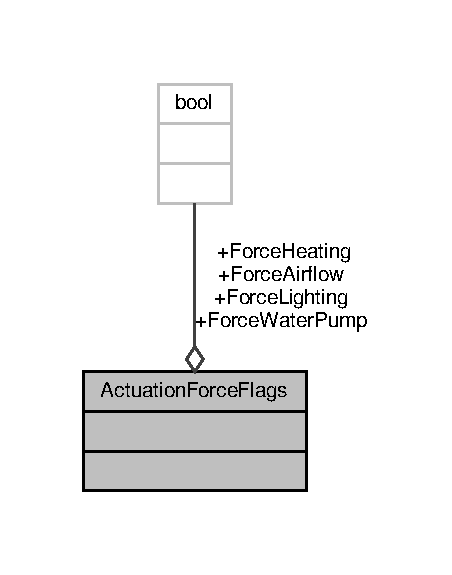
\includegraphics[width=217pt]{structActuationForceFlags__coll__graph}
\end{center}
\end{figure}
\subsection*{Public Attributes}
\begin{DoxyCompactItemize}
\item 
bool \hyperlink{structActuationForceFlags_acfa5f3a1459c151992a2d783b79ea734}{Force\+Heating}
\item 
bool \hyperlink{structActuationForceFlags_a575df93310a4363147c99437d7b8061c}{Force\+Lighting}
\item 
bool \hyperlink{structActuationForceFlags_a6df34a4a82cc2b7297f8a1cbe2e073da}{Force\+Airflow}
\item 
bool \hyperlink{structActuationForceFlags_ab969137846bc6b38bbe3c204e8a4975e}{Force\+Water\+Pump}
\end{DoxyCompactItemize}


\subsection{Detailed Description}
Environment Data Struct Definition

This struct conatins actuaytor 

\subsection{Member Data Documentation}
\mbox{\Hypertarget{structActuationForceFlags_a6df34a4a82cc2b7297f8a1cbe2e073da}\label{structActuationForceFlags_a6df34a4a82cc2b7297f8a1cbe2e073da}} 
\index{Actuation\+Force\+Flags@{Actuation\+Force\+Flags}!Force\+Airflow@{Force\+Airflow}}
\index{Force\+Airflow@{Force\+Airflow}!Actuation\+Force\+Flags@{Actuation\+Force\+Flags}}
\subsubsection{\texorpdfstring{Force\+Airflow}{ForceAirflow}}
{\footnotesize\ttfamily bool Actuation\+Force\+Flags\+::\+Force\+Airflow}

\mbox{\Hypertarget{structActuationForceFlags_acfa5f3a1459c151992a2d783b79ea734}\label{structActuationForceFlags_acfa5f3a1459c151992a2d783b79ea734}} 
\index{Actuation\+Force\+Flags@{Actuation\+Force\+Flags}!Force\+Heating@{Force\+Heating}}
\index{Force\+Heating@{Force\+Heating}!Actuation\+Force\+Flags@{Actuation\+Force\+Flags}}
\subsubsection{\texorpdfstring{Force\+Heating}{ForceHeating}}
{\footnotesize\ttfamily bool Actuation\+Force\+Flags\+::\+Force\+Heating}

Force Heating on actuation handler \mbox{\Hypertarget{structActuationForceFlags_a575df93310a4363147c99437d7b8061c}\label{structActuationForceFlags_a575df93310a4363147c99437d7b8061c}} 
\index{Actuation\+Force\+Flags@{Actuation\+Force\+Flags}!Force\+Lighting@{Force\+Lighting}}
\index{Force\+Lighting@{Force\+Lighting}!Actuation\+Force\+Flags@{Actuation\+Force\+Flags}}
\subsubsection{\texorpdfstring{Force\+Lighting}{ForceLighting}}
{\footnotesize\ttfamily bool Actuation\+Force\+Flags\+::\+Force\+Lighting}

\mbox{\Hypertarget{structActuationForceFlags_ab969137846bc6b38bbe3c204e8a4975e}\label{structActuationForceFlags_ab969137846bc6b38bbe3c204e8a4975e}} 
\index{Actuation\+Force\+Flags@{Actuation\+Force\+Flags}!Force\+Water\+Pump@{Force\+Water\+Pump}}
\index{Force\+Water\+Pump@{Force\+Water\+Pump}!Actuation\+Force\+Flags@{Actuation\+Force\+Flags}}
\subsubsection{\texorpdfstring{Force\+Water\+Pump}{ForceWaterPump}}
{\footnotesize\ttfamily bool Actuation\+Force\+Flags\+::\+Force\+Water\+Pump}



The documentation for this struct was generated from the following file\+:\begin{DoxyCompactItemize}
\item 
src/utils/\hyperlink{typeDefinitions_8h}{type\+Definitions.\+h}\end{DoxyCompactItemize}

\hypertarget{classCamera}{}\section{Camera Class Reference}
\label{classCamera}\index{Camera@{Camera}}


{\ttfamily \#include $<$Camera.\+h$>$}



Inheritance diagram for Camera\+:\nopagebreak
\begin{figure}[H]
\begin{center}
\leavevmode
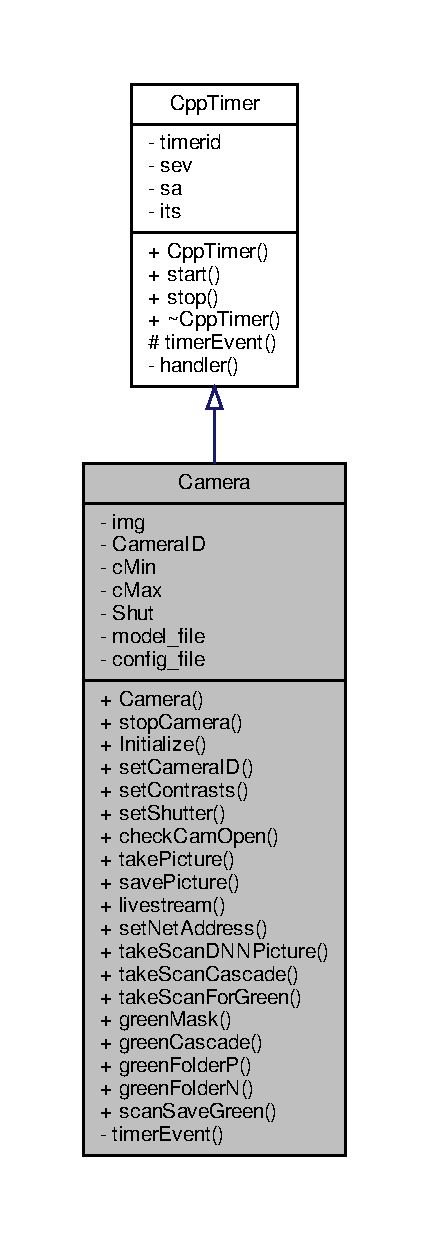
\includegraphics[height=550pt]{classCamera__inherit__graph}
\end{center}
\end{figure}


Collaboration diagram for Camera\+:\nopagebreak
\begin{figure}[H]
\begin{center}
\leavevmode
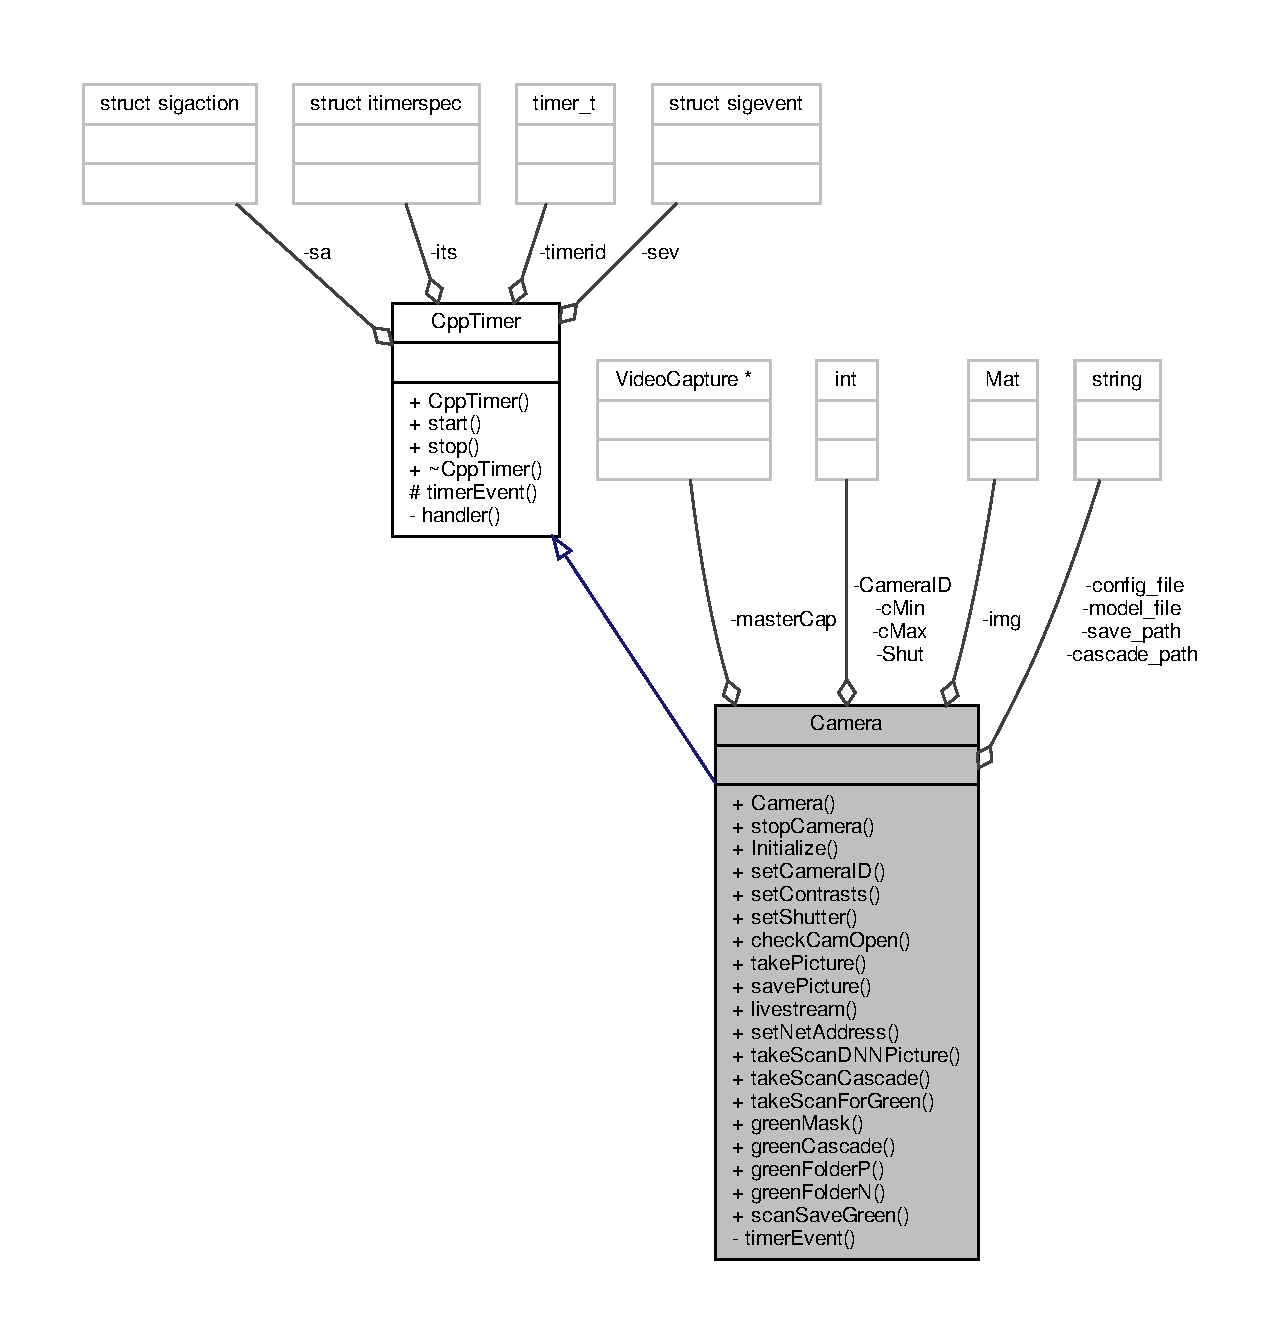
\includegraphics[width=350pt]{classCamera__coll__graph}
\end{center}
\end{figure}
\subsection*{Public Member Functions}
\begin{DoxyCompactItemize}
\item 
\hyperlink{classCamera_a01f94c3543f56ede7af49dc778f19331}{Camera} ()
\item 
void \hyperlink{classCamera_aac0e2e17954d17a0c15019ca74149f15}{stop\+Camera} ()
\item 
void \hyperlink{classCamera_afd88c2780203f02c9fe236a7239e414c}{Initialize} ()
\item 
void \hyperlink{classCamera_af699a1dad54f8631e862b6f7703e48d3}{set\+Camera\+ID} (int ID)
\item 
void \hyperlink{classCamera_aef0a4ebb556d5a2a0f13e5d120c05259}{set\+Contrasts} (int low, int high)
\item 
void \hyperlink{classCamera_a9409482c4422823f73d45b3d5e29304b}{set\+Shutter} (int Shutter)
\item 
int \hyperlink{classCamera_a230bee20d42ae409aba0700d8205bbe0}{check\+Cam\+Open} (cv\+::\+Video\+Capture cap)
\item 
cv\+::\+Mat \hyperlink{classCamera_a07670e99337fb322375a412222c06ada}{take\+Picture} ()
\item 
void \hyperlink{classCamera_ad0c5cc34e0b16ab7925d2c432ece20de}{save\+Picture} (std\+::string filename)
\item 
void \hyperlink{classCamera_af0d3c970e947813e71f316b9e499b456}{livestream} ()
\item 
void \hyperlink{classCamera_a3595618ceff1b74e79633b4132ada11f}{set\+Net\+Address} (std\+::string, std\+::string)
\item 
void \hyperlink{classCamera_a59f08842d3de300419c74b12bee44d47}{take\+Scan\+D\+N\+N\+Picture} ()
\item 
void \hyperlink{classCamera_a09931f84cc8e66e4e4c1181cb1cb4af6}{take\+Scan\+Cascade} ()
\item 
void \hyperlink{classCamera_ab4f4c3f77479c8594dfa7fd7e6348306}{take\+Scan\+For\+Green} ()
\item 
cv\+::\+Mat \hyperlink{classCamera_adf305e574ca94bce9435c217fef1501b}{green\+Mask} (cv\+::\+Mat)
\begin{DoxyCompactList}\small\item\em Takes an image and returns the same image filtered to show green only. \end{DoxyCompactList}\item 
void \hyperlink{classCamera_a5dd9bbe1eac3485d2fb835e21f0d9a9d}{green\+Cascade} (cv\+::\+Mat)
\begin{DoxyCompactList}\small\item\em function to run cascade on a green masked image \end{DoxyCompactList}\item 
void \hyperlink{classCamera_ac8f74b6c456d6fc7e9e83e746f8fc6c5}{green\+FolderP} ()
\item 
void \hyperlink{classCamera_ac212835924bf4cee1b8c477a6b79f4d2}{green\+FolderN} (int)
\item 
void \hyperlink{classCamera_a06cf0ed4a2b79d95637ddeb3301d3856}{scan\+Save\+Green} (std\+::string)
\item 
virtual void \hyperlink{classCppTimer_a64989025caa3c030c6c397ca76a2d20b}{start} (long nanosecs, \hyperlink{CppTimer_8h_a110d07ab6a96d7815149d3d95435790a}{cpp\+Timer\+Type\+\_\+t} type=\hyperlink{CppTimer_8h_a110d07ab6a96d7815149d3d95435790aae4379d044711537d9ce3b3b58c575c58}{P\+E\+R\+I\+O\+D\+IC})
\item 
virtual void \hyperlink{classCppTimer_a4bb95ddee98a536d0818b8f6096bf7e7}{stop} ()
\end{DoxyCompactItemize}
\subsection*{Private Member Functions}
\begin{DoxyCompactItemize}
\item 
void \hyperlink{classCamera_afcf6ca7256cd36f2f4a5ba088d67090a}{timer\+Event} ()
\end{DoxyCompactItemize}
\subsection*{Private Attributes}
\begin{DoxyCompactItemize}
\item 
cv\+::\+Mat \hyperlink{classCamera_a9a184f1522b055612f5ede1cc2443457}{img}
\item 
int \hyperlink{classCamera_a96c19741cb6ba7a897ca90746e8b8918}{Camera\+ID}
\begin{DoxyCompactList}\small\item\em for storing images \end{DoxyCompactList}\item 
int \hyperlink{classCamera_ab6f982f42917eb9ef75606e97fc82911}{c\+Min}
\begin{DoxyCompactList}\small\item\em for setting camera ID, default 0 \end{DoxyCompactList}\item 
int \hyperlink{classCamera_ad784af65b7f7e1b6ebb9b33df774d7db}{c\+Max}
\begin{DoxyCompactList}\small\item\em Minimum contrast for image normalization. \end{DoxyCompactList}\item 
int \hyperlink{classCamera_ad3d6176cdcccecd116f2e7867b642ad1}{Shut} = 0
\begin{DoxyCompactList}\small\item\em Maximmum contrast for image normalization. \end{DoxyCompactList}\item 
std\+::string \hyperlink{classCamera_a22a0754fc359b253e203ce59026021a0}{model\+\_\+file} = \char`\"{}Resources/frozen\+\_\+inference\+\_\+graph.\+pb\char`\"{}
\begin{DoxyCompactList}\small\item\em Shutter speed in ms; 30 is reasonable. \end{DoxyCompactList}\item 
std\+::string \hyperlink{classCamera_affbb5356cbe1e069d4e107ccda0d1b2b}{config\+\_\+file} = \char`\"{}Resources/ssd\+\_\+mobilenet\+\_\+v2\+\_\+coco\+\_\+2018\+\_\+03\+\_\+29.\+pbtxt\char`\"{}
\end{DoxyCompactItemize}


\subsection{Detailed Description}
This class is responsible for taking an image in specified intervals and saving it Inherits from \hyperlink{classCppTimer}{Cpp\+Timer} 

\subsection{Constructor \& Destructor Documentation}
\mbox{\Hypertarget{classCamera_a01f94c3543f56ede7af49dc778f19331}\label{classCamera_a01f94c3543f56ede7af49dc778f19331}} 
\index{Camera@{Camera}!Camera@{Camera}}
\index{Camera@{Camera}!Camera@{Camera}}
\subsubsection{\texorpdfstring{Camera()}{Camera()}}
{\footnotesize\ttfamily Camera\+::\+Camera (\begin{DoxyParamCaption}{ }\end{DoxyParamCaption})\hspace{0.3cm}{\ttfamily [inline]}}



\subsection{Member Function Documentation}
\mbox{\Hypertarget{classCamera_a230bee20d42ae409aba0700d8205bbe0}\label{classCamera_a230bee20d42ae409aba0700d8205bbe0}} 
\index{Camera@{Camera}!check\+Cam\+Open@{check\+Cam\+Open}}
\index{check\+Cam\+Open@{check\+Cam\+Open}!Camera@{Camera}}
\subsubsection{\texorpdfstring{check\+Cam\+Open()}{checkCamOpen()}}
{\footnotesize\ttfamily int Camera\+::check\+Cam\+Open (\begin{DoxyParamCaption}\item[{cv\+::\+Video\+Capture}]{cap }\end{DoxyParamCaption})}

Debug function to chek whether camera is opened successfully. Used within other functions that take pictures/stream.


\begin{DoxyParams}{Parameters}
{\em cap} & Video\+Capture object -\/ essentially which camera is being communicated with\\
\hline
\end{DoxyParams}
\begin{DoxyReturn}{Returns}
int 1 and error message if camera has failed to open, a line of text it successfully opened. 
\end{DoxyReturn}
\mbox{\Hypertarget{classCamera_a5dd9bbe1eac3485d2fb835e21f0d9a9d}\label{classCamera_a5dd9bbe1eac3485d2fb835e21f0d9a9d}} 
\index{Camera@{Camera}!green\+Cascade@{green\+Cascade}}
\index{green\+Cascade@{green\+Cascade}!Camera@{Camera}}
\subsubsection{\texorpdfstring{green\+Cascade()}{greenCascade()}}
{\footnotesize\ttfamily void Camera\+::green\+Cascade (\begin{DoxyParamCaption}\item[{cv\+::\+Mat}]{image }\end{DoxyParamCaption})}



function to run cascade on a green masked image 

\begin{DoxyReturn}{Returns}
a saved image with detections 
\end{DoxyReturn}
\mbox{\Hypertarget{classCamera_ac212835924bf4cee1b8c477a6b79f4d2}\label{classCamera_ac212835924bf4cee1b8c477a6b79f4d2}} 
\index{Camera@{Camera}!green\+FolderN@{green\+FolderN}}
\index{green\+FolderN@{green\+FolderN}!Camera@{Camera}}
\subsubsection{\texorpdfstring{green\+Folder\+N()}{greenFolderN()}}
{\footnotesize\ttfamily void Camera\+::green\+FolderN (\begin{DoxyParamCaption}\item[{int}]{Number }\end{DoxyParamCaption})}

\mbox{\Hypertarget{classCamera_ac8f74b6c456d6fc7e9e83e746f8fc6c5}\label{classCamera_ac8f74b6c456d6fc7e9e83e746f8fc6c5}} 
\index{Camera@{Camera}!green\+FolderP@{green\+FolderP}}
\index{green\+FolderP@{green\+FolderP}!Camera@{Camera}}
\subsubsection{\texorpdfstring{green\+Folder\+P()}{greenFolderP()}}
{\footnotesize\ttfamily void Camera\+::green\+FolderP (\begin{DoxyParamCaption}{ }\end{DoxyParamCaption})}

\mbox{\Hypertarget{classCamera_adf305e574ca94bce9435c217fef1501b}\label{classCamera_adf305e574ca94bce9435c217fef1501b}} 
\index{Camera@{Camera}!green\+Mask@{green\+Mask}}
\index{green\+Mask@{green\+Mask}!Camera@{Camera}}
\subsubsection{\texorpdfstring{green\+Mask()}{greenMask()}}
{\footnotesize\ttfamily cv\+::\+Mat Camera\+::green\+Mask (\begin{DoxyParamCaption}\item[{cv\+::\+Mat}]{image }\end{DoxyParamCaption})}



Takes an image and returns the same image filtered to show green only. 


\begin{DoxyParams}{Parameters}
{\em image} & A cv\+::\+Mat image to be givena green mask \\
\hline
\end{DoxyParams}
\begin{DoxyReturn}{Returns}
cv\+::\+Mat , same as image in but with green mask 
\end{DoxyReturn}
\mbox{\Hypertarget{classCamera_afd88c2780203f02c9fe236a7239e414c}\label{classCamera_afd88c2780203f02c9fe236a7239e414c}} 
\index{Camera@{Camera}!Initialize@{Initialize}}
\index{Initialize@{Initialize}!Camera@{Camera}}
\subsubsection{\texorpdfstring{Initialize()}{Initialize()}}
{\footnotesize\ttfamily void Camera\+::\+Initialize (\begin{DoxyParamCaption}{ }\end{DoxyParamCaption})}


\begin{DoxyParams}{Parameters}
{\em } & \\
\hline
\end{DoxyParams}
\mbox{\Hypertarget{classCamera_af0d3c970e947813e71f316b9e499b456}\label{classCamera_af0d3c970e947813e71f316b9e499b456}} 
\index{Camera@{Camera}!livestream@{livestream}}
\index{livestream@{livestream}!Camera@{Camera}}
\subsubsection{\texorpdfstring{livestream()}{livestream()}}
{\footnotesize\ttfamily void Camera\+::livestream (\begin{DoxyParamCaption}{ }\end{DoxyParamCaption})}

Function to livestream video to an Open\+CV window -\/ requires a G\+UI

\begin{DoxyReturn}{Returns}
an open cv window livestreaming from camera 
\end{DoxyReturn}
\mbox{\Hypertarget{classCamera_ad0c5cc34e0b16ab7925d2c432ece20de}\label{classCamera_ad0c5cc34e0b16ab7925d2c432ece20de}} 
\index{Camera@{Camera}!save\+Picture@{save\+Picture}}
\index{save\+Picture@{save\+Picture}!Camera@{Camera}}
\subsubsection{\texorpdfstring{save\+Picture()}{savePicture()}}
{\footnotesize\ttfamily void Camera\+::save\+Picture (\begin{DoxyParamCaption}\item[{std\+::string}]{filename }\end{DoxyParamCaption})}

Function to take a picture and save it.


\begin{DoxyParams}{Parameters}
{\em filename} & String to save file as.\\
\hline
\end{DoxyParams}
\begin{DoxyReturn}{Returns}
a saved image file as filename.\+jpg 
\end{DoxyReturn}
\mbox{\Hypertarget{classCamera_a06cf0ed4a2b79d95637ddeb3301d3856}\label{classCamera_a06cf0ed4a2b79d95637ddeb3301d3856}} 
\index{Camera@{Camera}!scan\+Save\+Green@{scan\+Save\+Green}}
\index{scan\+Save\+Green@{scan\+Save\+Green}!Camera@{Camera}}
\subsubsection{\texorpdfstring{scan\+Save\+Green()}{scanSaveGreen()}}
{\footnotesize\ttfamily void Camera\+::scan\+Save\+Green (\begin{DoxyParamCaption}\item[{std\+::string}]{filename }\end{DoxyParamCaption})}

\mbox{\Hypertarget{classCamera_af699a1dad54f8631e862b6f7703e48d3}\label{classCamera_af699a1dad54f8631e862b6f7703e48d3}} 
\index{Camera@{Camera}!set\+Camera\+ID@{set\+Camera\+ID}}
\index{set\+Camera\+ID@{set\+Camera\+ID}!Camera@{Camera}}
\subsubsection{\texorpdfstring{set\+Camera\+I\+D()}{setCameraID()}}
{\footnotesize\ttfamily void Camera\+::set\+Camera\+ID (\begin{DoxyParamCaption}\item[{int}]{ID }\end{DoxyParamCaption})}

Set the \hyperlink{classCamera}{Camera} ID object


\begin{DoxyParams}{Parameters}
{\em ID} & \\
\hline
\end{DoxyParams}
\begin{DoxyReturn}{Returns}
updated \hyperlink{classCamera_a96c19741cb6ba7a897ca90746e8b8918}{Camera\+::\+Camera\+ID} 
\end{DoxyReturn}
\mbox{\Hypertarget{classCamera_aef0a4ebb556d5a2a0f13e5d120c05259}\label{classCamera_aef0a4ebb556d5a2a0f13e5d120c05259}} 
\index{Camera@{Camera}!set\+Contrasts@{set\+Contrasts}}
\index{set\+Contrasts@{set\+Contrasts}!Camera@{Camera}}
\subsubsection{\texorpdfstring{set\+Contrasts()}{setContrasts()}}
{\footnotesize\ttfamily void Camera\+::set\+Contrasts (\begin{DoxyParamCaption}\item[{int}]{low,  }\item[{int}]{high }\end{DoxyParamCaption})}

Set the upper and lower contrast in order to work in variable brightnesses


\begin{DoxyParams}{Parameters}
{\em low} & Lower contrast level. 0 is normally ok.\\
\hline
{\em high} & higher contrast level. 400 is usually ok but in dark settings may need to reach 600-\/800.\\
\hline
\end{DoxyParams}
\begin{DoxyReturn}{Returns}
Updated \hyperlink{classCamera_ab6f982f42917eb9ef75606e97fc82911}{Camera\+::c\+Min} and \hyperlink{classCamera_ad784af65b7f7e1b6ebb9b33df774d7db}{Camera\+::c\+Max} 
\end{DoxyReturn}
\mbox{\Hypertarget{classCamera_a3595618ceff1b74e79633b4132ada11f}\label{classCamera_a3595618ceff1b74e79633b4132ada11f}} 
\index{Camera@{Camera}!set\+Net\+Address@{set\+Net\+Address}}
\index{set\+Net\+Address@{set\+Net\+Address}!Camera@{Camera}}
\subsubsection{\texorpdfstring{set\+Net\+Address()}{setNetAddress()}}
{\footnotesize\ttfamily void Camera\+::set\+Net\+Address (\begin{DoxyParamCaption}\item[{std\+::string}]{netpath,  }\item[{std\+::string}]{weightspath }\end{DoxyParamCaption})}

Set neural net pathway


\begin{DoxyParams}{Parameters}
{\em netpath} & Location of neural net\\
\hline
{\em weightspath} & Location of weights\\
\hline
\end{DoxyParams}
\begin{DoxyReturn}{Returns}
updated Camera\+::net\+File and camera\+::weights\+Path 
\end{DoxyReturn}
\mbox{\Hypertarget{classCamera_a9409482c4422823f73d45b3d5e29304b}\label{classCamera_a9409482c4422823f73d45b3d5e29304b}} 
\index{Camera@{Camera}!set\+Shutter@{set\+Shutter}}
\index{set\+Shutter@{set\+Shutter}!Camera@{Camera}}
\subsubsection{\texorpdfstring{set\+Shutter()}{setShutter()}}
{\footnotesize\ttfamily void Camera\+::set\+Shutter (\begin{DoxyParamCaption}\item[{int}]{Shutter }\end{DoxyParamCaption})}

Set the shutter speed. Must be $>$= 1, 30 works for me.


\begin{DoxyParams}{Parameters}
{\em Shutter} & Shutter speed in ms\\
\hline
\end{DoxyParams}
\begin{DoxyReturn}{Returns}
updated \hyperlink{classCamera_ad3d6176cdcccecd116f2e7867b642ad1}{Camera\+::\+Shut} 
\end{DoxyReturn}
\mbox{\Hypertarget{classCppTimer_a64989025caa3c030c6c397ca76a2d20b}\label{classCppTimer_a64989025caa3c030c6c397ca76a2d20b}} 
\index{Camera@{Camera}!start@{start}}
\index{start@{start}!Camera@{Camera}}
\subsubsection{\texorpdfstring{start()}{start()}}
{\footnotesize\ttfamily void Cpp\+Timer\+::start (\begin{DoxyParamCaption}\item[{long}]{nanosecs,  }\item[{\hyperlink{CppTimer_8h_a110d07ab6a96d7815149d3d95435790a}{cpp\+Timer\+Type\+\_\+t}}]{type = {\ttfamily \hyperlink{CppTimer_8h_a110d07ab6a96d7815149d3d95435790aae4379d044711537d9ce3b3b58c575c58}{P\+E\+R\+I\+O\+D\+IC}} }\end{DoxyParamCaption})\hspace{0.3cm}{\ttfamily [virtual]}, {\ttfamily [inherited]}}

Starts the timer. The timer fires first after the specified time in nanoseconds and then at that interval in P\+E\+R\+I\+O\+D\+IC mode. In O\+N\+E\+S\+H\+OT mode the timer fires once after the specified time in nanoseconds. \mbox{\Hypertarget{classCppTimer_a4bb95ddee98a536d0818b8f6096bf7e7}\label{classCppTimer_a4bb95ddee98a536d0818b8f6096bf7e7}} 
\index{Camera@{Camera}!stop@{stop}}
\index{stop@{stop}!Camera@{Camera}}
\subsubsection{\texorpdfstring{stop()}{stop()}}
{\footnotesize\ttfamily void Cpp\+Timer\+::stop (\begin{DoxyParamCaption}{ }\end{DoxyParamCaption})\hspace{0.3cm}{\ttfamily [virtual]}, {\ttfamily [inherited]}}

Stops the timer by disarming it. It can be re-\/started with \hyperlink{classCppTimer_a64989025caa3c030c6c397ca76a2d20b}{start()}. \mbox{\Hypertarget{classCamera_aac0e2e17954d17a0c15019ca74149f15}\label{classCamera_aac0e2e17954d17a0c15019ca74149f15}} 
\index{Camera@{Camera}!stop\+Camera@{stop\+Camera}}
\index{stop\+Camera@{stop\+Camera}!Camera@{Camera}}
\subsubsection{\texorpdfstring{stop\+Camera()}{stopCamera()}}
{\footnotesize\ttfamily void Camera\+::stop\+Camera (\begin{DoxyParamCaption}{ }\end{DoxyParamCaption})\hspace{0.3cm}{\ttfamily [inline]}}

Sets the callback which is called whenever there is new data Stops the data acquistion \mbox{\Hypertarget{classCamera_a07670e99337fb322375a412222c06ada}\label{classCamera_a07670e99337fb322375a412222c06ada}} 
\index{Camera@{Camera}!take\+Picture@{take\+Picture}}
\index{take\+Picture@{take\+Picture}!Camera@{Camera}}
\subsubsection{\texorpdfstring{take\+Picture()}{takePicture()}}
{\footnotesize\ttfamily cv\+::\+Mat Camera\+::take\+Picture (\begin{DoxyParamCaption}{ }\end{DoxyParamCaption})}

Function to take a picture and return the frame as a cv mat

\begin{DoxyReturn}{Returns}
cv\+::\+Mat type image from camera
\end{DoxyReturn}
\begin{DoxyRefDesc}{Todo}
\item[\hyperlink{todo__todo000001}{Todo}]option to change this to return a C\+V\+::\+Mat \end{DoxyRefDesc}
\mbox{\Hypertarget{classCamera_a09931f84cc8e66e4e4c1181cb1cb4af6}\label{classCamera_a09931f84cc8e66e4e4c1181cb1cb4af6}} 
\index{Camera@{Camera}!take\+Scan\+Cascade@{take\+Scan\+Cascade}}
\index{take\+Scan\+Cascade@{take\+Scan\+Cascade}!Camera@{Camera}}
\subsubsection{\texorpdfstring{take\+Scan\+Cascade()}{takeScanCascade()}}
{\footnotesize\ttfamily void Camera\+::take\+Scan\+Cascade (\begin{DoxyParamCaption}{ }\end{DoxyParamCaption})}

Function to take a picture and scan it with a custom H\+A\+AR Cascade. Best option currently.

\begin{DoxyReturn}{Returns}
a saved image with detections
\end{DoxyReturn}
\begin{DoxyRefDesc}{Todo}
\item[\hyperlink{todo__todo000003}{Todo}]keep improving the dataset being used to train the cascade. Try training a cascade on some of the green masked contours images. \end{DoxyRefDesc}
\mbox{\Hypertarget{classCamera_a59f08842d3de300419c74b12bee44d47}\label{classCamera_a59f08842d3de300419c74b12bee44d47}} 
\index{Camera@{Camera}!take\+Scan\+D\+N\+N\+Picture@{take\+Scan\+D\+N\+N\+Picture}}
\index{take\+Scan\+D\+N\+N\+Picture@{take\+Scan\+D\+N\+N\+Picture}!Camera@{Camera}}
\subsubsection{\texorpdfstring{take\+Scan\+D\+N\+N\+Picture()}{takeScanDNNPicture()}}
{\footnotesize\ttfamily void Camera\+::take\+Scan\+D\+N\+N\+Picture (\begin{DoxyParamCaption}{ }\end{DoxyParamCaption})}

Function to take a picture and scan it with a D\+NN built in tensorflow.

\begin{DoxyReturn}{Returns}
a saved image with detections
\end{DoxyReturn}
\begin{DoxyRefDesc}{Todo}
\item[\hyperlink{todo__todo000002}{Todo}]Work out how to get a frozen\+\_\+inference\+\_\+graph.\+pb to work here. For whatever reason, it throws an error at runtime when using custom trained nets. \end{DoxyRefDesc}
\mbox{\Hypertarget{classCamera_ab4f4c3f77479c8594dfa7fd7e6348306}\label{classCamera_ab4f4c3f77479c8594dfa7fd7e6348306}} 
\index{Camera@{Camera}!take\+Scan\+For\+Green@{take\+Scan\+For\+Green}}
\index{take\+Scan\+For\+Green@{take\+Scan\+For\+Green}!Camera@{Camera}}
\subsubsection{\texorpdfstring{take\+Scan\+For\+Green()}{takeScanForGreen()}}
{\footnotesize\ttfamily void Camera\+::take\+Scan\+For\+Green (\begin{DoxyParamCaption}{ }\end{DoxyParamCaption})}

Function to draw a box around anything green. A classifier could be trained on the shapes this picks up. Adds another step, but could be viable.

\begin{DoxyReturn}{Returns}
saved image of green detection
\end{DoxyReturn}
\begin{DoxyRefDesc}{Todo}
\item[\hyperlink{todo__todo000004}{Todo}]create a bunch of images this way. train a cascade on them. run the cascade again. \end{DoxyRefDesc}
\mbox{\Hypertarget{classCamera_afcf6ca7256cd36f2f4a5ba088d67090a}\label{classCamera_afcf6ca7256cd36f2f4a5ba088d67090a}} 
\index{Camera@{Camera}!timer\+Event@{timer\+Event}}
\index{timer\+Event@{timer\+Event}!Camera@{Camera}}
\subsubsection{\texorpdfstring{timer\+Event()}{timerEvent()}}
{\footnotesize\ttfamily void Camera\+::timer\+Event (\begin{DoxyParamCaption}{ }\end{DoxyParamCaption})\hspace{0.3cm}{\ttfamily [inline]}, {\ttfamily [private]}, {\ttfamily [virtual]}}

Abstract function which needs to be implemented by the children. This is called every time the timer fires. 

Implements \hyperlink{classCppTimer_ac2665403595b6aee5f581d0ebfeb886c}{Cpp\+Timer}.



\subsection{Member Data Documentation}
\mbox{\Hypertarget{classCamera_a96c19741cb6ba7a897ca90746e8b8918}\label{classCamera_a96c19741cb6ba7a897ca90746e8b8918}} 
\index{Camera@{Camera}!Camera\+ID@{Camera\+ID}}
\index{Camera\+ID@{Camera\+ID}!Camera@{Camera}}
\subsubsection{\texorpdfstring{Camera\+ID}{CameraID}}
{\footnotesize\ttfamily int Camera\+::\+Camera\+ID\hspace{0.3cm}{\ttfamily [private]}}



for storing images 

\mbox{\Hypertarget{classCamera_ad784af65b7f7e1b6ebb9b33df774d7db}\label{classCamera_ad784af65b7f7e1b6ebb9b33df774d7db}} 
\index{Camera@{Camera}!c\+Max@{c\+Max}}
\index{c\+Max@{c\+Max}!Camera@{Camera}}
\subsubsection{\texorpdfstring{c\+Max}{cMax}}
{\footnotesize\ttfamily int Camera\+::c\+Max\hspace{0.3cm}{\ttfamily [private]}}



Minimum contrast for image normalization. 

\mbox{\Hypertarget{classCamera_ab6f982f42917eb9ef75606e97fc82911}\label{classCamera_ab6f982f42917eb9ef75606e97fc82911}} 
\index{Camera@{Camera}!c\+Min@{c\+Min}}
\index{c\+Min@{c\+Min}!Camera@{Camera}}
\subsubsection{\texorpdfstring{c\+Min}{cMin}}
{\footnotesize\ttfamily int Camera\+::c\+Min\hspace{0.3cm}{\ttfamily [private]}}



for setting camera ID, default 0 

\mbox{\Hypertarget{classCamera_affbb5356cbe1e069d4e107ccda0d1b2b}\label{classCamera_affbb5356cbe1e069d4e107ccda0d1b2b}} 
\index{Camera@{Camera}!config\+\_\+file@{config\+\_\+file}}
\index{config\+\_\+file@{config\+\_\+file}!Camera@{Camera}}
\subsubsection{\texorpdfstring{config\+\_\+file}{config\_file}}
{\footnotesize\ttfamily std\+::string Camera\+::config\+\_\+file = \char`\"{}Resources/ssd\+\_\+mobilenet\+\_\+v2\+\_\+coco\+\_\+2018\+\_\+03\+\_\+29.\+pbtxt\char`\"{}\hspace{0.3cm}{\ttfamily [private]}}

\mbox{\Hypertarget{classCamera_a9a184f1522b055612f5ede1cc2443457}\label{classCamera_a9a184f1522b055612f5ede1cc2443457}} 
\index{Camera@{Camera}!img@{img}}
\index{img@{img}!Camera@{Camera}}
\subsubsection{\texorpdfstring{img}{img}}
{\footnotesize\ttfamily cv\+::\+Mat Camera\+::img\hspace{0.3cm}{\ttfamily [private]}}

\mbox{\Hypertarget{classCamera_a22a0754fc359b253e203ce59026021a0}\label{classCamera_a22a0754fc359b253e203ce59026021a0}} 
\index{Camera@{Camera}!model\+\_\+file@{model\+\_\+file}}
\index{model\+\_\+file@{model\+\_\+file}!Camera@{Camera}}
\subsubsection{\texorpdfstring{model\+\_\+file}{model\_file}}
{\footnotesize\ttfamily std\+::string Camera\+::model\+\_\+file = \char`\"{}Resources/frozen\+\_\+inference\+\_\+graph.\+pb\char`\"{}\hspace{0.3cm}{\ttfamily [private]}}



Shutter speed in ms; 30 is reasonable. 

\mbox{\Hypertarget{classCamera_ad3d6176cdcccecd116f2e7867b642ad1}\label{classCamera_ad3d6176cdcccecd116f2e7867b642ad1}} 
\index{Camera@{Camera}!Shut@{Shut}}
\index{Shut@{Shut}!Camera@{Camera}}
\subsubsection{\texorpdfstring{Shut}{Shut}}
{\footnotesize\ttfamily int Camera\+::\+Shut = 0\hspace{0.3cm}{\ttfamily [private]}}



Maximmum contrast for image normalization. 



The documentation for this class was generated from the following files\+:\begin{DoxyCompactItemize}
\item 
src/controller/peripherials/\hyperlink{Camera_8h}{Camera.\+h}\item 
src/controller/peripherials/\hyperlink{Camera_8cpp}{Camera.\+cpp}\end{DoxyCompactItemize}

\hypertarget{classController}{}\section{Controller Class Reference}
\label{classController}\index{Controller@{Controller}}


\hyperlink{classController}{Controller} class.  




{\ttfamily \#include $<$Controller.\+h$>$}



Collaboration diagram for Controller\+:\nopagebreak
\begin{figure}[H]
\begin{center}
\leavevmode
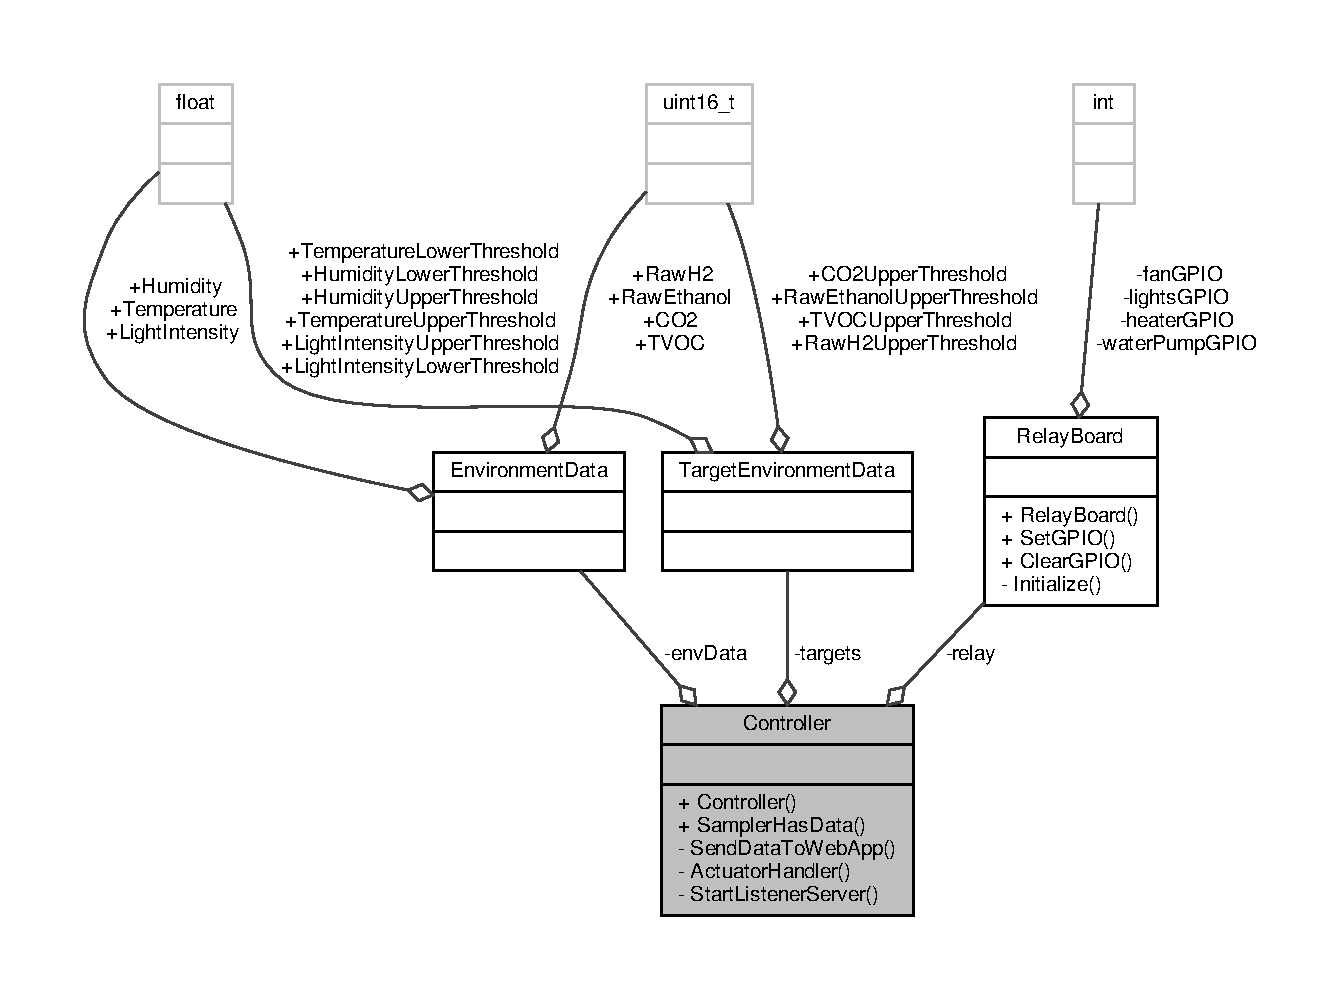
\includegraphics[width=350pt]{classController__coll__graph}
\end{center}
\end{figure}
\subsection*{Public Member Functions}
\begin{DoxyCompactItemize}
\item 
\hyperlink{classController_a95c56822d667e94b031451729ce069a9}{Controller} ()
\item 
void \hyperlink{classController_a4b765eaaf8f72e964118967f86c265e2}{Sampler\+Has\+Data} (\hyperlink{structEnvironmentData}{Environment\+Data} new\+Data)
\item 
int \hyperlink{classController_a0eb08a1d38b2c79e2d140476fd097f24}{Update\+\_\+\+Targets} (uint8\+\_\+t opcode, float vlaue)
\item 
void \hyperlink{classController_a64173dd00be020975d7db533cd280c15}{Start\+Listener\+Server} ()
\item 
void \hyperlink{classController_affbf340fed1aca0172f336bcb2db8c8a}{Message\+Handler} (uint8\+\_\+t opcode, float value)
\end{DoxyCompactItemize}
\subsection*{Public Attributes}
\begin{DoxyCompactItemize}
\item 
\hyperlink{structEnvironmentData}{Environment\+Data} \hyperlink{classController_ac99088334f56588243867ca1c18f9633}{env\+Data}
\item 
\hyperlink{structTargetEnvironmentData}{Target\+Environment\+Data} \hyperlink{classController_a8f2fb8295fd3da6ebc8bdb0f25036322}{targets}
\item 
\hyperlink{structActuationForceFlags}{Actuation\+Force\+Flags} \hyperlink{classController_adb38d16eaea1f98887b3c1fc75ab5bd3}{actuation\+Flags}
\end{DoxyCompactItemize}
\subsection*{Private Types}
\begin{DoxyCompactItemize}
\item 
enum \hyperlink{classController_ae0cc6feb81bc46e0859390fd1551ff43}{T\+A\+R\+G\+E\+T\+\_\+\+O\+P\+\_\+\+C\+O\+D\+ES} \{ \newline
\hyperlink{classController_ae0cc6feb81bc46e0859390fd1551ff43a915722d1485a0a671e6d9740e4f336d7}{L\+I\+G\+H\+T\+\_\+\+I\+N\+T\+E\+N\+S\+I\+T\+Y\+\_\+\+T\+A\+R\+G\+E\+T\+\_\+\+C\+H\+A\+N\+GE} = 1, 
\hyperlink{classController_ae0cc6feb81bc46e0859390fd1551ff43a1c6726567b0f23f4431b2b2693b67ec9}{T\+E\+M\+P\+E\+R\+A\+T\+U\+R\+E\+\_\+\+T\+A\+R\+G\+E\+T\+\_\+\+C\+H\+A\+N\+GE} = 2, 
\hyperlink{classController_ae0cc6feb81bc46e0859390fd1551ff43a9380620e3b95492374b3ac3a3e3bd5e7}{H\+U\+M\+I\+D\+I\+T\+Y\+\_\+\+T\+A\+R\+G\+E\+T\+\_\+\+C\+H\+A\+N\+GE} = 3, 
\hyperlink{classController_ae0cc6feb81bc46e0859390fd1551ff43ab7367a898dd3e0befa174fa4e42f1eeb}{T\+V\+O\+C\+\_\+\+T\+A\+R\+G\+E\+T\+\_\+\+C\+H\+A\+N\+GE} = 4, 
\newline
\hyperlink{classController_ae0cc6feb81bc46e0859390fd1551ff43af162eb21304384728b51aad12ef581c3}{E\+C\+O2\+\_\+\+T\+A\+R\+G\+E\+T\+\_\+\+C\+H\+A\+N\+GE} = 5, 
\hyperlink{classController_ae0cc6feb81bc46e0859390fd1551ff43a93b6d3178783a23734c076d193fcb1fb}{E\+T\+H\+\_\+\+T\+A\+R\+G\+E\+T\+\_\+\+C\+H\+A\+N\+GE} = 6, 
\hyperlink{classController_ae0cc6feb81bc46e0859390fd1551ff43a19170325b57f14dd6d349184ed1379e2}{H2\+\_\+\+T\+A\+R\+G\+E\+T\+\_\+\+C\+H\+A\+N\+GE} = 7
 \}
\end{DoxyCompactItemize}
\subsection*{Private Member Functions}
\begin{DoxyCompactItemize}
\item 
void \hyperlink{classController_a9d59ef3807f630a52c964a899a7235dd}{Send\+Data\+To\+Web\+App} (std\+::string variable\+\_\+type, float value)
\item 
void \hyperlink{classController_acd0145853d19eaf3ef9d15f6203ace69}{Actuator\+Handler} ()
\end{DoxyCompactItemize}
\subsection*{Private Attributes}
\begin{DoxyCompactItemize}
\item 
\hyperlink{classRelayBoard}{Relay\+Board} \hyperlink{classController_aa3f1d7aae706a5440adf520cbd7fb216}{relay}
\end{DoxyCompactItemize}


\subsection{Detailed Description}
\hyperlink{classController}{Controller} class. 

\begin{DoxyAuthor}{Author}
Kamil Rog
\end{DoxyAuthor}
This is class is responsilbe for the \hyperlink{classSHT31D}{S\+H\+T31D} temperature and humidity sensor.\hypertarget{classController_PROTOCOL}{}\subsection{P\+R\+O\+T\+O\+C\+OL}\label{classController_PROTOCOL}
W\+A\+T\+ER P\+U\+MP -\/ A\+N\+A\+L\+OG -\/ G\+P\+IO x H\+E\+A\+T\+ER -\/ A\+N\+A\+L\+OG -\/ G\+P\+IO x 

\subsection{Member Enumeration Documentation}
\mbox{\Hypertarget{classController_ae0cc6feb81bc46e0859390fd1551ff43}\label{classController_ae0cc6feb81bc46e0859390fd1551ff43}} 
\index{Controller@{Controller}!T\+A\+R\+G\+E\+T\+\_\+\+O\+P\+\_\+\+C\+O\+D\+ES@{T\+A\+R\+G\+E\+T\+\_\+\+O\+P\+\_\+\+C\+O\+D\+ES}}
\index{T\+A\+R\+G\+E\+T\+\_\+\+O\+P\+\_\+\+C\+O\+D\+ES@{T\+A\+R\+G\+E\+T\+\_\+\+O\+P\+\_\+\+C\+O\+D\+ES}!Controller@{Controller}}
\subsubsection{\texorpdfstring{T\+A\+R\+G\+E\+T\+\_\+\+O\+P\+\_\+\+C\+O\+D\+ES}{TARGET\_OP\_CODES}}
{\footnotesize\ttfamily enum \hyperlink{classController_ae0cc6feb81bc46e0859390fd1551ff43}{Controller\+::\+T\+A\+R\+G\+E\+T\+\_\+\+O\+P\+\_\+\+C\+O\+D\+ES}\hspace{0.3cm}{\ttfamily [private]}}

\begin{DoxyEnumFields}{Enumerator}
\raisebox{\heightof{T}}[0pt][0pt]{\index{L\+I\+G\+H\+T\+\_\+\+I\+N\+T\+E\+N\+S\+I\+T\+Y\+\_\+\+T\+A\+R\+G\+E\+T\+\_\+\+C\+H\+A\+N\+GE@{L\+I\+G\+H\+T\+\_\+\+I\+N\+T\+E\+N\+S\+I\+T\+Y\+\_\+\+T\+A\+R\+G\+E\+T\+\_\+\+C\+H\+A\+N\+GE}!Controller@{Controller}}\index{Controller@{Controller}!L\+I\+G\+H\+T\+\_\+\+I\+N\+T\+E\+N\+S\+I\+T\+Y\+\_\+\+T\+A\+R\+G\+E\+T\+\_\+\+C\+H\+A\+N\+GE@{L\+I\+G\+H\+T\+\_\+\+I\+N\+T\+E\+N\+S\+I\+T\+Y\+\_\+\+T\+A\+R\+G\+E\+T\+\_\+\+C\+H\+A\+N\+GE}}}\mbox{\Hypertarget{classController_ae0cc6feb81bc46e0859390fd1551ff43a915722d1485a0a671e6d9740e4f336d7}\label{classController_ae0cc6feb81bc46e0859390fd1551ff43a915722d1485a0a671e6d9740e4f336d7}} 
L\+I\+G\+H\+T\+\_\+\+I\+N\+T\+E\+N\+S\+I\+T\+Y\+\_\+\+T\+A\+R\+G\+E\+T\+\_\+\+C\+H\+A\+N\+GE&\\
\hline

\raisebox{\heightof{T}}[0pt][0pt]{\index{T\+E\+M\+P\+E\+R\+A\+T\+U\+R\+E\+\_\+\+T\+A\+R\+G\+E\+T\+\_\+\+C\+H\+A\+N\+GE@{T\+E\+M\+P\+E\+R\+A\+T\+U\+R\+E\+\_\+\+T\+A\+R\+G\+E\+T\+\_\+\+C\+H\+A\+N\+GE}!Controller@{Controller}}\index{Controller@{Controller}!T\+E\+M\+P\+E\+R\+A\+T\+U\+R\+E\+\_\+\+T\+A\+R\+G\+E\+T\+\_\+\+C\+H\+A\+N\+GE@{T\+E\+M\+P\+E\+R\+A\+T\+U\+R\+E\+\_\+\+T\+A\+R\+G\+E\+T\+\_\+\+C\+H\+A\+N\+GE}}}\mbox{\Hypertarget{classController_ae0cc6feb81bc46e0859390fd1551ff43a1c6726567b0f23f4431b2b2693b67ec9}\label{classController_ae0cc6feb81bc46e0859390fd1551ff43a1c6726567b0f23f4431b2b2693b67ec9}} 
T\+E\+M\+P\+E\+R\+A\+T\+U\+R\+E\+\_\+\+T\+A\+R\+G\+E\+T\+\_\+\+C\+H\+A\+N\+GE&\\
\hline

\raisebox{\heightof{T}}[0pt][0pt]{\index{H\+U\+M\+I\+D\+I\+T\+Y\+\_\+\+T\+A\+R\+G\+E\+T\+\_\+\+C\+H\+A\+N\+GE@{H\+U\+M\+I\+D\+I\+T\+Y\+\_\+\+T\+A\+R\+G\+E\+T\+\_\+\+C\+H\+A\+N\+GE}!Controller@{Controller}}\index{Controller@{Controller}!H\+U\+M\+I\+D\+I\+T\+Y\+\_\+\+T\+A\+R\+G\+E\+T\+\_\+\+C\+H\+A\+N\+GE@{H\+U\+M\+I\+D\+I\+T\+Y\+\_\+\+T\+A\+R\+G\+E\+T\+\_\+\+C\+H\+A\+N\+GE}}}\mbox{\Hypertarget{classController_ae0cc6feb81bc46e0859390fd1551ff43a9380620e3b95492374b3ac3a3e3bd5e7}\label{classController_ae0cc6feb81bc46e0859390fd1551ff43a9380620e3b95492374b3ac3a3e3bd5e7}} 
H\+U\+M\+I\+D\+I\+T\+Y\+\_\+\+T\+A\+R\+G\+E\+T\+\_\+\+C\+H\+A\+N\+GE&\\
\hline

\raisebox{\heightof{T}}[0pt][0pt]{\index{T\+V\+O\+C\+\_\+\+T\+A\+R\+G\+E\+T\+\_\+\+C\+H\+A\+N\+GE@{T\+V\+O\+C\+\_\+\+T\+A\+R\+G\+E\+T\+\_\+\+C\+H\+A\+N\+GE}!Controller@{Controller}}\index{Controller@{Controller}!T\+V\+O\+C\+\_\+\+T\+A\+R\+G\+E\+T\+\_\+\+C\+H\+A\+N\+GE@{T\+V\+O\+C\+\_\+\+T\+A\+R\+G\+E\+T\+\_\+\+C\+H\+A\+N\+GE}}}\mbox{\Hypertarget{classController_ae0cc6feb81bc46e0859390fd1551ff43ab7367a898dd3e0befa174fa4e42f1eeb}\label{classController_ae0cc6feb81bc46e0859390fd1551ff43ab7367a898dd3e0befa174fa4e42f1eeb}} 
T\+V\+O\+C\+\_\+\+T\+A\+R\+G\+E\+T\+\_\+\+C\+H\+A\+N\+GE&\\
\hline

\raisebox{\heightof{T}}[0pt][0pt]{\index{E\+C\+O2\+\_\+\+T\+A\+R\+G\+E\+T\+\_\+\+C\+H\+A\+N\+GE@{E\+C\+O2\+\_\+\+T\+A\+R\+G\+E\+T\+\_\+\+C\+H\+A\+N\+GE}!Controller@{Controller}}\index{Controller@{Controller}!E\+C\+O2\+\_\+\+T\+A\+R\+G\+E\+T\+\_\+\+C\+H\+A\+N\+GE@{E\+C\+O2\+\_\+\+T\+A\+R\+G\+E\+T\+\_\+\+C\+H\+A\+N\+GE}}}\mbox{\Hypertarget{classController_ae0cc6feb81bc46e0859390fd1551ff43af162eb21304384728b51aad12ef581c3}\label{classController_ae0cc6feb81bc46e0859390fd1551ff43af162eb21304384728b51aad12ef581c3}} 
E\+C\+O2\+\_\+\+T\+A\+R\+G\+E\+T\+\_\+\+C\+H\+A\+N\+GE&\\
\hline

\raisebox{\heightof{T}}[0pt][0pt]{\index{E\+T\+H\+\_\+\+T\+A\+R\+G\+E\+T\+\_\+\+C\+H\+A\+N\+GE@{E\+T\+H\+\_\+\+T\+A\+R\+G\+E\+T\+\_\+\+C\+H\+A\+N\+GE}!Controller@{Controller}}\index{Controller@{Controller}!E\+T\+H\+\_\+\+T\+A\+R\+G\+E\+T\+\_\+\+C\+H\+A\+N\+GE@{E\+T\+H\+\_\+\+T\+A\+R\+G\+E\+T\+\_\+\+C\+H\+A\+N\+GE}}}\mbox{\Hypertarget{classController_ae0cc6feb81bc46e0859390fd1551ff43a93b6d3178783a23734c076d193fcb1fb}\label{classController_ae0cc6feb81bc46e0859390fd1551ff43a93b6d3178783a23734c076d193fcb1fb}} 
E\+T\+H\+\_\+\+T\+A\+R\+G\+E\+T\+\_\+\+C\+H\+A\+N\+GE&\\
\hline

\raisebox{\heightof{T}}[0pt][0pt]{\index{H2\+\_\+\+T\+A\+R\+G\+E\+T\+\_\+\+C\+H\+A\+N\+GE@{H2\+\_\+\+T\+A\+R\+G\+E\+T\+\_\+\+C\+H\+A\+N\+GE}!Controller@{Controller}}\index{Controller@{Controller}!H2\+\_\+\+T\+A\+R\+G\+E\+T\+\_\+\+C\+H\+A\+N\+GE@{H2\+\_\+\+T\+A\+R\+G\+E\+T\+\_\+\+C\+H\+A\+N\+GE}}}\mbox{\Hypertarget{classController_ae0cc6feb81bc46e0859390fd1551ff43a19170325b57f14dd6d349184ed1379e2}\label{classController_ae0cc6feb81bc46e0859390fd1551ff43a19170325b57f14dd6d349184ed1379e2}} 
H2\+\_\+\+T\+A\+R\+G\+E\+T\+\_\+\+C\+H\+A\+N\+GE&\\
\hline

\end{DoxyEnumFields}


\subsection{Constructor \& Destructor Documentation}
\mbox{\Hypertarget{classController_a95c56822d667e94b031451729ce069a9}\label{classController_a95c56822d667e94b031451729ce069a9}} 
\index{Controller@{Controller}!Controller@{Controller}}
\index{Controller@{Controller}!Controller@{Controller}}
\subsubsection{\texorpdfstring{Controller()}{Controller()}}
{\footnotesize\ttfamily Controller\+::\+Controller (\begin{DoxyParamCaption}{ }\end{DoxyParamCaption})\hspace{0.3cm}{\ttfamily [inline]}}



\subsection{Member Function Documentation}
\mbox{\Hypertarget{classController_acd0145853d19eaf3ef9d15f6203ace69}\label{classController_acd0145853d19eaf3ef9d15f6203ace69}} 
\index{Controller@{Controller}!Actuator\+Handler@{Actuator\+Handler}}
\index{Actuator\+Handler@{Actuator\+Handler}!Controller@{Controller}}
\subsubsection{\texorpdfstring{Actuator\+Handler()}{ActuatorHandler()}}
{\footnotesize\ttfamily void Controller\+::\+Actuator\+Handler (\begin{DoxyParamCaption}{ }\end{DoxyParamCaption})\hspace{0.3cm}{\ttfamily [private]}}

\mbox{\Hypertarget{classController_affbf340fed1aca0172f336bcb2db8c8a}\label{classController_affbf340fed1aca0172f336bcb2db8c8a}} 
\index{Controller@{Controller}!Message\+Handler@{Message\+Handler}}
\index{Message\+Handler@{Message\+Handler}!Controller@{Controller}}
\subsubsection{\texorpdfstring{Message\+Handler()}{MessageHandler()}}
{\footnotesize\ttfamily void Controller\+::\+Message\+Handler (\begin{DoxyParamCaption}\item[{uint8\+\_\+t}]{opcode,  }\item[{float}]{value }\end{DoxyParamCaption})}

\mbox{\Hypertarget{classController_a4b765eaaf8f72e964118967f86c265e2}\label{classController_a4b765eaaf8f72e964118967f86c265e2}} 
\index{Controller@{Controller}!Sampler\+Has\+Data@{Sampler\+Has\+Data}}
\index{Sampler\+Has\+Data@{Sampler\+Has\+Data}!Controller@{Controller}}
\subsubsection{\texorpdfstring{Sampler\+Has\+Data()}{SamplerHasData()}}
{\footnotesize\ttfamily void Controller\+::\+Sampler\+Has\+Data (\begin{DoxyParamCaption}\item[{\hyperlink{structEnvironmentData}{Environment\+Data}}]{new\+Data }\end{DoxyParamCaption})}

\mbox{\Hypertarget{classController_a9d59ef3807f630a52c964a899a7235dd}\label{classController_a9d59ef3807f630a52c964a899a7235dd}} 
\index{Controller@{Controller}!Send\+Data\+To\+Web\+App@{Send\+Data\+To\+Web\+App}}
\index{Send\+Data\+To\+Web\+App@{Send\+Data\+To\+Web\+App}!Controller@{Controller}}
\subsubsection{\texorpdfstring{Send\+Data\+To\+Web\+App()}{SendDataToWebApp()}}
{\footnotesize\ttfamily void Controller\+::\+Send\+Data\+To\+Web\+App (\begin{DoxyParamCaption}\item[{std\+::string}]{variable\+\_\+type,  }\item[{float}]{value }\end{DoxyParamCaption})\hspace{0.3cm}{\ttfamily [private]}}

\mbox{\Hypertarget{classController_a64173dd00be020975d7db533cd280c15}\label{classController_a64173dd00be020975d7db533cd280c15}} 
\index{Controller@{Controller}!Start\+Listener\+Server@{Start\+Listener\+Server}}
\index{Start\+Listener\+Server@{Start\+Listener\+Server}!Controller@{Controller}}
\subsubsection{\texorpdfstring{Start\+Listener\+Server()}{StartListenerServer()}}
{\footnotesize\ttfamily void Controller\+::\+Start\+Listener\+Server (\begin{DoxyParamCaption}{ }\end{DoxyParamCaption})}

\mbox{\Hypertarget{classController_a0eb08a1d38b2c79e2d140476fd097f24}\label{classController_a0eb08a1d38b2c79e2d140476fd097f24}} 
\index{Controller@{Controller}!Update\+\_\+\+Targets@{Update\+\_\+\+Targets}}
\index{Update\+\_\+\+Targets@{Update\+\_\+\+Targets}!Controller@{Controller}}
\subsubsection{\texorpdfstring{Update\+\_\+\+Targets()}{Update\_Targets()}}
{\footnotesize\ttfamily int Controller\+::\+Update\+\_\+\+Targets (\begin{DoxyParamCaption}\item[{uint8\+\_\+t}]{opcode,  }\item[{float}]{vlaue }\end{DoxyParamCaption})}



\subsection{Member Data Documentation}
\mbox{\Hypertarget{classController_adb38d16eaea1f98887b3c1fc75ab5bd3}\label{classController_adb38d16eaea1f98887b3c1fc75ab5bd3}} 
\index{Controller@{Controller}!actuation\+Flags@{actuation\+Flags}}
\index{actuation\+Flags@{actuation\+Flags}!Controller@{Controller}}
\subsubsection{\texorpdfstring{actuation\+Flags}{actuationFlags}}
{\footnotesize\ttfamily \hyperlink{structActuationForceFlags}{Actuation\+Force\+Flags} Controller\+::actuation\+Flags}

Actuatuion force flags ignoring hu Enviroment Conditions \mbox{\Hypertarget{classController_ac99088334f56588243867ca1c18f9633}\label{classController_ac99088334f56588243867ca1c18f9633}} 
\index{Controller@{Controller}!env\+Data@{env\+Data}}
\index{env\+Data@{env\+Data}!Controller@{Controller}}
\subsubsection{\texorpdfstring{env\+Data}{envData}}
{\footnotesize\ttfamily \hyperlink{structEnvironmentData}{Environment\+Data} Controller\+::env\+Data}

Current Enviroment Conditions Read Froms the sensors \mbox{\Hypertarget{classController_aa3f1d7aae706a5440adf520cbd7fb216}\label{classController_aa3f1d7aae706a5440adf520cbd7fb216}} 
\index{Controller@{Controller}!relay@{relay}}
\index{relay@{relay}!Controller@{Controller}}
\subsubsection{\texorpdfstring{relay}{relay}}
{\footnotesize\ttfamily \hyperlink{classRelayBoard}{Relay\+Board} Controller\+::relay\hspace{0.3cm}{\ttfamily [private]}}

\mbox{\Hypertarget{classController_a8f2fb8295fd3da6ebc8bdb0f25036322}\label{classController_a8f2fb8295fd3da6ebc8bdb0f25036322}} 
\index{Controller@{Controller}!targets@{targets}}
\index{targets@{targets}!Controller@{Controller}}
\subsubsection{\texorpdfstring{targets}{targets}}
{\footnotesize\ttfamily \hyperlink{structTargetEnvironmentData}{Target\+Environment\+Data} Controller\+::targets}

Target Enviroment Conditions 

The documentation for this class was generated from the following files\+:\begin{DoxyCompactItemize}
\item 
src/controller/\hyperlink{Controller_8h}{Controller.\+h}\item 
src/controller/\hyperlink{Controller_8cpp}{Controller.\+cpp}\end{DoxyCompactItemize}

\hypertarget{classControllerThread}{}\section{Controller\+Thread Class Reference}
\label{classControllerThread}\index{Controller\+Thread@{Controller\+Thread}}


Server Thread class.  




{\ttfamily \#include $<$Controller\+Thread.\+h$>$}



Inheritance diagram for Controller\+Thread\+:\nopagebreak
\begin{figure}[H]
\begin{center}
\leavevmode
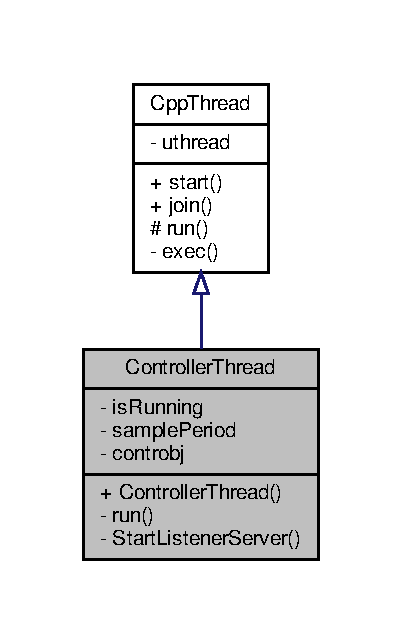
\includegraphics[width=184pt]{classControllerThread__inherit__graph}
\end{center}
\end{figure}


Collaboration diagram for Controller\+Thread\+:\nopagebreak
\begin{figure}[H]
\begin{center}
\leavevmode
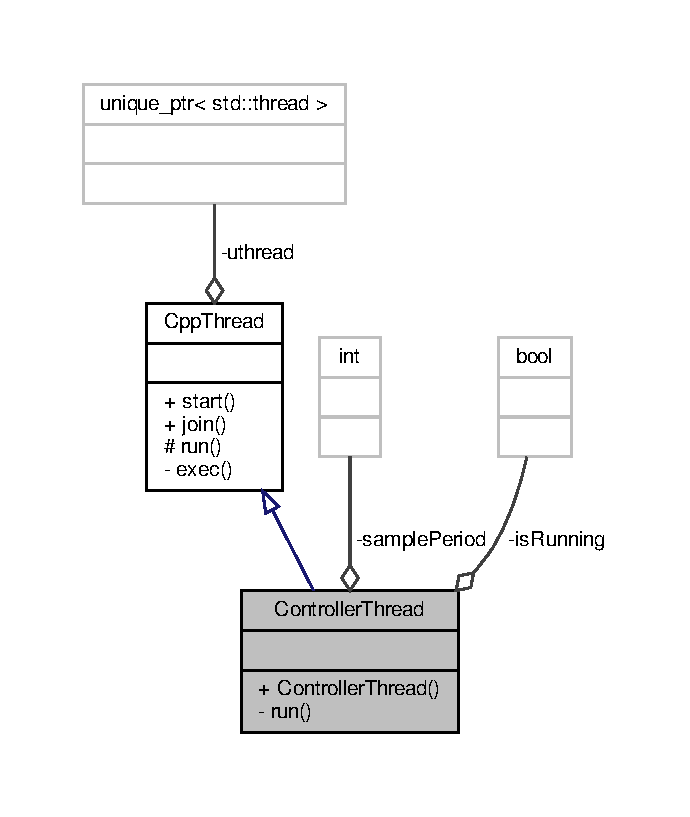
\includegraphics[width=265pt]{classControllerThread__coll__graph}
\end{center}
\end{figure}
\subsection*{Public Member Functions}
\begin{DoxyCompactItemize}
\item 
\hyperlink{classControllerThread_a00cd6502504f5f1e680e6be3f60a987d}{Controller\+Thread} ()
\item 
void \hyperlink{classCppThread_a1be46d1be000f41a763289300623c609}{start} ()
\item 
void \hyperlink{classCppThread_a8ff0fda6b913cc53764caef0e1200f3f}{join} ()
\end{DoxyCompactItemize}
\subsection*{Private Member Functions}
\begin{DoxyCompactItemize}
\item 
void \hyperlink{classControllerThread_ae8206a23ab1a414f2956424def2e759c}{run} ()
\end{DoxyCompactItemize}
\subsection*{Private Attributes}
\begin{DoxyCompactItemize}
\item 
int \hyperlink{classControllerThread_a5dcd0069c7d31295c7e1e598c31fadf7}{sample\+Period}
\end{DoxyCompactItemize}


\subsection{Detailed Description}
Server Thread class. 

\begin{DoxyAuthor}{Author}
Kamil Rog
\end{DoxyAuthor}
This is a simple class that is responsible for data handling for server and files. 

\subsection{Constructor \& Destructor Documentation}
\mbox{\Hypertarget{classControllerThread_a00cd6502504f5f1e680e6be3f60a987d}\label{classControllerThread_a00cd6502504f5f1e680e6be3f60a987d}} 
\index{Controller\+Thread@{Controller\+Thread}!Controller\+Thread@{Controller\+Thread}}
\index{Controller\+Thread@{Controller\+Thread}!Controller\+Thread@{Controller\+Thread}}
\subsubsection{\texorpdfstring{Controller\+Thread()}{ControllerThread()}}
{\footnotesize\ttfamily Controller\+Thread\+::\+Controller\+Thread (\begin{DoxyParamCaption}{ }\end{DoxyParamCaption})\hspace{0.3cm}{\ttfamily [inline]}}

Constructor that sets the sample period(in ms). 

\subsection{Member Function Documentation}
\mbox{\Hypertarget{classCppThread_a8ff0fda6b913cc53764caef0e1200f3f}\label{classCppThread_a8ff0fda6b913cc53764caef0e1200f3f}} 
\index{Controller\+Thread@{Controller\+Thread}!join@{join}}
\index{join@{join}!Controller\+Thread@{Controller\+Thread}}
\subsubsection{\texorpdfstring{join()}{join()}}
{\footnotesize\ttfamily void Cpp\+Thread\+::join (\begin{DoxyParamCaption}{ }\end{DoxyParamCaption})\hspace{0.3cm}{\ttfamily [inline]}, {\ttfamily [inherited]}}

Waits for the thread to terminate. \mbox{\Hypertarget{classControllerThread_ae8206a23ab1a414f2956424def2e759c}\label{classControllerThread_ae8206a23ab1a414f2956424def2e759c}} 
\index{Controller\+Thread@{Controller\+Thread}!run@{run}}
\index{run@{run}!Controller\+Thread@{Controller\+Thread}}
\subsubsection{\texorpdfstring{run()}{run()}}
{\footnotesize\ttfamily void Controller\+Thread\+::run (\begin{DoxyParamCaption}{ }\end{DoxyParamCaption})\hspace{0.3cm}{\ttfamily [private]}, {\ttfamily [virtual]}}

This method does all the work of this thread. Overload this abstract function with a real one doing the actual work of this thread. 

Implements \hyperlink{classCppThread_a792b79e72250710147c452648def4a78}{Cpp\+Thread}.

\mbox{\Hypertarget{classCppThread_a1be46d1be000f41a763289300623c609}\label{classCppThread_a1be46d1be000f41a763289300623c609}} 
\index{Controller\+Thread@{Controller\+Thread}!start@{start}}
\index{start@{start}!Controller\+Thread@{Controller\+Thread}}
\subsubsection{\texorpdfstring{start()}{start()}}
{\footnotesize\ttfamily void Cpp\+Thread\+::start (\begin{DoxyParamCaption}{ }\end{DoxyParamCaption})\hspace{0.3cm}{\ttfamily [inline]}, {\ttfamily [inherited]}}

Starts the thread. 

\subsection{Member Data Documentation}
\mbox{\Hypertarget{classControllerThread_a5dcd0069c7d31295c7e1e598c31fadf7}\label{classControllerThread_a5dcd0069c7d31295c7e1e598c31fadf7}} 
\index{Controller\+Thread@{Controller\+Thread}!sample\+Period@{sample\+Period}}
\index{sample\+Period@{sample\+Period}!Controller\+Thread@{Controller\+Thread}}
\subsubsection{\texorpdfstring{sample\+Period}{samplePeriod}}
{\footnotesize\ttfamily int Controller\+Thread\+::sample\+Period\hspace{0.3cm}{\ttfamily [private]}}



The documentation for this class was generated from the following files\+:\begin{DoxyCompactItemize}
\item 
src/threads/\hyperlink{ControllerThread_8h}{Controller\+Thread.\+h}\item 
src/threads/\hyperlink{ControllerThread_8cpp}{Controller\+Thread.\+cpp}\end{DoxyCompactItemize}

\hypertarget{classCppThread}{}\section{Cpp\+Thread Class Reference}
\label{classCppThread}\index{Cpp\+Thread@{Cpp\+Thread}}


{\ttfamily \#include $<$Cpp\+Thread.\+h$>$}



Inheritance diagram for Cpp\+Thread\+:\nopagebreak
\begin{figure}[H]
\begin{center}
\leavevmode
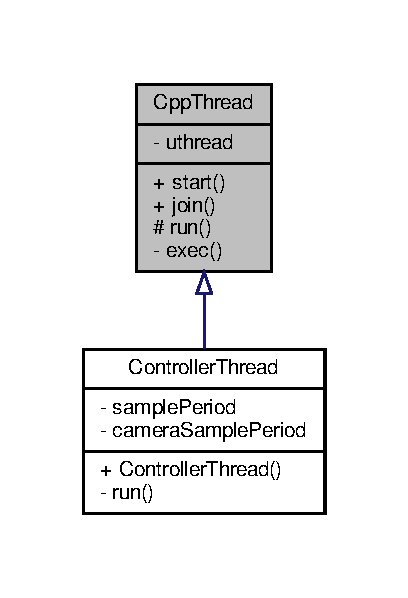
\includegraphics[width=184pt]{classCppThread__inherit__graph}
\end{center}
\end{figure}


Collaboration diagram for Cpp\+Thread\+:\nopagebreak
\begin{figure}[H]
\begin{center}
\leavevmode
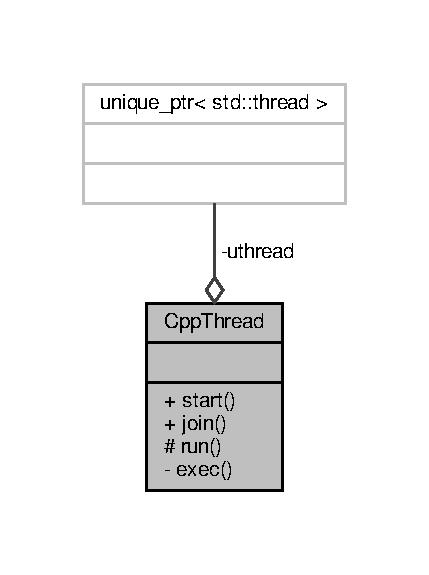
\includegraphics[width=206pt]{classCppThread__coll__graph}
\end{center}
\end{figure}
\subsection*{Public Member Functions}
\begin{DoxyCompactItemize}
\item 
void \hyperlink{classCppThread_a1be46d1be000f41a763289300623c609}{start} ()
\item 
void \hyperlink{classCppThread_a8ff0fda6b913cc53764caef0e1200f3f}{join} ()
\end{DoxyCompactItemize}
\subsection*{Protected Member Functions}
\begin{DoxyCompactItemize}
\item 
virtual void \hyperlink{classCppThread_a792b79e72250710147c452648def4a78}{run} ()=0
\end{DoxyCompactItemize}
\subsection*{Static Private Member Functions}
\begin{DoxyCompactItemize}
\item 
static void \hyperlink{classCppThread_a499b353ef5b5f187ad5eddf638eeb95e}{exec} (\hyperlink{classCppThread}{Cpp\+Thread} $\ast$cpp\+Thread)
\end{DoxyCompactItemize}
\subsection*{Private Attributes}
\begin{DoxyCompactItemize}
\item 
std\+::unique\+\_\+ptr$<$ std\+::thread $>$ \hyperlink{classCppThread_a3136027f60f5054f2a195b7e5fb9f7c9}{uthread} = nullptr
\end{DoxyCompactItemize}


\subsection{Detailed Description}
G\+NU G\+E\+N\+E\+R\+AL P\+U\+B\+L\+IC L\+I\+C\+E\+N\+SE Version 3, 29 June 2007

(C) 2020-\/2021, Bernd Porr \href{mailto:mail@bernporr.me.uk}{\tt mail@bernporr.\+me.\+uk} A thin wrapper around the C++ thread model to avoid a static callback. Instead just inherit this class and overload \hyperlink{classCppThread_a792b79e72250710147c452648def4a78}{run()} which then runs in this thread. This is header-\/only so that it can be performed inline for max performance. 

\subsection{Member Function Documentation}
\mbox{\Hypertarget{classCppThread_a499b353ef5b5f187ad5eddf638eeb95e}\label{classCppThread_a499b353ef5b5f187ad5eddf638eeb95e}} 
\index{Cpp\+Thread@{Cpp\+Thread}!exec@{exec}}
\index{exec@{exec}!Cpp\+Thread@{Cpp\+Thread}}
\subsubsection{\texorpdfstring{exec()}{exec()}}
{\footnotesize\ttfamily static void Cpp\+Thread\+::exec (\begin{DoxyParamCaption}\item[{\hyperlink{classCppThread}{Cpp\+Thread} $\ast$}]{cpp\+Thread }\end{DoxyParamCaption})\hspace{0.3cm}{\ttfamily [inline]}, {\ttfamily [static]}, {\ttfamily [private]}}

\mbox{\Hypertarget{classCppThread_a8ff0fda6b913cc53764caef0e1200f3f}\label{classCppThread_a8ff0fda6b913cc53764caef0e1200f3f}} 
\index{Cpp\+Thread@{Cpp\+Thread}!join@{join}}
\index{join@{join}!Cpp\+Thread@{Cpp\+Thread}}
\subsubsection{\texorpdfstring{join()}{join()}}
{\footnotesize\ttfamily void Cpp\+Thread\+::join (\begin{DoxyParamCaption}{ }\end{DoxyParamCaption})\hspace{0.3cm}{\ttfamily [inline]}}

Waits for the thread to terminate. \mbox{\Hypertarget{classCppThread_a792b79e72250710147c452648def4a78}\label{classCppThread_a792b79e72250710147c452648def4a78}} 
\index{Cpp\+Thread@{Cpp\+Thread}!run@{run}}
\index{run@{run}!Cpp\+Thread@{Cpp\+Thread}}
\subsubsection{\texorpdfstring{run()}{run()}}
{\footnotesize\ttfamily virtual void Cpp\+Thread\+::run (\begin{DoxyParamCaption}{ }\end{DoxyParamCaption})\hspace{0.3cm}{\ttfamily [protected]}, {\ttfamily [pure virtual]}}

This method does all the work of this thread. Overload this abstract function with a real one doing the actual work of this thread. 

Implemented in \hyperlink{classControllerThread_ae8206a23ab1a414f2956424def2e759c}{Controller\+Thread}.

\mbox{\Hypertarget{classCppThread_a1be46d1be000f41a763289300623c609}\label{classCppThread_a1be46d1be000f41a763289300623c609}} 
\index{Cpp\+Thread@{Cpp\+Thread}!start@{start}}
\index{start@{start}!Cpp\+Thread@{Cpp\+Thread}}
\subsubsection{\texorpdfstring{start()}{start()}}
{\footnotesize\ttfamily void Cpp\+Thread\+::start (\begin{DoxyParamCaption}{ }\end{DoxyParamCaption})\hspace{0.3cm}{\ttfamily [inline]}}

Starts the thread. 

\subsection{Member Data Documentation}
\mbox{\Hypertarget{classCppThread_a3136027f60f5054f2a195b7e5fb9f7c9}\label{classCppThread_a3136027f60f5054f2a195b7e5fb9f7c9}} 
\index{Cpp\+Thread@{Cpp\+Thread}!uthread@{uthread}}
\index{uthread@{uthread}!Cpp\+Thread@{Cpp\+Thread}}
\subsubsection{\texorpdfstring{uthread}{uthread}}
{\footnotesize\ttfamily std\+::unique\+\_\+ptr$<$std\+::thread$>$ Cpp\+Thread\+::uthread = nullptr\hspace{0.3cm}{\ttfamily [private]}}



The documentation for this class was generated from the following file\+:\begin{DoxyCompactItemize}
\item 
src/threads/\hyperlink{CppThread_8h}{Cpp\+Thread.\+h}\end{DoxyCompactItemize}

\hypertarget{classCppTimer}{}\section{Cpp\+Timer Class Reference}
\label{classCppTimer}\index{Cpp\+Timer@{Cpp\+Timer}}


{\ttfamily \#include $<$Cpp\+Timer.\+h$>$}



Inheritance diagram for Cpp\+Timer\+:\nopagebreak
\begin{figure}[H]
\begin{center}
\leavevmode
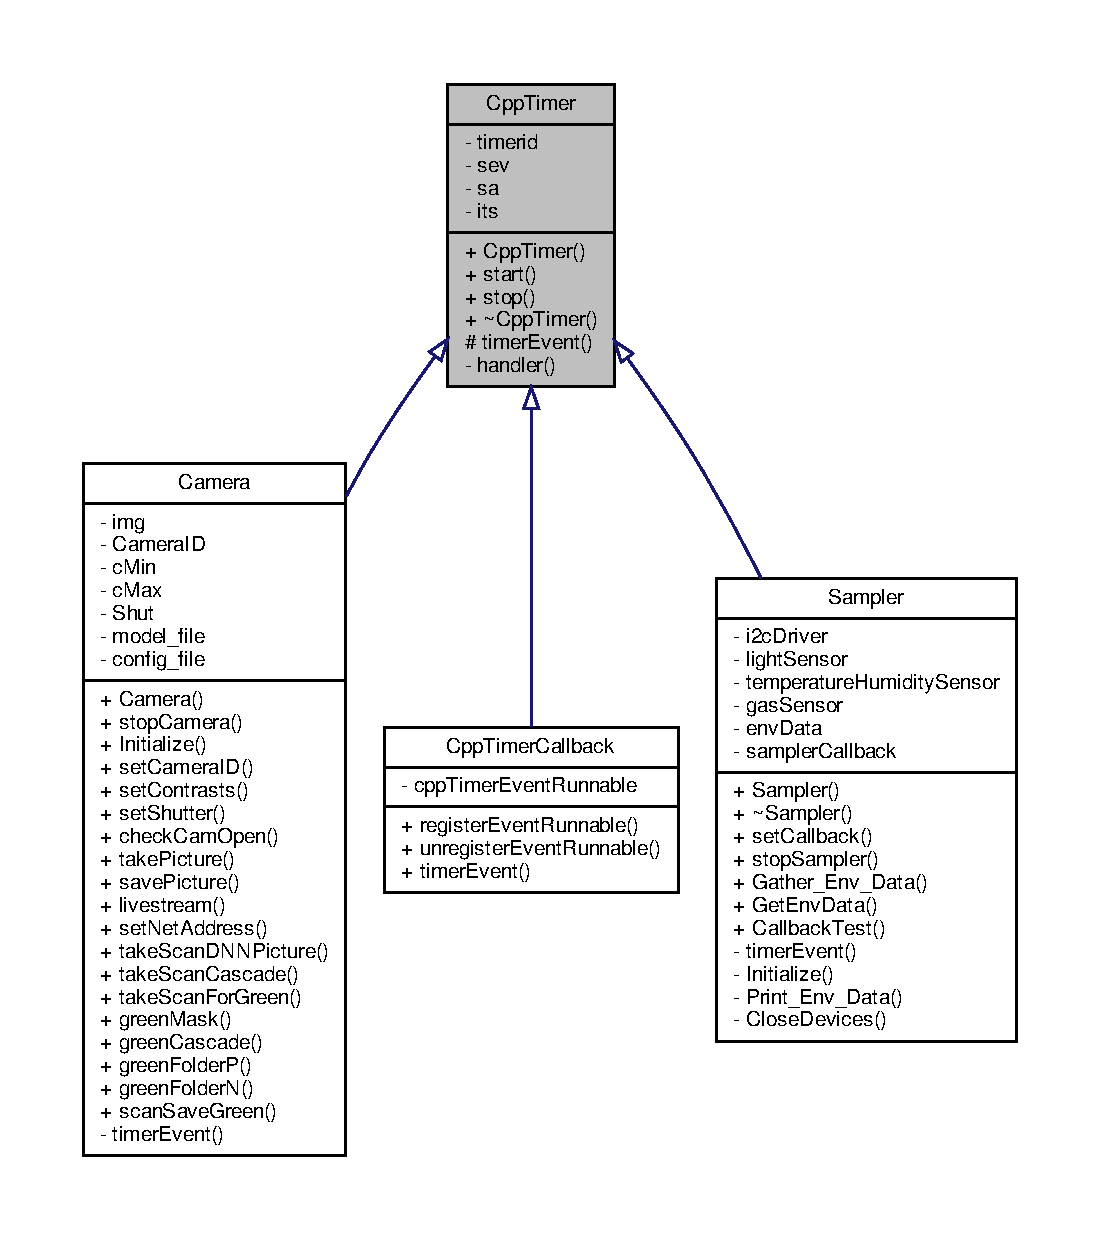
\includegraphics[width=350pt]{classCppTimer__inherit__graph}
\end{center}
\end{figure}


Collaboration diagram for Cpp\+Timer\+:\nopagebreak
\begin{figure}[H]
\begin{center}
\leavevmode
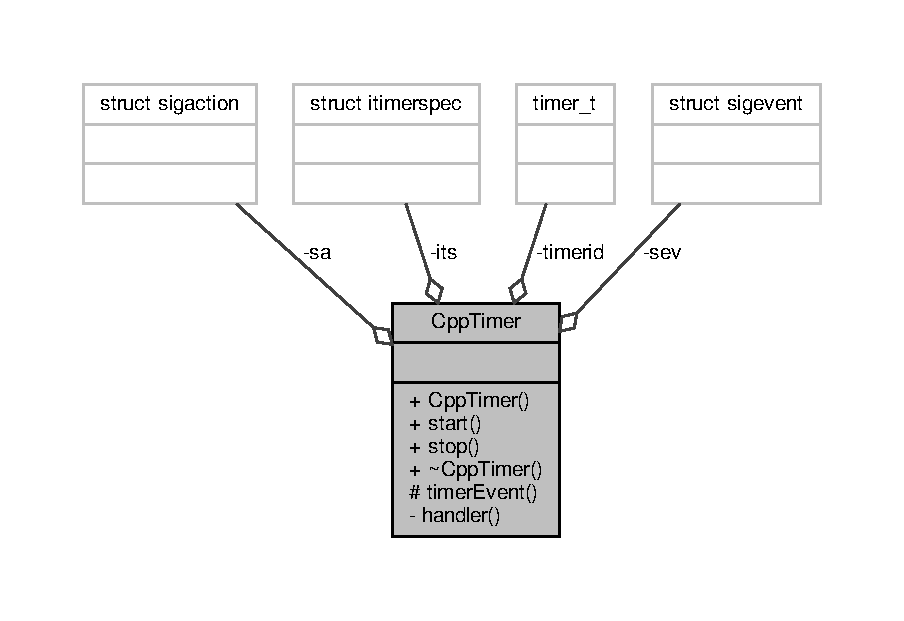
\includegraphics[width=350pt]{classCppTimer__coll__graph}
\end{center}
\end{figure}
\subsection*{Public Member Functions}
\begin{DoxyCompactItemize}
\item 
\hyperlink{classCppTimer_a327a07c051b9b60fcc61e6fd8f40f381}{Cpp\+Timer} ()
\item 
virtual void \hyperlink{classCppTimer_a64989025caa3c030c6c397ca76a2d20b}{start} (long nanosecs, \hyperlink{CppTimer_8h_a110d07ab6a96d7815149d3d95435790a}{cpp\+Timer\+Type\+\_\+t} type=\hyperlink{CppTimer_8h_a110d07ab6a96d7815149d3d95435790aae4379d044711537d9ce3b3b58c575c58}{P\+E\+R\+I\+O\+D\+IC})
\item 
virtual void \hyperlink{classCppTimer_a4bb95ddee98a536d0818b8f6096bf7e7}{stop} ()
\item 
virtual \hyperlink{classCppTimer_a91779a93fce7383a8d832ed481399342}{$\sim$\+Cpp\+Timer} ()
\end{DoxyCompactItemize}
\subsection*{Protected Member Functions}
\begin{DoxyCompactItemize}
\item 
virtual void \hyperlink{classCppTimer_ac2665403595b6aee5f581d0ebfeb886c}{timer\+Event} ()=0
\end{DoxyCompactItemize}
\subsection*{Static Private Member Functions}
\begin{DoxyCompactItemize}
\item 
static void \hyperlink{classCppTimer_a7cf621a640ea9a1e567ee295c7255b5d}{handler} (int sig, siginfo\+\_\+t $\ast$si, void $\ast$uc)
\end{DoxyCompactItemize}
\subsection*{Private Attributes}
\begin{DoxyCompactItemize}
\item 
timer\+\_\+t \hyperlink{classCppTimer_a90ff764263fdde5a0f6e53429c8cf734}{timerid} = 0
\item 
struct sigevent \hyperlink{classCppTimer_a9860d3d723ad55982db50c9cde8d725a}{sev}
\item 
struct sigaction \hyperlink{classCppTimer_a692a200df6d2c43b72ff1db76458f09f}{sa}
\item 
struct itimerspec \hyperlink{classCppTimer_a8774fb5ba9af8f276874c1234741f106}{its}
\end{DoxyCompactItemize}


\subsection{Detailed Description}
Timer class which repeatedly fires. It\textquotesingle{}s wrapper around the P\+O\+S\+IX per-\/process timer. 

\subsection{Constructor \& Destructor Documentation}
\mbox{\Hypertarget{classCppTimer_a327a07c051b9b60fcc61e6fd8f40f381}\label{classCppTimer_a327a07c051b9b60fcc61e6fd8f40f381}} 
\index{Cpp\+Timer@{Cpp\+Timer}!Cpp\+Timer@{Cpp\+Timer}}
\index{Cpp\+Timer@{Cpp\+Timer}!Cpp\+Timer@{Cpp\+Timer}}
\subsubsection{\texorpdfstring{Cpp\+Timer()}{CppTimer()}}
{\footnotesize\ttfamily Cpp\+Timer\+::\+Cpp\+Timer (\begin{DoxyParamCaption}{ }\end{DoxyParamCaption})}

Creates an instance of the timer and connects the signal handler to the timer.

G\+NU G\+E\+N\+E\+R\+AL P\+U\+B\+L\+IC L\+I\+C\+E\+N\+SE Version 3, 29 June 2007

(C) 2020, Bernd Porr \href{mailto:mail@bernporr.me.uk}{\tt mail@bernporr.\+me.\+uk}

This is inspired by the timer\+\_\+create man page. \mbox{\Hypertarget{classCppTimer_a91779a93fce7383a8d832ed481399342}\label{classCppTimer_a91779a93fce7383a8d832ed481399342}} 
\index{Cpp\+Timer@{Cpp\+Timer}!````~Cpp\+Timer@{$\sim$\+Cpp\+Timer}}
\index{````~Cpp\+Timer@{$\sim$\+Cpp\+Timer}!Cpp\+Timer@{Cpp\+Timer}}
\subsubsection{\texorpdfstring{$\sim$\+Cpp\+Timer()}{~CppTimer()}}
{\footnotesize\ttfamily Cpp\+Timer\+::$\sim$\+Cpp\+Timer (\begin{DoxyParamCaption}{ }\end{DoxyParamCaption})\hspace{0.3cm}{\ttfamily [virtual]}}

Destructor disarms the timer, deletes it and disconnect the signal handler. 

\subsection{Member Function Documentation}
\mbox{\Hypertarget{classCppTimer_a7cf621a640ea9a1e567ee295c7255b5d}\label{classCppTimer_a7cf621a640ea9a1e567ee295c7255b5d}} 
\index{Cpp\+Timer@{Cpp\+Timer}!handler@{handler}}
\index{handler@{handler}!Cpp\+Timer@{Cpp\+Timer}}
\subsubsection{\texorpdfstring{handler()}{handler()}}
{\footnotesize\ttfamily static void Cpp\+Timer\+::handler (\begin{DoxyParamCaption}\item[{int}]{sig,  }\item[{siginfo\+\_\+t $\ast$}]{si,  }\item[{void $\ast$}]{uc }\end{DoxyParamCaption})\hspace{0.3cm}{\ttfamily [inline]}, {\ttfamily [static]}, {\ttfamily [private]}}

\mbox{\Hypertarget{classCppTimer_a64989025caa3c030c6c397ca76a2d20b}\label{classCppTimer_a64989025caa3c030c6c397ca76a2d20b}} 
\index{Cpp\+Timer@{Cpp\+Timer}!start@{start}}
\index{start@{start}!Cpp\+Timer@{Cpp\+Timer}}
\subsubsection{\texorpdfstring{start()}{start()}}
{\footnotesize\ttfamily void Cpp\+Timer\+::start (\begin{DoxyParamCaption}\item[{long}]{nanosecs,  }\item[{\hyperlink{CppTimer_8h_a110d07ab6a96d7815149d3d95435790a}{cpp\+Timer\+Type\+\_\+t}}]{type = {\ttfamily \hyperlink{CppTimer_8h_a110d07ab6a96d7815149d3d95435790aae4379d044711537d9ce3b3b58c575c58}{P\+E\+R\+I\+O\+D\+IC}} }\end{DoxyParamCaption})\hspace{0.3cm}{\ttfamily [virtual]}}

Starts the timer. The timer fires first after the specified time in nanoseconds and then at that interval in P\+E\+R\+I\+O\+D\+IC mode. In O\+N\+E\+S\+H\+OT mode the timer fires once after the specified time in nanoseconds. \mbox{\Hypertarget{classCppTimer_a4bb95ddee98a536d0818b8f6096bf7e7}\label{classCppTimer_a4bb95ddee98a536d0818b8f6096bf7e7}} 
\index{Cpp\+Timer@{Cpp\+Timer}!stop@{stop}}
\index{stop@{stop}!Cpp\+Timer@{Cpp\+Timer}}
\subsubsection{\texorpdfstring{stop()}{stop()}}
{\footnotesize\ttfamily void Cpp\+Timer\+::stop (\begin{DoxyParamCaption}{ }\end{DoxyParamCaption})\hspace{0.3cm}{\ttfamily [virtual]}}

Stops the timer by disarming it. It can be re-\/started with \hyperlink{classCppTimer_a64989025caa3c030c6c397ca76a2d20b}{start()}. \mbox{\Hypertarget{classCppTimer_ac2665403595b6aee5f581d0ebfeb886c}\label{classCppTimer_ac2665403595b6aee5f581d0ebfeb886c}} 
\index{Cpp\+Timer@{Cpp\+Timer}!timer\+Event@{timer\+Event}}
\index{timer\+Event@{timer\+Event}!Cpp\+Timer@{Cpp\+Timer}}
\subsubsection{\texorpdfstring{timer\+Event()}{timerEvent()}}
{\footnotesize\ttfamily virtual void Cpp\+Timer\+::timer\+Event (\begin{DoxyParamCaption}{ }\end{DoxyParamCaption})\hspace{0.3cm}{\ttfamily [protected]}, {\ttfamily [pure virtual]}}

Abstract function which needs to be implemented by the children. This is called every time the timer fires. 

Implemented in \hyperlink{classSampler_addf333c6e247ee3a1def41260caa902a}{Sampler}, and \hyperlink{classCppTimerCallback_af6b39f5eb8e98bfc1b301ac3f25276e9}{Cpp\+Timer\+Callback}.



\subsection{Member Data Documentation}
\mbox{\Hypertarget{classCppTimer_a8774fb5ba9af8f276874c1234741f106}\label{classCppTimer_a8774fb5ba9af8f276874c1234741f106}} 
\index{Cpp\+Timer@{Cpp\+Timer}!its@{its}}
\index{its@{its}!Cpp\+Timer@{Cpp\+Timer}}
\subsubsection{\texorpdfstring{its}{its}}
{\footnotesize\ttfamily struct itimerspec Cpp\+Timer\+::its\hspace{0.3cm}{\ttfamily [private]}}

\mbox{\Hypertarget{classCppTimer_a692a200df6d2c43b72ff1db76458f09f}\label{classCppTimer_a692a200df6d2c43b72ff1db76458f09f}} 
\index{Cpp\+Timer@{Cpp\+Timer}!sa@{sa}}
\index{sa@{sa}!Cpp\+Timer@{Cpp\+Timer}}
\subsubsection{\texorpdfstring{sa}{sa}}
{\footnotesize\ttfamily struct sigaction Cpp\+Timer\+::sa\hspace{0.3cm}{\ttfamily [private]}}

\mbox{\Hypertarget{classCppTimer_a9860d3d723ad55982db50c9cde8d725a}\label{classCppTimer_a9860d3d723ad55982db50c9cde8d725a}} 
\index{Cpp\+Timer@{Cpp\+Timer}!sev@{sev}}
\index{sev@{sev}!Cpp\+Timer@{Cpp\+Timer}}
\subsubsection{\texorpdfstring{sev}{sev}}
{\footnotesize\ttfamily struct sigevent Cpp\+Timer\+::sev\hspace{0.3cm}{\ttfamily [private]}}

\mbox{\Hypertarget{classCppTimer_a90ff764263fdde5a0f6e53429c8cf734}\label{classCppTimer_a90ff764263fdde5a0f6e53429c8cf734}} 
\index{Cpp\+Timer@{Cpp\+Timer}!timerid@{timerid}}
\index{timerid@{timerid}!Cpp\+Timer@{Cpp\+Timer}}
\subsubsection{\texorpdfstring{timerid}{timerid}}
{\footnotesize\ttfamily timer\+\_\+t Cpp\+Timer\+::timerid = 0\hspace{0.3cm}{\ttfamily [private]}}



The documentation for this class was generated from the following files\+:\begin{DoxyCompactItemize}
\item 
src/utils/\hyperlink{CppTimer_8h}{Cpp\+Timer.\+h}\item 
src/utils/\hyperlink{CppTimer_8cpp}{Cpp\+Timer.\+cpp}\end{DoxyCompactItemize}

\hypertarget{classCppTimerCallback}{}\section{Cpp\+Timer\+Callback Class Reference}
\label{classCppTimerCallback}\index{Cpp\+Timer\+Callback@{Cpp\+Timer\+Callback}}


{\ttfamily \#include $<$Cpp\+Timer\+Callback.\+h$>$}



Inheritance diagram for Cpp\+Timer\+Callback\+:\nopagebreak
\begin{figure}[H]
\begin{center}
\leavevmode
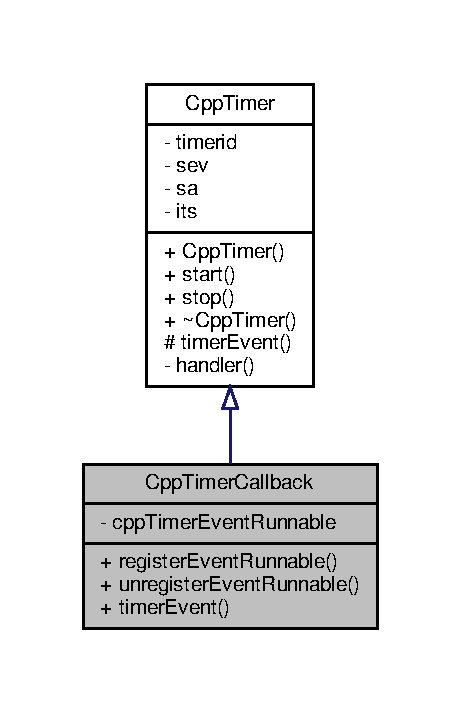
\includegraphics[width=221pt]{classCppTimerCallback__inherit__graph}
\end{center}
\end{figure}


Collaboration diagram for Cpp\+Timer\+Callback\+:\nopagebreak
\begin{figure}[H]
\begin{center}
\leavevmode
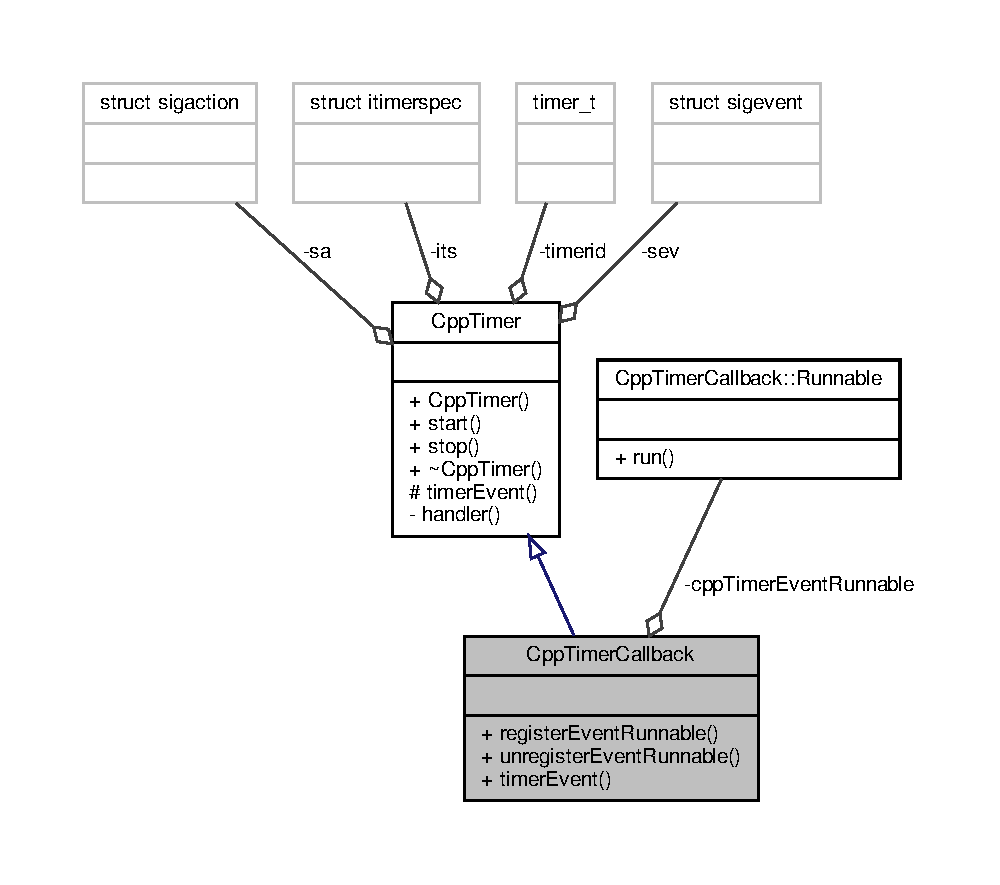
\includegraphics[width=350pt]{classCppTimerCallback__coll__graph}
\end{center}
\end{figure}
\subsection*{Classes}
\begin{DoxyCompactItemize}
\item 
class \hyperlink{classCppTimerCallback_1_1Runnable}{Runnable}
\end{DoxyCompactItemize}
\subsection*{Public Member Functions}
\begin{DoxyCompactItemize}
\item 
void \hyperlink{classCppTimerCallback_ae6e815f1c3b65ea4f10fe0332e13acb9}{register\+Event\+Runnable} (\hyperlink{classCppTimerCallback_1_1Runnable}{Runnable} \&h)
\item 
void \hyperlink{classCppTimerCallback_a29d8d5a426a3d15bca8a42c2c897f50f}{unregister\+Event\+Runnable} ()
\item 
void \hyperlink{classCppTimerCallback_af6b39f5eb8e98bfc1b301ac3f25276e9}{timer\+Event} ()
\item 
virtual void \hyperlink{classCppTimer_a64989025caa3c030c6c397ca76a2d20b}{start} (long nanosecs, \hyperlink{CppTimer_8h_a110d07ab6a96d7815149d3d95435790a}{cpp\+Timer\+Type\+\_\+t} type=\hyperlink{CppTimer_8h_a110d07ab6a96d7815149d3d95435790aae4379d044711537d9ce3b3b58c575c58}{P\+E\+R\+I\+O\+D\+IC})
\item 
virtual void \hyperlink{classCppTimer_a4bb95ddee98a536d0818b8f6096bf7e7}{stop} ()
\end{DoxyCompactItemize}
\subsection*{Private Attributes}
\begin{DoxyCompactItemize}
\item 
\hyperlink{classCppTimerCallback_1_1Runnable}{Runnable} $\ast$ \hyperlink{classCppTimerCallback_a578cc701cee7be10f3afab2859eac74f}{cpp\+Timer\+Event\+Runnable} = N\+U\+LL
\end{DoxyCompactItemize}


\subsection{Member Function Documentation}
\mbox{\Hypertarget{classCppTimerCallback_ae6e815f1c3b65ea4f10fe0332e13acb9}\label{classCppTimerCallback_ae6e815f1c3b65ea4f10fe0332e13acb9}} 
\index{Cpp\+Timer\+Callback@{Cpp\+Timer\+Callback}!register\+Event\+Runnable@{register\+Event\+Runnable}}
\index{register\+Event\+Runnable@{register\+Event\+Runnable}!Cpp\+Timer\+Callback@{Cpp\+Timer\+Callback}}
\subsubsection{\texorpdfstring{register\+Event\+Runnable()}{registerEventRunnable()}}
{\footnotesize\ttfamily void Cpp\+Timer\+Callback\+::register\+Event\+Runnable (\begin{DoxyParamCaption}\item[{\hyperlink{classCppTimerCallback_1_1Runnable}{Runnable} \&}]{h }\end{DoxyParamCaption})\hspace{0.3cm}{\ttfamily [inline]}}

\mbox{\Hypertarget{classCppTimer_a64989025caa3c030c6c397ca76a2d20b}\label{classCppTimer_a64989025caa3c030c6c397ca76a2d20b}} 
\index{Cpp\+Timer\+Callback@{Cpp\+Timer\+Callback}!start@{start}}
\index{start@{start}!Cpp\+Timer\+Callback@{Cpp\+Timer\+Callback}}
\subsubsection{\texorpdfstring{start()}{start()}}
{\footnotesize\ttfamily void Cpp\+Timer\+::start (\begin{DoxyParamCaption}\item[{long}]{nanosecs,  }\item[{\hyperlink{CppTimer_8h_a110d07ab6a96d7815149d3d95435790a}{cpp\+Timer\+Type\+\_\+t}}]{type = {\ttfamily \hyperlink{CppTimer_8h_a110d07ab6a96d7815149d3d95435790aae4379d044711537d9ce3b3b58c575c58}{P\+E\+R\+I\+O\+D\+IC}} }\end{DoxyParamCaption})\hspace{0.3cm}{\ttfamily [virtual]}, {\ttfamily [inherited]}}

Starts the timer. The timer fires first after the specified time in nanoseconds and then at that interval in P\+E\+R\+I\+O\+D\+IC mode. In O\+N\+E\+S\+H\+OT mode the timer fires once after the specified time in nanoseconds. \mbox{\Hypertarget{classCppTimer_a4bb95ddee98a536d0818b8f6096bf7e7}\label{classCppTimer_a4bb95ddee98a536d0818b8f6096bf7e7}} 
\index{Cpp\+Timer\+Callback@{Cpp\+Timer\+Callback}!stop@{stop}}
\index{stop@{stop}!Cpp\+Timer\+Callback@{Cpp\+Timer\+Callback}}
\subsubsection{\texorpdfstring{stop()}{stop()}}
{\footnotesize\ttfamily void Cpp\+Timer\+::stop (\begin{DoxyParamCaption}{ }\end{DoxyParamCaption})\hspace{0.3cm}{\ttfamily [virtual]}, {\ttfamily [inherited]}}

Stops the timer by disarming it. It can be re-\/started with \hyperlink{classCppTimer_a64989025caa3c030c6c397ca76a2d20b}{start()}. \mbox{\Hypertarget{classCppTimerCallback_af6b39f5eb8e98bfc1b301ac3f25276e9}\label{classCppTimerCallback_af6b39f5eb8e98bfc1b301ac3f25276e9}} 
\index{Cpp\+Timer\+Callback@{Cpp\+Timer\+Callback}!timer\+Event@{timer\+Event}}
\index{timer\+Event@{timer\+Event}!Cpp\+Timer\+Callback@{Cpp\+Timer\+Callback}}
\subsubsection{\texorpdfstring{timer\+Event()}{timerEvent()}}
{\footnotesize\ttfamily void Cpp\+Timer\+Callback\+::timer\+Event (\begin{DoxyParamCaption}{ }\end{DoxyParamCaption})\hspace{0.3cm}{\ttfamily [inline]}, {\ttfamily [virtual]}}

Abstract function which needs to be implemented by the children. This is called every time the timer fires. 

Implements \hyperlink{classCppTimer_ac2665403595b6aee5f581d0ebfeb886c}{Cpp\+Timer}.

\mbox{\Hypertarget{classCppTimerCallback_a29d8d5a426a3d15bca8a42c2c897f50f}\label{classCppTimerCallback_a29d8d5a426a3d15bca8a42c2c897f50f}} 
\index{Cpp\+Timer\+Callback@{Cpp\+Timer\+Callback}!unregister\+Event\+Runnable@{unregister\+Event\+Runnable}}
\index{unregister\+Event\+Runnable@{unregister\+Event\+Runnable}!Cpp\+Timer\+Callback@{Cpp\+Timer\+Callback}}
\subsubsection{\texorpdfstring{unregister\+Event\+Runnable()}{unregisterEventRunnable()}}
{\footnotesize\ttfamily void Cpp\+Timer\+Callback\+::unregister\+Event\+Runnable (\begin{DoxyParamCaption}{ }\end{DoxyParamCaption})\hspace{0.3cm}{\ttfamily [inline]}}



\subsection{Member Data Documentation}
\mbox{\Hypertarget{classCppTimerCallback_a578cc701cee7be10f3afab2859eac74f}\label{classCppTimerCallback_a578cc701cee7be10f3afab2859eac74f}} 
\index{Cpp\+Timer\+Callback@{Cpp\+Timer\+Callback}!cpp\+Timer\+Event\+Runnable@{cpp\+Timer\+Event\+Runnable}}
\index{cpp\+Timer\+Event\+Runnable@{cpp\+Timer\+Event\+Runnable}!Cpp\+Timer\+Callback@{Cpp\+Timer\+Callback}}
\subsubsection{\texorpdfstring{cpp\+Timer\+Event\+Runnable}{cppTimerEventRunnable}}
{\footnotesize\ttfamily \hyperlink{classCppTimerCallback_1_1Runnable}{Runnable}$\ast$ Cpp\+Timer\+Callback\+::cpp\+Timer\+Event\+Runnable = N\+U\+LL\hspace{0.3cm}{\ttfamily [private]}}



The documentation for this class was generated from the following file\+:\begin{DoxyCompactItemize}
\item 
src/utils/\hyperlink{CppTimerCallback_8h}{Cpp\+Timer\+Callback.\+h}\end{DoxyCompactItemize}

\hypertarget{structEnvironmentData}{}\section{Environment\+Data Struct Reference}
\label{structEnvironmentData}\index{Environment\+Data@{Environment\+Data}}


{\ttfamily \#include $<$type\+Definitions.\+h$>$}



Collaboration diagram for Environment\+Data\+:\nopagebreak
\begin{figure}[H]
\begin{center}
\leavevmode
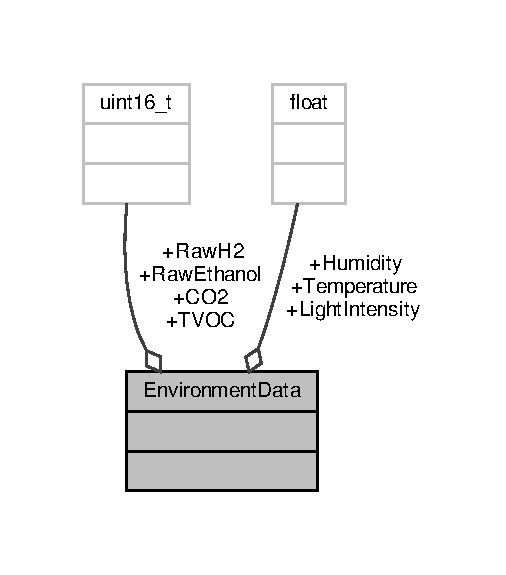
\includegraphics[width=243pt]{structEnvironmentData__coll__graph}
\end{center}
\end{figure}
\subsection*{Public Attributes}
\begin{DoxyCompactItemize}
\item 
float \hyperlink{structEnvironmentData_a2013551c12a584a6680517d750b2116a}{Light\+Intensity}
\begin{DoxyCompactList}\small\item\em Alternativley use triple slash for the comments. \end{DoxyCompactList}\item 
float \hyperlink{structEnvironmentData_a5c8f919b34fe673a71726053d05cb775}{Temperature}
\item 
float \hyperlink{structEnvironmentData_a84e684c2dc15c5fb6bd87a03569cab05}{Humidity}
\item 
uint16\+\_\+t \hyperlink{structEnvironmentData_a5fe69eb57f3debefe5feba3a930ab851}{C\+O2}
\item 
uint16\+\_\+t \hyperlink{structEnvironmentData_aae4ac3338a76432de00582ba5af01a45}{T\+V\+OC}
\item 
uint16\+\_\+t \hyperlink{structEnvironmentData_a3c949734838b0bc862b8f7449b6df41c}{Raw\+Ethanol}
\item 
uint16\+\_\+t \hyperlink{structEnvironmentData_a89c96958697dd39ee2e41289debcd8a5}{Raw\+H2}
\end{DoxyCompactItemize}


\subsection{Detailed Description}
Environment Data Struct Definition

This struct conatins all enviroment data read from sensors as well as target values 

\subsection{Member Data Documentation}
\mbox{\Hypertarget{structEnvironmentData_a5fe69eb57f3debefe5feba3a930ab851}\label{structEnvironmentData_a5fe69eb57f3debefe5feba3a930ab851}} 
\index{Environment\+Data@{Environment\+Data}!C\+O2@{C\+O2}}
\index{C\+O2@{C\+O2}!Environment\+Data@{Environment\+Data}}
\subsubsection{\texorpdfstring{C\+O2}{CO2}}
{\footnotesize\ttfamily uint16\+\_\+t Environment\+Data\+::\+C\+O2}

Carbon Dioxide in air (in ) \mbox{\Hypertarget{structEnvironmentData_a84e684c2dc15c5fb6bd87a03569cab05}\label{structEnvironmentData_a84e684c2dc15c5fb6bd87a03569cab05}} 
\index{Environment\+Data@{Environment\+Data}!Humidity@{Humidity}}
\index{Humidity@{Humidity}!Environment\+Data@{Environment\+Data}}
\subsubsection{\texorpdfstring{Humidity}{Humidity}}
{\footnotesize\ttfamily float Environment\+Data\+::\+Humidity}

Humidity of the environment (in Percent \%) \mbox{\Hypertarget{structEnvironmentData_a2013551c12a584a6680517d750b2116a}\label{structEnvironmentData_a2013551c12a584a6680517d750b2116a}} 
\index{Environment\+Data@{Environment\+Data}!Light\+Intensity@{Light\+Intensity}}
\index{Light\+Intensity@{Light\+Intensity}!Environment\+Data@{Environment\+Data}}
\subsubsection{\texorpdfstring{Light\+Intensity}{LightIntensity}}
{\footnotesize\ttfamily float Environment\+Data\+::\+Light\+Intensity}



Alternativley use triple slash for the comments. 

Light Intensity of the envieronment (in Lux) \mbox{\Hypertarget{structEnvironmentData_a3c949734838b0bc862b8f7449b6df41c}\label{structEnvironmentData_a3c949734838b0bc862b8f7449b6df41c}} 
\index{Environment\+Data@{Environment\+Data}!Raw\+Ethanol@{Raw\+Ethanol}}
\index{Raw\+Ethanol@{Raw\+Ethanol}!Environment\+Data@{Environment\+Data}}
\subsubsection{\texorpdfstring{Raw\+Ethanol}{RawEthanol}}
{\footnotesize\ttfamily uint16\+\_\+t Environment\+Data\+::\+Raw\+Ethanol}

\mbox{\Hypertarget{structEnvironmentData_a89c96958697dd39ee2e41289debcd8a5}\label{structEnvironmentData_a89c96958697dd39ee2e41289debcd8a5}} 
\index{Environment\+Data@{Environment\+Data}!Raw\+H2@{Raw\+H2}}
\index{Raw\+H2@{Raw\+H2}!Environment\+Data@{Environment\+Data}}
\subsubsection{\texorpdfstring{Raw\+H2}{RawH2}}
{\footnotesize\ttfamily uint16\+\_\+t Environment\+Data\+::\+Raw\+H2}

\mbox{\Hypertarget{structEnvironmentData_a5c8f919b34fe673a71726053d05cb775}\label{structEnvironmentData_a5c8f919b34fe673a71726053d05cb775}} 
\index{Environment\+Data@{Environment\+Data}!Temperature@{Temperature}}
\index{Temperature@{Temperature}!Environment\+Data@{Environment\+Data}}
\subsubsection{\texorpdfstring{Temperature}{Temperature}}
{\footnotesize\ttfamily float Environment\+Data\+::\+Temperature}

Temperature of the envirnoment (in Degrees Celsius) \mbox{\Hypertarget{structEnvironmentData_aae4ac3338a76432de00582ba5af01a45}\label{structEnvironmentData_aae4ac3338a76432de00582ba5af01a45}} 
\index{Environment\+Data@{Environment\+Data}!T\+V\+OC@{T\+V\+OC}}
\index{T\+V\+OC@{T\+V\+OC}!Environment\+Data@{Environment\+Data}}
\subsubsection{\texorpdfstring{T\+V\+OC}{TVOC}}
{\footnotesize\ttfamily uint16\+\_\+t Environment\+Data\+::\+T\+V\+OC}

Total Volatile Organic Compounds in air (in ) 

The documentation for this struct was generated from the following file\+:\begin{DoxyCompactItemize}
\item 
src/utils/\hyperlink{typeDefinitions_8h}{type\+Definitions.\+h}\end{DoxyCompactItemize}

\hypertarget{classEventDispatcher}{}\section{Event\+Dispatcher Class Reference}
\label{classEventDispatcher}\index{Event\+Dispatcher@{Event\+Dispatcher}}


Collaboration diagram for Event\+Dispatcher\+:\nopagebreak
\begin{figure}[H]
\begin{center}
\leavevmode
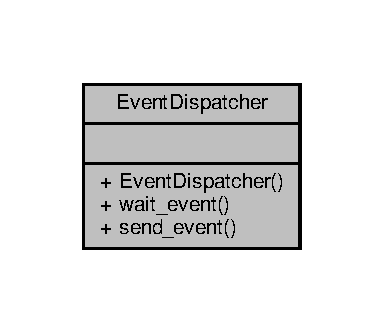
\includegraphics[width=184pt]{classEventDispatcher__coll__graph}
\end{center}
\end{figure}
\subsection*{Public Member Functions}
\begin{DoxyCompactItemize}
\item 
\hyperlink{classEventDispatcher_aec174a9e25796e5727e59f5452817cda}{Event\+Dispatcher} ()
\item 
void \hyperlink{classEventDispatcher_af52dcf785f0c33b88c5b96bb91c6610c}{wait\+\_\+event} (Data\+Sink $\ast$sink)
\item 
void \hyperlink{classEventDispatcher_a17ee873402eb3abbb1e3cd5fa1fadafc}{send\+\_\+event} (const string \&message)
\end{DoxyCompactItemize}


\subsection{Constructor \& Destructor Documentation}
\mbox{\Hypertarget{classEventDispatcher_aec174a9e25796e5727e59f5452817cda}\label{classEventDispatcher_aec174a9e25796e5727e59f5452817cda}} 
\index{Event\+Dispatcher@{Event\+Dispatcher}!Event\+Dispatcher@{Event\+Dispatcher}}
\index{Event\+Dispatcher@{Event\+Dispatcher}!Event\+Dispatcher@{Event\+Dispatcher}}
\subsubsection{\texorpdfstring{Event\+Dispatcher()}{EventDispatcher()}}
{\footnotesize\ttfamily Event\+Dispatcher\+::\+Event\+Dispatcher (\begin{DoxyParamCaption}{ }\end{DoxyParamCaption})\hspace{0.3cm}{\ttfamily [inline]}}



\subsection{Member Function Documentation}
\mbox{\Hypertarget{classEventDispatcher_a17ee873402eb3abbb1e3cd5fa1fadafc}\label{classEventDispatcher_a17ee873402eb3abbb1e3cd5fa1fadafc}} 
\index{Event\+Dispatcher@{Event\+Dispatcher}!send\+\_\+event@{send\+\_\+event}}
\index{send\+\_\+event@{send\+\_\+event}!Event\+Dispatcher@{Event\+Dispatcher}}
\subsubsection{\texorpdfstring{send\+\_\+event()}{send\_event()}}
{\footnotesize\ttfamily void Event\+Dispatcher\+::send\+\_\+event (\begin{DoxyParamCaption}\item[{const string \&}]{message }\end{DoxyParamCaption})\hspace{0.3cm}{\ttfamily [inline]}}

\mbox{\Hypertarget{classEventDispatcher_af52dcf785f0c33b88c5b96bb91c6610c}\label{classEventDispatcher_af52dcf785f0c33b88c5b96bb91c6610c}} 
\index{Event\+Dispatcher@{Event\+Dispatcher}!wait\+\_\+event@{wait\+\_\+event}}
\index{wait\+\_\+event@{wait\+\_\+event}!Event\+Dispatcher@{Event\+Dispatcher}}
\subsubsection{\texorpdfstring{wait\+\_\+event()}{wait\_event()}}
{\footnotesize\ttfamily void Event\+Dispatcher\+::wait\+\_\+event (\begin{DoxyParamCaption}\item[{Data\+Sink $\ast$}]{sink }\end{DoxyParamCaption})\hspace{0.3cm}{\ttfamily [inline]}}



The documentation for this class was generated from the following file\+:\begin{DoxyCompactItemize}
\item 
src/threads/\hyperlink{ControllerThread_8cpp}{Controller\+Thread.\+cpp}\end{DoxyCompactItemize}

\hypertarget{classI2CDriver}{}\section{I2\+C\+Driver Class Reference}
\label{classI2CDriver}\index{I2\+C\+Driver@{I2\+C\+Driver}}


I2C Driver class.  




{\ttfamily \#include $<$I2\+C\+Driver.\+h$>$}



Collaboration diagram for I2\+C\+Driver\+:\nopagebreak
\begin{figure}[H]
\begin{center}
\leavevmode
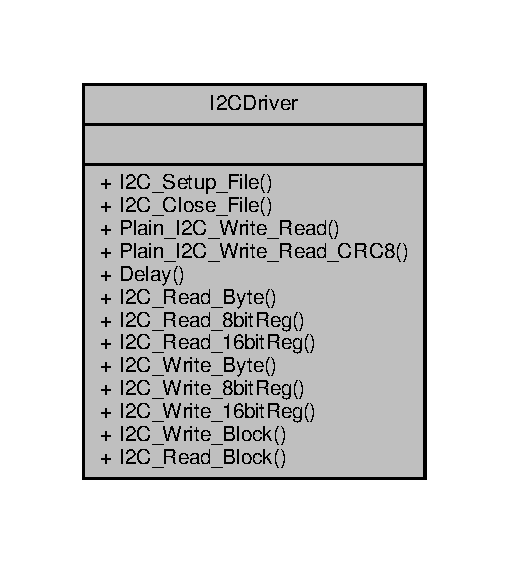
\includegraphics[width=244pt]{classI2CDriver__coll__graph}
\end{center}
\end{figure}
\subsection*{Public Member Functions}
\begin{DoxyCompactItemize}
\item 
int \hyperlink{classI2CDriver_ae25c889f0a2540eee34d53e0228fe914}{I2\+C\+\_\+\+Setup\+\_\+\+File} (int addres)
\item 
int \hyperlink{classI2CDriver_a6480a0e3e5022ac90944f319ca5a5f4e}{I2\+C\+\_\+\+Close\+\_\+\+File} (int fd)
\item 
\hyperlink{I2CDriver_8h_a52c38e7692a76e897b00daa867b29d3f}{I2\+C\+\_\+\+Return} \hyperlink{classI2CDriver_a1e025ccfccece30b7d42acd1bf7e8e41}{Plain\+\_\+\+I2\+C\+\_\+\+Write\+\_\+\+Read} (int fd, uint16\+\_\+t command, uint8\+\_\+t $\ast$buffer, uint8\+\_\+t read\+Length, uint16\+\_\+t delay=10)
\item 
\hyperlink{I2CDriver_8h_a52c38e7692a76e897b00daa867b29d3f}{I2\+C\+\_\+\+Return} \hyperlink{classI2CDriver_a732c5b799a0aecde0d908ee981872572}{Plain\+\_\+\+I2\+C\+\_\+\+Write\+\_\+\+Read\+\_\+\+C\+R\+C8} (int fd, uint16\+\_\+t command, uint16\+\_\+t $\ast$buffer, uint8\+\_\+t readlen, uint16\+\_\+t delay=10)
\item 
void \hyperlink{classI2CDriver_a01453a7adeb358f269faabb33953eee0}{Delay} (unsigned int time\+Ms)
\item 
int \hyperlink{classI2CDriver_acd90c5e9215accc2baf66757054e2906}{I2\+C\+\_\+\+Read\+\_\+\+Byte} (int fd)
\item 
int \hyperlink{classI2CDriver_aab652313af52fe19360bc928baf80fae}{I2\+C\+\_\+\+Read\+\_\+8bit\+Reg} (int fd, int command)
\item 
int \hyperlink{classI2CDriver_a8639cbc95b98be425f6b30dd591384c6}{I2\+C\+\_\+\+Read\+\_\+16bit\+Reg} (int fd, int command)
\item 
int \hyperlink{classI2CDriver_a7b5eb92afa9ed0b5af264836d0944520}{I2\+C\+\_\+\+Write\+\_\+\+Byte} (int fd, int data)
\item 
int \hyperlink{classI2CDriver_a6ff7dfdd4aca26c83c6047f45cce1a9e}{I2\+C\+\_\+\+Write\+\_\+8bit\+Reg} (int fd, int command, int data)
\item 
int \hyperlink{classI2CDriver_a445d2ef0ba5f742fb8264c202dae4a8d}{I2\+C\+\_\+\+Write\+\_\+16bit\+Reg} (int fd, int command, int data)
\item 
int \hyperlink{classI2CDriver_a389bf23234176e0fd0421e078e1fa00d}{I2\+C\+\_\+\+Write\+\_\+\+Block} (int fd, int command, uint8\+\_\+t length, uint8\+\_\+t $\ast$buff)
\item 
int \hyperlink{classI2CDriver_a3877a689d16c30835569c7fa5f064359}{I2\+C\+\_\+\+Read\+\_\+\+Block} (int fd, int command, uint8\+\_\+t $\ast$buff)
\end{DoxyCompactItemize}


\subsection{Detailed Description}
I2C Driver class. 

\begin{DoxyAuthor}{Author}
Kamil Rog
\end{DoxyAuthor}
This is class is responsilbe for handling I2C communication. 

\subsection{Member Function Documentation}
\mbox{\Hypertarget{classI2CDriver_a01453a7adeb358f269faabb33953eee0}\label{classI2CDriver_a01453a7adeb358f269faabb33953eee0}} 
\index{I2\+C\+Driver@{I2\+C\+Driver}!Delay@{Delay}}
\index{Delay@{Delay}!I2\+C\+Driver@{I2\+C\+Driver}}
\subsubsection{\texorpdfstring{Delay()}{Delay()}}
{\footnotesize\ttfamily void I2\+C\+Driver\+::\+Delay (\begin{DoxyParamCaption}\item[{unsigned int}]{time\+Ms }\end{DoxyParamCaption})}

Suspends the execution of the calling thread until at least the time specified has elapsed.


\begin{DoxyParams}{Parameters}
{\em time\+Ms} & Time to wait in miliseconds.\\
\hline
\end{DoxyParams}
\begin{DoxyReturn}{Returns}
none 
\end{DoxyReturn}
\mbox{\Hypertarget{classI2CDriver_a6480a0e3e5022ac90944f319ca5a5f4e}\label{classI2CDriver_a6480a0e3e5022ac90944f319ca5a5f4e}} 
\index{I2\+C\+Driver@{I2\+C\+Driver}!I2\+C\+\_\+\+Close\+\_\+\+File@{I2\+C\+\_\+\+Close\+\_\+\+File}}
\index{I2\+C\+\_\+\+Close\+\_\+\+File@{I2\+C\+\_\+\+Close\+\_\+\+File}!I2\+C\+Driver@{I2\+C\+Driver}}
\subsubsection{\texorpdfstring{I2\+C\+\_\+\+Close\+\_\+\+File()}{I2C\_Close\_File()}}
{\footnotesize\ttfamily int I2\+C\+Driver\+::\+I2\+C\+\_\+\+Close\+\_\+\+File (\begin{DoxyParamCaption}\item[{int}]{fd }\end{DoxyParamCaption})}

Close file descriptor


\begin{DoxyParams}{Parameters}
{\em fd} & File descriptor of the device.\\
\hline
\end{DoxyParams}
\begin{DoxyReturn}{Returns}
result of file descriptor close operation. 
\end{DoxyReturn}
\mbox{\Hypertarget{classI2CDriver_a8639cbc95b98be425f6b30dd591384c6}\label{classI2CDriver_a8639cbc95b98be425f6b30dd591384c6}} 
\index{I2\+C\+Driver@{I2\+C\+Driver}!I2\+C\+\_\+\+Read\+\_\+16bit\+Reg@{I2\+C\+\_\+\+Read\+\_\+16bit\+Reg}}
\index{I2\+C\+\_\+\+Read\+\_\+16bit\+Reg@{I2\+C\+\_\+\+Read\+\_\+16bit\+Reg}!I2\+C\+Driver@{I2\+C\+Driver}}
\subsubsection{\texorpdfstring{I2\+C\+\_\+\+Read\+\_\+16bit\+Reg()}{I2C\_Read\_16bitReg()}}
{\footnotesize\ttfamily int I2\+C\+Driver\+::\+I2\+C\+\_\+\+Read\+\_\+16bit\+Reg (\begin{DoxyParamCaption}\item[{int}]{fd,  }\item[{int}]{command }\end{DoxyParamCaption})}

Use S\+M\+B\+US to Write a byte word and read 2 bytes.


\begin{DoxyParams}{Parameters}
{\em fd} & File descriptor of the device. \\
\hline
{\em command} & Command / Register to address.\\
\hline
\end{DoxyParams}
\begin{DoxyReturn}{Returns}
A 16-\/bit unsigned word received from the device else negative errno 
\end{DoxyReturn}
\mbox{\Hypertarget{classI2CDriver_aab652313af52fe19360bc928baf80fae}\label{classI2CDriver_aab652313af52fe19360bc928baf80fae}} 
\index{I2\+C\+Driver@{I2\+C\+Driver}!I2\+C\+\_\+\+Read\+\_\+8bit\+Reg@{I2\+C\+\_\+\+Read\+\_\+8bit\+Reg}}
\index{I2\+C\+\_\+\+Read\+\_\+8bit\+Reg@{I2\+C\+\_\+\+Read\+\_\+8bit\+Reg}!I2\+C\+Driver@{I2\+C\+Driver}}
\subsubsection{\texorpdfstring{I2\+C\+\_\+\+Read\+\_\+8bit\+Reg()}{I2C\_Read\_8bitReg()}}
{\footnotesize\ttfamily int I2\+C\+Driver\+::\+I2\+C\+\_\+\+Read\+\_\+8bit\+Reg (\begin{DoxyParamCaption}\item[{int}]{fd,  }\item[{int}]{command }\end{DoxyParamCaption})}

Use S\+M\+B\+US to Write a byte word and read one byte from.


\begin{DoxyParams}{Parameters}
{\em fd} & File descriptor of the device. \\
\hline
{\em command} & Command / Register to address.\\
\hline
\end{DoxyParams}
\begin{DoxyReturn}{Returns}
A data byte received from the device elese negative errno. 
\end{DoxyReturn}
\mbox{\Hypertarget{classI2CDriver_a3877a689d16c30835569c7fa5f064359}\label{classI2CDriver_a3877a689d16c30835569c7fa5f064359}} 
\index{I2\+C\+Driver@{I2\+C\+Driver}!I2\+C\+\_\+\+Read\+\_\+\+Block@{I2\+C\+\_\+\+Read\+\_\+\+Block}}
\index{I2\+C\+\_\+\+Read\+\_\+\+Block@{I2\+C\+\_\+\+Read\+\_\+\+Block}!I2\+C\+Driver@{I2\+C\+Driver}}
\subsubsection{\texorpdfstring{I2\+C\+\_\+\+Read\+\_\+\+Block()}{I2C\_Read\_Block()}}
{\footnotesize\ttfamily int I2\+C\+Driver\+::\+I2\+C\+\_\+\+Read\+\_\+\+Block (\begin{DoxyParamCaption}\item[{int}]{fd,  }\item[{int}]{command,  }\item[{uint8\+\_\+t $\ast$}]{buffer }\end{DoxyParamCaption})}

Use S\+M\+B\+US to Read n-\/bytes using a command / addressing specific register.


\begin{DoxyParams}{Parameters}
{\em fd} & File descriptor of the device. \\
\hline
{\em command} & Command / Register to address. \\
\hline
{\em buffer} & Buffer to read the data to.\\
\hline
\end{DoxyParams}
\begin{DoxyReturn}{Returns}
The number of read bytes 
\end{DoxyReturn}
\mbox{\Hypertarget{classI2CDriver_acd90c5e9215accc2baf66757054e2906}\label{classI2CDriver_acd90c5e9215accc2baf66757054e2906}} 
\index{I2\+C\+Driver@{I2\+C\+Driver}!I2\+C\+\_\+\+Read\+\_\+\+Byte@{I2\+C\+\_\+\+Read\+\_\+\+Byte}}
\index{I2\+C\+\_\+\+Read\+\_\+\+Byte@{I2\+C\+\_\+\+Read\+\_\+\+Byte}!I2\+C\+Driver@{I2\+C\+Driver}}
\subsubsection{\texorpdfstring{I2\+C\+\_\+\+Read\+\_\+\+Byte()}{I2C\_Read\_Byte()}}
{\footnotesize\ttfamily int I2\+C\+Driver\+::\+I2\+C\+\_\+\+Read\+\_\+\+Byte (\begin{DoxyParamCaption}\item[{int}]{fd }\end{DoxyParamCaption})}

Use S\+M\+B\+US to read one byte.


\begin{DoxyParams}{Parameters}
{\em fd} & File descriptor of the device.\\
\hline
\end{DoxyParams}
\begin{DoxyReturn}{Returns}
A data byte received from the device elese negative errno. 
\end{DoxyReturn}
\mbox{\Hypertarget{classI2CDriver_ae25c889f0a2540eee34d53e0228fe914}\label{classI2CDriver_ae25c889f0a2540eee34d53e0228fe914}} 
\index{I2\+C\+Driver@{I2\+C\+Driver}!I2\+C\+\_\+\+Setup\+\_\+\+File@{I2\+C\+\_\+\+Setup\+\_\+\+File}}
\index{I2\+C\+\_\+\+Setup\+\_\+\+File@{I2\+C\+\_\+\+Setup\+\_\+\+File}!I2\+C\+Driver@{I2\+C\+Driver}}
\subsubsection{\texorpdfstring{I2\+C\+\_\+\+Setup\+\_\+\+File()}{I2C\_Setup\_File()}}
{\footnotesize\ttfamily int I2\+C\+Driver\+::\+I2\+C\+\_\+\+Setup\+\_\+\+File (\begin{DoxyParamCaption}\item[{int}]{addr }\end{DoxyParamCaption})}

Open I2C File descriptor for target slave device.


\begin{DoxyParams}{Parameters}
{\em addr} & Address of the slave device.\\
\hline
\end{DoxyParams}
\begin{DoxyReturn}{Returns}
I2C File descriptor for specified address of the slave device. 
\end{DoxyReturn}
\mbox{\Hypertarget{classI2CDriver_a445d2ef0ba5f742fb8264c202dae4a8d}\label{classI2CDriver_a445d2ef0ba5f742fb8264c202dae4a8d}} 
\index{I2\+C\+Driver@{I2\+C\+Driver}!I2\+C\+\_\+\+Write\+\_\+16bit\+Reg@{I2\+C\+\_\+\+Write\+\_\+16bit\+Reg}}
\index{I2\+C\+\_\+\+Write\+\_\+16bit\+Reg@{I2\+C\+\_\+\+Write\+\_\+16bit\+Reg}!I2\+C\+Driver@{I2\+C\+Driver}}
\subsubsection{\texorpdfstring{I2\+C\+\_\+\+Write\+\_\+16bit\+Reg()}{I2C\_Write\_16bitReg()}}
{\footnotesize\ttfamily int I2\+C\+Driver\+::\+I2\+C\+\_\+\+Write\+\_\+16bit\+Reg (\begin{DoxyParamCaption}\item[{int}]{fd,  }\item[{int}]{command,  }\item[{int}]{data }\end{DoxyParamCaption})}

Use S\+M\+B\+US to Write a 2-\/byte word using a command / addressing specific register.


\begin{DoxyParams}{Parameters}
{\em fd} & File descriptor of the device. \\
\hline
{\em command} & Command / Register to address. \\
\hline
{\em data} & Data to be written.\\
\hline
\end{DoxyParams}
\begin{DoxyReturn}{Returns}
Zero on success else negative errno 
\end{DoxyReturn}
\mbox{\Hypertarget{classI2CDriver_a6ff7dfdd4aca26c83c6047f45cce1a9e}\label{classI2CDriver_a6ff7dfdd4aca26c83c6047f45cce1a9e}} 
\index{I2\+C\+Driver@{I2\+C\+Driver}!I2\+C\+\_\+\+Write\+\_\+8bit\+Reg@{I2\+C\+\_\+\+Write\+\_\+8bit\+Reg}}
\index{I2\+C\+\_\+\+Write\+\_\+8bit\+Reg@{I2\+C\+\_\+\+Write\+\_\+8bit\+Reg}!I2\+C\+Driver@{I2\+C\+Driver}}
\subsubsection{\texorpdfstring{I2\+C\+\_\+\+Write\+\_\+8bit\+Reg()}{I2C\_Write\_8bitReg()}}
{\footnotesize\ttfamily int I2\+C\+Driver\+::\+I2\+C\+\_\+\+Write\+\_\+8bit\+Reg (\begin{DoxyParamCaption}\item[{int}]{fd,  }\item[{int}]{command,  }\item[{int}]{data }\end{DoxyParamCaption})}

Use S\+M\+B\+US to Write a byte word uing a command / addressing specific register.


\begin{DoxyParams}{Parameters}
{\em fd} & File descriptor of the device. \\
\hline
{\em command} & Command / Register to address. \\
\hline
{\em data} & Data to be written.\\
\hline
\end{DoxyParams}
\begin{DoxyReturn}{Returns}
Zero on success else negative errno 
\end{DoxyReturn}
\mbox{\Hypertarget{classI2CDriver_a389bf23234176e0fd0421e078e1fa00d}\label{classI2CDriver_a389bf23234176e0fd0421e078e1fa00d}} 
\index{I2\+C\+Driver@{I2\+C\+Driver}!I2\+C\+\_\+\+Write\+\_\+\+Block@{I2\+C\+\_\+\+Write\+\_\+\+Block}}
\index{I2\+C\+\_\+\+Write\+\_\+\+Block@{I2\+C\+\_\+\+Write\+\_\+\+Block}!I2\+C\+Driver@{I2\+C\+Driver}}
\subsubsection{\texorpdfstring{I2\+C\+\_\+\+Write\+\_\+\+Block()}{I2C\_Write\_Block()}}
{\footnotesize\ttfamily int I2\+C\+Driver\+::\+I2\+C\+\_\+\+Write\+\_\+\+Block (\begin{DoxyParamCaption}\item[{int}]{fd,  }\item[{int}]{command,  }\item[{uint8\+\_\+t}]{length,  }\item[{uint8\+\_\+t $\ast$}]{buffer }\end{DoxyParamCaption})}

Use S\+M\+B\+US to Write n-\/bytes using a command / addressing specific register.


\begin{DoxyParams}{Parameters}
{\em fd} & File descriptor of the device. \\
\hline
{\em command} & Command / Register to address. \\
\hline
{\em length} & Number of bytes to be written from the data buffer. \\
\hline
{\em buffer} & Buffer containing data to be written.\\
\hline
\end{DoxyParams}
\begin{DoxyReturn}{Returns}
Zero on success else negative errno 
\end{DoxyReturn}
\mbox{\Hypertarget{classI2CDriver_a7b5eb92afa9ed0b5af264836d0944520}\label{classI2CDriver_a7b5eb92afa9ed0b5af264836d0944520}} 
\index{I2\+C\+Driver@{I2\+C\+Driver}!I2\+C\+\_\+\+Write\+\_\+\+Byte@{I2\+C\+\_\+\+Write\+\_\+\+Byte}}
\index{I2\+C\+\_\+\+Write\+\_\+\+Byte@{I2\+C\+\_\+\+Write\+\_\+\+Byte}!I2\+C\+Driver@{I2\+C\+Driver}}
\subsubsection{\texorpdfstring{I2\+C\+\_\+\+Write\+\_\+\+Byte()}{I2C\_Write\_Byte()}}
{\footnotesize\ttfamily int I2\+C\+Driver\+::\+I2\+C\+\_\+\+Write\+\_\+\+Byte (\begin{DoxyParamCaption}\item[{int}]{fd,  }\item[{int}]{data }\end{DoxyParamCaption})}

Use S\+M\+B\+US to Write a byte word.


\begin{DoxyParams}{Parameters}
{\em fd} & File descriptor of the device. \\
\hline
{\em data} & Data to be written.\\
\hline
\end{DoxyParams}
\begin{DoxyReturn}{Returns}
Zero on success else negative errno 
\end{DoxyReturn}
\mbox{\Hypertarget{classI2CDriver_a1e025ccfccece30b7d42acd1bf7e8e41}\label{classI2CDriver_a1e025ccfccece30b7d42acd1bf7e8e41}} 
\index{I2\+C\+Driver@{I2\+C\+Driver}!Plain\+\_\+\+I2\+C\+\_\+\+Write\+\_\+\+Read@{Plain\+\_\+\+I2\+C\+\_\+\+Write\+\_\+\+Read}}
\index{Plain\+\_\+\+I2\+C\+\_\+\+Write\+\_\+\+Read@{Plain\+\_\+\+I2\+C\+\_\+\+Write\+\_\+\+Read}!I2\+C\+Driver@{I2\+C\+Driver}}
\subsubsection{\texorpdfstring{Plain\+\_\+\+I2\+C\+\_\+\+Write\+\_\+\+Read()}{Plain\_I2C\_Write\_Read()}}
{\footnotesize\ttfamily \hyperlink{I2CDriver_8h_a52c38e7692a76e897b00daa867b29d3f}{I2\+C\+\_\+\+Return} I2\+C\+Driver\+::\+Plain\+\_\+\+I2\+C\+\_\+\+Write\+\_\+\+Read (\begin{DoxyParamCaption}\item[{int}]{fd,  }\item[{uint16\+\_\+t}]{command,  }\item[{uint8\+\_\+t $\ast$}]{buffer,  }\item[{uint8\+\_\+t}]{read\+Length,  }\item[{uint16\+\_\+t}]{delay = {\ttfamily 10} }\end{DoxyParamCaption})}

Use Plain I2C to read n-\/bytes a using a 2byte command. Pass 0 for read\+Length to just write.


\begin{DoxyParams}{Parameters}
{\em fd} & File descriptor of the device. \\
\hline
{\em command} & Command / Register to address. \\
\hline
{\em buffer} & Buffer to read the data to. \\
\hline
{\em read\+Length} & Number of bytes to recieve \\
\hline
{\em delay} & Delay between read and write (10ms by default)\\
\hline
\end{DoxyParams}
\begin{DoxyReturn}{Returns}
Zero on success else error number 
\end{DoxyReturn}
\mbox{\Hypertarget{classI2CDriver_a732c5b799a0aecde0d908ee981872572}\label{classI2CDriver_a732c5b799a0aecde0d908ee981872572}} 
\index{I2\+C\+Driver@{I2\+C\+Driver}!Plain\+\_\+\+I2\+C\+\_\+\+Write\+\_\+\+Read\+\_\+\+C\+R\+C8@{Plain\+\_\+\+I2\+C\+\_\+\+Write\+\_\+\+Read\+\_\+\+C\+R\+C8}}
\index{Plain\+\_\+\+I2\+C\+\_\+\+Write\+\_\+\+Read\+\_\+\+C\+R\+C8@{Plain\+\_\+\+I2\+C\+\_\+\+Write\+\_\+\+Read\+\_\+\+C\+R\+C8}!I2\+C\+Driver@{I2\+C\+Driver}}
\subsubsection{\texorpdfstring{Plain\+\_\+\+I2\+C\+\_\+\+Write\+\_\+\+Read\+\_\+\+C\+R\+C8()}{Plain\_I2C\_Write\_Read\_CRC8()}}
{\footnotesize\ttfamily \hyperlink{I2CDriver_8h_a52c38e7692a76e897b00daa867b29d3f}{I2\+C\+\_\+\+Return} I2\+C\+Driver\+::\+Plain\+\_\+\+I2\+C\+\_\+\+Write\+\_\+\+Read\+\_\+\+C\+R\+C8 (\begin{DoxyParamCaption}\item[{int}]{fd,  }\item[{uint16\+\_\+t}]{command,  }\item[{uint16\+\_\+t $\ast$}]{buffer,  }\item[{uint8\+\_\+t}]{readlen,  }\item[{uint16\+\_\+t}]{delay = {\ttfamily 10} }\end{DoxyParamCaption})}

Use Plain I2C to read n-\/bytes using a uint16\+\_\+t command and perform a C\+R\+C8 on reply uint16\+\_\+ts . Pass 0 for read\+Length to just write.


\begin{DoxyParams}{Parameters}
{\em fd} & File descriptor of the device. \\
\hline
{\em command} & Command / Register to address. \\
\hline
{\em buffer} & Buffer to read the data to. \\
\hline
{\em readlen} & number of uint16\+\_\+t to read \\
\hline
{\em delay} & Delay between read and write\\
\hline
\end{DoxyParams}
\begin{DoxyReturn}{Returns}
Zero on success else error number
\end{DoxyReturn}
\begin{DoxyRefDesc}{Todo}
\item[\hyperlink{todo__todo000007}{Todo}]\+: Appopriate command bytes \end{DoxyRefDesc}


The documentation for this class was generated from the following files\+:\begin{DoxyCompactItemize}
\item 
src/controller/peripherials/\hyperlink{I2CDriver_8h}{I2\+C\+Driver.\+h}\item 
src/controller/peripherials/\hyperlink{I2CDriver_8cpp}{I2\+C\+Driver.\+cpp}\end{DoxyCompactItemize}

\hypertarget{classI2CSensor}{}\section{I2\+C\+Sensor Class Reference}
\label{classI2CSensor}\index{I2\+C\+Sensor@{I2\+C\+Sensor}}


{\ttfamily \#include $<$I2\+C\+Sensor.\+h$>$}



Inheritance diagram for I2\+C\+Sensor\+:\nopagebreak
\begin{figure}[H]
\begin{center}
\leavevmode
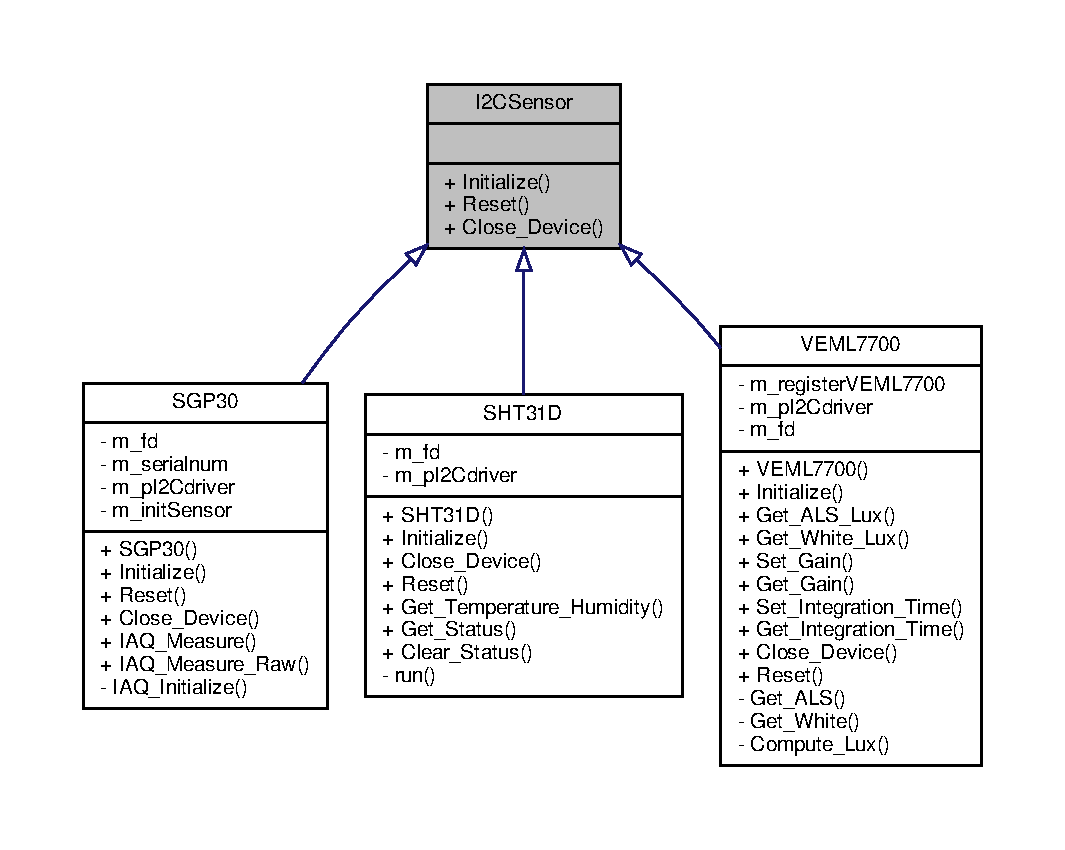
\includegraphics[width=350pt]{classI2CSensor__inherit__graph}
\end{center}
\end{figure}


Collaboration diagram for I2\+C\+Sensor\+:\nopagebreak
\begin{figure}[H]
\begin{center}
\leavevmode
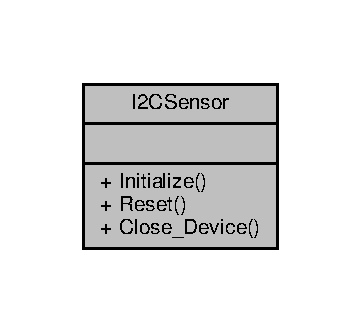
\includegraphics[width=173pt]{classI2CSensor__coll__graph}
\end{center}
\end{figure}
\subsection*{Public Member Functions}
\begin{DoxyCompactItemize}
\item 
virtual int \hyperlink{classI2CSensor_a0fb4755ddff3fe2cf5a9651d9d1fe5cd}{Initialize} (\hyperlink{classI2CDriver}{I2\+C\+Driver} \&i2c)=0
\item 
virtual int \hyperlink{classI2CSensor_a0622266d335944782d2bfa6352f01095}{Reset} ()=0
\item 
virtual int \hyperlink{classI2CSensor_acee1633439e97bae412441ac085fabba}{Close\+\_\+\+Device} ()=0
\end{DoxyCompactItemize}


\subsection{Detailed Description}
Generic Sensor Class which implements function for peripherial. 

\subsection{Member Function Documentation}
\mbox{\Hypertarget{classI2CSensor_acee1633439e97bae412441ac085fabba}\label{classI2CSensor_acee1633439e97bae412441ac085fabba}} 
\index{I2\+C\+Sensor@{I2\+C\+Sensor}!Close\+\_\+\+Device@{Close\+\_\+\+Device}}
\index{Close\+\_\+\+Device@{Close\+\_\+\+Device}!I2\+C\+Sensor@{I2\+C\+Sensor}}
\subsubsection{\texorpdfstring{Close\+\_\+\+Device()}{Close\_Device()}}
{\footnotesize\ttfamily virtual int I2\+C\+Sensor\+::\+Close\+\_\+\+Device (\begin{DoxyParamCaption}{ }\end{DoxyParamCaption})\hspace{0.3cm}{\ttfamily [pure virtual]}}

Read Data from the sensor and Reset Sensor Close File Descriptor 

Implemented in \hyperlink{classVEML7700_af4be747d3c60af76ca46c7e4fb859ec7}{V\+E\+M\+L7700}, \hyperlink{classSHT31D_a925cd964b0a6535d40dff588ac7d02be}{S\+H\+T31D}, and \hyperlink{classSGP30_a3feaf2623eb853169d14687e7ad1db24}{S\+G\+P30}.

\mbox{\Hypertarget{classI2CSensor_a0fb4755ddff3fe2cf5a9651d9d1fe5cd}\label{classI2CSensor_a0fb4755ddff3fe2cf5a9651d9d1fe5cd}} 
\index{I2\+C\+Sensor@{I2\+C\+Sensor}!Initialize@{Initialize}}
\index{Initialize@{Initialize}!I2\+C\+Sensor@{I2\+C\+Sensor}}
\subsubsection{\texorpdfstring{Initialize()}{Initialize()}}
{\footnotesize\ttfamily virtual int I2\+C\+Sensor\+::\+Initialize (\begin{DoxyParamCaption}\item[{\hyperlink{classI2CDriver}{I2\+C\+Driver} \&}]{i2c }\end{DoxyParamCaption})\hspace{0.3cm}{\ttfamily [pure virtual]}}

Initialize sensor Assign I2C Driver Open file descriptor Initial write to sensor to set it up using appropriate driver 

Implemented in \hyperlink{classVEML7700_af772ec5fe2bac04428479c9d232f1799}{V\+E\+M\+L7700}, \hyperlink{classSHT31D_af3ec39a4f04344a1b422761cc904343e}{S\+H\+T31D}, and \hyperlink{classSGP30_ad34fe8539ef007f55a0b3140889fdd6f}{S\+G\+P30}.

\mbox{\Hypertarget{classI2CSensor_a0622266d335944782d2bfa6352f01095}\label{classI2CSensor_a0622266d335944782d2bfa6352f01095}} 
\index{I2\+C\+Sensor@{I2\+C\+Sensor}!Reset@{Reset}}
\index{Reset@{Reset}!I2\+C\+Sensor@{I2\+C\+Sensor}}
\subsubsection{\texorpdfstring{Reset()}{Reset()}}
{\footnotesize\ttfamily virtual int I2\+C\+Sensor\+::\+Reset (\begin{DoxyParamCaption}{ }\end{DoxyParamCaption})\hspace{0.3cm}{\ttfamily [pure virtual]}}

Resets the sensor 

Implemented in \hyperlink{classVEML7700_a381358f8998260f4600a0d6713f7ea2a}{V\+E\+M\+L7700}, \hyperlink{classSHT31D_aa5d28c2557ed05435ca9b433492b9b07}{S\+H\+T31D}, and \hyperlink{classSGP30_a4934ef3a64eb0782a6d956c6526e4186}{S\+G\+P30}.



The documentation for this class was generated from the following file\+:\begin{DoxyCompactItemize}
\item 
src/controller/peripherials/\hyperlink{I2CSensor_8h}{I2\+C\+Sensor.\+h}\end{DoxyCompactItemize}

\hypertarget{classRelayBoard}{}\section{Relay\+Board Class Reference}
\label{classRelayBoard}\index{Relay\+Board@{Relay\+Board}}


Relay Board class.  




{\ttfamily \#include $<$Relay\+Board.\+h$>$}



Collaboration diagram for Relay\+Board\+:\nopagebreak
\begin{figure}[H]
\begin{center}
\leavevmode
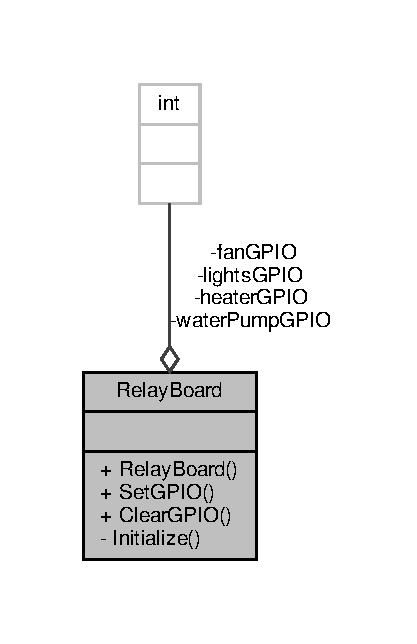
\includegraphics[width=213pt]{classRelayBoard__coll__graph}
\end{center}
\end{figure}
\subsection*{Public Member Functions}
\begin{DoxyCompactItemize}
\item 
\hyperlink{classRelayBoard_aa788c15cfc95188f5935f9d9d9fe86d2}{Relay\+Board} (void)
\item 
\hyperlink{classRelayBoard_af05bb34a287c76312104a427c86c658e}{$\sim$\+Relay\+Board} (void)
\item 
int \hyperlink{classRelayBoard_a161657ba51adff983bae66543ff5d365}{Set\+G\+P\+I\+O\+State} (int gpio\+Pin\+Number, int value)
\item 
int \hyperlink{classRelayBoard_a1011a5d79df5912e20d11053d7811ecd}{Set\+G\+P\+I\+O\+Direction} (int gpio\+Pin\+Number, int direction)
\item 
int \hyperlink{classRelayBoard_aced41245b932daad1709cc8d3b07bc4b}{G\+P\+I\+O\+Read} (int gpio\+Pin\+Number)
\item 
int \hyperlink{classRelayBoard_a501dbfa2878a57538eff31b16e70d74d}{Unexport\+G\+P\+IO} (int gpio\+Pin\+Number)
\item 
int \hyperlink{classRelayBoard_aa5394e9044c4271f9dcd9f08b9310b5b}{Export\+G\+P\+IO} (int gpio\+Pin\+Number)
\item 
int \hyperlink{classRelayBoard_a49759cb3cdcb6c2ccd7fbb44eb34b260}{Initialize} ()
\end{DoxyCompactItemize}
\subsection*{Private Member Functions}
\begin{DoxyCompactItemize}
\item 
int \hyperlink{classRelayBoard_a11b26e90f7a0831003a002937d28b30b}{Set\+Up\+Pin} (int gpio\+Pin\+Number)
\item 
int \hyperlink{classRelayBoard_aa63dcc275551dd06476c03d68a059228}{Unexport\+Pin} (int gpio\+Pin\+Number)
\item 
int \hyperlink{classRelayBoard_a83e2f4e38c382c0bf4a56d04640cfc27}{Close\+Device} ()
\end{DoxyCompactItemize}
\subsection*{Private Attributes}
\begin{DoxyCompactItemize}
\item 
int \hyperlink{classRelayBoard_a714832d9e7129960e0413b5618d2e310}{heater\+G\+P\+IO}
\item 
int \hyperlink{classRelayBoard_a05f68a6555288127a238e31282886ae0}{lights\+G\+P\+IO}
\item 
int \hyperlink{classRelayBoard_a0b33569569f2698b99a17e65f6dbc5a1}{lights\+G\+P\+I\+O\+State}
\item 
int \hyperlink{classRelayBoard_a70ab1391ffac8f4c01c64ba1a811b6fc}{fan\+G\+P\+IO}
\item 
int \hyperlink{classRelayBoard_a195c50d455165712f59cd39c6f7a6b82}{water\+Pump\+G\+P\+IO}
\end{DoxyCompactItemize}


\subsection{Detailed Description}
Relay Board class. 

\begin{DoxyAuthor}{Author}
Kamil Rog
\end{DoxyAuthor}
This is class is responsilbe for the Elego Relay Board. 

\subsection{Constructor \& Destructor Documentation}
\mbox{\Hypertarget{classRelayBoard_aa788c15cfc95188f5935f9d9d9fe86d2}\label{classRelayBoard_aa788c15cfc95188f5935f9d9d9fe86d2}} 
\index{Relay\+Board@{Relay\+Board}!Relay\+Board@{Relay\+Board}}
\index{Relay\+Board@{Relay\+Board}!Relay\+Board@{Relay\+Board}}
\subsubsection{\texorpdfstring{Relay\+Board()}{RelayBoard()}}
{\footnotesize\ttfamily Relay\+Board\+::\+Relay\+Board (\begin{DoxyParamCaption}\item[{void}]{ }\end{DoxyParamCaption})\hspace{0.3cm}{\ttfamily [inline]}}

\mbox{\Hypertarget{classRelayBoard_af05bb34a287c76312104a427c86c658e}\label{classRelayBoard_af05bb34a287c76312104a427c86c658e}} 
\index{Relay\+Board@{Relay\+Board}!````~Relay\+Board@{$\sim$\+Relay\+Board}}
\index{````~Relay\+Board@{$\sim$\+Relay\+Board}!Relay\+Board@{Relay\+Board}}
\subsubsection{\texorpdfstring{$\sim$\+Relay\+Board()}{~RelayBoard()}}
{\footnotesize\ttfamily Relay\+Board\+::$\sim$\+Relay\+Board (\begin{DoxyParamCaption}\item[{void}]{ }\end{DoxyParamCaption})\hspace{0.3cm}{\ttfamily [inline]}}



\subsection{Member Function Documentation}
\mbox{\Hypertarget{classRelayBoard_a83e2f4e38c382c0bf4a56d04640cfc27}\label{classRelayBoard_a83e2f4e38c382c0bf4a56d04640cfc27}} 
\index{Relay\+Board@{Relay\+Board}!Close\+Device@{Close\+Device}}
\index{Close\+Device@{Close\+Device}!Relay\+Board@{Relay\+Board}}
\subsubsection{\texorpdfstring{Close\+Device()}{CloseDevice()}}
{\footnotesize\ttfamily int Relay\+Board\+::\+Close\+Device (\begin{DoxyParamCaption}{ }\end{DoxyParamCaption})\hspace{0.3cm}{\ttfamily [private]}}

\mbox{\Hypertarget{classRelayBoard_aa5394e9044c4271f9dcd9f08b9310b5b}\label{classRelayBoard_aa5394e9044c4271f9dcd9f08b9310b5b}} 
\index{Relay\+Board@{Relay\+Board}!Export\+G\+P\+IO@{Export\+G\+P\+IO}}
\index{Export\+G\+P\+IO@{Export\+G\+P\+IO}!Relay\+Board@{Relay\+Board}}
\subsubsection{\texorpdfstring{Export\+G\+P\+I\+O()}{ExportGPIO()}}
{\footnotesize\ttfamily int Relay\+Board\+::\+Export\+G\+P\+IO (\begin{DoxyParamCaption}\item[{int}]{gpio\+Pin\+Number }\end{DoxyParamCaption})}

\mbox{\Hypertarget{classRelayBoard_aced41245b932daad1709cc8d3b07bc4b}\label{classRelayBoard_aced41245b932daad1709cc8d3b07bc4b}} 
\index{Relay\+Board@{Relay\+Board}!G\+P\+I\+O\+Read@{G\+P\+I\+O\+Read}}
\index{G\+P\+I\+O\+Read@{G\+P\+I\+O\+Read}!Relay\+Board@{Relay\+Board}}
\subsubsection{\texorpdfstring{G\+P\+I\+O\+Read()}{GPIORead()}}
{\footnotesize\ttfamily int Relay\+Board\+::\+G\+P\+I\+O\+Read (\begin{DoxyParamCaption}\item[{int}]{gpio\+Pin\+Number }\end{DoxyParamCaption})}

\mbox{\Hypertarget{classRelayBoard_a49759cb3cdcb6c2ccd7fbb44eb34b260}\label{classRelayBoard_a49759cb3cdcb6c2ccd7fbb44eb34b260}} 
\index{Relay\+Board@{Relay\+Board}!Initialize@{Initialize}}
\index{Initialize@{Initialize}!Relay\+Board@{Relay\+Board}}
\subsubsection{\texorpdfstring{Initialize()}{Initialize()}}
{\footnotesize\ttfamily int Relay\+Board\+::\+Initialize (\begin{DoxyParamCaption}{ }\end{DoxyParamCaption})}

\mbox{\Hypertarget{classRelayBoard_a1011a5d79df5912e20d11053d7811ecd}\label{classRelayBoard_a1011a5d79df5912e20d11053d7811ecd}} 
\index{Relay\+Board@{Relay\+Board}!Set\+G\+P\+I\+O\+Direction@{Set\+G\+P\+I\+O\+Direction}}
\index{Set\+G\+P\+I\+O\+Direction@{Set\+G\+P\+I\+O\+Direction}!Relay\+Board@{Relay\+Board}}
\subsubsection{\texorpdfstring{Set\+G\+P\+I\+O\+Direction()}{SetGPIODirection()}}
{\footnotesize\ttfamily int Relay\+Board\+::\+Set\+G\+P\+I\+O\+Direction (\begin{DoxyParamCaption}\item[{int}]{gpio\+Pin\+Number,  }\item[{int}]{direction }\end{DoxyParamCaption})}

\mbox{\Hypertarget{classRelayBoard_a161657ba51adff983bae66543ff5d365}\label{classRelayBoard_a161657ba51adff983bae66543ff5d365}} 
\index{Relay\+Board@{Relay\+Board}!Set\+G\+P\+I\+O\+State@{Set\+G\+P\+I\+O\+State}}
\index{Set\+G\+P\+I\+O\+State@{Set\+G\+P\+I\+O\+State}!Relay\+Board@{Relay\+Board}}
\subsubsection{\texorpdfstring{Set\+G\+P\+I\+O\+State()}{SetGPIOState()}}
{\footnotesize\ttfamily int Relay\+Board\+::\+Set\+G\+P\+I\+O\+State (\begin{DoxyParamCaption}\item[{int}]{gpio\+Pin\+Number,  }\item[{int}]{value }\end{DoxyParamCaption})}

\mbox{\Hypertarget{classRelayBoard_a11b26e90f7a0831003a002937d28b30b}\label{classRelayBoard_a11b26e90f7a0831003a002937d28b30b}} 
\index{Relay\+Board@{Relay\+Board}!Set\+Up\+Pin@{Set\+Up\+Pin}}
\index{Set\+Up\+Pin@{Set\+Up\+Pin}!Relay\+Board@{Relay\+Board}}
\subsubsection{\texorpdfstring{Set\+Up\+Pin()}{SetUpPin()}}
{\footnotesize\ttfamily int Relay\+Board\+::\+Set\+Up\+Pin (\begin{DoxyParamCaption}\item[{int}]{gpio\+Pin\+Number }\end{DoxyParamCaption})\hspace{0.3cm}{\ttfamily [private]}}

Initialize G\+P\+IO Pins for using Relay Board.

\begin{DoxyReturn}{Returns}
Zero on success error 
\end{DoxyReturn}
\mbox{\Hypertarget{classRelayBoard_a501dbfa2878a57538eff31b16e70d74d}\label{classRelayBoard_a501dbfa2878a57538eff31b16e70d74d}} 
\index{Relay\+Board@{Relay\+Board}!Unexport\+G\+P\+IO@{Unexport\+G\+P\+IO}}
\index{Unexport\+G\+P\+IO@{Unexport\+G\+P\+IO}!Relay\+Board@{Relay\+Board}}
\subsubsection{\texorpdfstring{Unexport\+G\+P\+I\+O()}{UnexportGPIO()}}
{\footnotesize\ttfamily int Relay\+Board\+::\+Unexport\+G\+P\+IO (\begin{DoxyParamCaption}\item[{int}]{gpio\+Pin\+Number }\end{DoxyParamCaption})}

\mbox{\Hypertarget{classRelayBoard_aa63dcc275551dd06476c03d68a059228}\label{classRelayBoard_aa63dcc275551dd06476c03d68a059228}} 
\index{Relay\+Board@{Relay\+Board}!Unexport\+Pin@{Unexport\+Pin}}
\index{Unexport\+Pin@{Unexport\+Pin}!Relay\+Board@{Relay\+Board}}
\subsubsection{\texorpdfstring{Unexport\+Pin()}{UnexportPin()}}
{\footnotesize\ttfamily int Relay\+Board\+::\+Unexport\+Pin (\begin{DoxyParamCaption}\item[{int}]{gpio\+Pin\+Number }\end{DoxyParamCaption})\hspace{0.3cm}{\ttfamily [private]}}



\subsection{Member Data Documentation}
\mbox{\Hypertarget{classRelayBoard_a70ab1391ffac8f4c01c64ba1a811b6fc}\label{classRelayBoard_a70ab1391ffac8f4c01c64ba1a811b6fc}} 
\index{Relay\+Board@{Relay\+Board}!fan\+G\+P\+IO@{fan\+G\+P\+IO}}
\index{fan\+G\+P\+IO@{fan\+G\+P\+IO}!Relay\+Board@{Relay\+Board}}
\subsubsection{\texorpdfstring{fan\+G\+P\+IO}{fanGPIO}}
{\footnotesize\ttfamily int Relay\+Board\+::fan\+G\+P\+IO\hspace{0.3cm}{\ttfamily [private]}}

\mbox{\Hypertarget{classRelayBoard_a714832d9e7129960e0413b5618d2e310}\label{classRelayBoard_a714832d9e7129960e0413b5618d2e310}} 
\index{Relay\+Board@{Relay\+Board}!heater\+G\+P\+IO@{heater\+G\+P\+IO}}
\index{heater\+G\+P\+IO@{heater\+G\+P\+IO}!Relay\+Board@{Relay\+Board}}
\subsubsection{\texorpdfstring{heater\+G\+P\+IO}{heaterGPIO}}
{\footnotesize\ttfamily int Relay\+Board\+::heater\+G\+P\+IO\hspace{0.3cm}{\ttfamily [private]}}

\mbox{\Hypertarget{classRelayBoard_a05f68a6555288127a238e31282886ae0}\label{classRelayBoard_a05f68a6555288127a238e31282886ae0}} 
\index{Relay\+Board@{Relay\+Board}!lights\+G\+P\+IO@{lights\+G\+P\+IO}}
\index{lights\+G\+P\+IO@{lights\+G\+P\+IO}!Relay\+Board@{Relay\+Board}}
\subsubsection{\texorpdfstring{lights\+G\+P\+IO}{lightsGPIO}}
{\footnotesize\ttfamily int Relay\+Board\+::lights\+G\+P\+IO\hspace{0.3cm}{\ttfamily [private]}}

\mbox{\Hypertarget{classRelayBoard_a0b33569569f2698b99a17e65f6dbc5a1}\label{classRelayBoard_a0b33569569f2698b99a17e65f6dbc5a1}} 
\index{Relay\+Board@{Relay\+Board}!lights\+G\+P\+I\+O\+State@{lights\+G\+P\+I\+O\+State}}
\index{lights\+G\+P\+I\+O\+State@{lights\+G\+P\+I\+O\+State}!Relay\+Board@{Relay\+Board}}
\subsubsection{\texorpdfstring{lights\+G\+P\+I\+O\+State}{lightsGPIOState}}
{\footnotesize\ttfamily int Relay\+Board\+::lights\+G\+P\+I\+O\+State\hspace{0.3cm}{\ttfamily [private]}}

\mbox{\Hypertarget{classRelayBoard_a195c50d455165712f59cd39c6f7a6b82}\label{classRelayBoard_a195c50d455165712f59cd39c6f7a6b82}} 
\index{Relay\+Board@{Relay\+Board}!water\+Pump\+G\+P\+IO@{water\+Pump\+G\+P\+IO}}
\index{water\+Pump\+G\+P\+IO@{water\+Pump\+G\+P\+IO}!Relay\+Board@{Relay\+Board}}
\subsubsection{\texorpdfstring{water\+Pump\+G\+P\+IO}{waterPumpGPIO}}
{\footnotesize\ttfamily int Relay\+Board\+::water\+Pump\+G\+P\+IO\hspace{0.3cm}{\ttfamily [private]}}



The documentation for this class was generated from the following files\+:\begin{DoxyCompactItemize}
\item 
src/controller/peripherials/\hyperlink{RelayBoard_8h}{Relay\+Board.\+h}\item 
src/controller/peripherials/\hyperlink{RelayBoard_8cpp}{Relay\+Board.\+cpp}\end{DoxyCompactItemize}

\hypertarget{classCppTimerCallback_1_1Runnable}{}\section{Cpp\+Timer\+Callback\+:\+:Runnable Class Reference}
\label{classCppTimerCallback_1_1Runnable}\index{Cpp\+Timer\+Callback\+::\+Runnable@{Cpp\+Timer\+Callback\+::\+Runnable}}


{\ttfamily \#include $<$Cpp\+Timer\+Callback.\+h$>$}



Collaboration diagram for Cpp\+Timer\+Callback\+:\+:Runnable\+:\nopagebreak
\begin{figure}[H]
\begin{center}
\leavevmode
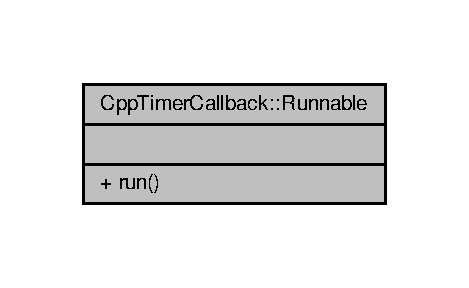
\includegraphics[width=225pt]{classCppTimerCallback_1_1Runnable__coll__graph}
\end{center}
\end{figure}
\subsection*{Public Member Functions}
\begin{DoxyCompactItemize}
\item 
virtual void \hyperlink{classCppTimerCallback_1_1Runnable_af8d11a3b580e76431151e76ac1886e6e}{run} ()=0
\end{DoxyCompactItemize}


\subsection{Member Function Documentation}
\mbox{\Hypertarget{classCppTimerCallback_1_1Runnable_af8d11a3b580e76431151e76ac1886e6e}\label{classCppTimerCallback_1_1Runnable_af8d11a3b580e76431151e76ac1886e6e}} 
\index{Cpp\+Timer\+Callback\+::\+Runnable@{Cpp\+Timer\+Callback\+::\+Runnable}!run@{run}}
\index{run@{run}!Cpp\+Timer\+Callback\+::\+Runnable@{Cpp\+Timer\+Callback\+::\+Runnable}}
\subsubsection{\texorpdfstring{run()}{run()}}
{\footnotesize\ttfamily virtual void Cpp\+Timer\+Callback\+::\+Runnable\+::run (\begin{DoxyParamCaption}{ }\end{DoxyParamCaption})\hspace{0.3cm}{\ttfamily [pure virtual]}}



The documentation for this class was generated from the following file\+:\begin{DoxyCompactItemize}
\item 
src/utils/\hyperlink{CppTimerCallback_8h}{Cpp\+Timer\+Callback.\+h}\end{DoxyCompactItemize}

\hypertarget{classSampler}{}\section{Sampler Class Reference}
\label{classSampler}\index{Sampler@{Sampler}}


\hyperlink{classSampler}{Sampler} Class.  




{\ttfamily \#include $<$Sampler.\+h$>$}



Inheritance diagram for Sampler\+:
\nopagebreak
\begin{figure}[H]
\begin{center}
\leavevmode
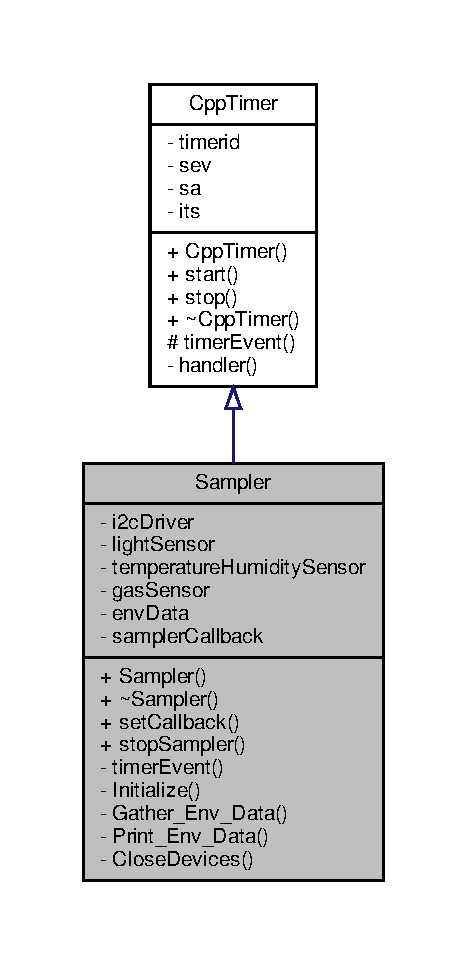
\includegraphics[width=224pt]{classSampler__inherit__graph}
\end{center}
\end{figure}


Collaboration diagram for Sampler\+:
\nopagebreak
\begin{figure}[H]
\begin{center}
\leavevmode
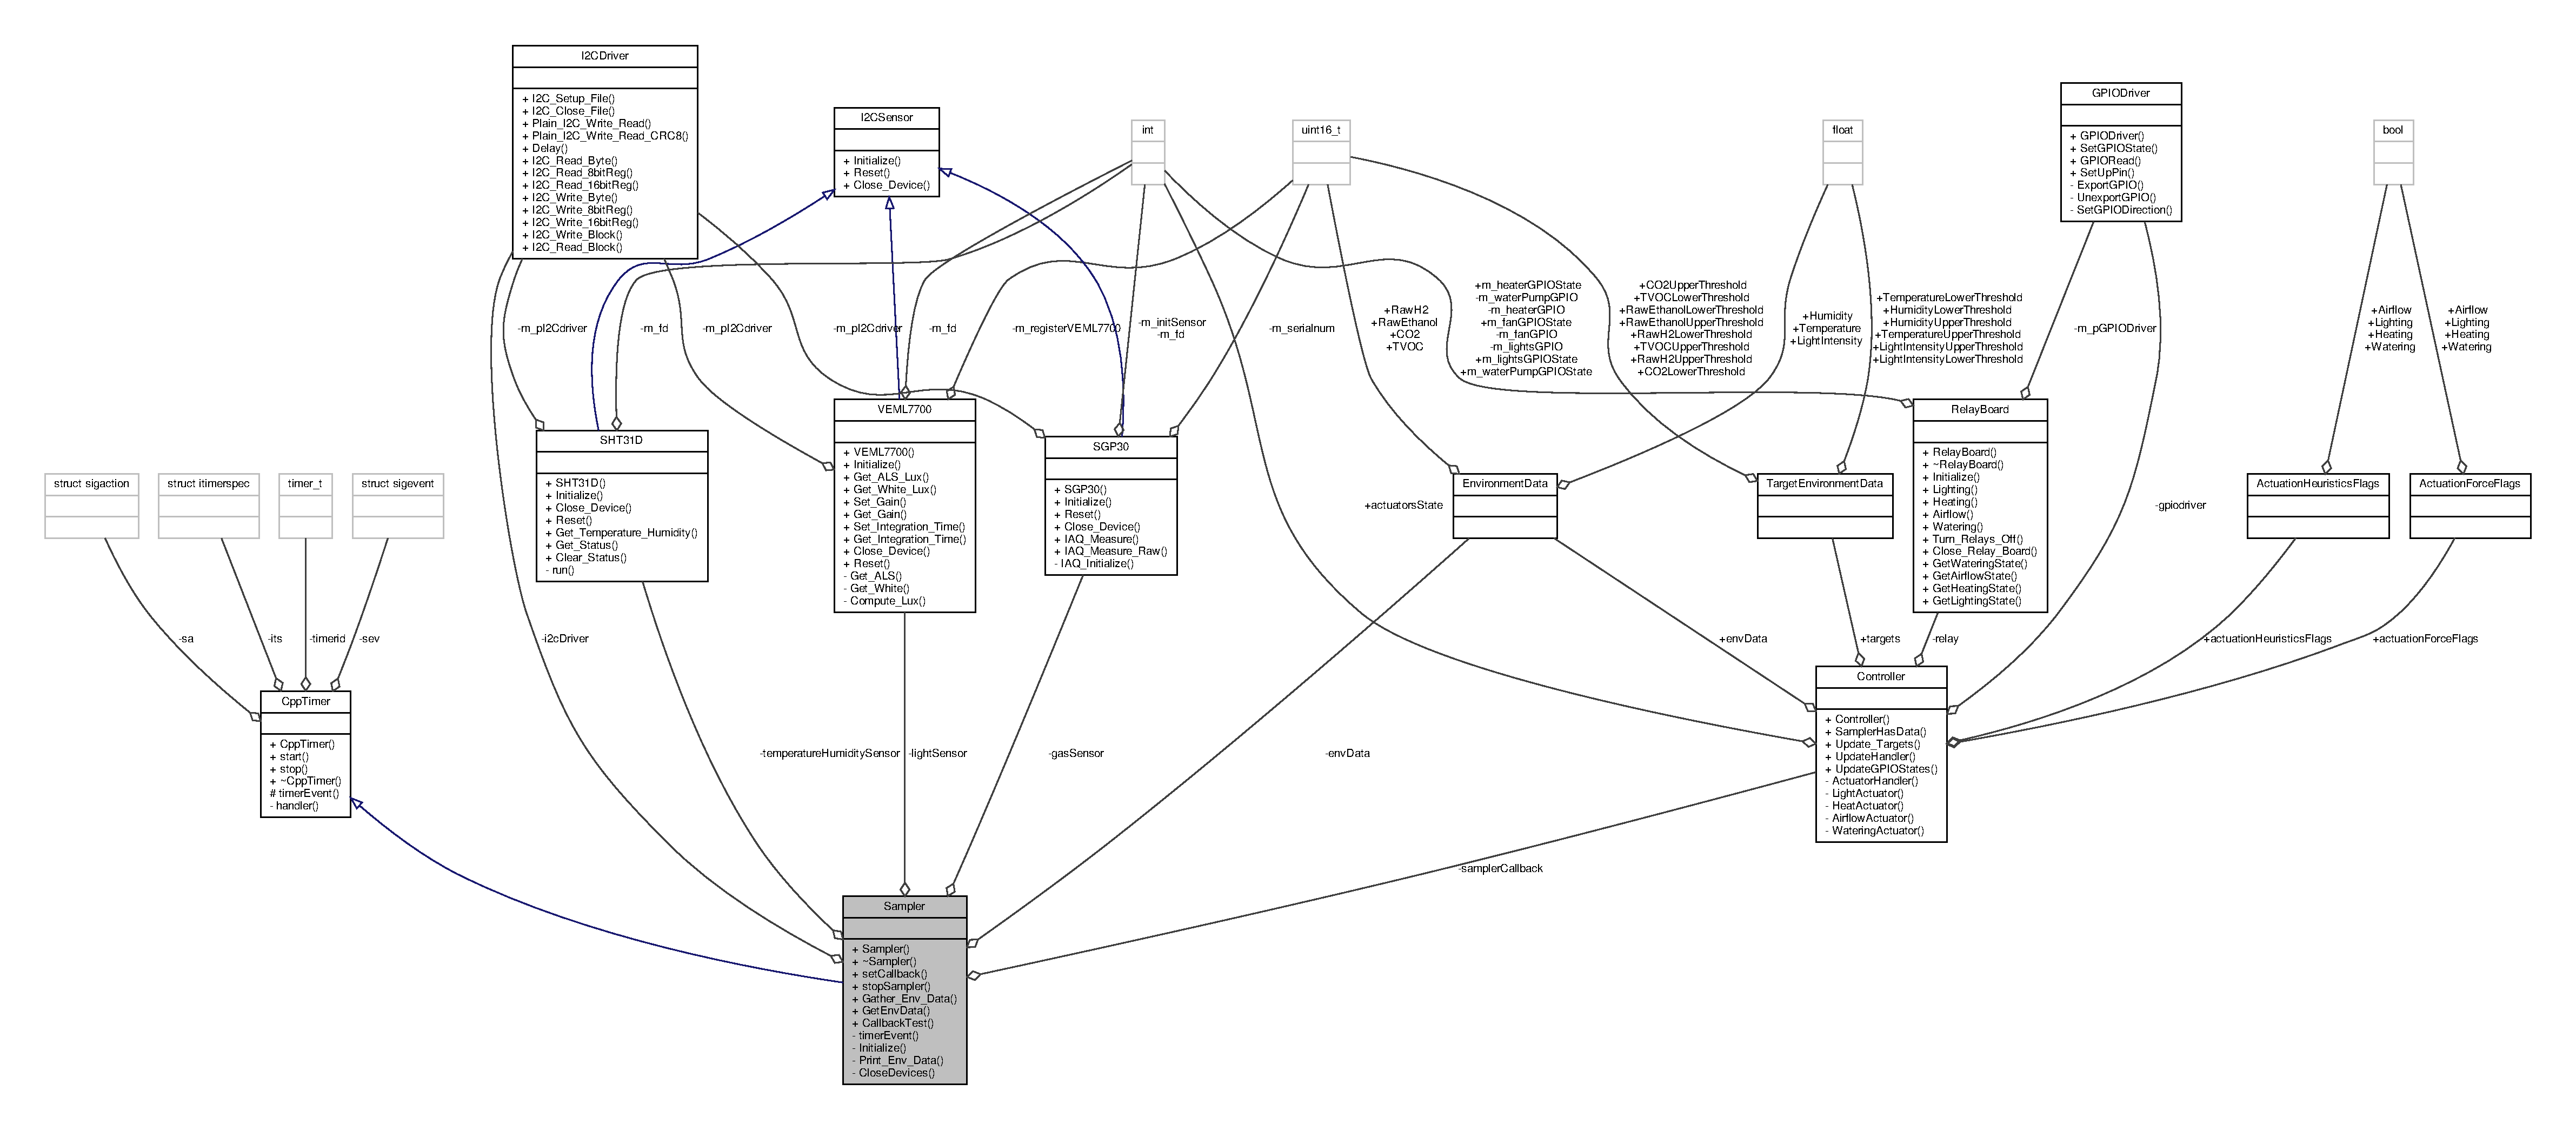
\includegraphics[width=350pt]{classSampler__coll__graph}
\end{center}
\end{figure}
\subsection*{Public Member Functions}
\begin{DoxyCompactItemize}
\item 
\hyperlink{classSampler_aec4905ed5f8259bb5e361da172bf7f17}{Sampler} (\hyperlink{classController}{Controller} $\ast$cb)
\item 
\hyperlink{classSampler_afbbbd238b78dd3024686c852b69fa64e}{$\sim$\+Sampler} ()
\begin{DoxyCompactList}\small\item\em Destructor. \end{DoxyCompactList}\item 
void \hyperlink{classSampler_a026a0839919e8e93fa75f19b67ccffc6}{set\+Callback} (\hyperlink{classController}{Controller} $\ast$cb)
\item 
void \hyperlink{classSampler_af661f48134a6d0f1f2d6080f5025392e}{stop\+Sampler} ()
\item 
int \hyperlink{classSampler_a5702d0ef89adb532fef4f9879e7e36d4}{Gather\+\_\+\+Env\+\_\+\+Data} ()
\begin{DoxyCompactList}\small\item\em Test Functions. \end{DoxyCompactList}\item 
\hyperlink{structEnvironmentData}{Environment\+Data} \hyperlink{classSampler_a22edd729c6bbb5582ebac7681041cf55}{Get\+Env\+Data} ()
\item 
void \hyperlink{classSampler_a4e239960ef9947af152ba441ba152cd0}{Callback\+Test} ()
\item 
virtual void \hyperlink{classCppTimer_a64989025caa3c030c6c397ca76a2d20b}{start} (long nanosecs, \hyperlink{CppTimer_8h_a110d07ab6a96d7815149d3d95435790a}{cpp\+Timer\+Type\+\_\+t} type=\hyperlink{CppTimer_8h_a110d07ab6a96d7815149d3d95435790aae4379d044711537d9ce3b3b58c575c58}{P\+E\+R\+I\+O\+D\+IC})
\item 
virtual void \hyperlink{classCppTimer_a4bb95ddee98a536d0818b8f6096bf7e7}{stop} ()
\end{DoxyCompactItemize}
\subsection*{Private Member Functions}
\begin{DoxyCompactItemize}
\item 
void \hyperlink{classSampler_addf333c6e247ee3a1def41260caa902a}{timer\+Event} ()
\item 
int \hyperlink{classSampler_a1aed5b32bf99312ba38d092f1acad3d9}{Initialize} ()
\item 
int \hyperlink{classSampler_acf3d04a740356e54fe53766a7f00ae15}{Print\+\_\+\+Env\+\_\+\+Data} ()
\item 
int \hyperlink{classSampler_a24077f1eeb2491b65f9577efd07dffd6}{Close\+Devices} ()
\end{DoxyCompactItemize}
\subsection*{Private Attributes}
\begin{DoxyCompactItemize}
\item 
\hyperlink{classI2CDriver}{I2\+C\+Driver} \hyperlink{classSampler_ada5598060be79a005bf4375fcbf9773d}{i2c\+Driver}
\begin{DoxyCompactList}\small\item\em I2C driver used for. \end{DoxyCompactList}\item 
\hyperlink{classVEML7700}{V\+E\+M\+L7700} \hyperlink{classSampler_ae81394f464670af514f8dc7c5df46d74}{light\+Sensor}
\begin{DoxyCompactList}\small\item\em Peripherials using I2C driver -\/ instantiate new sensors here. \end{DoxyCompactList}\item 
\hyperlink{classSHT31D}{S\+H\+T31D} \hyperlink{classSampler_aad073931f59004109e8050c669b294c0}{temperature\+Humidity\+Sensor}
\item 
\hyperlink{classSGP30}{S\+G\+P30} \hyperlink{classSampler_a4af78e46617fc8cdbc4bd14a7db5c741}{gas\+Sensor}
\item 
\hyperlink{structEnvironmentData}{Environment\+Data} \hyperlink{classSampler_a4cfbeb66e1cd18cfc66ccdb2712770f9}{env\+Data}
\begin{DoxyCompactList}\small\item\em Current and Target Enviroment Data Struct. \end{DoxyCompactList}\item 
\hyperlink{classController}{Controller} $\ast$ \hyperlink{classSampler_a3a37b5d667134d905e4bda45974cb936}{sampler\+Callback} = nullptr
\begin{DoxyCompactList}\small\item\em Pointer to conroller object. \end{DoxyCompactList}\end{DoxyCompactItemize}


\subsection{Detailed Description}
\hyperlink{classSampler}{Sampler} Class. 

\begin{DoxyAuthor}{Author}
Kamil Rog
\end{DoxyAuthor}
This class is responsible for taking measurements for all devices on I2C Bus. This is achiebed by inheriting functionality of \hyperlink{classCppTimer}{Cpp\+Timer}. \hyperlink{classSampler_addf333c6e247ee3a1def41260caa902a}{timer\+Event()} is executed when timer fires. This sampler creates new thread 

\subsection{Constructor \& Destructor Documentation}
\mbox{\Hypertarget{classSampler_aec4905ed5f8259bb5e361da172bf7f17}\label{classSampler_aec4905ed5f8259bb5e361da172bf7f17}} 
\index{Sampler@{Sampler}!Sampler@{Sampler}}
\index{Sampler@{Sampler}!Sampler@{Sampler}}
\subsubsection{\texorpdfstring{Sampler()}{Sampler()}}
{\footnotesize\ttfamily Sampler\+::\+Sampler (\begin{DoxyParamCaption}\item[{\hyperlink{classController}{Controller} $\ast$}]{cb }\end{DoxyParamCaption})\hspace{0.3cm}{\ttfamily [inline]}}

\mbox{\Hypertarget{classSampler_afbbbd238b78dd3024686c852b69fa64e}\label{classSampler_afbbbd238b78dd3024686c852b69fa64e}} 
\index{Sampler@{Sampler}!````~Sampler@{$\sim$\+Sampler}}
\index{````~Sampler@{$\sim$\+Sampler}!Sampler@{Sampler}}
\subsubsection{\texorpdfstring{$\sim$\+Sampler()}{~Sampler()}}
{\footnotesize\ttfamily Sampler\+::$\sim$\+Sampler (\begin{DoxyParamCaption}{ }\end{DoxyParamCaption})\hspace{0.3cm}{\ttfamily [inline]}}



Destructor. 



\subsection{Member Function Documentation}
\mbox{\Hypertarget{classSampler_a4e239960ef9947af152ba441ba152cd0}\label{classSampler_a4e239960ef9947af152ba441ba152cd0}} 
\index{Sampler@{Sampler}!Callback\+Test@{Callback\+Test}}
\index{Callback\+Test@{Callback\+Test}!Sampler@{Sampler}}
\subsubsection{\texorpdfstring{Callback\+Test()}{CallbackTest()}}
{\footnotesize\ttfamily void Sampler\+::\+Callback\+Test (\begin{DoxyParamCaption}{ }\end{DoxyParamCaption})}

Use Callback Currently used only for integation test \mbox{\Hypertarget{classSampler_a24077f1eeb2491b65f9577efd07dffd6}\label{classSampler_a24077f1eeb2491b65f9577efd07dffd6}} 
\index{Sampler@{Sampler}!Close\+Devices@{Close\+Devices}}
\index{Close\+Devices@{Close\+Devices}!Sampler@{Sampler}}
\subsubsection{\texorpdfstring{Close\+Devices()}{CloseDevices()}}
{\footnotesize\ttfamily int Sampler\+::\+Close\+Devices (\begin{DoxyParamCaption}{ }\end{DoxyParamCaption})\hspace{0.3cm}{\ttfamily [private]}}

Closes each I2C measurement device by turn.

\begin{DoxyReturn}{Returns}
Zero On Sucess 
\end{DoxyReturn}
\mbox{\Hypertarget{classSampler_a5702d0ef89adb532fef4f9879e7e36d4}\label{classSampler_a5702d0ef89adb532fef4f9879e7e36d4}} 
\index{Sampler@{Sampler}!Gather\+\_\+\+Env\+\_\+\+Data@{Gather\+\_\+\+Env\+\_\+\+Data}}
\index{Gather\+\_\+\+Env\+\_\+\+Data@{Gather\+\_\+\+Env\+\_\+\+Data}!Sampler@{Sampler}}
\subsubsection{\texorpdfstring{Gather\+\_\+\+Env\+\_\+\+Data()}{Gather\_Env\_Data()}}
{\footnotesize\ttfamily int Sampler\+::\+Gather\+\_\+\+Env\+\_\+\+Data (\begin{DoxyParamCaption}{ }\end{DoxyParamCaption})}



Test Functions. 

Reads data from all sensors by turn.

\begin{DoxyReturn}{Returns}
Zero On Sucess 
\end{DoxyReturn}
\mbox{\Hypertarget{classSampler_a22edd729c6bbb5582ebac7681041cf55}\label{classSampler_a22edd729c6bbb5582ebac7681041cf55}} 
\index{Sampler@{Sampler}!Get\+Env\+Data@{Get\+Env\+Data}}
\index{Get\+Env\+Data@{Get\+Env\+Data}!Sampler@{Sampler}}
\subsubsection{\texorpdfstring{Get\+Env\+Data()}{GetEnvData()}}
{\footnotesize\ttfamily \hyperlink{structEnvironmentData}{Environment\+Data} Sampler\+::\+Get\+Env\+Data (\begin{DoxyParamCaption}{ }\end{DoxyParamCaption})}

Returns the current data from all sensors by turn. Currently used only for integation tests

\begin{DoxyReturn}{Returns}
Environment data struct 
\end{DoxyReturn}
\mbox{\Hypertarget{classSampler_a1aed5b32bf99312ba38d092f1acad3d9}\label{classSampler_a1aed5b32bf99312ba38d092f1acad3d9}} 
\index{Sampler@{Sampler}!Initialize@{Initialize}}
\index{Initialize@{Initialize}!Sampler@{Sampler}}
\subsubsection{\texorpdfstring{Initialize()}{Initialize()}}
{\footnotesize\ttfamily int Sampler\+::\+Initialize (\begin{DoxyParamCaption}{ }\end{DoxyParamCaption})\hspace{0.3cm}{\ttfamily [private]}}

Initialize all enviromental data struct variables and sensors.

filepath filepath for settings file. \mbox{\Hypertarget{classSampler_acf3d04a740356e54fe53766a7f00ae15}\label{classSampler_acf3d04a740356e54fe53766a7f00ae15}} 
\index{Sampler@{Sampler}!Print\+\_\+\+Env\+\_\+\+Data@{Print\+\_\+\+Env\+\_\+\+Data}}
\index{Print\+\_\+\+Env\+\_\+\+Data@{Print\+\_\+\+Env\+\_\+\+Data}!Sampler@{Sampler}}
\subsubsection{\texorpdfstring{Print\+\_\+\+Env\+\_\+\+Data()}{Print\_Env\_Data()}}
{\footnotesize\ttfamily int Sampler\+::\+Print\+\_\+\+Env\+\_\+\+Data (\begin{DoxyParamCaption}{ }\end{DoxyParamCaption})\hspace{0.3cm}{\ttfamily [private]}}

Prints data read by sensors by turn.

\begin{DoxyReturn}{Returns}
Zero On Sucess 
\end{DoxyReturn}
\mbox{\Hypertarget{classSampler_a026a0839919e8e93fa75f19b67ccffc6}\label{classSampler_a026a0839919e8e93fa75f19b67ccffc6}} 
\index{Sampler@{Sampler}!set\+Callback@{set\+Callback}}
\index{set\+Callback@{set\+Callback}!Sampler@{Sampler}}
\subsubsection{\texorpdfstring{set\+Callback()}{setCallback()}}
{\footnotesize\ttfamily void Sampler\+::set\+Callback (\begin{DoxyParamCaption}\item[{\hyperlink{classController}{Controller} $\ast$}]{cb }\end{DoxyParamCaption})\hspace{0.3cm}{\ttfamily [inline]}}

Sets the callback which is called whenever there is new data \mbox{\Hypertarget{classCppTimer_a64989025caa3c030c6c397ca76a2d20b}\label{classCppTimer_a64989025caa3c030c6c397ca76a2d20b}} 
\index{Sampler@{Sampler}!start@{start}}
\index{start@{start}!Sampler@{Sampler}}
\subsubsection{\texorpdfstring{start()}{start()}}
{\footnotesize\ttfamily void Cpp\+Timer\+::start (\begin{DoxyParamCaption}\item[{long}]{nanosecs,  }\item[{\hyperlink{CppTimer_8h_a110d07ab6a96d7815149d3d95435790a}{cpp\+Timer\+Type\+\_\+t}}]{type = {\ttfamily \hyperlink{CppTimer_8h_a110d07ab6a96d7815149d3d95435790aae4379d044711537d9ce3b3b58c575c58}{P\+E\+R\+I\+O\+D\+IC}} }\end{DoxyParamCaption})\hspace{0.3cm}{\ttfamily [virtual]}, {\ttfamily [inherited]}}

Starts the timer. The timer fires first after the specified time in nanoseconds and then at that interval in P\+E\+R\+I\+O\+D\+IC mode. In O\+N\+E\+S\+H\+OT mode the timer fires once after the specified time in nanoseconds. \mbox{\Hypertarget{classCppTimer_a4bb95ddee98a536d0818b8f6096bf7e7}\label{classCppTimer_a4bb95ddee98a536d0818b8f6096bf7e7}} 
\index{Sampler@{Sampler}!stop@{stop}}
\index{stop@{stop}!Sampler@{Sampler}}
\subsubsection{\texorpdfstring{stop()}{stop()}}
{\footnotesize\ttfamily void Cpp\+Timer\+::stop (\begin{DoxyParamCaption}{ }\end{DoxyParamCaption})\hspace{0.3cm}{\ttfamily [virtual]}, {\ttfamily [inherited]}}

Stops the timer by disarming it. It can be re-\/started with \hyperlink{classCppTimer_a64989025caa3c030c6c397ca76a2d20b}{start()}. \mbox{\Hypertarget{classSampler_af661f48134a6d0f1f2d6080f5025392e}\label{classSampler_af661f48134a6d0f1f2d6080f5025392e}} 
\index{Sampler@{Sampler}!stop\+Sampler@{stop\+Sampler}}
\index{stop\+Sampler@{stop\+Sampler}!Sampler@{Sampler}}
\subsubsection{\texorpdfstring{stop\+Sampler()}{stopSampler()}}
{\footnotesize\ttfamily void Sampler\+::stop\+Sampler (\begin{DoxyParamCaption}{ }\end{DoxyParamCaption})\hspace{0.3cm}{\ttfamily [inline]}}

Stops the data acquistion \mbox{\Hypertarget{classSampler_addf333c6e247ee3a1def41260caa902a}\label{classSampler_addf333c6e247ee3a1def41260caa902a}} 
\index{Sampler@{Sampler}!timer\+Event@{timer\+Event}}
\index{timer\+Event@{timer\+Event}!Sampler@{Sampler}}
\subsubsection{\texorpdfstring{timer\+Event()}{timerEvent()}}
{\footnotesize\ttfamily void Sampler\+::timer\+Event (\begin{DoxyParamCaption}{ }\end{DoxyParamCaption})\hspace{0.3cm}{\ttfamily [inline]}, {\ttfamily [private]}, {\ttfamily [virtual]}}

Executes when timer fires. Firstly it takes measurements and runs the callback function defined in the controller object 

Implements \hyperlink{classCppTimer_ac2665403595b6aee5f581d0ebfeb886c}{Cpp\+Timer}.



\subsection{Member Data Documentation}
\mbox{\Hypertarget{classSampler_a4cfbeb66e1cd18cfc66ccdb2712770f9}\label{classSampler_a4cfbeb66e1cd18cfc66ccdb2712770f9}} 
\index{Sampler@{Sampler}!env\+Data@{env\+Data}}
\index{env\+Data@{env\+Data}!Sampler@{Sampler}}
\subsubsection{\texorpdfstring{env\+Data}{envData}}
{\footnotesize\ttfamily \hyperlink{structEnvironmentData}{Environment\+Data} Sampler\+::env\+Data\hspace{0.3cm}{\ttfamily [private]}}



Current and Target Enviroment Data Struct. 

\mbox{\Hypertarget{classSampler_a4af78e46617fc8cdbc4bd14a7db5c741}\label{classSampler_a4af78e46617fc8cdbc4bd14a7db5c741}} 
\index{Sampler@{Sampler}!gas\+Sensor@{gas\+Sensor}}
\index{gas\+Sensor@{gas\+Sensor}!Sampler@{Sampler}}
\subsubsection{\texorpdfstring{gas\+Sensor}{gasSensor}}
{\footnotesize\ttfamily \hyperlink{classSGP30}{S\+G\+P30} Sampler\+::gas\+Sensor\hspace{0.3cm}{\ttfamily [private]}}

\mbox{\Hypertarget{classSampler_ada5598060be79a005bf4375fcbf9773d}\label{classSampler_ada5598060be79a005bf4375fcbf9773d}} 
\index{Sampler@{Sampler}!i2c\+Driver@{i2c\+Driver}}
\index{i2c\+Driver@{i2c\+Driver}!Sampler@{Sampler}}
\subsubsection{\texorpdfstring{i2c\+Driver}{i2cDriver}}
{\footnotesize\ttfamily \hyperlink{classI2CDriver}{I2\+C\+Driver} Sampler\+::i2c\+Driver\hspace{0.3cm}{\ttfamily [private]}}



I2C driver used for. 

\mbox{\Hypertarget{classSampler_ae81394f464670af514f8dc7c5df46d74}\label{classSampler_ae81394f464670af514f8dc7c5df46d74}} 
\index{Sampler@{Sampler}!light\+Sensor@{light\+Sensor}}
\index{light\+Sensor@{light\+Sensor}!Sampler@{Sampler}}
\subsubsection{\texorpdfstring{light\+Sensor}{lightSensor}}
{\footnotesize\ttfamily \hyperlink{classVEML7700}{V\+E\+M\+L7700} Sampler\+::light\+Sensor\hspace{0.3cm}{\ttfamily [private]}}



Peripherials using I2C driver -\/ instantiate new sensors here. 

\mbox{\Hypertarget{classSampler_a3a37b5d667134d905e4bda45974cb936}\label{classSampler_a3a37b5d667134d905e4bda45974cb936}} 
\index{Sampler@{Sampler}!sampler\+Callback@{sampler\+Callback}}
\index{sampler\+Callback@{sampler\+Callback}!Sampler@{Sampler}}
\subsubsection{\texorpdfstring{sampler\+Callback}{samplerCallback}}
{\footnotesize\ttfamily \hyperlink{classController}{Controller}$\ast$ Sampler\+::sampler\+Callback = nullptr\hspace{0.3cm}{\ttfamily [private]}}



Pointer to conroller object. 

\mbox{\Hypertarget{classSampler_aad073931f59004109e8050c669b294c0}\label{classSampler_aad073931f59004109e8050c669b294c0}} 
\index{Sampler@{Sampler}!temperature\+Humidity\+Sensor@{temperature\+Humidity\+Sensor}}
\index{temperature\+Humidity\+Sensor@{temperature\+Humidity\+Sensor}!Sampler@{Sampler}}
\subsubsection{\texorpdfstring{temperature\+Humidity\+Sensor}{temperatureHumiditySensor}}
{\footnotesize\ttfamily \hyperlink{classSHT31D}{S\+H\+T31D} Sampler\+::temperature\+Humidity\+Sensor\hspace{0.3cm}{\ttfamily [private]}}



The documentation for this class was generated from the following files\+:\begin{DoxyCompactItemize}
\item 
src/controller/\hyperlink{Sampler_8h}{Sampler.\+h}\item 
src/controller/\hyperlink{Sampler_8cpp}{Sampler.\+cpp}\end{DoxyCompactItemize}

\hypertarget{classSGP30}{}\section{S\+G\+P30 Class Reference}
\label{classSGP30}\index{S\+G\+P30@{S\+G\+P30}}


\hyperlink{classSGP30}{S\+G\+P30} class.  




{\ttfamily \#include $<$S\+G\+P30.\+h$>$}



Inheritance diagram for S\+G\+P30\+:\nopagebreak
\begin{figure}[H]
\begin{center}
\leavevmode
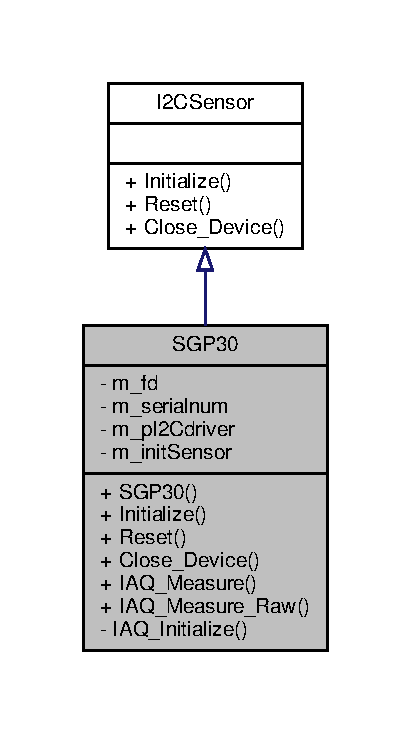
\includegraphics[width=197pt]{classSGP30__inherit__graph}
\end{center}
\end{figure}


Collaboration diagram for S\+G\+P30\+:\nopagebreak
\begin{figure}[H]
\begin{center}
\leavevmode
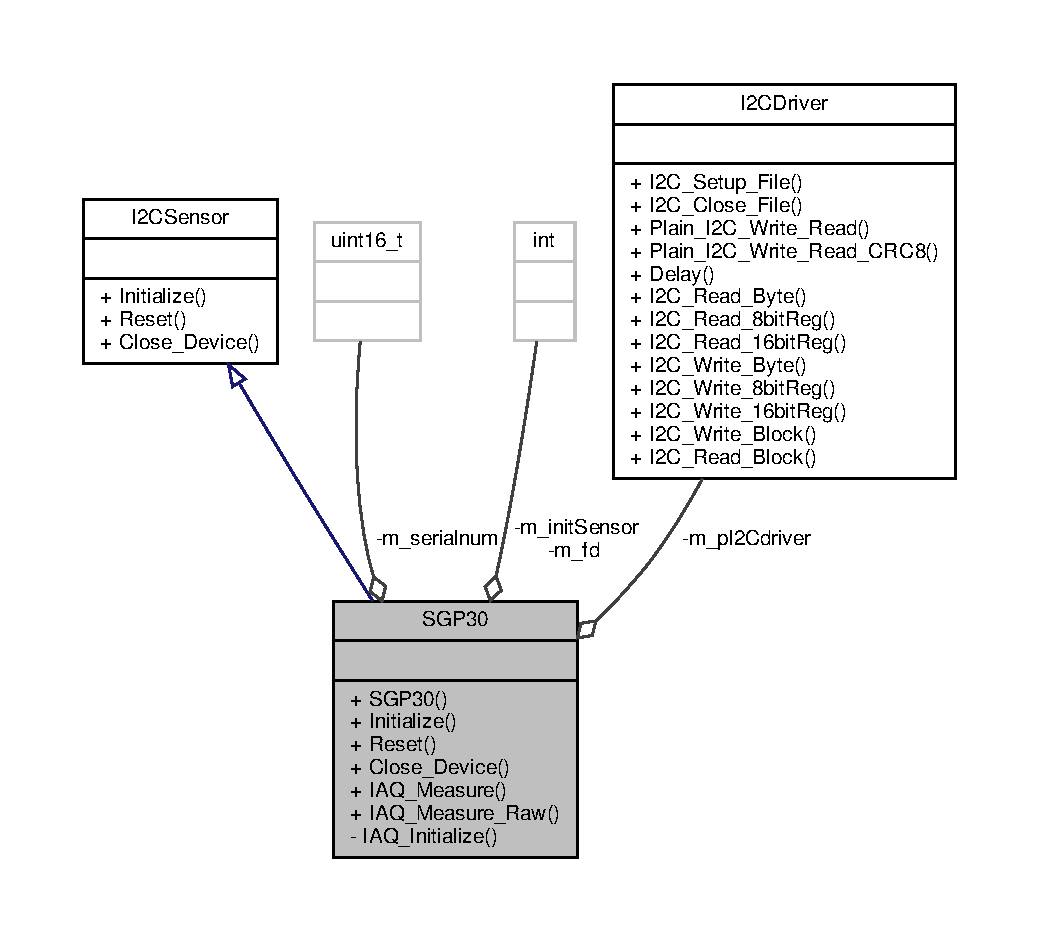
\includegraphics[width=350pt]{classSGP30__coll__graph}
\end{center}
\end{figure}
\subsection*{Public Member Functions}
\begin{DoxyCompactItemize}
\item 
\hyperlink{classSGP30_a995b5a2cf525479cbd930b54fb7d8f80}{S\+G\+P30} (void)
\item 
int \hyperlink{classSGP30_ad34fe8539ef007f55a0b3140889fdd6f}{Initialize} (\hyperlink{classI2CDriver}{I2\+C\+Driver} \&i2c) override
\item 
int \hyperlink{classSGP30_a4934ef3a64eb0782a6d956c6526e4186}{Reset} (void) override
\item 
int \hyperlink{classSGP30_a3feaf2623eb853169d14687e7ad1db24}{Close\+\_\+\+Device} (void) override
\item 
int \hyperlink{classSGP30_ac43bc058d733c27c6356ece89730232c}{I\+A\+Q\+\_\+\+Measure} (uint16\+\_\+t \&tvoc, uint16\+\_\+t \&e\+C\+O2)
\item 
int \hyperlink{classSGP30_aba7c9499ebc5a8aea6d3a5aaf23585ee}{I\+A\+Q\+\_\+\+Measure\+\_\+\+Raw} (uint16\+\_\+t \&raw\+Ethanol, uint16\+\_\+t \&raw\+H2)
\end{DoxyCompactItemize}
\subsection*{Private Types}
\begin{DoxyCompactItemize}
\item 
enum \{ \hyperlink{classSGP30_a5b752e81e00059c22c039ab0fa2021d0a509dbee04dff24f01fb2c7892703a3bd}{I2\+C\+\_\+\+A\+D\+D\+R\+E\+SS} = 0x58
 \}
\item 
enum \{ \hyperlink{classSGP30_a2729a6a324c09b992fbfc46fc4bfed66ae33bc9477a75eb531e3868a02ef79c78}{S\+G\+P30\+\_\+\+F\+E\+A\+T\+U\+R\+E\+S\+ET} = 0x0020
 \}
\item 
enum \{ \hyperlink{classSGP30_aacd1f082dc76bc6251edf06f0b3832c0ace04a9903c43bc54b35a579e0c661e13}{S\+G\+P30\+\_\+\+G\+E\+T\+\_\+\+S\+E\+R\+I\+A\+L\+\_\+\+ID} = 0x3682
 \}
\item 
enum \{ \hyperlink{classSGP30_aca7fa4ab06bdae25a5fb142ec20f58d3a9d732bc016196d5decb7e1dd2b1e2dd7}{S\+G\+P30\+\_\+\+G\+E\+T\+\_\+\+F\+E\+A\+T\+U\+R\+E\+S\+E\+T\+\_\+\+V\+E\+R\+S\+I\+ON} = 0x202F
 \}
\item 
enum \{ \hyperlink{classSGP30_a9fab3e307da43db87a836b096151a31ca68ef1f21f1267a8b1109796eea0e19fe}{S\+G\+P30\+\_\+\+I\+N\+I\+T\+\_\+\+A\+I\+R\+\_\+\+Q\+U\+A\+L\+I\+TY} = 0x2003
 \}
\item 
enum \{ \hyperlink{classSGP30_a7dc6849851676f2dbd1e118ff782d830a1d8427617ada8d841010c43f382bccfa}{S\+G\+P30\+\_\+\+M\+E\+A\+S\+U\+R\+E\+\_\+\+A\+I\+R\+\_\+\+Q\+U\+A\+L\+I\+TY} = 0x2008
 \}
\item 
enum \{ \hyperlink{classSGP30_a6265830ddaa1c5e55a1efe326326e57ea5df373d3deebce36ee7a1c745c9c735a}{S\+G\+P30\+\_\+\+G\+E\+T\+\_\+\+I\+A\+Q\+\_\+\+B\+A\+S\+E\+L\+I\+NE} = 0x2015
 \}
\item 
enum \{ \hyperlink{classSGP30_adb75f486c71b86401a9e61cf6d37449ba21711e444f927177674d89c44702904a}{S\+G\+P30\+\_\+\+S\+E\+T\+\_\+\+I\+A\+Q\+\_\+\+B\+A\+S\+E\+L\+I\+NE} = 0x201e
 \}
\item 
enum \{ \hyperlink{classSGP30_a4f249632f5e33f139cd7377c728cba1da8ad78d173fbf29a175db80bf59d8a361}{S\+G\+P30\+\_\+\+S\+E\+T\+\_\+\+A\+B\+S\+O\+L\+U\+T\+E\+\_\+\+H\+U\+M\+I\+D\+I\+TY} = 0x2061
 \}
\item 
enum \{ \hyperlink{classSGP30_af209e8391e943c53e3c6aa3479e4a8f9adaacf9a8f14c2f6903cdb635b3e8a1fd}{S\+G\+P30\+\_\+\+M\+E\+A\+S\+U\+R\+E\+\_\+\+T\+E\+ST} = 0x2032
 \}
\item 
enum \{ \hyperlink{classSGP30_a1d3a484196d7d31bf7d4210b410bb760a375ad7f464e6a21241bd655100a5ce94}{S\+G\+P30\+\_\+\+G\+E\+T\+\_\+\+F\+E\+A\+T\+U\+R\+E\+\_\+\+S\+ET} = 0x202f
 \}
\item 
enum \{ \hyperlink{classSGP30_ae79520d1a6d2d0b51a33f66bda330426a4b9de0c35084e50e2314402541630294}{S\+G\+P30\+\_\+\+M\+E\+A\+S\+U\+R\+E\+\_\+\+R\+AW} = 0x2050
 \}
\item 
enum \{ \hyperlink{classSGP30_aa3eee88b9594f8df87e651374c4a1016ac75ca98ed28bb4b660cde006d6ea03ed}{S\+G\+P30\+\_\+\+G\+E\+T\+\_\+\+T\+V\+O\+C\+\_\+\+I\+N\+C\+E\+P\+T\+I\+V\+E\+\_\+\+B\+A\+S\+E\+L\+I\+NE} = 0x20b3
 \}
\item 
enum \{ \hyperlink{classSGP30_a4a464453ec9603419c3d49ad5c3fd21ca2c77db1c8c9a871d505a7a54f13fa05f}{S\+G\+P30\+\_\+\+S\+E\+T\+\_\+\+T\+V\+O\+C\+\_\+\+B\+A\+S\+E\+L\+I\+NE} = 0x2077
 \}
\item 
enum \{ \hyperlink{classSGP30_a48c35303e4f88d4b9bed717184795c2eae7362fc1d71c48cca9c68611d5348007}{S\+G\+P30\+\_\+\+S\+O\+F\+T\+\_\+\+R\+E\+S\+ET} = 0x0006
 \}
\end{DoxyCompactItemize}
\subsection*{Private Member Functions}
\begin{DoxyCompactItemize}
\item 
int \hyperlink{classSGP30_a4419a25b8e25a133c3cfc876b3443669}{I\+A\+Q\+\_\+\+Initialize} (void)
\end{DoxyCompactItemize}
\subsection*{Private Attributes}
\begin{DoxyCompactItemize}
\item 
int \hyperlink{classSGP30_a751dee30db306b3f2ff17540adb7dfc9}{m\+\_\+fd}
\item 
uint16\+\_\+t \hyperlink{classSGP30_a6da04f39b302756d806d36ff3aa93293}{m\+\_\+serialnum} \mbox{[}3\mbox{]}
\item 
\hyperlink{classI2CDriver}{I2\+C\+Driver} $\ast$ \hyperlink{classSGP30_a3be2d504b90a81a66af2bcd4fc96673b}{m\+\_\+p\+I2\+Cdriver} = nullptr
\item 
int \hyperlink{classSGP30_a11b0db4fcffa5e8da8982a48ae0b1456}{m\+\_\+init\+Sensor}
\end{DoxyCompactItemize}


\subsection{Detailed Description}
\hyperlink{classSGP30}{S\+G\+P30} class. 

\begin{DoxyAuthor}{Author}
Kamil Rog
\end{DoxyAuthor}
This is class is responsilbe for the \hyperlink{classSGP30}{S\+G\+P30} gas sensor.

P\+R\+O\+T\+O\+C\+OL -\/ I2C

I2C 

\subsection{Member Enumeration Documentation}
\mbox{\Hypertarget{classSGP30_a5b752e81e00059c22c039ab0fa2021d0}\label{classSGP30_a5b752e81e00059c22c039ab0fa2021d0}} 
\subsubsection{\texorpdfstring{anonymous enum}{anonymous enum}}
{\footnotesize\ttfamily anonymous enum\hspace{0.3cm}{\ttfamily [private]}}

\begin{DoxyEnumFields}{Enumerator}
\raisebox{\heightof{T}}[0pt][0pt]{\index{I2\+C\+\_\+\+A\+D\+D\+R\+E\+SS@{I2\+C\+\_\+\+A\+D\+D\+R\+E\+SS}!S\+G\+P30@{S\+G\+P30}}\index{S\+G\+P30@{S\+G\+P30}!I2\+C\+\_\+\+A\+D\+D\+R\+E\+SS@{I2\+C\+\_\+\+A\+D\+D\+R\+E\+SS}}}\mbox{\Hypertarget{classSGP30_a5b752e81e00059c22c039ab0fa2021d0a509dbee04dff24f01fb2c7892703a3bd}\label{classSGP30_a5b752e81e00059c22c039ab0fa2021d0a509dbee04dff24f01fb2c7892703a3bd}} 
I2\+C\+\_\+\+A\+D\+D\+R\+E\+SS&\\
\hline

\end{DoxyEnumFields}
\mbox{\Hypertarget{classSGP30_a2729a6a324c09b992fbfc46fc4bfed66}\label{classSGP30_a2729a6a324c09b992fbfc46fc4bfed66}} 
\subsubsection{\texorpdfstring{anonymous enum}{anonymous enum}}
{\footnotesize\ttfamily anonymous enum\hspace{0.3cm}{\ttfamily [private]}}

\begin{DoxyEnumFields}{Enumerator}
\raisebox{\heightof{T}}[0pt][0pt]{\index{S\+G\+P30\+\_\+\+F\+E\+A\+T\+U\+R\+E\+S\+ET@{S\+G\+P30\+\_\+\+F\+E\+A\+T\+U\+R\+E\+S\+ET}!S\+G\+P30@{S\+G\+P30}}\index{S\+G\+P30@{S\+G\+P30}!S\+G\+P30\+\_\+\+F\+E\+A\+T\+U\+R\+E\+S\+ET@{S\+G\+P30\+\_\+\+F\+E\+A\+T\+U\+R\+E\+S\+ET}}}\mbox{\Hypertarget{classSGP30_a2729a6a324c09b992fbfc46fc4bfed66ae33bc9477a75eb531e3868a02ef79c78}\label{classSGP30_a2729a6a324c09b992fbfc46fc4bfed66ae33bc9477a75eb531e3868a02ef79c78}} 
S\+G\+P30\+\_\+\+F\+E\+A\+T\+U\+R\+E\+S\+ET&\\
\hline

\end{DoxyEnumFields}
\mbox{\Hypertarget{classSGP30_a1d3a484196d7d31bf7d4210b410bb760}\label{classSGP30_a1d3a484196d7d31bf7d4210b410bb760}} 
\subsubsection{\texorpdfstring{anonymous enum}{anonymous enum}}
{\footnotesize\ttfamily anonymous enum\hspace{0.3cm}{\ttfamily [private]}}

\begin{DoxyEnumFields}{Enumerator}
\raisebox{\heightof{T}}[0pt][0pt]{\index{S\+G\+P30\+\_\+\+G\+E\+T\+\_\+\+F\+E\+A\+T\+U\+R\+E\+\_\+\+S\+ET@{S\+G\+P30\+\_\+\+G\+E\+T\+\_\+\+F\+E\+A\+T\+U\+R\+E\+\_\+\+S\+ET}!S\+G\+P30@{S\+G\+P30}}\index{S\+G\+P30@{S\+G\+P30}!S\+G\+P30\+\_\+\+G\+E\+T\+\_\+\+F\+E\+A\+T\+U\+R\+E\+\_\+\+S\+ET@{S\+G\+P30\+\_\+\+G\+E\+T\+\_\+\+F\+E\+A\+T\+U\+R\+E\+\_\+\+S\+ET}}}\mbox{\Hypertarget{classSGP30_a1d3a484196d7d31bf7d4210b410bb760a375ad7f464e6a21241bd655100a5ce94}\label{classSGP30_a1d3a484196d7d31bf7d4210b410bb760a375ad7f464e6a21241bd655100a5ce94}} 
S\+G\+P30\+\_\+\+G\+E\+T\+\_\+\+F\+E\+A\+T\+U\+R\+E\+\_\+\+S\+ET&\\
\hline

\end{DoxyEnumFields}
\mbox{\Hypertarget{classSGP30_ae79520d1a6d2d0b51a33f66bda330426}\label{classSGP30_ae79520d1a6d2d0b51a33f66bda330426}} 
\subsubsection{\texorpdfstring{anonymous enum}{anonymous enum}}
{\footnotesize\ttfamily anonymous enum\hspace{0.3cm}{\ttfamily [private]}}

\begin{DoxyEnumFields}{Enumerator}
\raisebox{\heightof{T}}[0pt][0pt]{\index{S\+G\+P30\+\_\+\+M\+E\+A\+S\+U\+R\+E\+\_\+\+R\+AW@{S\+G\+P30\+\_\+\+M\+E\+A\+S\+U\+R\+E\+\_\+\+R\+AW}!S\+G\+P30@{S\+G\+P30}}\index{S\+G\+P30@{S\+G\+P30}!S\+G\+P30\+\_\+\+M\+E\+A\+S\+U\+R\+E\+\_\+\+R\+AW@{S\+G\+P30\+\_\+\+M\+E\+A\+S\+U\+R\+E\+\_\+\+R\+AW}}}\mbox{\Hypertarget{classSGP30_ae79520d1a6d2d0b51a33f66bda330426a4b9de0c35084e50e2314402541630294}\label{classSGP30_ae79520d1a6d2d0b51a33f66bda330426a4b9de0c35084e50e2314402541630294}} 
S\+G\+P30\+\_\+\+M\+E\+A\+S\+U\+R\+E\+\_\+\+R\+AW&\\
\hline

\end{DoxyEnumFields}
\mbox{\Hypertarget{classSGP30_aa3eee88b9594f8df87e651374c4a1016}\label{classSGP30_aa3eee88b9594f8df87e651374c4a1016}} 
\subsubsection{\texorpdfstring{anonymous enum}{anonymous enum}}
{\footnotesize\ttfamily anonymous enum\hspace{0.3cm}{\ttfamily [private]}}

\begin{DoxyEnumFields}{Enumerator}
\raisebox{\heightof{T}}[0pt][0pt]{\index{S\+G\+P30\+\_\+\+G\+E\+T\+\_\+\+T\+V\+O\+C\+\_\+\+I\+N\+C\+E\+P\+T\+I\+V\+E\+\_\+\+B\+A\+S\+E\+L\+I\+NE@{S\+G\+P30\+\_\+\+G\+E\+T\+\_\+\+T\+V\+O\+C\+\_\+\+I\+N\+C\+E\+P\+T\+I\+V\+E\+\_\+\+B\+A\+S\+E\+L\+I\+NE}!S\+G\+P30@{S\+G\+P30}}\index{S\+G\+P30@{S\+G\+P30}!S\+G\+P30\+\_\+\+G\+E\+T\+\_\+\+T\+V\+O\+C\+\_\+\+I\+N\+C\+E\+P\+T\+I\+V\+E\+\_\+\+B\+A\+S\+E\+L\+I\+NE@{S\+G\+P30\+\_\+\+G\+E\+T\+\_\+\+T\+V\+O\+C\+\_\+\+I\+N\+C\+E\+P\+T\+I\+V\+E\+\_\+\+B\+A\+S\+E\+L\+I\+NE}}}\mbox{\Hypertarget{classSGP30_aa3eee88b9594f8df87e651374c4a1016ac75ca98ed28bb4b660cde006d6ea03ed}\label{classSGP30_aa3eee88b9594f8df87e651374c4a1016ac75ca98ed28bb4b660cde006d6ea03ed}} 
S\+G\+P30\+\_\+\+G\+E\+T\+\_\+\+T\+V\+O\+C\+\_\+\+I\+N\+C\+E\+P\+T\+I\+V\+E\+\_\+\+B\+A\+S\+E\+L\+I\+NE&\\
\hline

\end{DoxyEnumFields}
\mbox{\Hypertarget{classSGP30_a4a464453ec9603419c3d49ad5c3fd21c}\label{classSGP30_a4a464453ec9603419c3d49ad5c3fd21c}} 
\subsubsection{\texorpdfstring{anonymous enum}{anonymous enum}}
{\footnotesize\ttfamily anonymous enum\hspace{0.3cm}{\ttfamily [private]}}

\begin{DoxyEnumFields}{Enumerator}
\raisebox{\heightof{T}}[0pt][0pt]{\index{S\+G\+P30\+\_\+\+S\+E\+T\+\_\+\+T\+V\+O\+C\+\_\+\+B\+A\+S\+E\+L\+I\+NE@{S\+G\+P30\+\_\+\+S\+E\+T\+\_\+\+T\+V\+O\+C\+\_\+\+B\+A\+S\+E\+L\+I\+NE}!S\+G\+P30@{S\+G\+P30}}\index{S\+G\+P30@{S\+G\+P30}!S\+G\+P30\+\_\+\+S\+E\+T\+\_\+\+T\+V\+O\+C\+\_\+\+B\+A\+S\+E\+L\+I\+NE@{S\+G\+P30\+\_\+\+S\+E\+T\+\_\+\+T\+V\+O\+C\+\_\+\+B\+A\+S\+E\+L\+I\+NE}}}\mbox{\Hypertarget{classSGP30_a4a464453ec9603419c3d49ad5c3fd21ca2c77db1c8c9a871d505a7a54f13fa05f}\label{classSGP30_a4a464453ec9603419c3d49ad5c3fd21ca2c77db1c8c9a871d505a7a54f13fa05f}} 
S\+G\+P30\+\_\+\+S\+E\+T\+\_\+\+T\+V\+O\+C\+\_\+\+B\+A\+S\+E\+L\+I\+NE&\\
\hline

\end{DoxyEnumFields}
\mbox{\Hypertarget{classSGP30_a48c35303e4f88d4b9bed717184795c2e}\label{classSGP30_a48c35303e4f88d4b9bed717184795c2e}} 
\subsubsection{\texorpdfstring{anonymous enum}{anonymous enum}}
{\footnotesize\ttfamily anonymous enum\hspace{0.3cm}{\ttfamily [private]}}

\begin{DoxyEnumFields}{Enumerator}
\raisebox{\heightof{T}}[0pt][0pt]{\index{S\+G\+P30\+\_\+\+S\+O\+F\+T\+\_\+\+R\+E\+S\+ET@{S\+G\+P30\+\_\+\+S\+O\+F\+T\+\_\+\+R\+E\+S\+ET}!S\+G\+P30@{S\+G\+P30}}\index{S\+G\+P30@{S\+G\+P30}!S\+G\+P30\+\_\+\+S\+O\+F\+T\+\_\+\+R\+E\+S\+ET@{S\+G\+P30\+\_\+\+S\+O\+F\+T\+\_\+\+R\+E\+S\+ET}}}\mbox{\Hypertarget{classSGP30_a48c35303e4f88d4b9bed717184795c2eae7362fc1d71c48cca9c68611d5348007}\label{classSGP30_a48c35303e4f88d4b9bed717184795c2eae7362fc1d71c48cca9c68611d5348007}} 
S\+G\+P30\+\_\+\+S\+O\+F\+T\+\_\+\+R\+E\+S\+ET&\\
\hline

\end{DoxyEnumFields}
\mbox{\Hypertarget{classSGP30_aacd1f082dc76bc6251edf06f0b3832c0}\label{classSGP30_aacd1f082dc76bc6251edf06f0b3832c0}} 
\subsubsection{\texorpdfstring{anonymous enum}{anonymous enum}}
{\footnotesize\ttfamily anonymous enum\hspace{0.3cm}{\ttfamily [private]}}

\begin{DoxyEnumFields}{Enumerator}
\raisebox{\heightof{T}}[0pt][0pt]{\index{S\+G\+P30\+\_\+\+G\+E\+T\+\_\+\+S\+E\+R\+I\+A\+L\+\_\+\+ID@{S\+G\+P30\+\_\+\+G\+E\+T\+\_\+\+S\+E\+R\+I\+A\+L\+\_\+\+ID}!S\+G\+P30@{S\+G\+P30}}\index{S\+G\+P30@{S\+G\+P30}!S\+G\+P30\+\_\+\+G\+E\+T\+\_\+\+S\+E\+R\+I\+A\+L\+\_\+\+ID@{S\+G\+P30\+\_\+\+G\+E\+T\+\_\+\+S\+E\+R\+I\+A\+L\+\_\+\+ID}}}\mbox{\Hypertarget{classSGP30_aacd1f082dc76bc6251edf06f0b3832c0ace04a9903c43bc54b35a579e0c661e13}\label{classSGP30_aacd1f082dc76bc6251edf06f0b3832c0ace04a9903c43bc54b35a579e0c661e13}} 
S\+G\+P30\+\_\+\+G\+E\+T\+\_\+\+S\+E\+R\+I\+A\+L\+\_\+\+ID&\\
\hline

\end{DoxyEnumFields}
\mbox{\Hypertarget{classSGP30_aca7fa4ab06bdae25a5fb142ec20f58d3}\label{classSGP30_aca7fa4ab06bdae25a5fb142ec20f58d3}} 
\subsubsection{\texorpdfstring{anonymous enum}{anonymous enum}}
{\footnotesize\ttfamily anonymous enum\hspace{0.3cm}{\ttfamily [private]}}

\begin{DoxyEnumFields}{Enumerator}
\raisebox{\heightof{T}}[0pt][0pt]{\index{S\+G\+P30\+\_\+\+G\+E\+T\+\_\+\+F\+E\+A\+T\+U\+R\+E\+S\+E\+T\+\_\+\+V\+E\+R\+S\+I\+ON@{S\+G\+P30\+\_\+\+G\+E\+T\+\_\+\+F\+E\+A\+T\+U\+R\+E\+S\+E\+T\+\_\+\+V\+E\+R\+S\+I\+ON}!S\+G\+P30@{S\+G\+P30}}\index{S\+G\+P30@{S\+G\+P30}!S\+G\+P30\+\_\+\+G\+E\+T\+\_\+\+F\+E\+A\+T\+U\+R\+E\+S\+E\+T\+\_\+\+V\+E\+R\+S\+I\+ON@{S\+G\+P30\+\_\+\+G\+E\+T\+\_\+\+F\+E\+A\+T\+U\+R\+E\+S\+E\+T\+\_\+\+V\+E\+R\+S\+I\+ON}}}\mbox{\Hypertarget{classSGP30_aca7fa4ab06bdae25a5fb142ec20f58d3a9d732bc016196d5decb7e1dd2b1e2dd7}\label{classSGP30_aca7fa4ab06bdae25a5fb142ec20f58d3a9d732bc016196d5decb7e1dd2b1e2dd7}} 
S\+G\+P30\+\_\+\+G\+E\+T\+\_\+\+F\+E\+A\+T\+U\+R\+E\+S\+E\+T\+\_\+\+V\+E\+R\+S\+I\+ON&\\
\hline

\end{DoxyEnumFields}
\mbox{\Hypertarget{classSGP30_a9fab3e307da43db87a836b096151a31c}\label{classSGP30_a9fab3e307da43db87a836b096151a31c}} 
\subsubsection{\texorpdfstring{anonymous enum}{anonymous enum}}
{\footnotesize\ttfamily anonymous enum\hspace{0.3cm}{\ttfamily [private]}}

\begin{DoxyEnumFields}{Enumerator}
\raisebox{\heightof{T}}[0pt][0pt]{\index{S\+G\+P30\+\_\+\+I\+N\+I\+T\+\_\+\+A\+I\+R\+\_\+\+Q\+U\+A\+L\+I\+TY@{S\+G\+P30\+\_\+\+I\+N\+I\+T\+\_\+\+A\+I\+R\+\_\+\+Q\+U\+A\+L\+I\+TY}!S\+G\+P30@{S\+G\+P30}}\index{S\+G\+P30@{S\+G\+P30}!S\+G\+P30\+\_\+\+I\+N\+I\+T\+\_\+\+A\+I\+R\+\_\+\+Q\+U\+A\+L\+I\+TY@{S\+G\+P30\+\_\+\+I\+N\+I\+T\+\_\+\+A\+I\+R\+\_\+\+Q\+U\+A\+L\+I\+TY}}}\mbox{\Hypertarget{classSGP30_a9fab3e307da43db87a836b096151a31ca68ef1f21f1267a8b1109796eea0e19fe}\label{classSGP30_a9fab3e307da43db87a836b096151a31ca68ef1f21f1267a8b1109796eea0e19fe}} 
S\+G\+P30\+\_\+\+I\+N\+I\+T\+\_\+\+A\+I\+R\+\_\+\+Q\+U\+A\+L\+I\+TY&\\
\hline

\end{DoxyEnumFields}
\mbox{\Hypertarget{classSGP30_a7dc6849851676f2dbd1e118ff782d830}\label{classSGP30_a7dc6849851676f2dbd1e118ff782d830}} 
\subsubsection{\texorpdfstring{anonymous enum}{anonymous enum}}
{\footnotesize\ttfamily anonymous enum\hspace{0.3cm}{\ttfamily [private]}}

\begin{DoxyEnumFields}{Enumerator}
\raisebox{\heightof{T}}[0pt][0pt]{\index{S\+G\+P30\+\_\+\+M\+E\+A\+S\+U\+R\+E\+\_\+\+A\+I\+R\+\_\+\+Q\+U\+A\+L\+I\+TY@{S\+G\+P30\+\_\+\+M\+E\+A\+S\+U\+R\+E\+\_\+\+A\+I\+R\+\_\+\+Q\+U\+A\+L\+I\+TY}!S\+G\+P30@{S\+G\+P30}}\index{S\+G\+P30@{S\+G\+P30}!S\+G\+P30\+\_\+\+M\+E\+A\+S\+U\+R\+E\+\_\+\+A\+I\+R\+\_\+\+Q\+U\+A\+L\+I\+TY@{S\+G\+P30\+\_\+\+M\+E\+A\+S\+U\+R\+E\+\_\+\+A\+I\+R\+\_\+\+Q\+U\+A\+L\+I\+TY}}}\mbox{\Hypertarget{classSGP30_a7dc6849851676f2dbd1e118ff782d830a1d8427617ada8d841010c43f382bccfa}\label{classSGP30_a7dc6849851676f2dbd1e118ff782d830a1d8427617ada8d841010c43f382bccfa}} 
S\+G\+P30\+\_\+\+M\+E\+A\+S\+U\+R\+E\+\_\+\+A\+I\+R\+\_\+\+Q\+U\+A\+L\+I\+TY&\\
\hline

\end{DoxyEnumFields}
\mbox{\Hypertarget{classSGP30_a6265830ddaa1c5e55a1efe326326e57e}\label{classSGP30_a6265830ddaa1c5e55a1efe326326e57e}} 
\subsubsection{\texorpdfstring{anonymous enum}{anonymous enum}}
{\footnotesize\ttfamily anonymous enum\hspace{0.3cm}{\ttfamily [private]}}

\begin{DoxyEnumFields}{Enumerator}
\raisebox{\heightof{T}}[0pt][0pt]{\index{S\+G\+P30\+\_\+\+G\+E\+T\+\_\+\+I\+A\+Q\+\_\+\+B\+A\+S\+E\+L\+I\+NE@{S\+G\+P30\+\_\+\+G\+E\+T\+\_\+\+I\+A\+Q\+\_\+\+B\+A\+S\+E\+L\+I\+NE}!S\+G\+P30@{S\+G\+P30}}\index{S\+G\+P30@{S\+G\+P30}!S\+G\+P30\+\_\+\+G\+E\+T\+\_\+\+I\+A\+Q\+\_\+\+B\+A\+S\+E\+L\+I\+NE@{S\+G\+P30\+\_\+\+G\+E\+T\+\_\+\+I\+A\+Q\+\_\+\+B\+A\+S\+E\+L\+I\+NE}}}\mbox{\Hypertarget{classSGP30_a6265830ddaa1c5e55a1efe326326e57ea5df373d3deebce36ee7a1c745c9c735a}\label{classSGP30_a6265830ddaa1c5e55a1efe326326e57ea5df373d3deebce36ee7a1c745c9c735a}} 
S\+G\+P30\+\_\+\+G\+E\+T\+\_\+\+I\+A\+Q\+\_\+\+B\+A\+S\+E\+L\+I\+NE&\\
\hline

\end{DoxyEnumFields}
\mbox{\Hypertarget{classSGP30_adb75f486c71b86401a9e61cf6d37449b}\label{classSGP30_adb75f486c71b86401a9e61cf6d37449b}} 
\subsubsection{\texorpdfstring{anonymous enum}{anonymous enum}}
{\footnotesize\ttfamily anonymous enum\hspace{0.3cm}{\ttfamily [private]}}

\begin{DoxyEnumFields}{Enumerator}
\raisebox{\heightof{T}}[0pt][0pt]{\index{S\+G\+P30\+\_\+\+S\+E\+T\+\_\+\+I\+A\+Q\+\_\+\+B\+A\+S\+E\+L\+I\+NE@{S\+G\+P30\+\_\+\+S\+E\+T\+\_\+\+I\+A\+Q\+\_\+\+B\+A\+S\+E\+L\+I\+NE}!S\+G\+P30@{S\+G\+P30}}\index{S\+G\+P30@{S\+G\+P30}!S\+G\+P30\+\_\+\+S\+E\+T\+\_\+\+I\+A\+Q\+\_\+\+B\+A\+S\+E\+L\+I\+NE@{S\+G\+P30\+\_\+\+S\+E\+T\+\_\+\+I\+A\+Q\+\_\+\+B\+A\+S\+E\+L\+I\+NE}}}\mbox{\Hypertarget{classSGP30_adb75f486c71b86401a9e61cf6d37449ba21711e444f927177674d89c44702904a}\label{classSGP30_adb75f486c71b86401a9e61cf6d37449ba21711e444f927177674d89c44702904a}} 
S\+G\+P30\+\_\+\+S\+E\+T\+\_\+\+I\+A\+Q\+\_\+\+B\+A\+S\+E\+L\+I\+NE&\\
\hline

\end{DoxyEnumFields}
\mbox{\Hypertarget{classSGP30_a4f249632f5e33f139cd7377c728cba1d}\label{classSGP30_a4f249632f5e33f139cd7377c728cba1d}} 
\subsubsection{\texorpdfstring{anonymous enum}{anonymous enum}}
{\footnotesize\ttfamily anonymous enum\hspace{0.3cm}{\ttfamily [private]}}

\begin{DoxyEnumFields}{Enumerator}
\raisebox{\heightof{T}}[0pt][0pt]{\index{S\+G\+P30\+\_\+\+S\+E\+T\+\_\+\+A\+B\+S\+O\+L\+U\+T\+E\+\_\+\+H\+U\+M\+I\+D\+I\+TY@{S\+G\+P30\+\_\+\+S\+E\+T\+\_\+\+A\+B\+S\+O\+L\+U\+T\+E\+\_\+\+H\+U\+M\+I\+D\+I\+TY}!S\+G\+P30@{S\+G\+P30}}\index{S\+G\+P30@{S\+G\+P30}!S\+G\+P30\+\_\+\+S\+E\+T\+\_\+\+A\+B\+S\+O\+L\+U\+T\+E\+\_\+\+H\+U\+M\+I\+D\+I\+TY@{S\+G\+P30\+\_\+\+S\+E\+T\+\_\+\+A\+B\+S\+O\+L\+U\+T\+E\+\_\+\+H\+U\+M\+I\+D\+I\+TY}}}\mbox{\Hypertarget{classSGP30_a4f249632f5e33f139cd7377c728cba1da8ad78d173fbf29a175db80bf59d8a361}\label{classSGP30_a4f249632f5e33f139cd7377c728cba1da8ad78d173fbf29a175db80bf59d8a361}} 
S\+G\+P30\+\_\+\+S\+E\+T\+\_\+\+A\+B\+S\+O\+L\+U\+T\+E\+\_\+\+H\+U\+M\+I\+D\+I\+TY&\\
\hline

\end{DoxyEnumFields}
\mbox{\Hypertarget{classSGP30_af209e8391e943c53e3c6aa3479e4a8f9}\label{classSGP30_af209e8391e943c53e3c6aa3479e4a8f9}} 
\subsubsection{\texorpdfstring{anonymous enum}{anonymous enum}}
{\footnotesize\ttfamily anonymous enum\hspace{0.3cm}{\ttfamily [private]}}

\begin{DoxyEnumFields}{Enumerator}
\raisebox{\heightof{T}}[0pt][0pt]{\index{S\+G\+P30\+\_\+\+M\+E\+A\+S\+U\+R\+E\+\_\+\+T\+E\+ST@{S\+G\+P30\+\_\+\+M\+E\+A\+S\+U\+R\+E\+\_\+\+T\+E\+ST}!S\+G\+P30@{S\+G\+P30}}\index{S\+G\+P30@{S\+G\+P30}!S\+G\+P30\+\_\+\+M\+E\+A\+S\+U\+R\+E\+\_\+\+T\+E\+ST@{S\+G\+P30\+\_\+\+M\+E\+A\+S\+U\+R\+E\+\_\+\+T\+E\+ST}}}\mbox{\Hypertarget{classSGP30_af209e8391e943c53e3c6aa3479e4a8f9adaacf9a8f14c2f6903cdb635b3e8a1fd}\label{classSGP30_af209e8391e943c53e3c6aa3479e4a8f9adaacf9a8f14c2f6903cdb635b3e8a1fd}} 
S\+G\+P30\+\_\+\+M\+E\+A\+S\+U\+R\+E\+\_\+\+T\+E\+ST&\\
\hline

\end{DoxyEnumFields}


\subsection{Constructor \& Destructor Documentation}
\mbox{\Hypertarget{classSGP30_a995b5a2cf525479cbd930b54fb7d8f80}\label{classSGP30_a995b5a2cf525479cbd930b54fb7d8f80}} 
\index{S\+G\+P30@{S\+G\+P30}!S\+G\+P30@{S\+G\+P30}}
\index{S\+G\+P30@{S\+G\+P30}!S\+G\+P30@{S\+G\+P30}}
\subsubsection{\texorpdfstring{S\+G\+P30()}{SGP30()}}
{\footnotesize\ttfamily S\+G\+P30\+::\+S\+G\+P30 (\begin{DoxyParamCaption}\item[{void}]{ }\end{DoxyParamCaption})\hspace{0.3cm}{\ttfamily [inline]}}



\subsection{Member Function Documentation}
\mbox{\Hypertarget{classSGP30_a3feaf2623eb853169d14687e7ad1db24}\label{classSGP30_a3feaf2623eb853169d14687e7ad1db24}} 
\index{S\+G\+P30@{S\+G\+P30}!Close\+\_\+\+Device@{Close\+\_\+\+Device}}
\index{Close\+\_\+\+Device@{Close\+\_\+\+Device}!S\+G\+P30@{S\+G\+P30}}
\subsubsection{\texorpdfstring{Close\+\_\+\+Device()}{Close\_Device()}}
{\footnotesize\ttfamily int S\+G\+P30\+::\+Close\+\_\+\+Device (\begin{DoxyParamCaption}\item[{void}]{ }\end{DoxyParamCaption})\hspace{0.3cm}{\ttfamily [override]}, {\ttfamily [virtual]}}

Closes device Firstly Resets the sensor and then closes file descriptor

\begin{DoxyReturn}{Returns}
Status of close operation 
\end{DoxyReturn}


Implements \hyperlink{classI2CSensor_acee1633439e97bae412441ac085fabba}{I2\+C\+Sensor}.

\mbox{\Hypertarget{classSGP30_a4419a25b8e25a133c3cfc876b3443669}\label{classSGP30_a4419a25b8e25a133c3cfc876b3443669}} 
\index{S\+G\+P30@{S\+G\+P30}!I\+A\+Q\+\_\+\+Initialize@{I\+A\+Q\+\_\+\+Initialize}}
\index{I\+A\+Q\+\_\+\+Initialize@{I\+A\+Q\+\_\+\+Initialize}!S\+G\+P30@{S\+G\+P30}}
\subsubsection{\texorpdfstring{I\+A\+Q\+\_\+\+Initialize()}{IAQ\_Initialize()}}
{\footnotesize\ttfamily int S\+G\+P30\+::\+I\+A\+Q\+\_\+\+Initialize (\begin{DoxyParamCaption}\item[{void}]{ }\end{DoxyParamCaption})\hspace{0.3cm}{\ttfamily [private]}}

Start I\+AQ algorithm. Must be called in initalization stage.

\begin{DoxyReturn}{Returns}
Zero on success else negative errno 
\end{DoxyReturn}
\mbox{\Hypertarget{classSGP30_ac43bc058d733c27c6356ece89730232c}\label{classSGP30_ac43bc058d733c27c6356ece89730232c}} 
\index{S\+G\+P30@{S\+G\+P30}!I\+A\+Q\+\_\+\+Measure@{I\+A\+Q\+\_\+\+Measure}}
\index{I\+A\+Q\+\_\+\+Measure@{I\+A\+Q\+\_\+\+Measure}!S\+G\+P30@{S\+G\+P30}}
\subsubsection{\texorpdfstring{I\+A\+Q\+\_\+\+Measure()}{IAQ\_Measure()}}
{\footnotesize\ttfamily int S\+G\+P30\+::\+I\+A\+Q\+\_\+\+Measure (\begin{DoxyParamCaption}\item[{uint16\+\_\+t \&}]{tvoc,  }\item[{uint16\+\_\+t \&}]{e\+C\+O2 }\end{DoxyParamCaption})}

Take a single e\+C\+O2 \& T\+V\+OC raw measurement


\begin{DoxyParams}{Parameters}
{\em tvoc} & Address of the tvoc variable to modify. \\
\hline
{\em e\+C\+O2} & Address of the eco2 variable to modify\\
\hline
\end{DoxyParams}
\begin{DoxyReturn}{Returns}
Zero on success else negative error number 
\end{DoxyReturn}
\mbox{\Hypertarget{classSGP30_aba7c9499ebc5a8aea6d3a5aaf23585ee}\label{classSGP30_aba7c9499ebc5a8aea6d3a5aaf23585ee}} 
\index{S\+G\+P30@{S\+G\+P30}!I\+A\+Q\+\_\+\+Measure\+\_\+\+Raw@{I\+A\+Q\+\_\+\+Measure\+\_\+\+Raw}}
\index{I\+A\+Q\+\_\+\+Measure\+\_\+\+Raw@{I\+A\+Q\+\_\+\+Measure\+\_\+\+Raw}!S\+G\+P30@{S\+G\+P30}}
\subsubsection{\texorpdfstring{I\+A\+Q\+\_\+\+Measure\+\_\+\+Raw()}{IAQ\_Measure\_Raw()}}
{\footnotesize\ttfamily int S\+G\+P30\+::\+I\+A\+Q\+\_\+\+Measure\+\_\+\+Raw (\begin{DoxyParamCaption}\item[{uint16\+\_\+t \&}]{raw\+Ethanol,  }\item[{uint16\+\_\+t \&}]{raw\+H2 }\end{DoxyParamCaption})}

Take a single H2 \& ethanol raw measurement.


\begin{DoxyParams}{Parameters}
{\em raw\+Ethanol} & Address of the raw\+Ethanol variable to modify. \\
\hline
{\em raw\+H2} & Address of the raw\+H2 variable to modify\\
\hline
\end{DoxyParams}
\begin{DoxyReturn}{Returns}
Zero on success else negative error number 
\end{DoxyReturn}
\mbox{\Hypertarget{classSGP30_ad34fe8539ef007f55a0b3140889fdd6f}\label{classSGP30_ad34fe8539ef007f55a0b3140889fdd6f}} 
\index{S\+G\+P30@{S\+G\+P30}!Initialize@{Initialize}}
\index{Initialize@{Initialize}!S\+G\+P30@{S\+G\+P30}}
\subsubsection{\texorpdfstring{Initialize()}{Initialize()}}
{\footnotesize\ttfamily int S\+G\+P30\+::\+Initialize (\begin{DoxyParamCaption}\item[{\hyperlink{classI2CDriver}{I2\+C\+Driver} \&}]{i2c }\end{DoxyParamCaption})\hspace{0.3cm}{\ttfamily [override]}, {\ttfamily [virtual]}}

Initialize \hyperlink{classSHT31D}{S\+H\+T31D} Open file descriptor

\begin{DoxyReturn}{Returns}
None 
\end{DoxyReturn}


Implements \hyperlink{classI2CSensor_a0fb4755ddff3fe2cf5a9651d9d1fe5cd}{I2\+C\+Sensor}.

\mbox{\Hypertarget{classSGP30_a4934ef3a64eb0782a6d956c6526e4186}\label{classSGP30_a4934ef3a64eb0782a6d956c6526e4186}} 
\index{S\+G\+P30@{S\+G\+P30}!Reset@{Reset}}
\index{Reset@{Reset}!S\+G\+P30@{S\+G\+P30}}
\subsubsection{\texorpdfstring{Reset()}{Reset()}}
{\footnotesize\ttfamily int S\+G\+P30\+::\+Reset (\begin{DoxyParamCaption}\item[{void}]{ }\end{DoxyParamCaption})\hspace{0.3cm}{\ttfamily [override]}, {\ttfamily [virtual]}}

Soft Reset \hyperlink{classSGP30}{S\+G\+P30}

\begin{DoxyReturn}{Returns}
Zero on success else negative error number 
\end{DoxyReturn}


Implements \hyperlink{classI2CSensor_a0622266d335944782d2bfa6352f01095}{I2\+C\+Sensor}.



\subsection{Member Data Documentation}
\mbox{\Hypertarget{classSGP30_a751dee30db306b3f2ff17540adb7dfc9}\label{classSGP30_a751dee30db306b3f2ff17540adb7dfc9}} 
\index{S\+G\+P30@{S\+G\+P30}!m\+\_\+fd@{m\+\_\+fd}}
\index{m\+\_\+fd@{m\+\_\+fd}!S\+G\+P30@{S\+G\+P30}}
\subsubsection{\texorpdfstring{m\+\_\+fd}{m\_fd}}
{\footnotesize\ttfamily int S\+G\+P30\+::m\+\_\+fd\hspace{0.3cm}{\ttfamily [private]}}

\mbox{\Hypertarget{classSGP30_a11b0db4fcffa5e8da8982a48ae0b1456}\label{classSGP30_a11b0db4fcffa5e8da8982a48ae0b1456}} 
\index{S\+G\+P30@{S\+G\+P30}!m\+\_\+init\+Sensor@{m\+\_\+init\+Sensor}}
\index{m\+\_\+init\+Sensor@{m\+\_\+init\+Sensor}!S\+G\+P30@{S\+G\+P30}}
\subsubsection{\texorpdfstring{m\+\_\+init\+Sensor}{m\_initSensor}}
{\footnotesize\ttfamily int S\+G\+P30\+::m\+\_\+init\+Sensor\hspace{0.3cm}{\ttfamily [private]}}

\mbox{\Hypertarget{classSGP30_a3be2d504b90a81a66af2bcd4fc96673b}\label{classSGP30_a3be2d504b90a81a66af2bcd4fc96673b}} 
\index{S\+G\+P30@{S\+G\+P30}!m\+\_\+p\+I2\+Cdriver@{m\+\_\+p\+I2\+Cdriver}}
\index{m\+\_\+p\+I2\+Cdriver@{m\+\_\+p\+I2\+Cdriver}!S\+G\+P30@{S\+G\+P30}}
\subsubsection{\texorpdfstring{m\+\_\+p\+I2\+Cdriver}{m\_pI2Cdriver}}
{\footnotesize\ttfamily \hyperlink{classI2CDriver}{I2\+C\+Driver}$\ast$ S\+G\+P30\+::m\+\_\+p\+I2\+Cdriver = nullptr\hspace{0.3cm}{\ttfamily [private]}}

\mbox{\Hypertarget{classSGP30_a6da04f39b302756d806d36ff3aa93293}\label{classSGP30_a6da04f39b302756d806d36ff3aa93293}} 
\index{S\+G\+P30@{S\+G\+P30}!m\+\_\+serialnum@{m\+\_\+serialnum}}
\index{m\+\_\+serialnum@{m\+\_\+serialnum}!S\+G\+P30@{S\+G\+P30}}
\subsubsection{\texorpdfstring{m\+\_\+serialnum}{m\_serialnum}}
{\footnotesize\ttfamily uint16\+\_\+t S\+G\+P30\+::m\+\_\+serialnum\mbox{[}3\mbox{]}\hspace{0.3cm}{\ttfamily [private]}}



The documentation for this class was generated from the following files\+:\begin{DoxyCompactItemize}
\item 
src/controller/peripherials/\hyperlink{SGP30_8h}{S\+G\+P30.\+h}\item 
src/controller/peripherials/\hyperlink{SGP30_8cpp}{S\+G\+P30.\+cpp}\end{DoxyCompactItemize}

\hypertarget{classSHT31D}{}\section{S\+H\+T31D Class Reference}
\label{classSHT31D}\index{S\+H\+T31D@{S\+H\+T31D}}


\hyperlink{classSHT31D}{S\+H\+T31D} class.  




{\ttfamily \#include $<$S\+H\+T31\+D.\+h$>$}



Inheritance diagram for S\+H\+T31D\+:\nopagebreak
\begin{figure}[H]
\begin{center}
\leavevmode
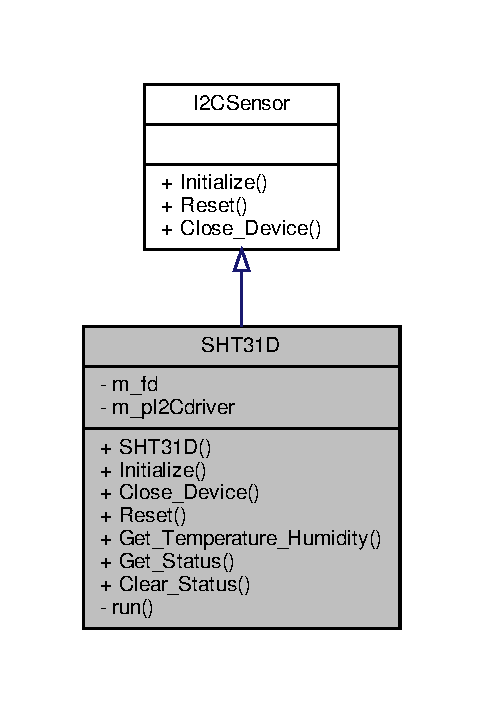
\includegraphics[width=232pt]{classSHT31D__inherit__graph}
\end{center}
\end{figure}


Collaboration diagram for S\+H\+T31D\+:\nopagebreak
\begin{figure}[H]
\begin{center}
\leavevmode
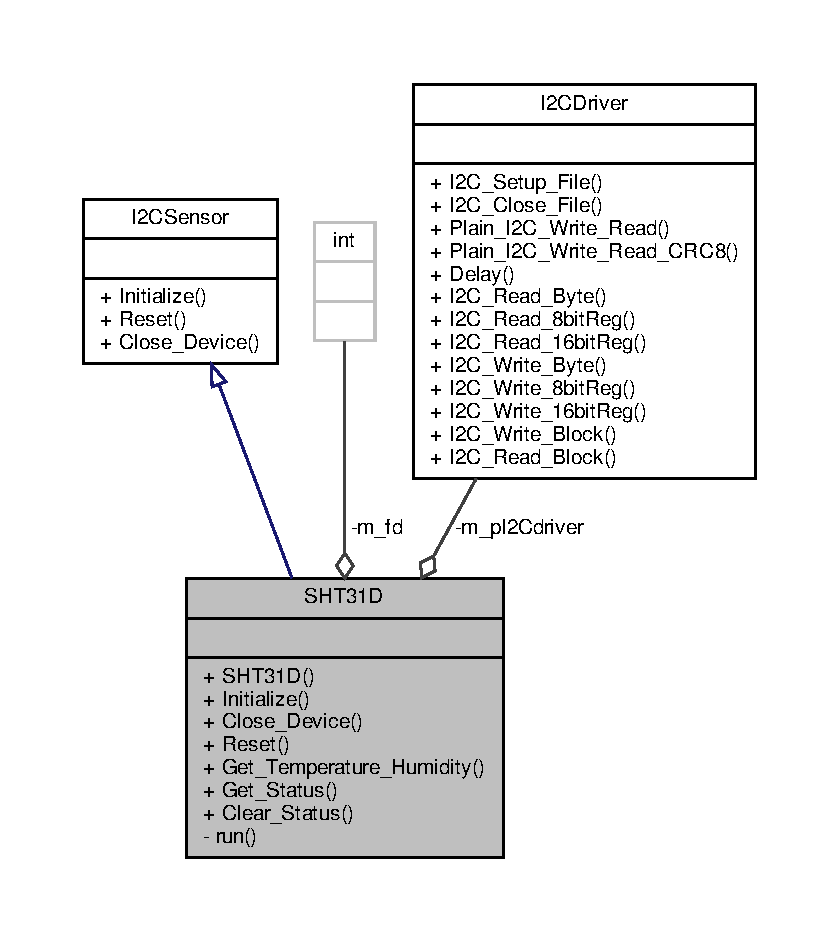
\includegraphics[width=350pt]{classSHT31D__coll__graph}
\end{center}
\end{figure}
\subsection*{Public Member Functions}
\begin{DoxyCompactItemize}
\item 
\hyperlink{classSHT31D_a697a7f48dbe4c821e81de47d8fbb2c74}{S\+H\+T31D} ()
\item 
int \hyperlink{classSHT31D_af3ec39a4f04344a1b422761cc904343e}{Initialize} (\hyperlink{classI2CDriver}{I2\+C\+Driver} \&i2c) override
\item 
int \hyperlink{classSHT31D_a925cd964b0a6535d40dff588ac7d02be}{Close\+\_\+\+Device} () override
\item 
int \hyperlink{classSHT31D_aa5d28c2557ed05435ca9b433492b9b07}{Reset} () override
\item 
int \hyperlink{classSHT31D_a749e5909bbd129e6352a32f28aef96d8}{Get\+\_\+\+Temperature\+\_\+\+Humidity} (float \&temperature, float \&humidity)
\item 
int \hyperlink{classSHT31D_ada8e1773dee18a8a76656bb2d41b19f1}{Get\+\_\+\+Status} (uint16\+\_\+t \&return\+Buffer)
\item 
int \hyperlink{classSHT31D_a29d822bbc17bae95b35270128942c2ba}{Clear\+\_\+\+Status} (void)
\end{DoxyCompactItemize}
\subsection*{Private Types}
\begin{DoxyCompactItemize}
\item 
enum \{ \hyperlink{classSHT31D_a5810e24af0e5737b6df24089366100fea7a00c3f8439a0de223d6fe77132acc69}{S\+H\+T31\+D\+\_\+\+I2\+C\+\_\+\+A\+D\+D\+R\+E\+SS} = 0x44
 \}
\item 
enum \{ \hyperlink{classSHT31D_abcfdc15982f0b22747afa7e3c325706aa4cdf0feb8a281e9ea9b49c913666f765}{S\+H\+T31\+D\+\_\+\+R\+E\+A\+D\+\_\+\+S\+E\+R\+I\+A\+L\+NO} = 0x3780
 \}
\item 
enum \{ \hyperlink{classSHT31D_aff87615787f9fd6f287b22b5f407d222a8a5caa21d4686c35ce1b7ff092c8f01d}{S\+H\+T31\+D\+\_\+\+M\+E\+A\+S\+\_\+\+M\+E\+D\+R\+EP} = 0x240B
 \}
\item 
enum \{ \hyperlink{classSHT31D_a72375ee81208748cd053d13a256c25cda0c1298490bd20d683dd0a189d1f33f80}{S\+H\+T31\+D\+\_\+\+R\+E\+A\+D\+\_\+\+S\+T\+A\+T\+US} = 0x\+F32D
 \}
\item 
enum \{ \hyperlink{classSHT31D_a40c567ed542f06f8cc22db0764415419ab93931def2227da6c7bcb0ec8d2ac171}{S\+H\+T31\+D\+\_\+\+C\+L\+E\+A\+R\+\_\+\+S\+T\+A\+T\+US} = 0x3041
 \}
\item 
enum \{ \hyperlink{classSHT31D_ae72fd59d3f80785321012a7d001a9008a8143b8b9241db83920c6fe106b9b787a}{S\+H\+T31\+D\+\_\+\+S\+O\+F\+T\+\_\+\+R\+E\+S\+ET} = 0x30\+A2
 \}
\end{DoxyCompactItemize}
\subsection*{Private Member Functions}
\begin{DoxyCompactItemize}
\item 
void \hyperlink{classSHT31D_a1cb98e435a44e2b6beeb3d0226cc9ec8}{run} ()
\end{DoxyCompactItemize}
\subsection*{Private Attributes}
\begin{DoxyCompactItemize}
\item 
int \hyperlink{classSHT31D_a2740f957337c1944421401643a6a15b6}{m\+\_\+fd}
\item 
\hyperlink{classI2CDriver}{I2\+C\+Driver} $\ast$ \hyperlink{classSHT31D_ad76767dc72097d43aea68675ae33e1ed}{m\+\_\+p\+I2\+Cdriver} = nullptr
\end{DoxyCompactItemize}


\subsection{Detailed Description}
\hyperlink{classSHT31D}{S\+H\+T31D} class. 

\begin{DoxyAuthor}{Author}
Kamil Rog
\end{DoxyAuthor}
This is class is responsilbe for the \hyperlink{classSHT31D}{S\+H\+T31D} temperature and humidity sensor.

P\+R\+O\+T\+O\+C\+OL -\/ I2C 

\subsection{Member Enumeration Documentation}
\mbox{\Hypertarget{classSHT31D_a5810e24af0e5737b6df24089366100fe}\label{classSHT31D_a5810e24af0e5737b6df24089366100fe}} 
\subsubsection{\texorpdfstring{anonymous enum}{anonymous enum}}
{\footnotesize\ttfamily anonymous enum\hspace{0.3cm}{\ttfamily [private]}}

\begin{DoxyEnumFields}{Enumerator}
\raisebox{\heightof{T}}[0pt][0pt]{\index{S\+H\+T31\+D\+\_\+\+I2\+C\+\_\+\+A\+D\+D\+R\+E\+SS@{S\+H\+T31\+D\+\_\+\+I2\+C\+\_\+\+A\+D\+D\+R\+E\+SS}!S\+H\+T31D@{S\+H\+T31D}}\index{S\+H\+T31D@{S\+H\+T31D}!S\+H\+T31\+D\+\_\+\+I2\+C\+\_\+\+A\+D\+D\+R\+E\+SS@{S\+H\+T31\+D\+\_\+\+I2\+C\+\_\+\+A\+D\+D\+R\+E\+SS}}}\mbox{\Hypertarget{classSHT31D_a5810e24af0e5737b6df24089366100fea7a00c3f8439a0de223d6fe77132acc69}\label{classSHT31D_a5810e24af0e5737b6df24089366100fea7a00c3f8439a0de223d6fe77132acc69}} 
S\+H\+T31\+D\+\_\+\+I2\+C\+\_\+\+A\+D\+D\+R\+E\+SS&\\
\hline

\end{DoxyEnumFields}
\mbox{\Hypertarget{classSHT31D_abcfdc15982f0b22747afa7e3c325706a}\label{classSHT31D_abcfdc15982f0b22747afa7e3c325706a}} 
\subsubsection{\texorpdfstring{anonymous enum}{anonymous enum}}
{\footnotesize\ttfamily anonymous enum\hspace{0.3cm}{\ttfamily [private]}}

\begin{DoxyEnumFields}{Enumerator}
\raisebox{\heightof{T}}[0pt][0pt]{\index{S\+H\+T31\+D\+\_\+\+R\+E\+A\+D\+\_\+\+S\+E\+R\+I\+A\+L\+NO@{S\+H\+T31\+D\+\_\+\+R\+E\+A\+D\+\_\+\+S\+E\+R\+I\+A\+L\+NO}!S\+H\+T31D@{S\+H\+T31D}}\index{S\+H\+T31D@{S\+H\+T31D}!S\+H\+T31\+D\+\_\+\+R\+E\+A\+D\+\_\+\+S\+E\+R\+I\+A\+L\+NO@{S\+H\+T31\+D\+\_\+\+R\+E\+A\+D\+\_\+\+S\+E\+R\+I\+A\+L\+NO}}}\mbox{\Hypertarget{classSHT31D_abcfdc15982f0b22747afa7e3c325706aa4cdf0feb8a281e9ea9b49c913666f765}\label{classSHT31D_abcfdc15982f0b22747afa7e3c325706aa4cdf0feb8a281e9ea9b49c913666f765}} 
S\+H\+T31\+D\+\_\+\+R\+E\+A\+D\+\_\+\+S\+E\+R\+I\+A\+L\+NO&\\
\hline

\end{DoxyEnumFields}
\mbox{\Hypertarget{classSHT31D_aff87615787f9fd6f287b22b5f407d222}\label{classSHT31D_aff87615787f9fd6f287b22b5f407d222}} 
\subsubsection{\texorpdfstring{anonymous enum}{anonymous enum}}
{\footnotesize\ttfamily anonymous enum\hspace{0.3cm}{\ttfamily [private]}}

\begin{DoxyEnumFields}{Enumerator}
\raisebox{\heightof{T}}[0pt][0pt]{\index{S\+H\+T31\+D\+\_\+\+M\+E\+A\+S\+\_\+\+M\+E\+D\+R\+EP@{S\+H\+T31\+D\+\_\+\+M\+E\+A\+S\+\_\+\+M\+E\+D\+R\+EP}!S\+H\+T31D@{S\+H\+T31D}}\index{S\+H\+T31D@{S\+H\+T31D}!S\+H\+T31\+D\+\_\+\+M\+E\+A\+S\+\_\+\+M\+E\+D\+R\+EP@{S\+H\+T31\+D\+\_\+\+M\+E\+A\+S\+\_\+\+M\+E\+D\+R\+EP}}}\mbox{\Hypertarget{classSHT31D_aff87615787f9fd6f287b22b5f407d222a8a5caa21d4686c35ce1b7ff092c8f01d}\label{classSHT31D_aff87615787f9fd6f287b22b5f407d222a8a5caa21d4686c35ce1b7ff092c8f01d}} 
S\+H\+T31\+D\+\_\+\+M\+E\+A\+S\+\_\+\+M\+E\+D\+R\+EP&\\
\hline

\end{DoxyEnumFields}
\mbox{\Hypertarget{classSHT31D_a72375ee81208748cd053d13a256c25cd}\label{classSHT31D_a72375ee81208748cd053d13a256c25cd}} 
\subsubsection{\texorpdfstring{anonymous enum}{anonymous enum}}
{\footnotesize\ttfamily anonymous enum\hspace{0.3cm}{\ttfamily [private]}}

\begin{DoxyEnumFields}{Enumerator}
\raisebox{\heightof{T}}[0pt][0pt]{\index{S\+H\+T31\+D\+\_\+\+R\+E\+A\+D\+\_\+\+S\+T\+A\+T\+US@{S\+H\+T31\+D\+\_\+\+R\+E\+A\+D\+\_\+\+S\+T\+A\+T\+US}!S\+H\+T31D@{S\+H\+T31D}}\index{S\+H\+T31D@{S\+H\+T31D}!S\+H\+T31\+D\+\_\+\+R\+E\+A\+D\+\_\+\+S\+T\+A\+T\+US@{S\+H\+T31\+D\+\_\+\+R\+E\+A\+D\+\_\+\+S\+T\+A\+T\+US}}}\mbox{\Hypertarget{classSHT31D_a72375ee81208748cd053d13a256c25cda0c1298490bd20d683dd0a189d1f33f80}\label{classSHT31D_a72375ee81208748cd053d13a256c25cda0c1298490bd20d683dd0a189d1f33f80}} 
S\+H\+T31\+D\+\_\+\+R\+E\+A\+D\+\_\+\+S\+T\+A\+T\+US&\\
\hline

\end{DoxyEnumFields}
\mbox{\Hypertarget{classSHT31D_a40c567ed542f06f8cc22db0764415419}\label{classSHT31D_a40c567ed542f06f8cc22db0764415419}} 
\subsubsection{\texorpdfstring{anonymous enum}{anonymous enum}}
{\footnotesize\ttfamily anonymous enum\hspace{0.3cm}{\ttfamily [private]}}

\begin{DoxyEnumFields}{Enumerator}
\raisebox{\heightof{T}}[0pt][0pt]{\index{S\+H\+T31\+D\+\_\+\+C\+L\+E\+A\+R\+\_\+\+S\+T\+A\+T\+US@{S\+H\+T31\+D\+\_\+\+C\+L\+E\+A\+R\+\_\+\+S\+T\+A\+T\+US}!S\+H\+T31D@{S\+H\+T31D}}\index{S\+H\+T31D@{S\+H\+T31D}!S\+H\+T31\+D\+\_\+\+C\+L\+E\+A\+R\+\_\+\+S\+T\+A\+T\+US@{S\+H\+T31\+D\+\_\+\+C\+L\+E\+A\+R\+\_\+\+S\+T\+A\+T\+US}}}\mbox{\Hypertarget{classSHT31D_a40c567ed542f06f8cc22db0764415419ab93931def2227da6c7bcb0ec8d2ac171}\label{classSHT31D_a40c567ed542f06f8cc22db0764415419ab93931def2227da6c7bcb0ec8d2ac171}} 
S\+H\+T31\+D\+\_\+\+C\+L\+E\+A\+R\+\_\+\+S\+T\+A\+T\+US&\\
\hline

\end{DoxyEnumFields}
\mbox{\Hypertarget{classSHT31D_ae72fd59d3f80785321012a7d001a9008}\label{classSHT31D_ae72fd59d3f80785321012a7d001a9008}} 
\subsubsection{\texorpdfstring{anonymous enum}{anonymous enum}}
{\footnotesize\ttfamily anonymous enum\hspace{0.3cm}{\ttfamily [private]}}

\begin{DoxyEnumFields}{Enumerator}
\raisebox{\heightof{T}}[0pt][0pt]{\index{S\+H\+T31\+D\+\_\+\+S\+O\+F\+T\+\_\+\+R\+E\+S\+ET@{S\+H\+T31\+D\+\_\+\+S\+O\+F\+T\+\_\+\+R\+E\+S\+ET}!S\+H\+T31D@{S\+H\+T31D}}\index{S\+H\+T31D@{S\+H\+T31D}!S\+H\+T31\+D\+\_\+\+S\+O\+F\+T\+\_\+\+R\+E\+S\+ET@{S\+H\+T31\+D\+\_\+\+S\+O\+F\+T\+\_\+\+R\+E\+S\+ET}}}\mbox{\Hypertarget{classSHT31D_ae72fd59d3f80785321012a7d001a9008a8143b8b9241db83920c6fe106b9b787a}\label{classSHT31D_ae72fd59d3f80785321012a7d001a9008a8143b8b9241db83920c6fe106b9b787a}} 
S\+H\+T31\+D\+\_\+\+S\+O\+F\+T\+\_\+\+R\+E\+S\+ET&\\
\hline

\end{DoxyEnumFields}


\subsection{Constructor \& Destructor Documentation}
\mbox{\Hypertarget{classSHT31D_a697a7f48dbe4c821e81de47d8fbb2c74}\label{classSHT31D_a697a7f48dbe4c821e81de47d8fbb2c74}} 
\index{S\+H\+T31D@{S\+H\+T31D}!S\+H\+T31D@{S\+H\+T31D}}
\index{S\+H\+T31D@{S\+H\+T31D}!S\+H\+T31D@{S\+H\+T31D}}
\subsubsection{\texorpdfstring{S\+H\+T31\+D()}{SHT31D()}}
{\footnotesize\ttfamily S\+H\+T31\+D\+::\+S\+H\+T31D (\begin{DoxyParamCaption}{ }\end{DoxyParamCaption})\hspace{0.3cm}{\ttfamily [inline]}}



\subsection{Member Function Documentation}
\mbox{\Hypertarget{classSHT31D_a29d822bbc17bae95b35270128942c2ba}\label{classSHT31D_a29d822bbc17bae95b35270128942c2ba}} 
\index{S\+H\+T31D@{S\+H\+T31D}!Clear\+\_\+\+Status@{Clear\+\_\+\+Status}}
\index{Clear\+\_\+\+Status@{Clear\+\_\+\+Status}!S\+H\+T31D@{S\+H\+T31D}}
\subsubsection{\texorpdfstring{Clear\+\_\+\+Status()}{Clear\_Status()}}
{\footnotesize\ttfamily int S\+H\+T31\+D\+::\+Clear\+\_\+\+Status (\begin{DoxyParamCaption}\item[{void}]{ }\end{DoxyParamCaption})}

Clears status

\begin{DoxyReturn}{Returns}
Zero on success else negative error number 
\end{DoxyReturn}
\mbox{\Hypertarget{classSHT31D_a925cd964b0a6535d40dff588ac7d02be}\label{classSHT31D_a925cd964b0a6535d40dff588ac7d02be}} 
\index{S\+H\+T31D@{S\+H\+T31D}!Close\+\_\+\+Device@{Close\+\_\+\+Device}}
\index{Close\+\_\+\+Device@{Close\+\_\+\+Device}!S\+H\+T31D@{S\+H\+T31D}}
\subsubsection{\texorpdfstring{Close\+\_\+\+Device()}{Close\_Device()}}
{\footnotesize\ttfamily int S\+H\+T31\+D\+::\+Close\+\_\+\+Device (\begin{DoxyParamCaption}\item[{void}]{ }\end{DoxyParamCaption})\hspace{0.3cm}{\ttfamily [override]}, {\ttfamily [virtual]}}

Close \hyperlink{classSHT31D}{S\+H\+T31D} file descriptor

\begin{DoxyReturn}{Returns}
None 
\end{DoxyReturn}


Implements \hyperlink{classI2CSensor_acee1633439e97bae412441ac085fabba}{I2\+C\+Sensor}.

\mbox{\Hypertarget{classSHT31D_ada8e1773dee18a8a76656bb2d41b19f1}\label{classSHT31D_ada8e1773dee18a8a76656bb2d41b19f1}} 
\index{S\+H\+T31D@{S\+H\+T31D}!Get\+\_\+\+Status@{Get\+\_\+\+Status}}
\index{Get\+\_\+\+Status@{Get\+\_\+\+Status}!S\+H\+T31D@{S\+H\+T31D}}
\subsubsection{\texorpdfstring{Get\+\_\+\+Status()}{Get\_Status()}}
{\footnotesize\ttfamily int S\+H\+T31\+D\+::\+Get\+\_\+\+Status (\begin{DoxyParamCaption}\item[{uint16\+\_\+t \&}]{status }\end{DoxyParamCaption})}

Get \hyperlink{classSHT31D}{S\+H\+T31D} Status


\begin{DoxyParams}{Parameters}
{\em status} & Address of status variable to update.\\
\hline
\end{DoxyParams}
\begin{DoxyReturn}{Returns}
Zero on success else negative error number 
\end{DoxyReturn}
\mbox{\Hypertarget{classSHT31D_a749e5909bbd129e6352a32f28aef96d8}\label{classSHT31D_a749e5909bbd129e6352a32f28aef96d8}} 
\index{S\+H\+T31D@{S\+H\+T31D}!Get\+\_\+\+Temperature\+\_\+\+Humidity@{Get\+\_\+\+Temperature\+\_\+\+Humidity}}
\index{Get\+\_\+\+Temperature\+\_\+\+Humidity@{Get\+\_\+\+Temperature\+\_\+\+Humidity}!S\+H\+T31D@{S\+H\+T31D}}
\subsubsection{\texorpdfstring{Get\+\_\+\+Temperature\+\_\+\+Humidity()}{Get\_Temperature\_Humidity()}}
{\footnotesize\ttfamily int S\+H\+T31\+D\+::\+Get\+\_\+\+Temperature\+\_\+\+Humidity (\begin{DoxyParamCaption}\item[{float \&}]{temperature,  }\item[{float \&}]{humidity }\end{DoxyParamCaption})}

Take a single Temperature \& Humidity measurement


\begin{DoxyParams}{Parameters}
{\em temperature} & Pointer to the temperature variable to modify. \\
\hline
{\em humidity} & Pointer to the humidity variable to modify\\
\hline
\end{DoxyParams}
\begin{DoxyReturn}{Returns}
Zero on success else negative error number 
\end{DoxyReturn}
\mbox{\Hypertarget{classSHT31D_af3ec39a4f04344a1b422761cc904343e}\label{classSHT31D_af3ec39a4f04344a1b422761cc904343e}} 
\index{S\+H\+T31D@{S\+H\+T31D}!Initialize@{Initialize}}
\index{Initialize@{Initialize}!S\+H\+T31D@{S\+H\+T31D}}
\subsubsection{\texorpdfstring{Initialize()}{Initialize()}}
{\footnotesize\ttfamily int S\+H\+T31\+D\+::\+Initialize (\begin{DoxyParamCaption}\item[{\hyperlink{classI2CDriver}{I2\+C\+Driver} \&}]{i2c }\end{DoxyParamCaption})\hspace{0.3cm}{\ttfamily [override]}, {\ttfamily [virtual]}}

Initialize \hyperlink{classSHT31D}{S\+H\+T31D} Open file descriptor

\begin{DoxyReturn}{Returns}
None 
\end{DoxyReturn}


Implements \hyperlink{classI2CSensor_a0fb4755ddff3fe2cf5a9651d9d1fe5cd}{I2\+C\+Sensor}.

\mbox{\Hypertarget{classSHT31D_aa5d28c2557ed05435ca9b433492b9b07}\label{classSHT31D_aa5d28c2557ed05435ca9b433492b9b07}} 
\index{S\+H\+T31D@{S\+H\+T31D}!Reset@{Reset}}
\index{Reset@{Reset}!S\+H\+T31D@{S\+H\+T31D}}
\subsubsection{\texorpdfstring{Reset()}{Reset()}}
{\footnotesize\ttfamily int S\+H\+T31\+D\+::\+Reset (\begin{DoxyParamCaption}\item[{void}]{ }\end{DoxyParamCaption})\hspace{0.3cm}{\ttfamily [override]}, {\ttfamily [virtual]}}

Soft Reset

\begin{DoxyReturn}{Returns}
Zero on success else negative error number 
\end{DoxyReturn}


Implements \hyperlink{classI2CSensor_a0622266d335944782d2bfa6352f01095}{I2\+C\+Sensor}.

\mbox{\Hypertarget{classSHT31D_a1cb98e435a44e2b6beeb3d0226cc9ec8}\label{classSHT31D_a1cb98e435a44e2b6beeb3d0226cc9ec8}} 
\index{S\+H\+T31D@{S\+H\+T31D}!run@{run}}
\index{run@{run}!S\+H\+T31D@{S\+H\+T31D}}
\subsubsection{\texorpdfstring{run()}{run()}}
{\footnotesize\ttfamily void S\+H\+T31\+D\+::run (\begin{DoxyParamCaption}{ }\end{DoxyParamCaption})\hspace{0.3cm}{\ttfamily [private]}}



\subsection{Member Data Documentation}
\mbox{\Hypertarget{classSHT31D_a2740f957337c1944421401643a6a15b6}\label{classSHT31D_a2740f957337c1944421401643a6a15b6}} 
\index{S\+H\+T31D@{S\+H\+T31D}!m\+\_\+fd@{m\+\_\+fd}}
\index{m\+\_\+fd@{m\+\_\+fd}!S\+H\+T31D@{S\+H\+T31D}}
\subsubsection{\texorpdfstring{m\+\_\+fd}{m\_fd}}
{\footnotesize\ttfamily int S\+H\+T31\+D\+::m\+\_\+fd\hspace{0.3cm}{\ttfamily [private]}}

\mbox{\Hypertarget{classSHT31D_ad76767dc72097d43aea68675ae33e1ed}\label{classSHT31D_ad76767dc72097d43aea68675ae33e1ed}} 
\index{S\+H\+T31D@{S\+H\+T31D}!m\+\_\+p\+I2\+Cdriver@{m\+\_\+p\+I2\+Cdriver}}
\index{m\+\_\+p\+I2\+Cdriver@{m\+\_\+p\+I2\+Cdriver}!S\+H\+T31D@{S\+H\+T31D}}
\subsubsection{\texorpdfstring{m\+\_\+p\+I2\+Cdriver}{m\_pI2Cdriver}}
{\footnotesize\ttfamily \hyperlink{classI2CDriver}{I2\+C\+Driver}$\ast$ S\+H\+T31\+D\+::m\+\_\+p\+I2\+Cdriver = nullptr\hspace{0.3cm}{\ttfamily [private]}}



The documentation for this class was generated from the following files\+:\begin{DoxyCompactItemize}
\item 
src/controller/peripherials/\hyperlink{SHT31D_8h}{S\+H\+T31\+D.\+h}\item 
src/controller/peripherials/\hyperlink{SHT31D_8cpp}{S\+H\+T31\+D.\+cpp}\end{DoxyCompactItemize}

\hypertarget{structTargetEnvironmentData}{}\section{Target\+Environment\+Data Struct Reference}
\label{structTargetEnvironmentData}\index{Target\+Environment\+Data@{Target\+Environment\+Data}}


{\ttfamily \#include $<$type\+Definitions.\+h$>$}



Collaboration diagram for Target\+Environment\+Data\+:\nopagebreak
\begin{figure}[H]
\begin{center}
\leavevmode
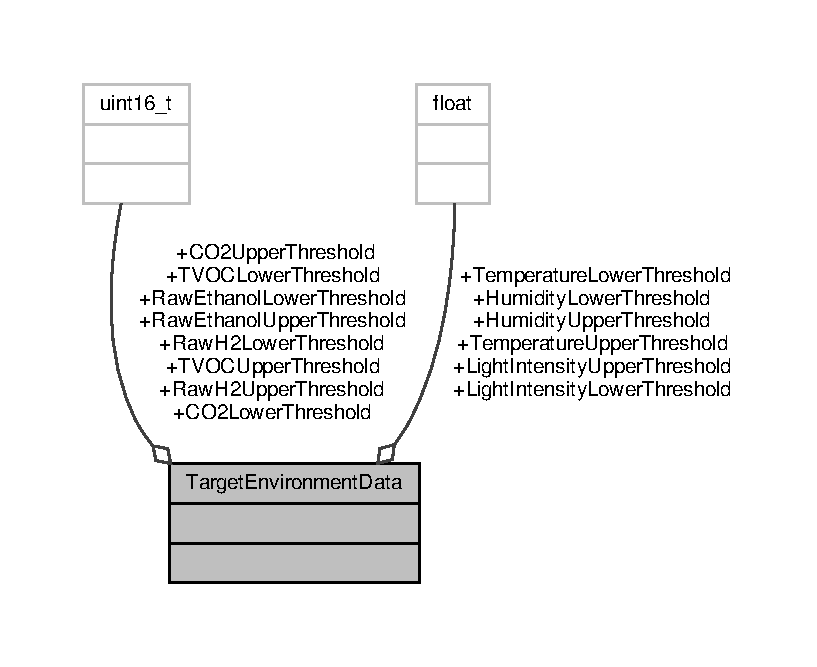
\includegraphics[width=350pt]{structTargetEnvironmentData__coll__graph}
\end{center}
\end{figure}
\subsection*{Public Attributes}
\begin{DoxyCompactItemize}
\item 
float \hyperlink{structTargetEnvironmentData_a7755db8c43daca465d5ac3730d57f7d8}{Light\+Intensity\+Upper\+Threshold}
\begin{DoxyCompactList}\small\item\em Alternativley use triple slash for the comments. \end{DoxyCompactList}\item 
float \hyperlink{structTargetEnvironmentData_a4619dffef19d60fd03d690fd756b595c}{Light\+Intensity\+Lower\+Threshold}
\item 
float \hyperlink{structTargetEnvironmentData_a76d83792b14767a1bc23b57c027232d6}{Temperature\+Upper\+Threshold}
\item 
float \hyperlink{structTargetEnvironmentData_a908d87e4fd88c513d671c591d0710ce0}{Temperature\+Lower\+Threshold}
\item 
float \hyperlink{structTargetEnvironmentData_a8db2e041382994d52fe089f9953ff437}{Humidity\+Upper\+Threshold}
\item 
float \hyperlink{structTargetEnvironmentData_af40ad465a6e74c13caf26b3672b7470f}{Humidity\+Lower\+Threshold}
\item 
uint16\+\_\+t \hyperlink{structTargetEnvironmentData_ae54690e5e73396443f43d3bbd9851d3c}{C\+O2\+Upper\+Threshold}
\item 
uint16\+\_\+t \hyperlink{structTargetEnvironmentData_a9584deda60eea2102608122a6ca6f791}{C\+O2\+Lower\+Threshold}
\item 
uint16\+\_\+t \hyperlink{structTargetEnvironmentData_afdddfbd81d51a1831704d85b08e9df1a}{T\+V\+O\+C\+Upper\+Threshold}
\item 
uint16\+\_\+t \hyperlink{structTargetEnvironmentData_a87019e6e28b712edf7900d6deef3e2b5}{T\+V\+O\+C\+Lower\+Threshold}
\item 
uint16\+\_\+t \hyperlink{structTargetEnvironmentData_ab0bb15f753619e3013f49dda97d15eab}{Raw\+Ethanol\+Upper\+Threshold}
\item 
uint16\+\_\+t \hyperlink{structTargetEnvironmentData_a113b5e5bcd192bcbdf5e845836c0be82}{Raw\+Ethanol\+Lower\+Threshold}
\item 
uint16\+\_\+t \hyperlink{structTargetEnvironmentData_a649b7d8751b329fba9494b5c730a55fd}{Raw\+H2\+Upper\+Threshold}
\item 
uint16\+\_\+t \hyperlink{structTargetEnvironmentData_abffe923b25c5ef2ccc1c9666c7397ed7}{Raw\+H2\+Lower\+Threshold}
\end{DoxyCompactItemize}


\subsection{Detailed Description}
Environment Data Struct Definition

This struct conatins all enviroment data read from sensors as well as target values 

\subsection{Member Data Documentation}
\mbox{\Hypertarget{structTargetEnvironmentData_a9584deda60eea2102608122a6ca6f791}\label{structTargetEnvironmentData_a9584deda60eea2102608122a6ca6f791}} 
\index{Target\+Environment\+Data@{Target\+Environment\+Data}!C\+O2\+Lower\+Threshold@{C\+O2\+Lower\+Threshold}}
\index{C\+O2\+Lower\+Threshold@{C\+O2\+Lower\+Threshold}!Target\+Environment\+Data@{Target\+Environment\+Data}}
\subsubsection{\texorpdfstring{C\+O2\+Lower\+Threshold}{CO2LowerThreshold}}
{\footnotesize\ttfamily uint16\+\_\+t Target\+Environment\+Data\+::\+C\+O2\+Lower\+Threshold}

Temperature of the envirnoment (in Degrees Celsius) \mbox{\Hypertarget{structTargetEnvironmentData_ae54690e5e73396443f43d3bbd9851d3c}\label{structTargetEnvironmentData_ae54690e5e73396443f43d3bbd9851d3c}} 
\index{Target\+Environment\+Data@{Target\+Environment\+Data}!C\+O2\+Upper\+Threshold@{C\+O2\+Upper\+Threshold}}
\index{C\+O2\+Upper\+Threshold@{C\+O2\+Upper\+Threshold}!Target\+Environment\+Data@{Target\+Environment\+Data}}
\subsubsection{\texorpdfstring{C\+O2\+Upper\+Threshold}{CO2UpperThreshold}}
{\footnotesize\ttfamily uint16\+\_\+t Target\+Environment\+Data\+::\+C\+O2\+Upper\+Threshold}

Temperature of the envirnoment (in Degrees Celsius) \mbox{\Hypertarget{structTargetEnvironmentData_af40ad465a6e74c13caf26b3672b7470f}\label{structTargetEnvironmentData_af40ad465a6e74c13caf26b3672b7470f}} 
\index{Target\+Environment\+Data@{Target\+Environment\+Data}!Humidity\+Lower\+Threshold@{Humidity\+Lower\+Threshold}}
\index{Humidity\+Lower\+Threshold@{Humidity\+Lower\+Threshold}!Target\+Environment\+Data@{Target\+Environment\+Data}}
\subsubsection{\texorpdfstring{Humidity\+Lower\+Threshold}{HumidityLowerThreshold}}
{\footnotesize\ttfamily float Target\+Environment\+Data\+::\+Humidity\+Lower\+Threshold}

Temperature of the envirnoment (in Degrees Celsius) \mbox{\Hypertarget{structTargetEnvironmentData_a8db2e041382994d52fe089f9953ff437}\label{structTargetEnvironmentData_a8db2e041382994d52fe089f9953ff437}} 
\index{Target\+Environment\+Data@{Target\+Environment\+Data}!Humidity\+Upper\+Threshold@{Humidity\+Upper\+Threshold}}
\index{Humidity\+Upper\+Threshold@{Humidity\+Upper\+Threshold}!Target\+Environment\+Data@{Target\+Environment\+Data}}
\subsubsection{\texorpdfstring{Humidity\+Upper\+Threshold}{HumidityUpperThreshold}}
{\footnotesize\ttfamily float Target\+Environment\+Data\+::\+Humidity\+Upper\+Threshold}

Temperature of the envirnoment (in Degrees Celsius) \mbox{\Hypertarget{structTargetEnvironmentData_a4619dffef19d60fd03d690fd756b595c}\label{structTargetEnvironmentData_a4619dffef19d60fd03d690fd756b595c}} 
\index{Target\+Environment\+Data@{Target\+Environment\+Data}!Light\+Intensity\+Lower\+Threshold@{Light\+Intensity\+Lower\+Threshold}}
\index{Light\+Intensity\+Lower\+Threshold@{Light\+Intensity\+Lower\+Threshold}!Target\+Environment\+Data@{Target\+Environment\+Data}}
\subsubsection{\texorpdfstring{Light\+Intensity\+Lower\+Threshold}{LightIntensityLowerThreshold}}
{\footnotesize\ttfamily float Target\+Environment\+Data\+::\+Light\+Intensity\+Lower\+Threshold}

Light Intensity of the envieronment (in Lux) \mbox{\Hypertarget{structTargetEnvironmentData_a7755db8c43daca465d5ac3730d57f7d8}\label{structTargetEnvironmentData_a7755db8c43daca465d5ac3730d57f7d8}} 
\index{Target\+Environment\+Data@{Target\+Environment\+Data}!Light\+Intensity\+Upper\+Threshold@{Light\+Intensity\+Upper\+Threshold}}
\index{Light\+Intensity\+Upper\+Threshold@{Light\+Intensity\+Upper\+Threshold}!Target\+Environment\+Data@{Target\+Environment\+Data}}
\subsubsection{\texorpdfstring{Light\+Intensity\+Upper\+Threshold}{LightIntensityUpperThreshold}}
{\footnotesize\ttfamily float Target\+Environment\+Data\+::\+Light\+Intensity\+Upper\+Threshold}



Alternativley use triple slash for the comments. 

Light Intensity of the envieronment (in Lux) \mbox{\Hypertarget{structTargetEnvironmentData_a113b5e5bcd192bcbdf5e845836c0be82}\label{structTargetEnvironmentData_a113b5e5bcd192bcbdf5e845836c0be82}} 
\index{Target\+Environment\+Data@{Target\+Environment\+Data}!Raw\+Ethanol\+Lower\+Threshold@{Raw\+Ethanol\+Lower\+Threshold}}
\index{Raw\+Ethanol\+Lower\+Threshold@{Raw\+Ethanol\+Lower\+Threshold}!Target\+Environment\+Data@{Target\+Environment\+Data}}
\subsubsection{\texorpdfstring{Raw\+Ethanol\+Lower\+Threshold}{RawEthanolLowerThreshold}}
{\footnotesize\ttfamily uint16\+\_\+t Target\+Environment\+Data\+::\+Raw\+Ethanol\+Lower\+Threshold}

Temperature of the envirnoment (in Degrees Celsius) \mbox{\Hypertarget{structTargetEnvironmentData_ab0bb15f753619e3013f49dda97d15eab}\label{structTargetEnvironmentData_ab0bb15f753619e3013f49dda97d15eab}} 
\index{Target\+Environment\+Data@{Target\+Environment\+Data}!Raw\+Ethanol\+Upper\+Threshold@{Raw\+Ethanol\+Upper\+Threshold}}
\index{Raw\+Ethanol\+Upper\+Threshold@{Raw\+Ethanol\+Upper\+Threshold}!Target\+Environment\+Data@{Target\+Environment\+Data}}
\subsubsection{\texorpdfstring{Raw\+Ethanol\+Upper\+Threshold}{RawEthanolUpperThreshold}}
{\footnotesize\ttfamily uint16\+\_\+t Target\+Environment\+Data\+::\+Raw\+Ethanol\+Upper\+Threshold}

Temperature of the envirnoment (in Degrees Celsius) \mbox{\Hypertarget{structTargetEnvironmentData_abffe923b25c5ef2ccc1c9666c7397ed7}\label{structTargetEnvironmentData_abffe923b25c5ef2ccc1c9666c7397ed7}} 
\index{Target\+Environment\+Data@{Target\+Environment\+Data}!Raw\+H2\+Lower\+Threshold@{Raw\+H2\+Lower\+Threshold}}
\index{Raw\+H2\+Lower\+Threshold@{Raw\+H2\+Lower\+Threshold}!Target\+Environment\+Data@{Target\+Environment\+Data}}
\subsubsection{\texorpdfstring{Raw\+H2\+Lower\+Threshold}{RawH2LowerThreshold}}
{\footnotesize\ttfamily uint16\+\_\+t Target\+Environment\+Data\+::\+Raw\+H2\+Lower\+Threshold}

Temperature of the envirnoment (in Degrees Celsius) \mbox{\Hypertarget{structTargetEnvironmentData_a649b7d8751b329fba9494b5c730a55fd}\label{structTargetEnvironmentData_a649b7d8751b329fba9494b5c730a55fd}} 
\index{Target\+Environment\+Data@{Target\+Environment\+Data}!Raw\+H2\+Upper\+Threshold@{Raw\+H2\+Upper\+Threshold}}
\index{Raw\+H2\+Upper\+Threshold@{Raw\+H2\+Upper\+Threshold}!Target\+Environment\+Data@{Target\+Environment\+Data}}
\subsubsection{\texorpdfstring{Raw\+H2\+Upper\+Threshold}{RawH2UpperThreshold}}
{\footnotesize\ttfamily uint16\+\_\+t Target\+Environment\+Data\+::\+Raw\+H2\+Upper\+Threshold}

Temperature of the envirnoment (in Degrees Celsius) \mbox{\Hypertarget{structTargetEnvironmentData_a908d87e4fd88c513d671c591d0710ce0}\label{structTargetEnvironmentData_a908d87e4fd88c513d671c591d0710ce0}} 
\index{Target\+Environment\+Data@{Target\+Environment\+Data}!Temperature\+Lower\+Threshold@{Temperature\+Lower\+Threshold}}
\index{Temperature\+Lower\+Threshold@{Temperature\+Lower\+Threshold}!Target\+Environment\+Data@{Target\+Environment\+Data}}
\subsubsection{\texorpdfstring{Temperature\+Lower\+Threshold}{TemperatureLowerThreshold}}
{\footnotesize\ttfamily float Target\+Environment\+Data\+::\+Temperature\+Lower\+Threshold}

Temperature of the envirnoment (in Degrees Celsius) \mbox{\Hypertarget{structTargetEnvironmentData_a76d83792b14767a1bc23b57c027232d6}\label{structTargetEnvironmentData_a76d83792b14767a1bc23b57c027232d6}} 
\index{Target\+Environment\+Data@{Target\+Environment\+Data}!Temperature\+Upper\+Threshold@{Temperature\+Upper\+Threshold}}
\index{Temperature\+Upper\+Threshold@{Temperature\+Upper\+Threshold}!Target\+Environment\+Data@{Target\+Environment\+Data}}
\subsubsection{\texorpdfstring{Temperature\+Upper\+Threshold}{TemperatureUpperThreshold}}
{\footnotesize\ttfamily float Target\+Environment\+Data\+::\+Temperature\+Upper\+Threshold}

Temperature of the envirnoment (in Degrees Celsius) \mbox{\Hypertarget{structTargetEnvironmentData_a87019e6e28b712edf7900d6deef3e2b5}\label{structTargetEnvironmentData_a87019e6e28b712edf7900d6deef3e2b5}} 
\index{Target\+Environment\+Data@{Target\+Environment\+Data}!T\+V\+O\+C\+Lower\+Threshold@{T\+V\+O\+C\+Lower\+Threshold}}
\index{T\+V\+O\+C\+Lower\+Threshold@{T\+V\+O\+C\+Lower\+Threshold}!Target\+Environment\+Data@{Target\+Environment\+Data}}
\subsubsection{\texorpdfstring{T\+V\+O\+C\+Lower\+Threshold}{TVOCLowerThreshold}}
{\footnotesize\ttfamily uint16\+\_\+t Target\+Environment\+Data\+::\+T\+V\+O\+C\+Lower\+Threshold}

Temperature of the envirnoment (in Degrees Celsius) \mbox{\Hypertarget{structTargetEnvironmentData_afdddfbd81d51a1831704d85b08e9df1a}\label{structTargetEnvironmentData_afdddfbd81d51a1831704d85b08e9df1a}} 
\index{Target\+Environment\+Data@{Target\+Environment\+Data}!T\+V\+O\+C\+Upper\+Threshold@{T\+V\+O\+C\+Upper\+Threshold}}
\index{T\+V\+O\+C\+Upper\+Threshold@{T\+V\+O\+C\+Upper\+Threshold}!Target\+Environment\+Data@{Target\+Environment\+Data}}
\subsubsection{\texorpdfstring{T\+V\+O\+C\+Upper\+Threshold}{TVOCUpperThreshold}}
{\footnotesize\ttfamily uint16\+\_\+t Target\+Environment\+Data\+::\+T\+V\+O\+C\+Upper\+Threshold}

Temperature of the envirnoment (in Degrees Celsius) 

The documentation for this struct was generated from the following file\+:\begin{DoxyCompactItemize}
\item 
src/utils/\hyperlink{typeDefinitions_8h}{type\+Definitions.\+h}\end{DoxyCompactItemize}

\hypertarget{classVEML7700}{}\section{V\+E\+M\+L7700 Class Reference}
\label{classVEML7700}\index{V\+E\+M\+L7700@{V\+E\+M\+L7700}}


\hyperlink{classVEML7700}{V\+E\+M\+L7700} class.  




{\ttfamily \#include $<$V\+E\+M\+L7700.\+h$>$}



Inheritance diagram for V\+E\+M\+L7700\+:\nopagebreak
\begin{figure}[H]
\begin{center}
\leavevmode
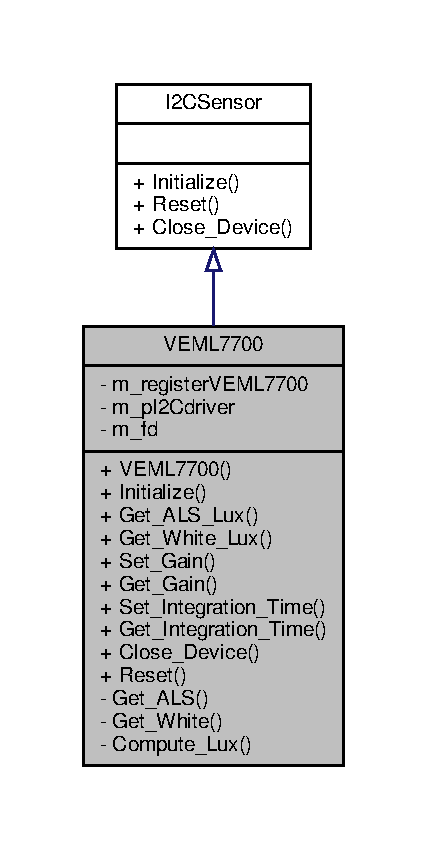
\includegraphics[width=205pt]{classVEML7700__inherit__graph}
\end{center}
\end{figure}


Collaboration diagram for V\+E\+M\+L7700\+:\nopagebreak
\begin{figure}[H]
\begin{center}
\leavevmode
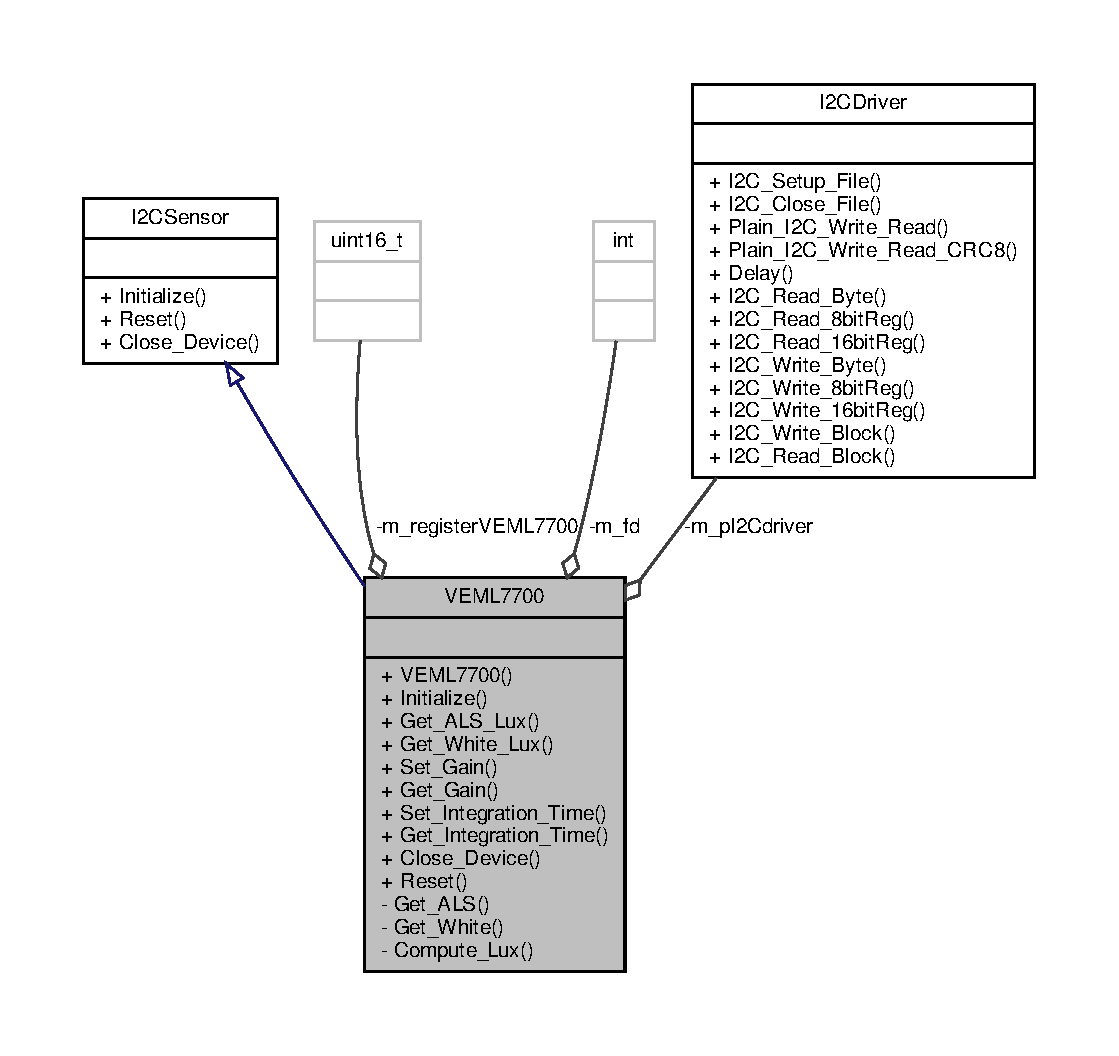
\includegraphics[width=350pt]{classVEML7700__coll__graph}
\end{center}
\end{figure}
\subsection*{Public Types}
\begin{DoxyCompactItemize}
\item 
enum \hyperlink{classVEML7700_a7328cc2563da545e48ea72381dc7bd9b}{A\+L\+S\+\_\+\+G\+A\+I\+N\+\_\+T} \{ \hyperlink{classVEML7700_a7328cc2563da545e48ea72381dc7bd9ba4c07a5980fa8aa1e6ea3e6e85a26eddf}{A\+L\+S\+\_\+\+G\+A\+I\+N\+\_\+x1} = 0x0, 
\hyperlink{classVEML7700_a7328cc2563da545e48ea72381dc7bd9ba80722e7850af774e558b2ef7684a81f4}{A\+L\+S\+\_\+\+G\+A\+I\+N\+\_\+x2} = 0x1, 
\hyperlink{classVEML7700_a7328cc2563da545e48ea72381dc7bd9ba393b9df437329457ca21bff810c8b7ee}{A\+L\+S\+\_\+\+G\+A\+I\+N\+\_\+d8} = 0x2, 
\hyperlink{classVEML7700_a7328cc2563da545e48ea72381dc7bd9ba0b5e6555c821a9c50adbe60629b15e4b}{A\+L\+S\+\_\+\+G\+A\+I\+N\+\_\+d4} = 0x3
 \}
\item 
enum \hyperlink{classVEML7700_a82e8b8f9960d8f80bc31dcfe7133ad6e}{A\+L\+S\+\_\+\+I\+N\+T\+E\+G\+R\+T\+A\+T\+I\+O\+N\+\_\+\+T\+I\+M\+E\+\_\+T} \{ \newline
\hyperlink{classVEML7700_a82e8b8f9960d8f80bc31dcfe7133ad6eac645a7593dba12a6d9410de0d7bd1703}{A\+L\+S\+\_\+\+I\+N\+T\+E\+G\+R\+A\+T\+I\+O\+N\+\_\+25ms} = 0xc, 
\hyperlink{classVEML7700_a82e8b8f9960d8f80bc31dcfe7133ad6eac1519635aa44f50fcc4ed955ad1c04e1}{A\+L\+S\+\_\+\+I\+N\+T\+E\+G\+R\+A\+T\+I\+O\+N\+\_\+50ms} = 0x8, 
\hyperlink{classVEML7700_a82e8b8f9960d8f80bc31dcfe7133ad6ea400cae3f071cb84b9eb779dae45e2f37}{A\+L\+S\+\_\+\+I\+N\+T\+E\+G\+R\+A\+T\+I\+O\+N\+\_\+100ms} = 0x0, 
\hyperlink{classVEML7700_a82e8b8f9960d8f80bc31dcfe7133ad6ea4907ac5a1fae354c96383c7f1a8b7aac}{A\+L\+S\+\_\+\+I\+N\+T\+E\+G\+R\+A\+T\+I\+O\+N\+\_\+200ms} = 0x1, 
\newline
\hyperlink{classVEML7700_a82e8b8f9960d8f80bc31dcfe7133ad6ea0d6e0a5191550c7983a5e6d3e4376495}{A\+L\+S\+\_\+\+I\+N\+T\+E\+G\+R\+A\+T\+I\+O\+N\+\_\+400ms} = 0x2, 
\hyperlink{classVEML7700_a82e8b8f9960d8f80bc31dcfe7133ad6eab6d8894bd9f6a20f4a9870751e572fda}{A\+L\+S\+\_\+\+I\+N\+T\+E\+G\+R\+A\+T\+I\+O\+N\+\_\+800ms} = 0x3
 \}
\item 
enum \hyperlink{classVEML7700_a4f3d9c3d3014149a380dabbf35decb3c}{A\+L\+S\+\_\+\+P\+E\+R\+S\+I\+S\+T\+E\+N\+C\+E\+\_\+T} \{ \hyperlink{classVEML7700_a4f3d9c3d3014149a380dabbf35decb3cace3cd89e100b478d3cce4c053e8d23e1}{A\+L\+S\+\_\+\+P\+E\+R\+S\+I\+S\+T\+E\+N\+C\+E\+\_\+1} = 0x0, 
\hyperlink{classVEML7700_a4f3d9c3d3014149a380dabbf35decb3ca7277f3289328bb4c176243aec5f6015b}{A\+L\+S\+\_\+\+P\+E\+R\+S\+I\+S\+T\+E\+N\+C\+E\+\_\+2} = 0x1, 
\hyperlink{classVEML7700_a4f3d9c3d3014149a380dabbf35decb3ca852553ed3cf1f1e0b972fab8899f032f}{A\+L\+S\+\_\+\+P\+E\+R\+S\+I\+S\+T\+E\+N\+C\+E\+\_\+4} = 0x2, 
\hyperlink{classVEML7700_a4f3d9c3d3014149a380dabbf35decb3cad5c65357a9ba8cc17a3b8b30169b9590}{A\+L\+S\+\_\+\+P\+E\+R\+S\+I\+S\+T\+E\+N\+C\+E\+\_\+8} = 0x3
 \}
\item 
enum \hyperlink{classVEML7700_ab2266ec2b4e62447d74a5dce5cc34282}{A\+L\+S\+\_\+\+P\+O\+W\+E\+R\+M\+O\+D\+E\+\_\+T} \{ \hyperlink{classVEML7700_ab2266ec2b4e62447d74a5dce5cc34282a65221f69f2af6a28d95bc4519664bf13}{A\+L\+S\+\_\+\+P\+O\+W\+E\+R\+\_\+\+M\+O\+D\+E\+\_\+1} = 0x0, 
\hyperlink{classVEML7700_ab2266ec2b4e62447d74a5dce5cc34282af10ede06dc073f78f7ca0ba2d98e3dfb}{A\+L\+S\+\_\+\+P\+O\+W\+E\+R\+\_\+\+M\+O\+D\+E\+\_\+2} = 0x1, 
\hyperlink{classVEML7700_ab2266ec2b4e62447d74a5dce5cc34282a6b6fde3da4b3e13b0c0207dc31d62e1b}{A\+L\+S\+\_\+\+P\+O\+W\+E\+R\+\_\+\+M\+O\+D\+E\+\_\+3} = 0x2, 
\hyperlink{classVEML7700_ab2266ec2b4e62447d74a5dce5cc34282aeb27a31fc102f1bfeb57a15726a71c51}{A\+L\+S\+\_\+\+P\+O\+W\+E\+R\+\_\+\+M\+O\+D\+E\+\_\+4} = 0x3
 \}
\end{DoxyCompactItemize}
\subsection*{Public Member Functions}
\begin{DoxyCompactItemize}
\item 
\hyperlink{classVEML7700_a6b351807d27da4e07ea3bb93bd3dcbb1}{V\+E\+M\+L7700} (void)
\item 
int \hyperlink{classVEML7700_af772ec5fe2bac04428479c9d232f1799}{Initialize} (\hyperlink{classI2CDriver}{I2\+C\+Driver} \&i2c) override
\item 
uint8\+\_\+t \hyperlink{classVEML7700_acf024ffb95cc98d82a708f511ec63d4e}{Get\+\_\+\+A\+L\+S\+\_\+\+Lux} (float \&lux)
\item 
uint8\+\_\+t \hyperlink{classVEML7700_a0f046c3327cac02f34cf9bfe2ac1231b}{Get\+\_\+\+White\+\_\+\+Lux} (float \&white)
\item 
uint8\+\_\+t \hyperlink{classVEML7700_aecbcabefbc9469ea91153723925acbd3}{Set\+\_\+\+Gain} (\hyperlink{classVEML7700_a7328cc2563da545e48ea72381dc7bd9b}{A\+L\+S\+\_\+\+G\+A\+I\+N\+\_\+T} gain)
\item 
uint8\+\_\+t \hyperlink{classVEML7700_a127d85c25f32b5bc0282fb04ad813fd6}{Get\+\_\+\+Gain} (\hyperlink{classVEML7700_a7328cc2563da545e48ea72381dc7bd9b}{A\+L\+S\+\_\+\+G\+A\+I\+N\+\_\+T} \&gain)
\item 
uint8\+\_\+t \hyperlink{classVEML7700_af3f3de94154ca1dd8905e932686ca23c}{Set\+\_\+\+Integration\+\_\+\+Time} (\hyperlink{classVEML7700_a82e8b8f9960d8f80bc31dcfe7133ad6e}{A\+L\+S\+\_\+\+I\+N\+T\+E\+G\+R\+T\+A\+T\+I\+O\+N\+\_\+\+T\+I\+M\+E\+\_\+T} integration\+Time)
\item 
uint8\+\_\+t \hyperlink{classVEML7700_a226efafb0bbc8068fbdf02f2d0afc0a0}{Get\+\_\+\+Integration\+\_\+\+Time} (\hyperlink{classVEML7700_a82e8b8f9960d8f80bc31dcfe7133ad6e}{A\+L\+S\+\_\+\+I\+N\+T\+E\+G\+R\+T\+A\+T\+I\+O\+N\+\_\+\+T\+I\+M\+E\+\_\+T} \&integration\+Time)
\item 
int \hyperlink{classVEML7700_af4be747d3c60af76ca46c7e4fb859ec7}{Close\+\_\+\+Device} () override
\item 
int \hyperlink{classVEML7700_a381358f8998260f4600a0d6713f7ea2a}{Reset} () override
\end{DoxyCompactItemize}
\subsection*{Private Types}
\begin{DoxyCompactItemize}
\item 
enum \{ \hyperlink{classVEML7700_ab63c7a3f732769f87046a7fe517fa5d2a89ac7a0c3d5299cc896db94f3f11ad3b}{I2\+C\+\_\+\+A\+D\+D\+R\+E\+SS} = 0x10
 \}
\item 
enum \{ \hyperlink{classVEML7700_a4173dfe44f2cce96da124bdecab4cea9a4f94aea0ea0bd1f3ddde34f141fb40b0}{C\+O\+M\+M\+A\+N\+D\+\_\+\+A\+L\+S\+\_\+\+SM} = 0x00, 
\hyperlink{classVEML7700_a4173dfe44f2cce96da124bdecab4cea9a0cc9ee77ebfb54f10e8e0b310557e8bc}{A\+L\+S\+\_\+\+S\+M\+\_\+\+M\+A\+SK} = 0x1800, 
\hyperlink{classVEML7700_a4173dfe44f2cce96da124bdecab4cea9a267f0498d6ffd9942d82af76204cdf94}{A\+L\+S\+\_\+\+S\+M\+\_\+\+S\+H\+I\+FT} = 11
 \}
\item 
enum \{ \hyperlink{classVEML7700_a8fc60ed332ae2b50905f477742e155c5ae6b6537105961e230f3c3bd922af64e7}{C\+O\+M\+M\+A\+N\+D\+\_\+\+A\+L\+S\+\_\+\+IT} = 0x00, 
\hyperlink{classVEML7700_a8fc60ed332ae2b50905f477742e155c5a3a76e5f3bed2f727dc77529203b4709d}{A\+L\+S\+\_\+\+I\+T\+\_\+\+M\+A\+SK} = 0x03c0, 
\hyperlink{classVEML7700_a8fc60ed332ae2b50905f477742e155c5a6a0ef54484f8ca1e5e9fc40e5268ea9b}{A\+L\+S\+\_\+\+I\+T\+\_\+\+S\+H\+I\+FT} = 6
 \}
\item 
enum \{ \hyperlink{classVEML7700_a29c6b040874a46d6911a8e78566057b7a4c3ed42cb54ed1d56e233cb2b63a7af9}{C\+O\+M\+M\+A\+N\+D\+\_\+\+A\+L\+S\+\_\+\+P\+E\+RS} = 0x00, 
\hyperlink{classVEML7700_a29c6b040874a46d6911a8e78566057b7a3e52078f4c2aa271762fa258b542756e}{A\+L\+S\+\_\+\+P\+E\+R\+S\+\_\+\+M\+A\+SK} = 0x0030, 
\hyperlink{classVEML7700_a29c6b040874a46d6911a8e78566057b7aac2f5794157be86c64a3304676a50801}{A\+L\+S\+\_\+\+P\+E\+R\+S\+\_\+\+S\+H\+I\+FT} = 4
 \}
\item 
enum \{ \hyperlink{classVEML7700_a6e9e3003ac094c096b9095a3ceb9faaeab1bae27fdd79e5fd8f79dfa27cbdb147}{C\+O\+M\+M\+A\+N\+D\+\_\+\+A\+L\+S\+\_\+\+I\+N\+T\+\_\+\+EN} = 0x00, 
\hyperlink{classVEML7700_a6e9e3003ac094c096b9095a3ceb9faaea6f3348962ed45d34cafcdeff49792472}{A\+L\+S\+\_\+\+I\+N\+T\+\_\+\+E\+N\+\_\+\+M\+A\+SK} = 0x0002, 
\hyperlink{classVEML7700_a6e9e3003ac094c096b9095a3ceb9faaea698db2febefb152579472c9aeee16f71}{A\+L\+S\+\_\+\+I\+N\+T\+\_\+\+E\+N\+\_\+\+S\+H\+I\+FT} = 1
 \}
\item 
enum \{ \hyperlink{classVEML7700_afba237ed01b4949e9aeb96151f9273b5ae4acf5f5dc8e4039bdc97cdb84c3d668}{C\+O\+M\+M\+A\+N\+D\+\_\+\+A\+L\+S\+\_\+\+SD} = 0x00, 
\hyperlink{classVEML7700_afba237ed01b4949e9aeb96151f9273b5a2fd5844c6a640f48b67c7bd56f2cc8c0}{A\+L\+S\+\_\+\+S\+D\+\_\+\+M\+A\+SK} = 0x0001, 
\hyperlink{classVEML7700_afba237ed01b4949e9aeb96151f9273b5a786e4e2edfd8bbe8e033a3aec13f410a}{A\+L\+S\+\_\+\+S\+D\+\_\+\+S\+H\+I\+FT} = 0
 \}
\item 
enum \{ \hyperlink{classVEML7700_af00a284cf91c8f469f2ff1af9805fdfbaf2d5b2cc1ae968d5228c83322be1ed9b}{C\+O\+M\+M\+A\+N\+D\+\_\+\+A\+L\+S\+\_\+\+WH} = 0x01
 \}
\item 
enum \{ \hyperlink{classVEML7700_a660a8a0b8955a6a316aa65fbceda8c0fa33d1cafd2cc649dfc04a2e5efdde55f7}{C\+O\+M\+M\+A\+N\+D\+\_\+\+A\+L\+S\+\_\+\+WL} = 0x02
 \}
\item 
enum \{ \hyperlink{classVEML7700_ab29ccdbcd4e170ac8663965e40523012a10105e35082facc6bce9f96ce60e0113}{C\+O\+M\+M\+A\+N\+D\+\_\+\+P\+SM} = 0x03, 
\hyperlink{classVEML7700_ab29ccdbcd4e170ac8663965e40523012a0cf5a09e1bd111e893e0cfc535c227dc}{P\+S\+M\+\_\+\+M\+A\+SK} = 0x0006, 
\hyperlink{classVEML7700_ab29ccdbcd4e170ac8663965e40523012a100f7cf3af8443f352a3030a062e5d17}{P\+S\+M\+\_\+\+S\+H\+I\+FT} = 1
 \}
\item 
enum \{ \hyperlink{classVEML7700_ab9eb0034cdb5c017a8fab52a50390bafa8222ed77749165e06f68103b1908a0ab}{C\+O\+M\+M\+A\+N\+D\+\_\+\+P\+S\+M\+\_\+\+EN} = 0x03, 
\hyperlink{classVEML7700_ab9eb0034cdb5c017a8fab52a50390bafa4430a48be44ce68abe4f34c61340af33}{P\+S\+M\+\_\+\+E\+N\+\_\+\+M\+A\+SK} = 0x0001, 
\hyperlink{classVEML7700_ab9eb0034cdb5c017a8fab52a50390bafaff513cb99fc1bd99f06cf6ed064e3750}{P\+S\+M\+\_\+\+E\+N\+\_\+\+S\+H\+I\+FT} = 0
 \}
\item 
enum \{ \hyperlink{classVEML7700_a2b96be5d4a52744ab8cfa400b4bbd623a0b4d97d359ebed7dda6535f1fdf29887}{C\+O\+M\+M\+A\+N\+D\+\_\+\+A\+LS} = 0x04
 \}
\item 
enum \{ \hyperlink{classVEML7700_addfea724a5192296d3dcc9392e420d0aa45821ad771eb9fdf961211ef411c861d}{C\+O\+M\+M\+A\+N\+D\+\_\+\+W\+H\+I\+TE} = 0x05
 \}
\item 
enum \{ \hyperlink{classVEML7700_a97d56ee9f3e176b36b73d4da40fa3d4aaeb3f59e8f54b7e72689ee0f25ed79307}{C\+O\+M\+M\+A\+N\+D\+\_\+\+A\+L\+S\+\_\+\+I\+F\+\_\+L} = 0x06, 
\hyperlink{classVEML7700_a97d56ee9f3e176b36b73d4da40fa3d4aa806747ccccccd1853f97cccc26151ff1}{A\+L\+S\+\_\+\+I\+F\+\_\+\+L\+\_\+\+M\+A\+SK} = 0x8000, 
\hyperlink{classVEML7700_a97d56ee9f3e176b36b73d4da40fa3d4aa236cddac0f7c78f37a578436901bcb68}{A\+L\+S\+\_\+\+I\+F\+\_\+\+L\+\_\+\+S\+H\+I\+FT} = 15
 \}
\item 
enum \{ \hyperlink{classVEML7700_afecc79a3882992a337dcb7fbd0f29b9ba2ddb21b523a11128c8b09fb056ec6e26}{C\+O\+M\+M\+A\+N\+D\+\_\+\+A\+L\+S\+\_\+\+I\+F\+\_\+H} = 0x06, 
\hyperlink{classVEML7700_afecc79a3882992a337dcb7fbd0f29b9ba1d0aa5abc421a84af1f7b07a1af45fd7}{A\+L\+S\+\_\+\+I\+F\+\_\+\+H\+\_\+\+M\+A\+SK} = 0x4000, 
\hyperlink{classVEML7700_afecc79a3882992a337dcb7fbd0f29b9ba27a522f8d1bc1192f2902c03a913137d}{A\+L\+S\+\_\+\+I\+F\+\_\+\+H\+\_\+\+S\+H\+I\+FT} = 14
 \}
\end{DoxyCompactItemize}
\subsection*{Private Member Functions}
\begin{DoxyCompactItemize}
\item 
uint8\+\_\+t \hyperlink{classVEML7700_a6a5e3bcbf41bc103823ca4d9f26ce31f}{Get\+\_\+\+A\+LS} (uint16\+\_\+t \&als)
\item 
uint8\+\_\+t \hyperlink{classVEML7700_aaee2f4b39b9391548ccb96bcdaebe2a0}{Get\+\_\+\+White} (uint16\+\_\+t \&white)
\item 
void \hyperlink{classVEML7700_a1e7056289f5d716f0d120cc5798d664a}{Compute\+\_\+\+Lux} (uint16\+\_\+t raw\+\_\+counts, float \&lux)
\end{DoxyCompactItemize}
\subsection*{Private Attributes}
\begin{DoxyCompactItemize}
\item 
uint16\+\_\+t \hyperlink{classVEML7700_a8e5c194037bceb4544cc1a7b05f697bb}{m\+\_\+register\+V\+E\+M\+L7700} \mbox{[}4\mbox{]}
\item 
\hyperlink{classI2CDriver}{I2\+C\+Driver} $\ast$ \hyperlink{classVEML7700_a06777141dab95a6244cc75e97a66f238}{m\+\_\+p\+I2\+Cdriver} = nullptr
\item 
int \hyperlink{classVEML7700_ae6d0418ab65f7fdfb21079d8637334af}{m\+\_\+fd}
\end{DoxyCompactItemize}


\subsection{Detailed Description}
\hyperlink{classVEML7700}{V\+E\+M\+L7700} class. 

\begin{DoxyAuthor}{Author}
Kamil Rog
\end{DoxyAuthor}
This is class is responsilbe for the \hyperlink{classVEML7700}{V\+E\+M\+L7700} light sensor.

P\+R\+O\+T\+O\+C\+OL -\/ I2C\hypertarget{classVEML7700_VEML7700}{}\subsection{Registers}\label{classVEML7700_VEML7700}
C\+O\+N\+F\+I\+G\+U\+R\+A\+T\+I\+ON R\+E\+G\+I\+S\+T\+ER \#0

B\+IT $\vert$ R\+E\+G\+I\+S\+T\+ER N\+A\+ME $\vert$ D\+E\+S\+C\+R\+I\+P\+T\+I\+ON 15 \+: 13 $\vert$ Reserved $\vert$ Set 000b 12 \+: 11 $\vert$ A\+L\+S\+\_\+\+G\+A\+IN $\vert$ See Enums for options 10 $\vert$ Reserved $\vert$ Set 0b 9 \+: 6 $\vert$ A\+L\+S\+\_\+\+IT $\vert$ See Enums for options 3 \+: 2 $\vert$ Reserved $\vert$ Set 00b 1 $\vert$ A\+L\+S\+\_\+\+I\+N\+T\+\_\+\+EN $\vert$ See Enums for options 0 $\vert$ A\+L\+S\+\_\+\+SD $\vert$ See Enums for options

C\+O\+M\+M\+A\+ND R\+E\+G\+I\+S\+T\+ER 

\subsection{Member Enumeration Documentation}
\mbox{\Hypertarget{classVEML7700_ab63c7a3f732769f87046a7fe517fa5d2}\label{classVEML7700_ab63c7a3f732769f87046a7fe517fa5d2}} 
\subsubsection{\texorpdfstring{anonymous enum}{anonymous enum}}
{\footnotesize\ttfamily anonymous enum\hspace{0.3cm}{\ttfamily [private]}}

\begin{DoxyEnumFields}{Enumerator}
\raisebox{\heightof{T}}[0pt][0pt]{\index{I2\+C\+\_\+\+A\+D\+D\+R\+E\+SS@{I2\+C\+\_\+\+A\+D\+D\+R\+E\+SS}!V\+E\+M\+L7700@{V\+E\+M\+L7700}}\index{V\+E\+M\+L7700@{V\+E\+M\+L7700}!I2\+C\+\_\+\+A\+D\+D\+R\+E\+SS@{I2\+C\+\_\+\+A\+D\+D\+R\+E\+SS}}}\mbox{\Hypertarget{classVEML7700_ab63c7a3f732769f87046a7fe517fa5d2a89ac7a0c3d5299cc896db94f3f11ad3b}\label{classVEML7700_ab63c7a3f732769f87046a7fe517fa5d2a89ac7a0c3d5299cc896db94f3f11ad3b}} 
I2\+C\+\_\+\+A\+D\+D\+R\+E\+SS&\\
\hline

\end{DoxyEnumFields}
\mbox{\Hypertarget{classVEML7700_a4173dfe44f2cce96da124bdecab4cea9}\label{classVEML7700_a4173dfe44f2cce96da124bdecab4cea9}} 
\subsubsection{\texorpdfstring{anonymous enum}{anonymous enum}}
{\footnotesize\ttfamily anonymous enum\hspace{0.3cm}{\ttfamily [private]}}

\begin{DoxyEnumFields}{Enumerator}
\raisebox{\heightof{T}}[0pt][0pt]{\index{C\+O\+M\+M\+A\+N\+D\+\_\+\+A\+L\+S\+\_\+\+SM@{C\+O\+M\+M\+A\+N\+D\+\_\+\+A\+L\+S\+\_\+\+SM}!V\+E\+M\+L7700@{V\+E\+M\+L7700}}\index{V\+E\+M\+L7700@{V\+E\+M\+L7700}!C\+O\+M\+M\+A\+N\+D\+\_\+\+A\+L\+S\+\_\+\+SM@{C\+O\+M\+M\+A\+N\+D\+\_\+\+A\+L\+S\+\_\+\+SM}}}\mbox{\Hypertarget{classVEML7700_a4173dfe44f2cce96da124bdecab4cea9a4f94aea0ea0bd1f3ddde34f141fb40b0}\label{classVEML7700_a4173dfe44f2cce96da124bdecab4cea9a4f94aea0ea0bd1f3ddde34f141fb40b0}} 
C\+O\+M\+M\+A\+N\+D\+\_\+\+A\+L\+S\+\_\+\+SM&\\
\hline

\raisebox{\heightof{T}}[0pt][0pt]{\index{A\+L\+S\+\_\+\+S\+M\+\_\+\+M\+A\+SK@{A\+L\+S\+\_\+\+S\+M\+\_\+\+M\+A\+SK}!V\+E\+M\+L7700@{V\+E\+M\+L7700}}\index{V\+E\+M\+L7700@{V\+E\+M\+L7700}!A\+L\+S\+\_\+\+S\+M\+\_\+\+M\+A\+SK@{A\+L\+S\+\_\+\+S\+M\+\_\+\+M\+A\+SK}}}\mbox{\Hypertarget{classVEML7700_a4173dfe44f2cce96da124bdecab4cea9a0cc9ee77ebfb54f10e8e0b310557e8bc}\label{classVEML7700_a4173dfe44f2cce96da124bdecab4cea9a0cc9ee77ebfb54f10e8e0b310557e8bc}} 
A\+L\+S\+\_\+\+S\+M\+\_\+\+M\+A\+SK&\\
\hline

\raisebox{\heightof{T}}[0pt][0pt]{\index{A\+L\+S\+\_\+\+S\+M\+\_\+\+S\+H\+I\+FT@{A\+L\+S\+\_\+\+S\+M\+\_\+\+S\+H\+I\+FT}!V\+E\+M\+L7700@{V\+E\+M\+L7700}}\index{V\+E\+M\+L7700@{V\+E\+M\+L7700}!A\+L\+S\+\_\+\+S\+M\+\_\+\+S\+H\+I\+FT@{A\+L\+S\+\_\+\+S\+M\+\_\+\+S\+H\+I\+FT}}}\mbox{\Hypertarget{classVEML7700_a4173dfe44f2cce96da124bdecab4cea9a267f0498d6ffd9942d82af76204cdf94}\label{classVEML7700_a4173dfe44f2cce96da124bdecab4cea9a267f0498d6ffd9942d82af76204cdf94}} 
A\+L\+S\+\_\+\+S\+M\+\_\+\+S\+H\+I\+FT&\\
\hline

\end{DoxyEnumFields}
\mbox{\Hypertarget{classVEML7700_a8fc60ed332ae2b50905f477742e155c5}\label{classVEML7700_a8fc60ed332ae2b50905f477742e155c5}} 
\subsubsection{\texorpdfstring{anonymous enum}{anonymous enum}}
{\footnotesize\ttfamily anonymous enum\hspace{0.3cm}{\ttfamily [private]}}

\begin{DoxyEnumFields}{Enumerator}
\raisebox{\heightof{T}}[0pt][0pt]{\index{C\+O\+M\+M\+A\+N\+D\+\_\+\+A\+L\+S\+\_\+\+IT@{C\+O\+M\+M\+A\+N\+D\+\_\+\+A\+L\+S\+\_\+\+IT}!V\+E\+M\+L7700@{V\+E\+M\+L7700}}\index{V\+E\+M\+L7700@{V\+E\+M\+L7700}!C\+O\+M\+M\+A\+N\+D\+\_\+\+A\+L\+S\+\_\+\+IT@{C\+O\+M\+M\+A\+N\+D\+\_\+\+A\+L\+S\+\_\+\+IT}}}\mbox{\Hypertarget{classVEML7700_a8fc60ed332ae2b50905f477742e155c5ae6b6537105961e230f3c3bd922af64e7}\label{classVEML7700_a8fc60ed332ae2b50905f477742e155c5ae6b6537105961e230f3c3bd922af64e7}} 
C\+O\+M\+M\+A\+N\+D\+\_\+\+A\+L\+S\+\_\+\+IT&\\
\hline

\raisebox{\heightof{T}}[0pt][0pt]{\index{A\+L\+S\+\_\+\+I\+T\+\_\+\+M\+A\+SK@{A\+L\+S\+\_\+\+I\+T\+\_\+\+M\+A\+SK}!V\+E\+M\+L7700@{V\+E\+M\+L7700}}\index{V\+E\+M\+L7700@{V\+E\+M\+L7700}!A\+L\+S\+\_\+\+I\+T\+\_\+\+M\+A\+SK@{A\+L\+S\+\_\+\+I\+T\+\_\+\+M\+A\+SK}}}\mbox{\Hypertarget{classVEML7700_a8fc60ed332ae2b50905f477742e155c5a3a76e5f3bed2f727dc77529203b4709d}\label{classVEML7700_a8fc60ed332ae2b50905f477742e155c5a3a76e5f3bed2f727dc77529203b4709d}} 
A\+L\+S\+\_\+\+I\+T\+\_\+\+M\+A\+SK&\\
\hline

\raisebox{\heightof{T}}[0pt][0pt]{\index{A\+L\+S\+\_\+\+I\+T\+\_\+\+S\+H\+I\+FT@{A\+L\+S\+\_\+\+I\+T\+\_\+\+S\+H\+I\+FT}!V\+E\+M\+L7700@{V\+E\+M\+L7700}}\index{V\+E\+M\+L7700@{V\+E\+M\+L7700}!A\+L\+S\+\_\+\+I\+T\+\_\+\+S\+H\+I\+FT@{A\+L\+S\+\_\+\+I\+T\+\_\+\+S\+H\+I\+FT}}}\mbox{\Hypertarget{classVEML7700_a8fc60ed332ae2b50905f477742e155c5a6a0ef54484f8ca1e5e9fc40e5268ea9b}\label{classVEML7700_a8fc60ed332ae2b50905f477742e155c5a6a0ef54484f8ca1e5e9fc40e5268ea9b}} 
A\+L\+S\+\_\+\+I\+T\+\_\+\+S\+H\+I\+FT&\\
\hline

\end{DoxyEnumFields}
\mbox{\Hypertarget{classVEML7700_a29c6b040874a46d6911a8e78566057b7}\label{classVEML7700_a29c6b040874a46d6911a8e78566057b7}} 
\subsubsection{\texorpdfstring{anonymous enum}{anonymous enum}}
{\footnotesize\ttfamily anonymous enum\hspace{0.3cm}{\ttfamily [private]}}

\begin{DoxyEnumFields}{Enumerator}
\raisebox{\heightof{T}}[0pt][0pt]{\index{C\+O\+M\+M\+A\+N\+D\+\_\+\+A\+L\+S\+\_\+\+P\+E\+RS@{C\+O\+M\+M\+A\+N\+D\+\_\+\+A\+L\+S\+\_\+\+P\+E\+RS}!V\+E\+M\+L7700@{V\+E\+M\+L7700}}\index{V\+E\+M\+L7700@{V\+E\+M\+L7700}!C\+O\+M\+M\+A\+N\+D\+\_\+\+A\+L\+S\+\_\+\+P\+E\+RS@{C\+O\+M\+M\+A\+N\+D\+\_\+\+A\+L\+S\+\_\+\+P\+E\+RS}}}\mbox{\Hypertarget{classVEML7700_a29c6b040874a46d6911a8e78566057b7a4c3ed42cb54ed1d56e233cb2b63a7af9}\label{classVEML7700_a29c6b040874a46d6911a8e78566057b7a4c3ed42cb54ed1d56e233cb2b63a7af9}} 
C\+O\+M\+M\+A\+N\+D\+\_\+\+A\+L\+S\+\_\+\+P\+E\+RS&\\
\hline

\raisebox{\heightof{T}}[0pt][0pt]{\index{A\+L\+S\+\_\+\+P\+E\+R\+S\+\_\+\+M\+A\+SK@{A\+L\+S\+\_\+\+P\+E\+R\+S\+\_\+\+M\+A\+SK}!V\+E\+M\+L7700@{V\+E\+M\+L7700}}\index{V\+E\+M\+L7700@{V\+E\+M\+L7700}!A\+L\+S\+\_\+\+P\+E\+R\+S\+\_\+\+M\+A\+SK@{A\+L\+S\+\_\+\+P\+E\+R\+S\+\_\+\+M\+A\+SK}}}\mbox{\Hypertarget{classVEML7700_a29c6b040874a46d6911a8e78566057b7a3e52078f4c2aa271762fa258b542756e}\label{classVEML7700_a29c6b040874a46d6911a8e78566057b7a3e52078f4c2aa271762fa258b542756e}} 
A\+L\+S\+\_\+\+P\+E\+R\+S\+\_\+\+M\+A\+SK&\\
\hline

\raisebox{\heightof{T}}[0pt][0pt]{\index{A\+L\+S\+\_\+\+P\+E\+R\+S\+\_\+\+S\+H\+I\+FT@{A\+L\+S\+\_\+\+P\+E\+R\+S\+\_\+\+S\+H\+I\+FT}!V\+E\+M\+L7700@{V\+E\+M\+L7700}}\index{V\+E\+M\+L7700@{V\+E\+M\+L7700}!A\+L\+S\+\_\+\+P\+E\+R\+S\+\_\+\+S\+H\+I\+FT@{A\+L\+S\+\_\+\+P\+E\+R\+S\+\_\+\+S\+H\+I\+FT}}}\mbox{\Hypertarget{classVEML7700_a29c6b040874a46d6911a8e78566057b7aac2f5794157be86c64a3304676a50801}\label{classVEML7700_a29c6b040874a46d6911a8e78566057b7aac2f5794157be86c64a3304676a50801}} 
A\+L\+S\+\_\+\+P\+E\+R\+S\+\_\+\+S\+H\+I\+FT&\\
\hline

\end{DoxyEnumFields}
\mbox{\Hypertarget{classVEML7700_a6e9e3003ac094c096b9095a3ceb9faae}\label{classVEML7700_a6e9e3003ac094c096b9095a3ceb9faae}} 
\subsubsection{\texorpdfstring{anonymous enum}{anonymous enum}}
{\footnotesize\ttfamily anonymous enum\hspace{0.3cm}{\ttfamily [private]}}

\begin{DoxyEnumFields}{Enumerator}
\raisebox{\heightof{T}}[0pt][0pt]{\index{C\+O\+M\+M\+A\+N\+D\+\_\+\+A\+L\+S\+\_\+\+I\+N\+T\+\_\+\+EN@{C\+O\+M\+M\+A\+N\+D\+\_\+\+A\+L\+S\+\_\+\+I\+N\+T\+\_\+\+EN}!V\+E\+M\+L7700@{V\+E\+M\+L7700}}\index{V\+E\+M\+L7700@{V\+E\+M\+L7700}!C\+O\+M\+M\+A\+N\+D\+\_\+\+A\+L\+S\+\_\+\+I\+N\+T\+\_\+\+EN@{C\+O\+M\+M\+A\+N\+D\+\_\+\+A\+L\+S\+\_\+\+I\+N\+T\+\_\+\+EN}}}\mbox{\Hypertarget{classVEML7700_a6e9e3003ac094c096b9095a3ceb9faaeab1bae27fdd79e5fd8f79dfa27cbdb147}\label{classVEML7700_a6e9e3003ac094c096b9095a3ceb9faaeab1bae27fdd79e5fd8f79dfa27cbdb147}} 
C\+O\+M\+M\+A\+N\+D\+\_\+\+A\+L\+S\+\_\+\+I\+N\+T\+\_\+\+EN&\\
\hline

\raisebox{\heightof{T}}[0pt][0pt]{\index{A\+L\+S\+\_\+\+I\+N\+T\+\_\+\+E\+N\+\_\+\+M\+A\+SK@{A\+L\+S\+\_\+\+I\+N\+T\+\_\+\+E\+N\+\_\+\+M\+A\+SK}!V\+E\+M\+L7700@{V\+E\+M\+L7700}}\index{V\+E\+M\+L7700@{V\+E\+M\+L7700}!A\+L\+S\+\_\+\+I\+N\+T\+\_\+\+E\+N\+\_\+\+M\+A\+SK@{A\+L\+S\+\_\+\+I\+N\+T\+\_\+\+E\+N\+\_\+\+M\+A\+SK}}}\mbox{\Hypertarget{classVEML7700_a6e9e3003ac094c096b9095a3ceb9faaea6f3348962ed45d34cafcdeff49792472}\label{classVEML7700_a6e9e3003ac094c096b9095a3ceb9faaea6f3348962ed45d34cafcdeff49792472}} 
A\+L\+S\+\_\+\+I\+N\+T\+\_\+\+E\+N\+\_\+\+M\+A\+SK&\\
\hline

\raisebox{\heightof{T}}[0pt][0pt]{\index{A\+L\+S\+\_\+\+I\+N\+T\+\_\+\+E\+N\+\_\+\+S\+H\+I\+FT@{A\+L\+S\+\_\+\+I\+N\+T\+\_\+\+E\+N\+\_\+\+S\+H\+I\+FT}!V\+E\+M\+L7700@{V\+E\+M\+L7700}}\index{V\+E\+M\+L7700@{V\+E\+M\+L7700}!A\+L\+S\+\_\+\+I\+N\+T\+\_\+\+E\+N\+\_\+\+S\+H\+I\+FT@{A\+L\+S\+\_\+\+I\+N\+T\+\_\+\+E\+N\+\_\+\+S\+H\+I\+FT}}}\mbox{\Hypertarget{classVEML7700_a6e9e3003ac094c096b9095a3ceb9faaea698db2febefb152579472c9aeee16f71}\label{classVEML7700_a6e9e3003ac094c096b9095a3ceb9faaea698db2febefb152579472c9aeee16f71}} 
A\+L\+S\+\_\+\+I\+N\+T\+\_\+\+E\+N\+\_\+\+S\+H\+I\+FT&\\
\hline

\end{DoxyEnumFields}
\mbox{\Hypertarget{classVEML7700_afba237ed01b4949e9aeb96151f9273b5}\label{classVEML7700_afba237ed01b4949e9aeb96151f9273b5}} 
\subsubsection{\texorpdfstring{anonymous enum}{anonymous enum}}
{\footnotesize\ttfamily anonymous enum\hspace{0.3cm}{\ttfamily [private]}}

\begin{DoxyEnumFields}{Enumerator}
\raisebox{\heightof{T}}[0pt][0pt]{\index{C\+O\+M\+M\+A\+N\+D\+\_\+\+A\+L\+S\+\_\+\+SD@{C\+O\+M\+M\+A\+N\+D\+\_\+\+A\+L\+S\+\_\+\+SD}!V\+E\+M\+L7700@{V\+E\+M\+L7700}}\index{V\+E\+M\+L7700@{V\+E\+M\+L7700}!C\+O\+M\+M\+A\+N\+D\+\_\+\+A\+L\+S\+\_\+\+SD@{C\+O\+M\+M\+A\+N\+D\+\_\+\+A\+L\+S\+\_\+\+SD}}}\mbox{\Hypertarget{classVEML7700_afba237ed01b4949e9aeb96151f9273b5ae4acf5f5dc8e4039bdc97cdb84c3d668}\label{classVEML7700_afba237ed01b4949e9aeb96151f9273b5ae4acf5f5dc8e4039bdc97cdb84c3d668}} 
C\+O\+M\+M\+A\+N\+D\+\_\+\+A\+L\+S\+\_\+\+SD&\\
\hline

\raisebox{\heightof{T}}[0pt][0pt]{\index{A\+L\+S\+\_\+\+S\+D\+\_\+\+M\+A\+SK@{A\+L\+S\+\_\+\+S\+D\+\_\+\+M\+A\+SK}!V\+E\+M\+L7700@{V\+E\+M\+L7700}}\index{V\+E\+M\+L7700@{V\+E\+M\+L7700}!A\+L\+S\+\_\+\+S\+D\+\_\+\+M\+A\+SK@{A\+L\+S\+\_\+\+S\+D\+\_\+\+M\+A\+SK}}}\mbox{\Hypertarget{classVEML7700_afba237ed01b4949e9aeb96151f9273b5a2fd5844c6a640f48b67c7bd56f2cc8c0}\label{classVEML7700_afba237ed01b4949e9aeb96151f9273b5a2fd5844c6a640f48b67c7bd56f2cc8c0}} 
A\+L\+S\+\_\+\+S\+D\+\_\+\+M\+A\+SK&\\
\hline

\raisebox{\heightof{T}}[0pt][0pt]{\index{A\+L\+S\+\_\+\+S\+D\+\_\+\+S\+H\+I\+FT@{A\+L\+S\+\_\+\+S\+D\+\_\+\+S\+H\+I\+FT}!V\+E\+M\+L7700@{V\+E\+M\+L7700}}\index{V\+E\+M\+L7700@{V\+E\+M\+L7700}!A\+L\+S\+\_\+\+S\+D\+\_\+\+S\+H\+I\+FT@{A\+L\+S\+\_\+\+S\+D\+\_\+\+S\+H\+I\+FT}}}\mbox{\Hypertarget{classVEML7700_afba237ed01b4949e9aeb96151f9273b5a786e4e2edfd8bbe8e033a3aec13f410a}\label{classVEML7700_afba237ed01b4949e9aeb96151f9273b5a786e4e2edfd8bbe8e033a3aec13f410a}} 
A\+L\+S\+\_\+\+S\+D\+\_\+\+S\+H\+I\+FT&\\
\hline

\end{DoxyEnumFields}
\mbox{\Hypertarget{classVEML7700_af00a284cf91c8f469f2ff1af9805fdfb}\label{classVEML7700_af00a284cf91c8f469f2ff1af9805fdfb}} 
\subsubsection{\texorpdfstring{anonymous enum}{anonymous enum}}
{\footnotesize\ttfamily anonymous enum\hspace{0.3cm}{\ttfamily [private]}}

\begin{DoxyEnumFields}{Enumerator}
\raisebox{\heightof{T}}[0pt][0pt]{\index{C\+O\+M\+M\+A\+N\+D\+\_\+\+A\+L\+S\+\_\+\+WH@{C\+O\+M\+M\+A\+N\+D\+\_\+\+A\+L\+S\+\_\+\+WH}!V\+E\+M\+L7700@{V\+E\+M\+L7700}}\index{V\+E\+M\+L7700@{V\+E\+M\+L7700}!C\+O\+M\+M\+A\+N\+D\+\_\+\+A\+L\+S\+\_\+\+WH@{C\+O\+M\+M\+A\+N\+D\+\_\+\+A\+L\+S\+\_\+\+WH}}}\mbox{\Hypertarget{classVEML7700_af00a284cf91c8f469f2ff1af9805fdfbaf2d5b2cc1ae968d5228c83322be1ed9b}\label{classVEML7700_af00a284cf91c8f469f2ff1af9805fdfbaf2d5b2cc1ae968d5228c83322be1ed9b}} 
C\+O\+M\+M\+A\+N\+D\+\_\+\+A\+L\+S\+\_\+\+WH&\\
\hline

\end{DoxyEnumFields}
\mbox{\Hypertarget{classVEML7700_a660a8a0b8955a6a316aa65fbceda8c0f}\label{classVEML7700_a660a8a0b8955a6a316aa65fbceda8c0f}} 
\subsubsection{\texorpdfstring{anonymous enum}{anonymous enum}}
{\footnotesize\ttfamily anonymous enum\hspace{0.3cm}{\ttfamily [private]}}

\begin{DoxyEnumFields}{Enumerator}
\raisebox{\heightof{T}}[0pt][0pt]{\index{C\+O\+M\+M\+A\+N\+D\+\_\+\+A\+L\+S\+\_\+\+WL@{C\+O\+M\+M\+A\+N\+D\+\_\+\+A\+L\+S\+\_\+\+WL}!V\+E\+M\+L7700@{V\+E\+M\+L7700}}\index{V\+E\+M\+L7700@{V\+E\+M\+L7700}!C\+O\+M\+M\+A\+N\+D\+\_\+\+A\+L\+S\+\_\+\+WL@{C\+O\+M\+M\+A\+N\+D\+\_\+\+A\+L\+S\+\_\+\+WL}}}\mbox{\Hypertarget{classVEML7700_a660a8a0b8955a6a316aa65fbceda8c0fa33d1cafd2cc649dfc04a2e5efdde55f7}\label{classVEML7700_a660a8a0b8955a6a316aa65fbceda8c0fa33d1cafd2cc649dfc04a2e5efdde55f7}} 
C\+O\+M\+M\+A\+N\+D\+\_\+\+A\+L\+S\+\_\+\+WL&\\
\hline

\end{DoxyEnumFields}
\mbox{\Hypertarget{classVEML7700_ab29ccdbcd4e170ac8663965e40523012}\label{classVEML7700_ab29ccdbcd4e170ac8663965e40523012}} 
\subsubsection{\texorpdfstring{anonymous enum}{anonymous enum}}
{\footnotesize\ttfamily anonymous enum\hspace{0.3cm}{\ttfamily [private]}}

\begin{DoxyEnumFields}{Enumerator}
\raisebox{\heightof{T}}[0pt][0pt]{\index{C\+O\+M\+M\+A\+N\+D\+\_\+\+P\+SM@{C\+O\+M\+M\+A\+N\+D\+\_\+\+P\+SM}!V\+E\+M\+L7700@{V\+E\+M\+L7700}}\index{V\+E\+M\+L7700@{V\+E\+M\+L7700}!C\+O\+M\+M\+A\+N\+D\+\_\+\+P\+SM@{C\+O\+M\+M\+A\+N\+D\+\_\+\+P\+SM}}}\mbox{\Hypertarget{classVEML7700_ab29ccdbcd4e170ac8663965e40523012a10105e35082facc6bce9f96ce60e0113}\label{classVEML7700_ab29ccdbcd4e170ac8663965e40523012a10105e35082facc6bce9f96ce60e0113}} 
C\+O\+M\+M\+A\+N\+D\+\_\+\+P\+SM&\\
\hline

\raisebox{\heightof{T}}[0pt][0pt]{\index{P\+S\+M\+\_\+\+M\+A\+SK@{P\+S\+M\+\_\+\+M\+A\+SK}!V\+E\+M\+L7700@{V\+E\+M\+L7700}}\index{V\+E\+M\+L7700@{V\+E\+M\+L7700}!P\+S\+M\+\_\+\+M\+A\+SK@{P\+S\+M\+\_\+\+M\+A\+SK}}}\mbox{\Hypertarget{classVEML7700_ab29ccdbcd4e170ac8663965e40523012a0cf5a09e1bd111e893e0cfc535c227dc}\label{classVEML7700_ab29ccdbcd4e170ac8663965e40523012a0cf5a09e1bd111e893e0cfc535c227dc}} 
P\+S\+M\+\_\+\+M\+A\+SK&\\
\hline

\raisebox{\heightof{T}}[0pt][0pt]{\index{P\+S\+M\+\_\+\+S\+H\+I\+FT@{P\+S\+M\+\_\+\+S\+H\+I\+FT}!V\+E\+M\+L7700@{V\+E\+M\+L7700}}\index{V\+E\+M\+L7700@{V\+E\+M\+L7700}!P\+S\+M\+\_\+\+S\+H\+I\+FT@{P\+S\+M\+\_\+\+S\+H\+I\+FT}}}\mbox{\Hypertarget{classVEML7700_ab29ccdbcd4e170ac8663965e40523012a100f7cf3af8443f352a3030a062e5d17}\label{classVEML7700_ab29ccdbcd4e170ac8663965e40523012a100f7cf3af8443f352a3030a062e5d17}} 
P\+S\+M\+\_\+\+S\+H\+I\+FT&\\
\hline

\end{DoxyEnumFields}
\mbox{\Hypertarget{classVEML7700_ab9eb0034cdb5c017a8fab52a50390baf}\label{classVEML7700_ab9eb0034cdb5c017a8fab52a50390baf}} 
\subsubsection{\texorpdfstring{anonymous enum}{anonymous enum}}
{\footnotesize\ttfamily anonymous enum\hspace{0.3cm}{\ttfamily [private]}}

\begin{DoxyEnumFields}{Enumerator}
\raisebox{\heightof{T}}[0pt][0pt]{\index{C\+O\+M\+M\+A\+N\+D\+\_\+\+P\+S\+M\+\_\+\+EN@{C\+O\+M\+M\+A\+N\+D\+\_\+\+P\+S\+M\+\_\+\+EN}!V\+E\+M\+L7700@{V\+E\+M\+L7700}}\index{V\+E\+M\+L7700@{V\+E\+M\+L7700}!C\+O\+M\+M\+A\+N\+D\+\_\+\+P\+S\+M\+\_\+\+EN@{C\+O\+M\+M\+A\+N\+D\+\_\+\+P\+S\+M\+\_\+\+EN}}}\mbox{\Hypertarget{classVEML7700_ab9eb0034cdb5c017a8fab52a50390bafa8222ed77749165e06f68103b1908a0ab}\label{classVEML7700_ab9eb0034cdb5c017a8fab52a50390bafa8222ed77749165e06f68103b1908a0ab}} 
C\+O\+M\+M\+A\+N\+D\+\_\+\+P\+S\+M\+\_\+\+EN&\\
\hline

\raisebox{\heightof{T}}[0pt][0pt]{\index{P\+S\+M\+\_\+\+E\+N\+\_\+\+M\+A\+SK@{P\+S\+M\+\_\+\+E\+N\+\_\+\+M\+A\+SK}!V\+E\+M\+L7700@{V\+E\+M\+L7700}}\index{V\+E\+M\+L7700@{V\+E\+M\+L7700}!P\+S\+M\+\_\+\+E\+N\+\_\+\+M\+A\+SK@{P\+S\+M\+\_\+\+E\+N\+\_\+\+M\+A\+SK}}}\mbox{\Hypertarget{classVEML7700_ab9eb0034cdb5c017a8fab52a50390bafa4430a48be44ce68abe4f34c61340af33}\label{classVEML7700_ab9eb0034cdb5c017a8fab52a50390bafa4430a48be44ce68abe4f34c61340af33}} 
P\+S\+M\+\_\+\+E\+N\+\_\+\+M\+A\+SK&\\
\hline

\raisebox{\heightof{T}}[0pt][0pt]{\index{P\+S\+M\+\_\+\+E\+N\+\_\+\+S\+H\+I\+FT@{P\+S\+M\+\_\+\+E\+N\+\_\+\+S\+H\+I\+FT}!V\+E\+M\+L7700@{V\+E\+M\+L7700}}\index{V\+E\+M\+L7700@{V\+E\+M\+L7700}!P\+S\+M\+\_\+\+E\+N\+\_\+\+S\+H\+I\+FT@{P\+S\+M\+\_\+\+E\+N\+\_\+\+S\+H\+I\+FT}}}\mbox{\Hypertarget{classVEML7700_ab9eb0034cdb5c017a8fab52a50390bafaff513cb99fc1bd99f06cf6ed064e3750}\label{classVEML7700_ab9eb0034cdb5c017a8fab52a50390bafaff513cb99fc1bd99f06cf6ed064e3750}} 
P\+S\+M\+\_\+\+E\+N\+\_\+\+S\+H\+I\+FT&\\
\hline

\end{DoxyEnumFields}
\mbox{\Hypertarget{classVEML7700_a2b96be5d4a52744ab8cfa400b4bbd623}\label{classVEML7700_a2b96be5d4a52744ab8cfa400b4bbd623}} 
\subsubsection{\texorpdfstring{anonymous enum}{anonymous enum}}
{\footnotesize\ttfamily anonymous enum\hspace{0.3cm}{\ttfamily [private]}}

\begin{DoxyEnumFields}{Enumerator}
\raisebox{\heightof{T}}[0pt][0pt]{\index{C\+O\+M\+M\+A\+N\+D\+\_\+\+A\+LS@{C\+O\+M\+M\+A\+N\+D\+\_\+\+A\+LS}!V\+E\+M\+L7700@{V\+E\+M\+L7700}}\index{V\+E\+M\+L7700@{V\+E\+M\+L7700}!C\+O\+M\+M\+A\+N\+D\+\_\+\+A\+LS@{C\+O\+M\+M\+A\+N\+D\+\_\+\+A\+LS}}}\mbox{\Hypertarget{classVEML7700_a2b96be5d4a52744ab8cfa400b4bbd623a0b4d97d359ebed7dda6535f1fdf29887}\label{classVEML7700_a2b96be5d4a52744ab8cfa400b4bbd623a0b4d97d359ebed7dda6535f1fdf29887}} 
C\+O\+M\+M\+A\+N\+D\+\_\+\+A\+LS&\\
\hline

\end{DoxyEnumFields}
\mbox{\Hypertarget{classVEML7700_addfea724a5192296d3dcc9392e420d0a}\label{classVEML7700_addfea724a5192296d3dcc9392e420d0a}} 
\subsubsection{\texorpdfstring{anonymous enum}{anonymous enum}}
{\footnotesize\ttfamily anonymous enum\hspace{0.3cm}{\ttfamily [private]}}

\begin{DoxyEnumFields}{Enumerator}
\raisebox{\heightof{T}}[0pt][0pt]{\index{C\+O\+M\+M\+A\+N\+D\+\_\+\+W\+H\+I\+TE@{C\+O\+M\+M\+A\+N\+D\+\_\+\+W\+H\+I\+TE}!V\+E\+M\+L7700@{V\+E\+M\+L7700}}\index{V\+E\+M\+L7700@{V\+E\+M\+L7700}!C\+O\+M\+M\+A\+N\+D\+\_\+\+W\+H\+I\+TE@{C\+O\+M\+M\+A\+N\+D\+\_\+\+W\+H\+I\+TE}}}\mbox{\Hypertarget{classVEML7700_addfea724a5192296d3dcc9392e420d0aa45821ad771eb9fdf961211ef411c861d}\label{classVEML7700_addfea724a5192296d3dcc9392e420d0aa45821ad771eb9fdf961211ef411c861d}} 
C\+O\+M\+M\+A\+N\+D\+\_\+\+W\+H\+I\+TE&\\
\hline

\end{DoxyEnumFields}
\mbox{\Hypertarget{classVEML7700_a97d56ee9f3e176b36b73d4da40fa3d4a}\label{classVEML7700_a97d56ee9f3e176b36b73d4da40fa3d4a}} 
\subsubsection{\texorpdfstring{anonymous enum}{anonymous enum}}
{\footnotesize\ttfamily anonymous enum\hspace{0.3cm}{\ttfamily [private]}}

\begin{DoxyEnumFields}{Enumerator}
\raisebox{\heightof{T}}[0pt][0pt]{\index{C\+O\+M\+M\+A\+N\+D\+\_\+\+A\+L\+S\+\_\+\+I\+F\+\_\+L@{C\+O\+M\+M\+A\+N\+D\+\_\+\+A\+L\+S\+\_\+\+I\+F\+\_\+L}!V\+E\+M\+L7700@{V\+E\+M\+L7700}}\index{V\+E\+M\+L7700@{V\+E\+M\+L7700}!C\+O\+M\+M\+A\+N\+D\+\_\+\+A\+L\+S\+\_\+\+I\+F\+\_\+L@{C\+O\+M\+M\+A\+N\+D\+\_\+\+A\+L\+S\+\_\+\+I\+F\+\_\+L}}}\mbox{\Hypertarget{classVEML7700_a97d56ee9f3e176b36b73d4da40fa3d4aaeb3f59e8f54b7e72689ee0f25ed79307}\label{classVEML7700_a97d56ee9f3e176b36b73d4da40fa3d4aaeb3f59e8f54b7e72689ee0f25ed79307}} 
C\+O\+M\+M\+A\+N\+D\+\_\+\+A\+L\+S\+\_\+\+I\+F\+\_\+L&\\
\hline

\raisebox{\heightof{T}}[0pt][0pt]{\index{A\+L\+S\+\_\+\+I\+F\+\_\+\+L\+\_\+\+M\+A\+SK@{A\+L\+S\+\_\+\+I\+F\+\_\+\+L\+\_\+\+M\+A\+SK}!V\+E\+M\+L7700@{V\+E\+M\+L7700}}\index{V\+E\+M\+L7700@{V\+E\+M\+L7700}!A\+L\+S\+\_\+\+I\+F\+\_\+\+L\+\_\+\+M\+A\+SK@{A\+L\+S\+\_\+\+I\+F\+\_\+\+L\+\_\+\+M\+A\+SK}}}\mbox{\Hypertarget{classVEML7700_a97d56ee9f3e176b36b73d4da40fa3d4aa806747ccccccd1853f97cccc26151ff1}\label{classVEML7700_a97d56ee9f3e176b36b73d4da40fa3d4aa806747ccccccd1853f97cccc26151ff1}} 
A\+L\+S\+\_\+\+I\+F\+\_\+\+L\+\_\+\+M\+A\+SK&\\
\hline

\raisebox{\heightof{T}}[0pt][0pt]{\index{A\+L\+S\+\_\+\+I\+F\+\_\+\+L\+\_\+\+S\+H\+I\+FT@{A\+L\+S\+\_\+\+I\+F\+\_\+\+L\+\_\+\+S\+H\+I\+FT}!V\+E\+M\+L7700@{V\+E\+M\+L7700}}\index{V\+E\+M\+L7700@{V\+E\+M\+L7700}!A\+L\+S\+\_\+\+I\+F\+\_\+\+L\+\_\+\+S\+H\+I\+FT@{A\+L\+S\+\_\+\+I\+F\+\_\+\+L\+\_\+\+S\+H\+I\+FT}}}\mbox{\Hypertarget{classVEML7700_a97d56ee9f3e176b36b73d4da40fa3d4aa236cddac0f7c78f37a578436901bcb68}\label{classVEML7700_a97d56ee9f3e176b36b73d4da40fa3d4aa236cddac0f7c78f37a578436901bcb68}} 
A\+L\+S\+\_\+\+I\+F\+\_\+\+L\+\_\+\+S\+H\+I\+FT&\\
\hline

\end{DoxyEnumFields}
\mbox{\Hypertarget{classVEML7700_afecc79a3882992a337dcb7fbd0f29b9b}\label{classVEML7700_afecc79a3882992a337dcb7fbd0f29b9b}} 
\subsubsection{\texorpdfstring{anonymous enum}{anonymous enum}}
{\footnotesize\ttfamily anonymous enum\hspace{0.3cm}{\ttfamily [private]}}

\begin{DoxyEnumFields}{Enumerator}
\raisebox{\heightof{T}}[0pt][0pt]{\index{C\+O\+M\+M\+A\+N\+D\+\_\+\+A\+L\+S\+\_\+\+I\+F\+\_\+H@{C\+O\+M\+M\+A\+N\+D\+\_\+\+A\+L\+S\+\_\+\+I\+F\+\_\+H}!V\+E\+M\+L7700@{V\+E\+M\+L7700}}\index{V\+E\+M\+L7700@{V\+E\+M\+L7700}!C\+O\+M\+M\+A\+N\+D\+\_\+\+A\+L\+S\+\_\+\+I\+F\+\_\+H@{C\+O\+M\+M\+A\+N\+D\+\_\+\+A\+L\+S\+\_\+\+I\+F\+\_\+H}}}\mbox{\Hypertarget{classVEML7700_afecc79a3882992a337dcb7fbd0f29b9ba2ddb21b523a11128c8b09fb056ec6e26}\label{classVEML7700_afecc79a3882992a337dcb7fbd0f29b9ba2ddb21b523a11128c8b09fb056ec6e26}} 
C\+O\+M\+M\+A\+N\+D\+\_\+\+A\+L\+S\+\_\+\+I\+F\+\_\+H&\\
\hline

\raisebox{\heightof{T}}[0pt][0pt]{\index{A\+L\+S\+\_\+\+I\+F\+\_\+\+H\+\_\+\+M\+A\+SK@{A\+L\+S\+\_\+\+I\+F\+\_\+\+H\+\_\+\+M\+A\+SK}!V\+E\+M\+L7700@{V\+E\+M\+L7700}}\index{V\+E\+M\+L7700@{V\+E\+M\+L7700}!A\+L\+S\+\_\+\+I\+F\+\_\+\+H\+\_\+\+M\+A\+SK@{A\+L\+S\+\_\+\+I\+F\+\_\+\+H\+\_\+\+M\+A\+SK}}}\mbox{\Hypertarget{classVEML7700_afecc79a3882992a337dcb7fbd0f29b9ba1d0aa5abc421a84af1f7b07a1af45fd7}\label{classVEML7700_afecc79a3882992a337dcb7fbd0f29b9ba1d0aa5abc421a84af1f7b07a1af45fd7}} 
A\+L\+S\+\_\+\+I\+F\+\_\+\+H\+\_\+\+M\+A\+SK&\\
\hline

\raisebox{\heightof{T}}[0pt][0pt]{\index{A\+L\+S\+\_\+\+I\+F\+\_\+\+H\+\_\+\+S\+H\+I\+FT@{A\+L\+S\+\_\+\+I\+F\+\_\+\+H\+\_\+\+S\+H\+I\+FT}!V\+E\+M\+L7700@{V\+E\+M\+L7700}}\index{V\+E\+M\+L7700@{V\+E\+M\+L7700}!A\+L\+S\+\_\+\+I\+F\+\_\+\+H\+\_\+\+S\+H\+I\+FT@{A\+L\+S\+\_\+\+I\+F\+\_\+\+H\+\_\+\+S\+H\+I\+FT}}}\mbox{\Hypertarget{classVEML7700_afecc79a3882992a337dcb7fbd0f29b9ba27a522f8d1bc1192f2902c03a913137d}\label{classVEML7700_afecc79a3882992a337dcb7fbd0f29b9ba27a522f8d1bc1192f2902c03a913137d}} 
A\+L\+S\+\_\+\+I\+F\+\_\+\+H\+\_\+\+S\+H\+I\+FT&\\
\hline

\end{DoxyEnumFields}
\mbox{\Hypertarget{classVEML7700_a7328cc2563da545e48ea72381dc7bd9b}\label{classVEML7700_a7328cc2563da545e48ea72381dc7bd9b}} 
\index{V\+E\+M\+L7700@{V\+E\+M\+L7700}!A\+L\+S\+\_\+\+G\+A\+I\+N\+\_\+T@{A\+L\+S\+\_\+\+G\+A\+I\+N\+\_\+T}}
\index{A\+L\+S\+\_\+\+G\+A\+I\+N\+\_\+T@{A\+L\+S\+\_\+\+G\+A\+I\+N\+\_\+T}!V\+E\+M\+L7700@{V\+E\+M\+L7700}}
\subsubsection{\texorpdfstring{A\+L\+S\+\_\+\+G\+A\+I\+N\+\_\+T}{ALS\_GAIN\_T}}
{\footnotesize\ttfamily enum \hyperlink{classVEML7700_a7328cc2563da545e48ea72381dc7bd9b}{V\+E\+M\+L7700\+::\+A\+L\+S\+\_\+\+G\+A\+I\+N\+\_\+T}}

Gain Setting Enumeration \begin{DoxyEnumFields}{Enumerator}
\raisebox{\heightof{T}}[0pt][0pt]{\index{A\+L\+S\+\_\+\+G\+A\+I\+N\+\_\+x1@{A\+L\+S\+\_\+\+G\+A\+I\+N\+\_\+x1}!V\+E\+M\+L7700@{V\+E\+M\+L7700}}\index{V\+E\+M\+L7700@{V\+E\+M\+L7700}!A\+L\+S\+\_\+\+G\+A\+I\+N\+\_\+x1@{A\+L\+S\+\_\+\+G\+A\+I\+N\+\_\+x1}}}\mbox{\Hypertarget{classVEML7700_a7328cc2563da545e48ea72381dc7bd9ba4c07a5980fa8aa1e6ea3e6e85a26eddf}\label{classVEML7700_a7328cc2563da545e48ea72381dc7bd9ba4c07a5980fa8aa1e6ea3e6e85a26eddf}} 
A\+L\+S\+\_\+\+G\+A\+I\+N\+\_\+x1&\\
\hline

\raisebox{\heightof{T}}[0pt][0pt]{\index{A\+L\+S\+\_\+\+G\+A\+I\+N\+\_\+x2@{A\+L\+S\+\_\+\+G\+A\+I\+N\+\_\+x2}!V\+E\+M\+L7700@{V\+E\+M\+L7700}}\index{V\+E\+M\+L7700@{V\+E\+M\+L7700}!A\+L\+S\+\_\+\+G\+A\+I\+N\+\_\+x2@{A\+L\+S\+\_\+\+G\+A\+I\+N\+\_\+x2}}}\mbox{\Hypertarget{classVEML7700_a7328cc2563da545e48ea72381dc7bd9ba80722e7850af774e558b2ef7684a81f4}\label{classVEML7700_a7328cc2563da545e48ea72381dc7bd9ba80722e7850af774e558b2ef7684a81f4}} 
A\+L\+S\+\_\+\+G\+A\+I\+N\+\_\+x2&x 1 \\
\hline

\raisebox{\heightof{T}}[0pt][0pt]{\index{A\+L\+S\+\_\+\+G\+A\+I\+N\+\_\+d8@{A\+L\+S\+\_\+\+G\+A\+I\+N\+\_\+d8}!V\+E\+M\+L7700@{V\+E\+M\+L7700}}\index{V\+E\+M\+L7700@{V\+E\+M\+L7700}!A\+L\+S\+\_\+\+G\+A\+I\+N\+\_\+d8@{A\+L\+S\+\_\+\+G\+A\+I\+N\+\_\+d8}}}\mbox{\Hypertarget{classVEML7700_a7328cc2563da545e48ea72381dc7bd9ba393b9df437329457ca21bff810c8b7ee}\label{classVEML7700_a7328cc2563da545e48ea72381dc7bd9ba393b9df437329457ca21bff810c8b7ee}} 
A\+L\+S\+\_\+\+G\+A\+I\+N\+\_\+d8&x 2 \\
\hline

\raisebox{\heightof{T}}[0pt][0pt]{\index{A\+L\+S\+\_\+\+G\+A\+I\+N\+\_\+d4@{A\+L\+S\+\_\+\+G\+A\+I\+N\+\_\+d4}!V\+E\+M\+L7700@{V\+E\+M\+L7700}}\index{V\+E\+M\+L7700@{V\+E\+M\+L7700}!A\+L\+S\+\_\+\+G\+A\+I\+N\+\_\+d4@{A\+L\+S\+\_\+\+G\+A\+I\+N\+\_\+d4}}}\mbox{\Hypertarget{classVEML7700_a7328cc2563da545e48ea72381dc7bd9ba0b5e6555c821a9c50adbe60629b15e4b}\label{classVEML7700_a7328cc2563da545e48ea72381dc7bd9ba0b5e6555c821a9c50adbe60629b15e4b}} 
A\+L\+S\+\_\+\+G\+A\+I\+N\+\_\+d4&x 1/8 \\
\hline

\end{DoxyEnumFields}
\mbox{\Hypertarget{classVEML7700_a82e8b8f9960d8f80bc31dcfe7133ad6e}\label{classVEML7700_a82e8b8f9960d8f80bc31dcfe7133ad6e}} 
\index{V\+E\+M\+L7700@{V\+E\+M\+L7700}!A\+L\+S\+\_\+\+I\+N\+T\+E\+G\+R\+T\+A\+T\+I\+O\+N\+\_\+\+T\+I\+M\+E\+\_\+T@{A\+L\+S\+\_\+\+I\+N\+T\+E\+G\+R\+T\+A\+T\+I\+O\+N\+\_\+\+T\+I\+M\+E\+\_\+T}}
\index{A\+L\+S\+\_\+\+I\+N\+T\+E\+G\+R\+T\+A\+T\+I\+O\+N\+\_\+\+T\+I\+M\+E\+\_\+T@{A\+L\+S\+\_\+\+I\+N\+T\+E\+G\+R\+T\+A\+T\+I\+O\+N\+\_\+\+T\+I\+M\+E\+\_\+T}!V\+E\+M\+L7700@{V\+E\+M\+L7700}}
\subsubsection{\texorpdfstring{A\+L\+S\+\_\+\+I\+N\+T\+E\+G\+R\+T\+A\+T\+I\+O\+N\+\_\+\+T\+I\+M\+E\+\_\+T}{ALS\_INTEGRTATION\_TIME\_T}}
{\footnotesize\ttfamily enum \hyperlink{classVEML7700_a82e8b8f9960d8f80bc31dcfe7133ad6e}{V\+E\+M\+L7700\+::\+A\+L\+S\+\_\+\+I\+N\+T\+E\+G\+R\+T\+A\+T\+I\+O\+N\+\_\+\+T\+I\+M\+E\+\_\+T}}

Integration time Enumeration \begin{DoxyEnumFields}{Enumerator}
\raisebox{\heightof{T}}[0pt][0pt]{\index{A\+L\+S\+\_\+\+I\+N\+T\+E\+G\+R\+A\+T\+I\+O\+N\+\_\+25ms@{A\+L\+S\+\_\+\+I\+N\+T\+E\+G\+R\+A\+T\+I\+O\+N\+\_\+25ms}!V\+E\+M\+L7700@{V\+E\+M\+L7700}}\index{V\+E\+M\+L7700@{V\+E\+M\+L7700}!A\+L\+S\+\_\+\+I\+N\+T\+E\+G\+R\+A\+T\+I\+O\+N\+\_\+25ms@{A\+L\+S\+\_\+\+I\+N\+T\+E\+G\+R\+A\+T\+I\+O\+N\+\_\+25ms}}}\mbox{\Hypertarget{classVEML7700_a82e8b8f9960d8f80bc31dcfe7133ad6eac645a7593dba12a6d9410de0d7bd1703}\label{classVEML7700_a82e8b8f9960d8f80bc31dcfe7133ad6eac645a7593dba12a6d9410de0d7bd1703}} 
A\+L\+S\+\_\+\+I\+N\+T\+E\+G\+R\+A\+T\+I\+O\+N\+\_\+25ms&\\
\hline

\raisebox{\heightof{T}}[0pt][0pt]{\index{A\+L\+S\+\_\+\+I\+N\+T\+E\+G\+R\+A\+T\+I\+O\+N\+\_\+50ms@{A\+L\+S\+\_\+\+I\+N\+T\+E\+G\+R\+A\+T\+I\+O\+N\+\_\+50ms}!V\+E\+M\+L7700@{V\+E\+M\+L7700}}\index{V\+E\+M\+L7700@{V\+E\+M\+L7700}!A\+L\+S\+\_\+\+I\+N\+T\+E\+G\+R\+A\+T\+I\+O\+N\+\_\+50ms@{A\+L\+S\+\_\+\+I\+N\+T\+E\+G\+R\+A\+T\+I\+O\+N\+\_\+50ms}}}\mbox{\Hypertarget{classVEML7700_a82e8b8f9960d8f80bc31dcfe7133ad6eac1519635aa44f50fcc4ed955ad1c04e1}\label{classVEML7700_a82e8b8f9960d8f80bc31dcfe7133ad6eac1519635aa44f50fcc4ed955ad1c04e1}} 
A\+L\+S\+\_\+\+I\+N\+T\+E\+G\+R\+A\+T\+I\+O\+N\+\_\+50ms&25 mS \\
\hline

\raisebox{\heightof{T}}[0pt][0pt]{\index{A\+L\+S\+\_\+\+I\+N\+T\+E\+G\+R\+A\+T\+I\+O\+N\+\_\+100ms@{A\+L\+S\+\_\+\+I\+N\+T\+E\+G\+R\+A\+T\+I\+O\+N\+\_\+100ms}!V\+E\+M\+L7700@{V\+E\+M\+L7700}}\index{V\+E\+M\+L7700@{V\+E\+M\+L7700}!A\+L\+S\+\_\+\+I\+N\+T\+E\+G\+R\+A\+T\+I\+O\+N\+\_\+100ms@{A\+L\+S\+\_\+\+I\+N\+T\+E\+G\+R\+A\+T\+I\+O\+N\+\_\+100ms}}}\mbox{\Hypertarget{classVEML7700_a82e8b8f9960d8f80bc31dcfe7133ad6ea400cae3f071cb84b9eb779dae45e2f37}\label{classVEML7700_a82e8b8f9960d8f80bc31dcfe7133ad6ea400cae3f071cb84b9eb779dae45e2f37}} 
A\+L\+S\+\_\+\+I\+N\+T\+E\+G\+R\+A\+T\+I\+O\+N\+\_\+100ms&50 mS \\
\hline

\raisebox{\heightof{T}}[0pt][0pt]{\index{A\+L\+S\+\_\+\+I\+N\+T\+E\+G\+R\+A\+T\+I\+O\+N\+\_\+200ms@{A\+L\+S\+\_\+\+I\+N\+T\+E\+G\+R\+A\+T\+I\+O\+N\+\_\+200ms}!V\+E\+M\+L7700@{V\+E\+M\+L7700}}\index{V\+E\+M\+L7700@{V\+E\+M\+L7700}!A\+L\+S\+\_\+\+I\+N\+T\+E\+G\+R\+A\+T\+I\+O\+N\+\_\+200ms@{A\+L\+S\+\_\+\+I\+N\+T\+E\+G\+R\+A\+T\+I\+O\+N\+\_\+200ms}}}\mbox{\Hypertarget{classVEML7700_a82e8b8f9960d8f80bc31dcfe7133ad6ea4907ac5a1fae354c96383c7f1a8b7aac}\label{classVEML7700_a82e8b8f9960d8f80bc31dcfe7133ad6ea4907ac5a1fae354c96383c7f1a8b7aac}} 
A\+L\+S\+\_\+\+I\+N\+T\+E\+G\+R\+A\+T\+I\+O\+N\+\_\+200ms&100 mS \\
\hline

\raisebox{\heightof{T}}[0pt][0pt]{\index{A\+L\+S\+\_\+\+I\+N\+T\+E\+G\+R\+A\+T\+I\+O\+N\+\_\+400ms@{A\+L\+S\+\_\+\+I\+N\+T\+E\+G\+R\+A\+T\+I\+O\+N\+\_\+400ms}!V\+E\+M\+L7700@{V\+E\+M\+L7700}}\index{V\+E\+M\+L7700@{V\+E\+M\+L7700}!A\+L\+S\+\_\+\+I\+N\+T\+E\+G\+R\+A\+T\+I\+O\+N\+\_\+400ms@{A\+L\+S\+\_\+\+I\+N\+T\+E\+G\+R\+A\+T\+I\+O\+N\+\_\+400ms}}}\mbox{\Hypertarget{classVEML7700_a82e8b8f9960d8f80bc31dcfe7133ad6ea0d6e0a5191550c7983a5e6d3e4376495}\label{classVEML7700_a82e8b8f9960d8f80bc31dcfe7133ad6ea0d6e0a5191550c7983a5e6d3e4376495}} 
A\+L\+S\+\_\+\+I\+N\+T\+E\+G\+R\+A\+T\+I\+O\+N\+\_\+400ms&200 mS \\
\hline

\raisebox{\heightof{T}}[0pt][0pt]{\index{A\+L\+S\+\_\+\+I\+N\+T\+E\+G\+R\+A\+T\+I\+O\+N\+\_\+800ms@{A\+L\+S\+\_\+\+I\+N\+T\+E\+G\+R\+A\+T\+I\+O\+N\+\_\+800ms}!V\+E\+M\+L7700@{V\+E\+M\+L7700}}\index{V\+E\+M\+L7700@{V\+E\+M\+L7700}!A\+L\+S\+\_\+\+I\+N\+T\+E\+G\+R\+A\+T\+I\+O\+N\+\_\+800ms@{A\+L\+S\+\_\+\+I\+N\+T\+E\+G\+R\+A\+T\+I\+O\+N\+\_\+800ms}}}\mbox{\Hypertarget{classVEML7700_a82e8b8f9960d8f80bc31dcfe7133ad6eab6d8894bd9f6a20f4a9870751e572fda}\label{classVEML7700_a82e8b8f9960d8f80bc31dcfe7133ad6eab6d8894bd9f6a20f4a9870751e572fda}} 
A\+L\+S\+\_\+\+I\+N\+T\+E\+G\+R\+A\+T\+I\+O\+N\+\_\+800ms&400 mS \\
\hline

\end{DoxyEnumFields}
\mbox{\Hypertarget{classVEML7700_a4f3d9c3d3014149a380dabbf35decb3c}\label{classVEML7700_a4f3d9c3d3014149a380dabbf35decb3c}} 
\index{V\+E\+M\+L7700@{V\+E\+M\+L7700}!A\+L\+S\+\_\+\+P\+E\+R\+S\+I\+S\+T\+E\+N\+C\+E\+\_\+T@{A\+L\+S\+\_\+\+P\+E\+R\+S\+I\+S\+T\+E\+N\+C\+E\+\_\+T}}
\index{A\+L\+S\+\_\+\+P\+E\+R\+S\+I\+S\+T\+E\+N\+C\+E\+\_\+T@{A\+L\+S\+\_\+\+P\+E\+R\+S\+I\+S\+T\+E\+N\+C\+E\+\_\+T}!V\+E\+M\+L7700@{V\+E\+M\+L7700}}
\subsubsection{\texorpdfstring{A\+L\+S\+\_\+\+P\+E\+R\+S\+I\+S\+T\+E\+N\+C\+E\+\_\+T}{ALS\_PERSISTENCE\_T}}
{\footnotesize\ttfamily enum \hyperlink{classVEML7700_a4f3d9c3d3014149a380dabbf35decb3c}{V\+E\+M\+L7700\+::\+A\+L\+S\+\_\+\+P\+E\+R\+S\+I\+S\+T\+E\+N\+C\+E\+\_\+T}}

Integration time Enumeration \begin{DoxyEnumFields}{Enumerator}
\raisebox{\heightof{T}}[0pt][0pt]{\index{A\+L\+S\+\_\+\+P\+E\+R\+S\+I\+S\+T\+E\+N\+C\+E\+\_\+1@{A\+L\+S\+\_\+\+P\+E\+R\+S\+I\+S\+T\+E\+N\+C\+E\+\_\+1}!V\+E\+M\+L7700@{V\+E\+M\+L7700}}\index{V\+E\+M\+L7700@{V\+E\+M\+L7700}!A\+L\+S\+\_\+\+P\+E\+R\+S\+I\+S\+T\+E\+N\+C\+E\+\_\+1@{A\+L\+S\+\_\+\+P\+E\+R\+S\+I\+S\+T\+E\+N\+C\+E\+\_\+1}}}\mbox{\Hypertarget{classVEML7700_a4f3d9c3d3014149a380dabbf35decb3cace3cd89e100b478d3cce4c053e8d23e1}\label{classVEML7700_a4f3d9c3d3014149a380dabbf35decb3cace3cd89e100b478d3cce4c053e8d23e1}} 
A\+L\+S\+\_\+\+P\+E\+R\+S\+I\+S\+T\+E\+N\+C\+E\+\_\+1&\\
\hline

\raisebox{\heightof{T}}[0pt][0pt]{\index{A\+L\+S\+\_\+\+P\+E\+R\+S\+I\+S\+T\+E\+N\+C\+E\+\_\+2@{A\+L\+S\+\_\+\+P\+E\+R\+S\+I\+S\+T\+E\+N\+C\+E\+\_\+2}!V\+E\+M\+L7700@{V\+E\+M\+L7700}}\index{V\+E\+M\+L7700@{V\+E\+M\+L7700}!A\+L\+S\+\_\+\+P\+E\+R\+S\+I\+S\+T\+E\+N\+C\+E\+\_\+2@{A\+L\+S\+\_\+\+P\+E\+R\+S\+I\+S\+T\+E\+N\+C\+E\+\_\+2}}}\mbox{\Hypertarget{classVEML7700_a4f3d9c3d3014149a380dabbf35decb3ca7277f3289328bb4c176243aec5f6015b}\label{classVEML7700_a4f3d9c3d3014149a380dabbf35decb3ca7277f3289328bb4c176243aec5f6015b}} 
A\+L\+S\+\_\+\+P\+E\+R\+S\+I\+S\+T\+E\+N\+C\+E\+\_\+2&\\
\hline

\raisebox{\heightof{T}}[0pt][0pt]{\index{A\+L\+S\+\_\+\+P\+E\+R\+S\+I\+S\+T\+E\+N\+C\+E\+\_\+4@{A\+L\+S\+\_\+\+P\+E\+R\+S\+I\+S\+T\+E\+N\+C\+E\+\_\+4}!V\+E\+M\+L7700@{V\+E\+M\+L7700}}\index{V\+E\+M\+L7700@{V\+E\+M\+L7700}!A\+L\+S\+\_\+\+P\+E\+R\+S\+I\+S\+T\+E\+N\+C\+E\+\_\+4@{A\+L\+S\+\_\+\+P\+E\+R\+S\+I\+S\+T\+E\+N\+C\+E\+\_\+4}}}\mbox{\Hypertarget{classVEML7700_a4f3d9c3d3014149a380dabbf35decb3ca852553ed3cf1f1e0b972fab8899f032f}\label{classVEML7700_a4f3d9c3d3014149a380dabbf35decb3ca852553ed3cf1f1e0b972fab8899f032f}} 
A\+L\+S\+\_\+\+P\+E\+R\+S\+I\+S\+T\+E\+N\+C\+E\+\_\+4&\\
\hline

\raisebox{\heightof{T}}[0pt][0pt]{\index{A\+L\+S\+\_\+\+P\+E\+R\+S\+I\+S\+T\+E\+N\+C\+E\+\_\+8@{A\+L\+S\+\_\+\+P\+E\+R\+S\+I\+S\+T\+E\+N\+C\+E\+\_\+8}!V\+E\+M\+L7700@{V\+E\+M\+L7700}}\index{V\+E\+M\+L7700@{V\+E\+M\+L7700}!A\+L\+S\+\_\+\+P\+E\+R\+S\+I\+S\+T\+E\+N\+C\+E\+\_\+8@{A\+L\+S\+\_\+\+P\+E\+R\+S\+I\+S\+T\+E\+N\+C\+E\+\_\+8}}}\mbox{\Hypertarget{classVEML7700_a4f3d9c3d3014149a380dabbf35decb3cad5c65357a9ba8cc17a3b8b30169b9590}\label{classVEML7700_a4f3d9c3d3014149a380dabbf35decb3cad5c65357a9ba8cc17a3b8b30169b9590}} 
A\+L\+S\+\_\+\+P\+E\+R\+S\+I\+S\+T\+E\+N\+C\+E\+\_\+8&\\
\hline

\end{DoxyEnumFields}
\mbox{\Hypertarget{classVEML7700_ab2266ec2b4e62447d74a5dce5cc34282}\label{classVEML7700_ab2266ec2b4e62447d74a5dce5cc34282}} 
\index{V\+E\+M\+L7700@{V\+E\+M\+L7700}!A\+L\+S\+\_\+\+P\+O\+W\+E\+R\+M\+O\+D\+E\+\_\+T@{A\+L\+S\+\_\+\+P\+O\+W\+E\+R\+M\+O\+D\+E\+\_\+T}}
\index{A\+L\+S\+\_\+\+P\+O\+W\+E\+R\+M\+O\+D\+E\+\_\+T@{A\+L\+S\+\_\+\+P\+O\+W\+E\+R\+M\+O\+D\+E\+\_\+T}!V\+E\+M\+L7700@{V\+E\+M\+L7700}}
\subsubsection{\texorpdfstring{A\+L\+S\+\_\+\+P\+O\+W\+E\+R\+M\+O\+D\+E\+\_\+T}{ALS\_POWERMODE\_T}}
{\footnotesize\ttfamily enum \hyperlink{classVEML7700_ab2266ec2b4e62447d74a5dce5cc34282}{V\+E\+M\+L7700\+::\+A\+L\+S\+\_\+\+P\+O\+W\+E\+R\+M\+O\+D\+E\+\_\+T}}

Power Enumeration \begin{DoxyEnumFields}{Enumerator}
\raisebox{\heightof{T}}[0pt][0pt]{\index{A\+L\+S\+\_\+\+P\+O\+W\+E\+R\+\_\+\+M\+O\+D\+E\+\_\+1@{A\+L\+S\+\_\+\+P\+O\+W\+E\+R\+\_\+\+M\+O\+D\+E\+\_\+1}!V\+E\+M\+L7700@{V\+E\+M\+L7700}}\index{V\+E\+M\+L7700@{V\+E\+M\+L7700}!A\+L\+S\+\_\+\+P\+O\+W\+E\+R\+\_\+\+M\+O\+D\+E\+\_\+1@{A\+L\+S\+\_\+\+P\+O\+W\+E\+R\+\_\+\+M\+O\+D\+E\+\_\+1}}}\mbox{\Hypertarget{classVEML7700_ab2266ec2b4e62447d74a5dce5cc34282a65221f69f2af6a28d95bc4519664bf13}\label{classVEML7700_ab2266ec2b4e62447d74a5dce5cc34282a65221f69f2af6a28d95bc4519664bf13}} 
A\+L\+S\+\_\+\+P\+O\+W\+E\+R\+\_\+\+M\+O\+D\+E\+\_\+1&\\
\hline

\raisebox{\heightof{T}}[0pt][0pt]{\index{A\+L\+S\+\_\+\+P\+O\+W\+E\+R\+\_\+\+M\+O\+D\+E\+\_\+2@{A\+L\+S\+\_\+\+P\+O\+W\+E\+R\+\_\+\+M\+O\+D\+E\+\_\+2}!V\+E\+M\+L7700@{V\+E\+M\+L7700}}\index{V\+E\+M\+L7700@{V\+E\+M\+L7700}!A\+L\+S\+\_\+\+P\+O\+W\+E\+R\+\_\+\+M\+O\+D\+E\+\_\+2@{A\+L\+S\+\_\+\+P\+O\+W\+E\+R\+\_\+\+M\+O\+D\+E\+\_\+2}}}\mbox{\Hypertarget{classVEML7700_ab2266ec2b4e62447d74a5dce5cc34282af10ede06dc073f78f7ca0ba2d98e3dfb}\label{classVEML7700_ab2266ec2b4e62447d74a5dce5cc34282af10ede06dc073f78f7ca0ba2d98e3dfb}} 
A\+L\+S\+\_\+\+P\+O\+W\+E\+R\+\_\+\+M\+O\+D\+E\+\_\+2&\\
\hline

\raisebox{\heightof{T}}[0pt][0pt]{\index{A\+L\+S\+\_\+\+P\+O\+W\+E\+R\+\_\+\+M\+O\+D\+E\+\_\+3@{A\+L\+S\+\_\+\+P\+O\+W\+E\+R\+\_\+\+M\+O\+D\+E\+\_\+3}!V\+E\+M\+L7700@{V\+E\+M\+L7700}}\index{V\+E\+M\+L7700@{V\+E\+M\+L7700}!A\+L\+S\+\_\+\+P\+O\+W\+E\+R\+\_\+\+M\+O\+D\+E\+\_\+3@{A\+L\+S\+\_\+\+P\+O\+W\+E\+R\+\_\+\+M\+O\+D\+E\+\_\+3}}}\mbox{\Hypertarget{classVEML7700_ab2266ec2b4e62447d74a5dce5cc34282a6b6fde3da4b3e13b0c0207dc31d62e1b}\label{classVEML7700_ab2266ec2b4e62447d74a5dce5cc34282a6b6fde3da4b3e13b0c0207dc31d62e1b}} 
A\+L\+S\+\_\+\+P\+O\+W\+E\+R\+\_\+\+M\+O\+D\+E\+\_\+3&\\
\hline

\raisebox{\heightof{T}}[0pt][0pt]{\index{A\+L\+S\+\_\+\+P\+O\+W\+E\+R\+\_\+\+M\+O\+D\+E\+\_\+4@{A\+L\+S\+\_\+\+P\+O\+W\+E\+R\+\_\+\+M\+O\+D\+E\+\_\+4}!V\+E\+M\+L7700@{V\+E\+M\+L7700}}\index{V\+E\+M\+L7700@{V\+E\+M\+L7700}!A\+L\+S\+\_\+\+P\+O\+W\+E\+R\+\_\+\+M\+O\+D\+E\+\_\+4@{A\+L\+S\+\_\+\+P\+O\+W\+E\+R\+\_\+\+M\+O\+D\+E\+\_\+4}}}\mbox{\Hypertarget{classVEML7700_ab2266ec2b4e62447d74a5dce5cc34282aeb27a31fc102f1bfeb57a15726a71c51}\label{classVEML7700_ab2266ec2b4e62447d74a5dce5cc34282aeb27a31fc102f1bfeb57a15726a71c51}} 
A\+L\+S\+\_\+\+P\+O\+W\+E\+R\+\_\+\+M\+O\+D\+E\+\_\+4&\\
\hline

\end{DoxyEnumFields}


\subsection{Constructor \& Destructor Documentation}
\mbox{\Hypertarget{classVEML7700_a6b351807d27da4e07ea3bb93bd3dcbb1}\label{classVEML7700_a6b351807d27da4e07ea3bb93bd3dcbb1}} 
\index{V\+E\+M\+L7700@{V\+E\+M\+L7700}!V\+E\+M\+L7700@{V\+E\+M\+L7700}}
\index{V\+E\+M\+L7700@{V\+E\+M\+L7700}!V\+E\+M\+L7700@{V\+E\+M\+L7700}}
\subsubsection{\texorpdfstring{V\+E\+M\+L7700()}{VEML7700()}}
{\footnotesize\ttfamily V\+E\+M\+L7700\+::\+V\+E\+M\+L7700 (\begin{DoxyParamCaption}\item[{void}]{ }\end{DoxyParamCaption})\hspace{0.3cm}{\ttfamily [inline]}}



\subsection{Member Function Documentation}
\mbox{\Hypertarget{classVEML7700_af4be747d3c60af76ca46c7e4fb859ec7}\label{classVEML7700_af4be747d3c60af76ca46c7e4fb859ec7}} 
\index{V\+E\+M\+L7700@{V\+E\+M\+L7700}!Close\+\_\+\+Device@{Close\+\_\+\+Device}}
\index{Close\+\_\+\+Device@{Close\+\_\+\+Device}!V\+E\+M\+L7700@{V\+E\+M\+L7700}}
\subsubsection{\texorpdfstring{Close\+\_\+\+Device()}{Close\_Device()}}
{\footnotesize\ttfamily int V\+E\+M\+L7700\+::\+Close\+\_\+\+Device (\begin{DoxyParamCaption}\item[{void}]{ }\end{DoxyParamCaption})\hspace{0.3cm}{\ttfamily [override]}, {\ttfamily [virtual]}}

Close Device Closes file descriptor

\begin{DoxyReturn}{Returns}
Status of close operation 
\end{DoxyReturn}


Implements \hyperlink{classI2CSensor_acee1633439e97bae412441ac085fabba}{I2\+C\+Sensor}.

\mbox{\Hypertarget{classVEML7700_a1e7056289f5d716f0d120cc5798d664a}\label{classVEML7700_a1e7056289f5d716f0d120cc5798d664a}} 
\index{V\+E\+M\+L7700@{V\+E\+M\+L7700}!Compute\+\_\+\+Lux@{Compute\+\_\+\+Lux}}
\index{Compute\+\_\+\+Lux@{Compute\+\_\+\+Lux}!V\+E\+M\+L7700@{V\+E\+M\+L7700}}
\subsubsection{\texorpdfstring{Compute\+\_\+\+Lux()}{Compute\_Lux()}}
{\footnotesize\ttfamily void V\+E\+M\+L7700\+::\+Compute\+\_\+\+Lux (\begin{DoxyParamCaption}\item[{uint16\+\_\+t}]{raw\+Count,  }\item[{float \&}]{lux }\end{DoxyParamCaption})\hspace{0.3cm}{\ttfamily [private]}}

Compute Lux base on the raw count


\begin{DoxyParams}{Parameters}
{\em raw\+Count} & Raw count from the sensor \\
\hline
{\em lux} & Address of lux variable to update.\\
\hline
\end{DoxyParams}
\begin{DoxyReturn}{Returns}
None 
\end{DoxyReturn}
\mbox{\Hypertarget{classVEML7700_a6a5e3bcbf41bc103823ca4d9f26ce31f}\label{classVEML7700_a6a5e3bcbf41bc103823ca4d9f26ce31f}} 
\index{V\+E\+M\+L7700@{V\+E\+M\+L7700}!Get\+\_\+\+A\+LS@{Get\+\_\+\+A\+LS}}
\index{Get\+\_\+\+A\+LS@{Get\+\_\+\+A\+LS}!V\+E\+M\+L7700@{V\+E\+M\+L7700}}
\subsubsection{\texorpdfstring{Get\+\_\+\+A\+L\+S()}{Get\_ALS()}}
{\footnotesize\ttfamily uint8\+\_\+t V\+E\+M\+L7700\+::\+Get\+\_\+\+A\+LS (\begin{DoxyParamCaption}\item[{uint16\+\_\+t \&}]{als }\end{DoxyParamCaption})\hspace{0.3cm}{\ttfamily [private]}}

Get raw A\+LS count from \hyperlink{classVEML7700}{V\+E\+M\+L7700}


\begin{DoxyParams}{Parameters}
{\em als} & Addres of als variable update with read lux value\\
\hline
\end{DoxyParams}
\begin{DoxyReturn}{Returns}
Status 
\end{DoxyReturn}
\mbox{\Hypertarget{classVEML7700_acf024ffb95cc98d82a708f511ec63d4e}\label{classVEML7700_acf024ffb95cc98d82a708f511ec63d4e}} 
\index{V\+E\+M\+L7700@{V\+E\+M\+L7700}!Get\+\_\+\+A\+L\+S\+\_\+\+Lux@{Get\+\_\+\+A\+L\+S\+\_\+\+Lux}}
\index{Get\+\_\+\+A\+L\+S\+\_\+\+Lux@{Get\+\_\+\+A\+L\+S\+\_\+\+Lux}!V\+E\+M\+L7700@{V\+E\+M\+L7700}}
\subsubsection{\texorpdfstring{Get\+\_\+\+A\+L\+S\+\_\+\+Lux()}{Get\_ALS\_Lux()}}
{\footnotesize\ttfamily uint8\+\_\+t V\+E\+M\+L7700\+::\+Get\+\_\+\+A\+L\+S\+\_\+\+Lux (\begin{DoxyParamCaption}\item[{float \&}]{lux }\end{DoxyParamCaption})}

Read Current Lux without chaning any \hyperlink{classVEML7700}{V\+E\+M\+L7700} settings.


\begin{DoxyParams}{Parameters}
{\em lux} & Address of the variable to update with current measurement of light intenstity in lux.\\
\hline
\end{DoxyParams}
\begin{DoxyReturn}{Returns}

\end{DoxyReturn}
Get Lux from \hyperlink{classVEML7700}{V\+E\+M\+L7700}


\begin{DoxyParams}{Parameters}
{\em lux} & Addres of lux variable to modify\\
\hline
\end{DoxyParams}
\begin{DoxyReturn}{Returns}
Status 
\end{DoxyReturn}
\mbox{\Hypertarget{classVEML7700_a127d85c25f32b5bc0282fb04ad813fd6}\label{classVEML7700_a127d85c25f32b5bc0282fb04ad813fd6}} 
\index{V\+E\+M\+L7700@{V\+E\+M\+L7700}!Get\+\_\+\+Gain@{Get\+\_\+\+Gain}}
\index{Get\+\_\+\+Gain@{Get\+\_\+\+Gain}!V\+E\+M\+L7700@{V\+E\+M\+L7700}}
\subsubsection{\texorpdfstring{Get\+\_\+\+Gain()}{Get\_Gain()}}
{\footnotesize\ttfamily uint8\+\_\+t V\+E\+M\+L7700\+::\+Get\+\_\+\+Gain (\begin{DoxyParamCaption}\item[{\hyperlink{classVEML7700_a7328cc2563da545e48ea72381dc7bd9b}{A\+L\+S\+\_\+\+G\+A\+I\+N\+\_\+T} \&}]{gain }\end{DoxyParamCaption})}

Get current gain from register cache


\begin{DoxyParams}{Parameters}
{\em gain} & Address of gain variable to update\\
\hline
\end{DoxyParams}
\begin{DoxyReturn}{Returns}
Status 
\end{DoxyReturn}
\mbox{\Hypertarget{classVEML7700_a226efafb0bbc8068fbdf02f2d0afc0a0}\label{classVEML7700_a226efafb0bbc8068fbdf02f2d0afc0a0}} 
\index{V\+E\+M\+L7700@{V\+E\+M\+L7700}!Get\+\_\+\+Integration\+\_\+\+Time@{Get\+\_\+\+Integration\+\_\+\+Time}}
\index{Get\+\_\+\+Integration\+\_\+\+Time@{Get\+\_\+\+Integration\+\_\+\+Time}!V\+E\+M\+L7700@{V\+E\+M\+L7700}}
\subsubsection{\texorpdfstring{Get\+\_\+\+Integration\+\_\+\+Time()}{Get\_Integration\_Time()}}
{\footnotesize\ttfamily uint8\+\_\+t V\+E\+M\+L7700\+::\+Get\+\_\+\+Integration\+\_\+\+Time (\begin{DoxyParamCaption}\item[{\hyperlink{classVEML7700_a82e8b8f9960d8f80bc31dcfe7133ad6e}{A\+L\+S\+\_\+\+I\+N\+T\+E\+G\+R\+T\+A\+T\+I\+O\+N\+\_\+\+T\+I\+M\+E\+\_\+T} \&}]{integration\+Time }\end{DoxyParamCaption})}

Get current gain from register cache


\begin{DoxyParams}{Parameters}
{\em integration\+Time} & Address of integration time variable to update\\
\hline
\end{DoxyParams}
\begin{DoxyReturn}{Returns}
Zero on success else negative errno 
\end{DoxyReturn}
\mbox{\Hypertarget{classVEML7700_aaee2f4b39b9391548ccb96bcdaebe2a0}\label{classVEML7700_aaee2f4b39b9391548ccb96bcdaebe2a0}} 
\index{V\+E\+M\+L7700@{V\+E\+M\+L7700}!Get\+\_\+\+White@{Get\+\_\+\+White}}
\index{Get\+\_\+\+White@{Get\+\_\+\+White}!V\+E\+M\+L7700@{V\+E\+M\+L7700}}
\subsubsection{\texorpdfstring{Get\+\_\+\+White()}{Get\_White()}}
{\footnotesize\ttfamily uint8\+\_\+t V\+E\+M\+L7700\+::\+Get\+\_\+\+White (\begin{DoxyParamCaption}\item[{uint16\+\_\+t \&}]{white }\end{DoxyParamCaption})\hspace{0.3cm}{\ttfamily [private]}}

Get raw white als count from \hyperlink{classVEML7700}{V\+E\+M\+L7700}


\begin{DoxyParams}{Parameters}
{\em white} & Addres of als variable update with read raw count\\
\hline
\end{DoxyParams}
\begin{DoxyReturn}{Returns}
Status 
\end{DoxyReturn}
\mbox{\Hypertarget{classVEML7700_a0f046c3327cac02f34cf9bfe2ac1231b}\label{classVEML7700_a0f046c3327cac02f34cf9bfe2ac1231b}} 
\index{V\+E\+M\+L7700@{V\+E\+M\+L7700}!Get\+\_\+\+White\+\_\+\+Lux@{Get\+\_\+\+White\+\_\+\+Lux}}
\index{Get\+\_\+\+White\+\_\+\+Lux@{Get\+\_\+\+White\+\_\+\+Lux}!V\+E\+M\+L7700@{V\+E\+M\+L7700}}
\subsubsection{\texorpdfstring{Get\+\_\+\+White\+\_\+\+Lux()}{Get\_White\_Lux()}}
{\footnotesize\ttfamily uint8\+\_\+t V\+E\+M\+L7700\+::\+Get\+\_\+\+White\+\_\+\+Lux (\begin{DoxyParamCaption}\item[{float \&}]{white }\end{DoxyParamCaption})}

Get white lux from \hyperlink{classVEML7700}{V\+E\+M\+L7700}


\begin{DoxyParams}{Parameters}
{\em white} & Addres of white lux variable update with read white value\\
\hline
\end{DoxyParams}
\begin{DoxyReturn}{Returns}
Status 
\end{DoxyReturn}
\mbox{\Hypertarget{classVEML7700_af772ec5fe2bac04428479c9d232f1799}\label{classVEML7700_af772ec5fe2bac04428479c9d232f1799}} 
\index{V\+E\+M\+L7700@{V\+E\+M\+L7700}!Initialize@{Initialize}}
\index{Initialize@{Initialize}!V\+E\+M\+L7700@{V\+E\+M\+L7700}}
\subsubsection{\texorpdfstring{Initialize()}{Initialize()}}
{\footnotesize\ttfamily int V\+E\+M\+L7700\+::\+Initialize (\begin{DoxyParamCaption}\item[{\hyperlink{classI2CDriver}{I2\+C\+Driver} \&}]{i2c }\end{DoxyParamCaption})\hspace{0.3cm}{\ttfamily [override]}, {\ttfamily [virtual]}}

Initialize \hyperlink{classVEML7700}{V\+E\+M\+L7700} with basic settings.

Initialize \hyperlink{classVEML7700}{V\+E\+M\+L7700} Open fd and write 4 16-\/bit integers to appropriate registers Gain = 01 = x2 Integration time = 0000 = 100 ms Persistance = 00 = 1 Power mode = 00 = mode 1 Refresh Time = 600 ms Resolution (lx/bit) = 0.\+0288

\begin{DoxyReturn}{Returns}
None 
\end{DoxyReturn}


Implements \hyperlink{classI2CSensor_a0fb4755ddff3fe2cf5a9651d9d1fe5cd}{I2\+C\+Sensor}.

\mbox{\Hypertarget{classVEML7700_a381358f8998260f4600a0d6713f7ea2a}\label{classVEML7700_a381358f8998260f4600a0d6713f7ea2a}} 
\index{V\+E\+M\+L7700@{V\+E\+M\+L7700}!Reset@{Reset}}
\index{Reset@{Reset}!V\+E\+M\+L7700@{V\+E\+M\+L7700}}
\subsubsection{\texorpdfstring{Reset()}{Reset()}}
{\footnotesize\ttfamily int V\+E\+M\+L7700\+::\+Reset (\begin{DoxyParamCaption}\item[{void}]{ }\end{DoxyParamCaption})\hspace{0.3cm}{\ttfamily [override]}, {\ttfamily [virtual]}}

Reset Devide to default settings.

\begin{DoxyReturn}{Returns}
Zero on success else negative error number 
\end{DoxyReturn}


Implements \hyperlink{classI2CSensor_a0622266d335944782d2bfa6352f01095}{I2\+C\+Sensor}.

\mbox{\Hypertarget{classVEML7700_aecbcabefbc9469ea91153723925acbd3}\label{classVEML7700_aecbcabefbc9469ea91153723925acbd3}} 
\index{V\+E\+M\+L7700@{V\+E\+M\+L7700}!Set\+\_\+\+Gain@{Set\+\_\+\+Gain}}
\index{Set\+\_\+\+Gain@{Set\+\_\+\+Gain}!V\+E\+M\+L7700@{V\+E\+M\+L7700}}
\subsubsection{\texorpdfstring{Set\+\_\+\+Gain()}{Set\_Gain()}}
{\footnotesize\ttfamily uint8\+\_\+t V\+E\+M\+L7700\+::\+Set\+\_\+\+Gain (\begin{DoxyParamCaption}\item[{\hyperlink{classVEML7700_a7328cc2563da545e48ea72381dc7bd9b}{A\+L\+S\+\_\+\+G\+A\+I\+N\+\_\+T}}]{gain }\end{DoxyParamCaption})}

Set Gain for \hyperlink{classVEML7700}{V\+E\+M\+L7700}


\begin{DoxyParams}{Parameters}
{\em gain} & A\+L\+S\+\_\+\+G\+A\+I\+N\+\_\+T Enumeration to set the sensor to.\\
\hline
\end{DoxyParams}
\begin{DoxyReturn}{Returns}
Zero on success else negative errno. 
\end{DoxyReturn}
\mbox{\Hypertarget{classVEML7700_af3f3de94154ca1dd8905e932686ca23c}\label{classVEML7700_af3f3de94154ca1dd8905e932686ca23c}} 
\index{V\+E\+M\+L7700@{V\+E\+M\+L7700}!Set\+\_\+\+Integration\+\_\+\+Time@{Set\+\_\+\+Integration\+\_\+\+Time}}
\index{Set\+\_\+\+Integration\+\_\+\+Time@{Set\+\_\+\+Integration\+\_\+\+Time}!V\+E\+M\+L7700@{V\+E\+M\+L7700}}
\subsubsection{\texorpdfstring{Set\+\_\+\+Integration\+\_\+\+Time()}{Set\_Integration\_Time()}}
{\footnotesize\ttfamily uint8\+\_\+t V\+E\+M\+L7700\+::\+Set\+\_\+\+Integration\+\_\+\+Time (\begin{DoxyParamCaption}\item[{\hyperlink{classVEML7700_a82e8b8f9960d8f80bc31dcfe7133ad6e}{A\+L\+S\+\_\+\+I\+N\+T\+E\+G\+R\+T\+A\+T\+I\+O\+N\+\_\+\+T\+I\+M\+E\+\_\+T}}]{integration\+Time }\end{DoxyParamCaption})}

Set Integration time for \hyperlink{classVEML7700}{V\+E\+M\+L7700}


\begin{DoxyParams}{Parameters}
{\em integration\+Time} & Integration time enumeration to set\\
\hline
\end{DoxyParams}
\begin{DoxyReturn}{Returns}
Zero on success else negative errno 
\end{DoxyReturn}


\subsection{Member Data Documentation}
\mbox{\Hypertarget{classVEML7700_ae6d0418ab65f7fdfb21079d8637334af}\label{classVEML7700_ae6d0418ab65f7fdfb21079d8637334af}} 
\index{V\+E\+M\+L7700@{V\+E\+M\+L7700}!m\+\_\+fd@{m\+\_\+fd}}
\index{m\+\_\+fd@{m\+\_\+fd}!V\+E\+M\+L7700@{V\+E\+M\+L7700}}
\subsubsection{\texorpdfstring{m\+\_\+fd}{m\_fd}}
{\footnotesize\ttfamily int V\+E\+M\+L7700\+::m\+\_\+fd\hspace{0.3cm}{\ttfamily [private]}}

\mbox{\Hypertarget{classVEML7700_a06777141dab95a6244cc75e97a66f238}\label{classVEML7700_a06777141dab95a6244cc75e97a66f238}} 
\index{V\+E\+M\+L7700@{V\+E\+M\+L7700}!m\+\_\+p\+I2\+Cdriver@{m\+\_\+p\+I2\+Cdriver}}
\index{m\+\_\+p\+I2\+Cdriver@{m\+\_\+p\+I2\+Cdriver}!V\+E\+M\+L7700@{V\+E\+M\+L7700}}
\subsubsection{\texorpdfstring{m\+\_\+p\+I2\+Cdriver}{m\_pI2Cdriver}}
{\footnotesize\ttfamily \hyperlink{classI2CDriver}{I2\+C\+Driver}$\ast$ V\+E\+M\+L7700\+::m\+\_\+p\+I2\+Cdriver = nullptr\hspace{0.3cm}{\ttfamily [private]}}

\mbox{\Hypertarget{classVEML7700_a8e5c194037bceb4544cc1a7b05f697bb}\label{classVEML7700_a8e5c194037bceb4544cc1a7b05f697bb}} 
\index{V\+E\+M\+L7700@{V\+E\+M\+L7700}!m\+\_\+register\+V\+E\+M\+L7700@{m\+\_\+register\+V\+E\+M\+L7700}}
\index{m\+\_\+register\+V\+E\+M\+L7700@{m\+\_\+register\+V\+E\+M\+L7700}!V\+E\+M\+L7700@{V\+E\+M\+L7700}}
\subsubsection{\texorpdfstring{m\+\_\+register\+V\+E\+M\+L7700}{m\_registerVEML7700}}
{\footnotesize\ttfamily uint16\+\_\+t V\+E\+M\+L7700\+::m\+\_\+register\+V\+E\+M\+L7700\mbox{[}4\mbox{]}\hspace{0.3cm}{\ttfamily [private]}}



The documentation for this class was generated from the following files\+:\begin{DoxyCompactItemize}
\item 
src/controller/peripherials/\hyperlink{VEML7700_8h}{V\+E\+M\+L7700.\+h}\item 
src/controller/peripherials/\hyperlink{VEML7700_8cpp}{V\+E\+M\+L7700.\+cpp}\end{DoxyCompactItemize}

\chapter{File Documentation}
\hypertarget{livestream_8cpp}{}\section{ai/livestream.cpp File Reference}
\label{livestream_8cpp}\index{ai/livestream.\+cpp@{ai/livestream.\+cpp}}
{\ttfamily \#include $<$opencv2/imgcodecs.\+hpp$>$}\newline
{\ttfamily \#include $<$opencv2/highgui.\+hpp$>$}\newline
{\ttfamily \#include $<$opencv2/imgproc.\+hpp$>$}\newline
{\ttfamily \#include $<$opencv2/objdetect.\+hpp$>$}\newline
{\ttfamily \#include $<$iostream$>$}\newline
Include dependency graph for livestream.\+cpp\+:\nopagebreak
\begin{figure}[H]
\begin{center}
\leavevmode
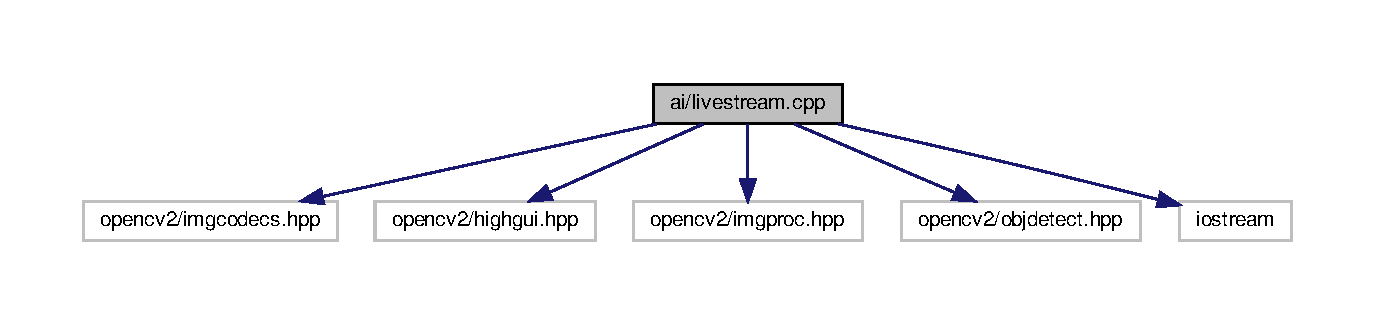
\includegraphics[width=350pt]{livestream_8cpp__incl}
\end{center}
\end{figure}
\subsection*{Functions}
\begin{DoxyCompactItemize}
\item 
int \hyperlink{livestream_8cpp_ae66f6b31b5ad750f1fe042a706a4e3d4}{main} ()
\begin{DoxyCompactList}\small\item\em ///\+Agro\+Pi camera driver for testing a livestream. requires access to raspberry pi gui; cannot be done over V\+Scode S\+SH \end{DoxyCompactList}\end{DoxyCompactItemize}


\subsection{Function Documentation}
\mbox{\Hypertarget{livestream_8cpp_ae66f6b31b5ad750f1fe042a706a4e3d4}\label{livestream_8cpp_ae66f6b31b5ad750f1fe042a706a4e3d4}} 
\index{livestream.\+cpp@{livestream.\+cpp}!main@{main}}
\index{main@{main}!livestream.\+cpp@{livestream.\+cpp}}
\subsubsection{\texorpdfstring{main()}{main()}}
{\footnotesize\ttfamily int main (\begin{DoxyParamCaption}{ }\end{DoxyParamCaption})}



///\+Agro\+Pi camera driver for testing a livestream. requires access to raspberry pi gui; cannot be done over V\+Scode S\+SH 


\hypertarget{ai_2main_8cpp}{}\section{ai/main.cpp File Reference}
\label{ai_2main_8cpp}\index{ai/main.\+cpp@{ai/main.\+cpp}}
{\ttfamily \#include $<$opencv2/opencv.\+hpp$>$}\newline
{\ttfamily \#include $<$opencv2/imgcodecs.\+hpp$>$}\newline
{\ttfamily \#include $<$opencv2/imgproc.\+hpp$>$}\newline
{\ttfamily \#include $<$opencv2/highgui.\+hpp$>$}\newline
{\ttfamily \#include $<$iostream$>$}\newline
Include dependency graph for main.\+cpp\+:\nopagebreak
\begin{figure}[H]
\begin{center}
\leavevmode
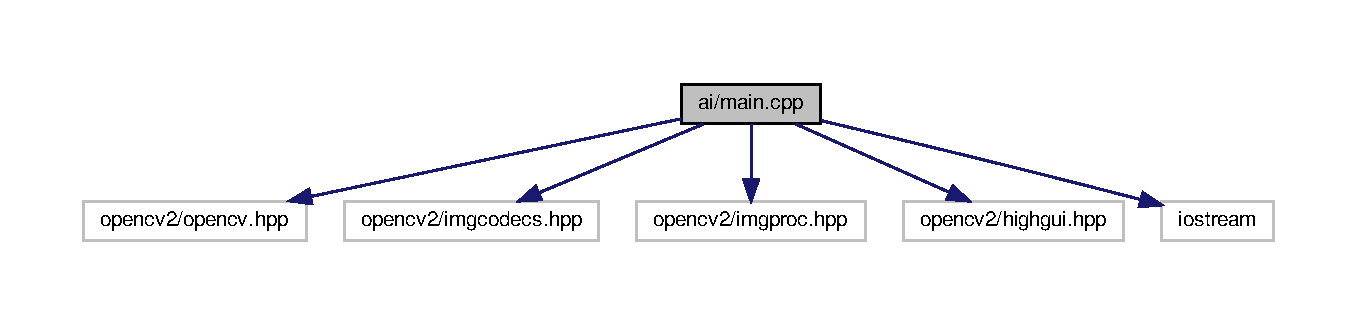
\includegraphics[width=350pt]{ai_2main_8cpp__incl}
\end{center}
\end{figure}
\subsection*{Functions}
\begin{DoxyCompactItemize}
\item 
int \hyperlink{ai_2main_8cpp_ae66f6b31b5ad750f1fe042a706a4e3d4}{main} ()
\end{DoxyCompactItemize}
\subsection*{Variables}
\begin{DoxyCompactItemize}
\item 
cv\+::\+Mat \hyperlink{ai_2main_8cpp_a6dc9e145eafd30060f68789be59f34b7}{img}
\begin{DoxyCompactList}\small\item\em ///\+Agro\+Pi camera driver for taking a picture \end{DoxyCompactList}\item 
cv\+::\+Mat \hyperlink{ai_2main_8cpp_ac4645498726ea4e8a949b4ef1e9de906}{B\+GR}
\item 
cv\+::\+Mat \hyperlink{ai_2main_8cpp_a56ea3886b7236ea8b29e7faa14fa600b}{Norm}
\item 
int \hyperlink{ai_2main_8cpp_a496d35384de8e47c14dbd9cc0e6d3e2d}{cont\+Min} = 0
\item 
int \hyperlink{ai_2main_8cpp_ab8681fd6bf02009826c7900db6e9dca1}{cont\+Max} = 300
\item 
int \hyperlink{ai_2main_8cpp_a23a221013ece5cf46d769d9545bc2f71}{Shut} = 30
\end{DoxyCompactItemize}


\subsection{Function Documentation}
\mbox{\Hypertarget{ai_2main_8cpp_ae66f6b31b5ad750f1fe042a706a4e3d4}\label{ai_2main_8cpp_ae66f6b31b5ad750f1fe042a706a4e3d4}} 
\index{ai/main.\+cpp@{ai/main.\+cpp}!main@{main}}
\index{main@{main}!ai/main.\+cpp@{ai/main.\+cpp}}
\subsubsection{\texorpdfstring{main()}{main()}}
{\footnotesize\ttfamily int main (\begin{DoxyParamCaption}{ }\end{DoxyParamCaption})}



\subsection{Variable Documentation}
\mbox{\Hypertarget{ai_2main_8cpp_ac4645498726ea4e8a949b4ef1e9de906}\label{ai_2main_8cpp_ac4645498726ea4e8a949b4ef1e9de906}} 
\index{ai/main.\+cpp@{ai/main.\+cpp}!B\+GR@{B\+GR}}
\index{B\+GR@{B\+GR}!ai/main.\+cpp@{ai/main.\+cpp}}
\subsubsection{\texorpdfstring{B\+GR}{BGR}}
{\footnotesize\ttfamily cv\+::\+Mat B\+GR}

\mbox{\Hypertarget{ai_2main_8cpp_ab8681fd6bf02009826c7900db6e9dca1}\label{ai_2main_8cpp_ab8681fd6bf02009826c7900db6e9dca1}} 
\index{ai/main.\+cpp@{ai/main.\+cpp}!cont\+Max@{cont\+Max}}
\index{cont\+Max@{cont\+Max}!ai/main.\+cpp@{ai/main.\+cpp}}
\subsubsection{\texorpdfstring{cont\+Max}{contMax}}
{\footnotesize\ttfamily int cont\+Max = 300}

\mbox{\Hypertarget{ai_2main_8cpp_a496d35384de8e47c14dbd9cc0e6d3e2d}\label{ai_2main_8cpp_a496d35384de8e47c14dbd9cc0e6d3e2d}} 
\index{ai/main.\+cpp@{ai/main.\+cpp}!cont\+Min@{cont\+Min}}
\index{cont\+Min@{cont\+Min}!ai/main.\+cpp@{ai/main.\+cpp}}
\subsubsection{\texorpdfstring{cont\+Min}{contMin}}
{\footnotesize\ttfamily int cont\+Min = 0}

\mbox{\Hypertarget{ai_2main_8cpp_a6dc9e145eafd30060f68789be59f34b7}\label{ai_2main_8cpp_a6dc9e145eafd30060f68789be59f34b7}} 
\index{ai/main.\+cpp@{ai/main.\+cpp}!img@{img}}
\index{img@{img}!ai/main.\+cpp@{ai/main.\+cpp}}
\subsubsection{\texorpdfstring{img}{img}}
{\footnotesize\ttfamily cv\+::\+Mat img}



///\+Agro\+Pi camera driver for taking a picture 

\mbox{\Hypertarget{ai_2main_8cpp_a56ea3886b7236ea8b29e7faa14fa600b}\label{ai_2main_8cpp_a56ea3886b7236ea8b29e7faa14fa600b}} 
\index{ai/main.\+cpp@{ai/main.\+cpp}!Norm@{Norm}}
\index{Norm@{Norm}!ai/main.\+cpp@{ai/main.\+cpp}}
\subsubsection{\texorpdfstring{Norm}{Norm}}
{\footnotesize\ttfamily cv\+::\+Mat Norm}

\mbox{\Hypertarget{ai_2main_8cpp_a23a221013ece5cf46d769d9545bc2f71}\label{ai_2main_8cpp_a23a221013ece5cf46d769d9545bc2f71}} 
\index{ai/main.\+cpp@{ai/main.\+cpp}!Shut@{Shut}}
\index{Shut@{Shut}!ai/main.\+cpp@{ai/main.\+cpp}}
\subsubsection{\texorpdfstring{Shut}{Shut}}
{\footnotesize\ttfamily int Shut = 30}


\hypertarget{src_2main_8cpp}{}\section{src/main.cpp File Reference}
\label{src_2main_8cpp}\index{src/main.\+cpp@{src/main.\+cpp}}
{\ttfamily \#include \char`\"{}Controller\+Thread.\+h\char`\"{}}\newline
Include dependency graph for main.\+cpp\+:\nopagebreak
\begin{figure}[H]
\begin{center}
\leavevmode
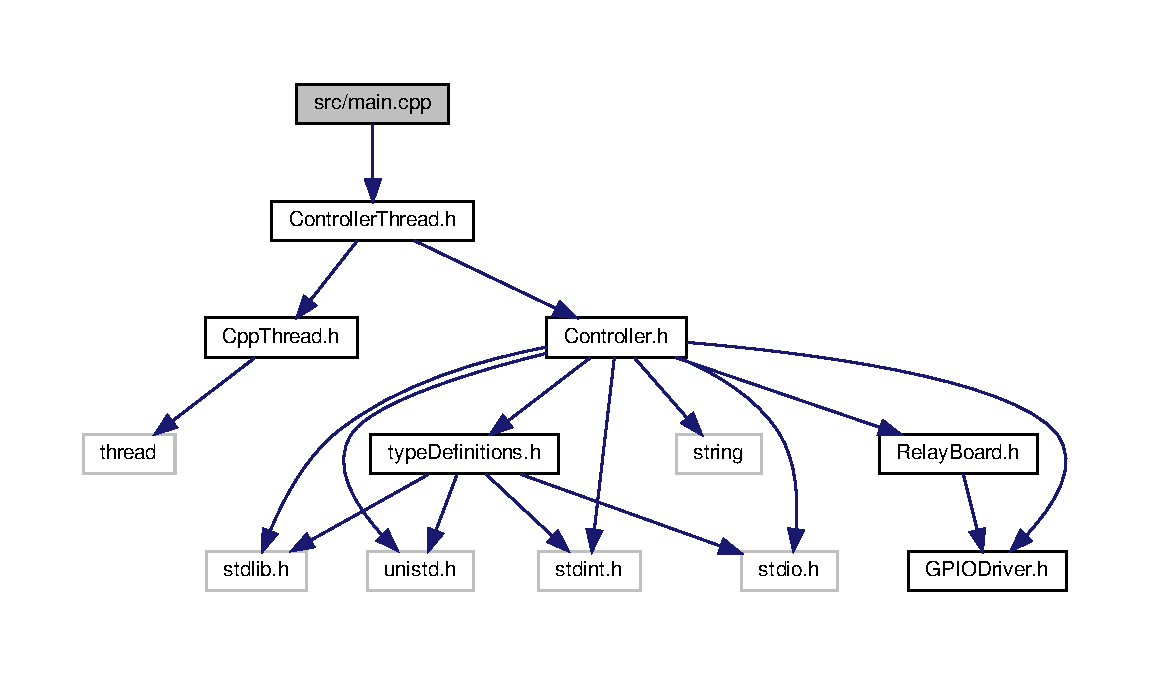
\includegraphics[width=350pt]{src_2main_8cpp__incl}
\end{center}
\end{figure}
\subsection*{Functions}
\begin{DoxyCompactItemize}
\item 
int \hyperlink{src_2main_8cpp_ac0f2228420376f4db7e1274f2b41667c}{main} (int argc, const char $\ast$argv\mbox{[}$\,$\mbox{]})
\end{DoxyCompactItemize}


\subsection{Function Documentation}
\mbox{\Hypertarget{src_2main_8cpp_ac0f2228420376f4db7e1274f2b41667c}\label{src_2main_8cpp_ac0f2228420376f4db7e1274f2b41667c}} 
\index{src/main.\+cpp@{src/main.\+cpp}!main@{main}}
\index{main@{main}!src/main.\+cpp@{src/main.\+cpp}}
\subsubsection{\texorpdfstring{main()}{main()}}
{\footnotesize\ttfamily int main (\begin{DoxyParamCaption}\item[{int}]{argc,  }\item[{const char $\ast$}]{argv\mbox{[}$\,$\mbox{]} }\end{DoxyParamCaption})}


\hypertarget{CONTRIBUTING_8md}{}\section{docs/\+C\+O\+N\+T\+R\+I\+B\+U\+T\+I\+NG.md File Reference}
\label{CONTRIBUTING_8md}\index{docs/\+C\+O\+N\+T\+R\+I\+B\+U\+T\+I\+N\+G.\+md@{docs/\+C\+O\+N\+T\+R\+I\+B\+U\+T\+I\+N\+G.\+md}}

\hypertarget{Design_8md}{}\section{docs/\+Design.md File Reference}
\label{Design_8md}\index{docs/\+Design.\+md@{docs/\+Design.\+md}}

\hypertarget{FileFolderStructure_8md}{}\section{docs/\+File\+Folder\+Structure.md File Reference}
\label{FileFolderStructure_8md}\index{docs/\+File\+Folder\+Structure.\+md@{docs/\+File\+Folder\+Structure.\+md}}

\hypertarget{roadmap_8md}{}\section{docs/roadmap.md File Reference}
\label{roadmap_8md}\index{docs/roadmap.\+md@{docs/roadmap.\+md}}

\hypertarget{Controller_8cpp}{}\section{src/controller/\+Controller.cpp File Reference}
\label{Controller_8cpp}\index{src/controller/\+Controller.\+cpp@{src/controller/\+Controller.\+cpp}}
{\ttfamily \#include \char`\"{}Controller.\+h\char`\"{}}\newline
{\ttfamily \#include $<$stdio.\+h$>$}\newline
{\ttfamily \#include $<$string$>$}\newline
{\ttfamily \#include $<$iostream$>$}\newline
{\ttfamily \#include \char`\"{}httplib.\+h\char`\"{}}\newline
Include dependency graph for Controller.\+cpp\+:\nopagebreak
\begin{figure}[H]
\begin{center}
\leavevmode
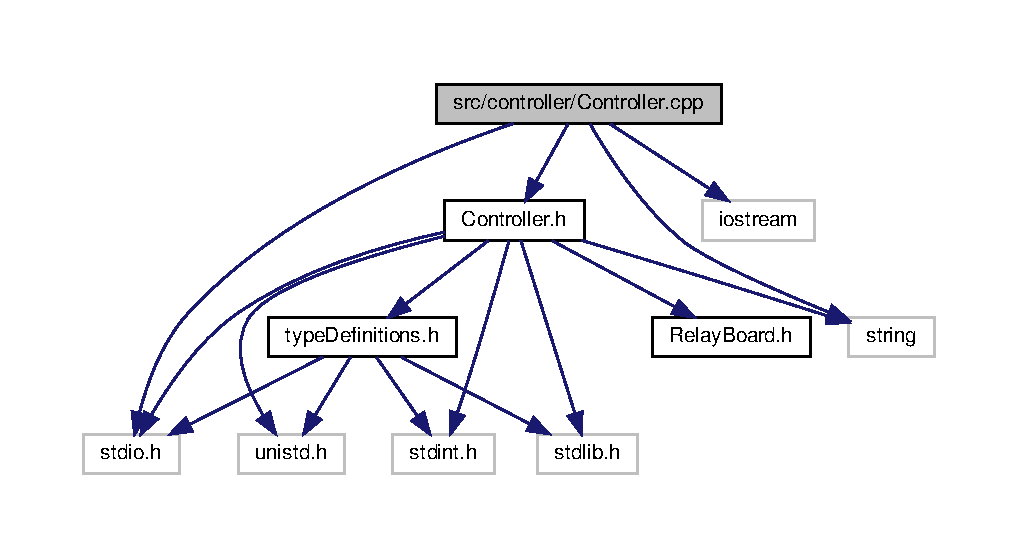
\includegraphics[width=350pt]{Controller_8cpp__incl}
\end{center}
\end{figure}
\subsection*{Macros}
\begin{DoxyCompactItemize}
\item 
\#define \hyperlink{Controller_8cpp_a261c321c196e81758a042f0ae37aca7f}{C\+P\+P\+H\+T\+T\+P\+L\+I\+B\+\_\+\+O\+P\+E\+N\+S\+S\+L\+\_\+\+S\+U\+P\+P\+O\+RT}
\end{DoxyCompactItemize}


\subsection{Detailed Description}
\begin{DoxyAuthor}{Author}
Kamil Rog 
\end{DoxyAuthor}
\begin{DoxyVersion}{Version}
0.\+1
\end{DoxyVersion}
This file contains the functions for actuator class. 

\subsection{Macro Definition Documentation}
\mbox{\Hypertarget{Controller_8cpp_a261c321c196e81758a042f0ae37aca7f}\label{Controller_8cpp_a261c321c196e81758a042f0ae37aca7f}} 
\index{Controller.\+cpp@{Controller.\+cpp}!C\+P\+P\+H\+T\+T\+P\+L\+I\+B\+\_\+\+O\+P\+E\+N\+S\+S\+L\+\_\+\+S\+U\+P\+P\+O\+RT@{C\+P\+P\+H\+T\+T\+P\+L\+I\+B\+\_\+\+O\+P\+E\+N\+S\+S\+L\+\_\+\+S\+U\+P\+P\+O\+RT}}
\index{C\+P\+P\+H\+T\+T\+P\+L\+I\+B\+\_\+\+O\+P\+E\+N\+S\+S\+L\+\_\+\+S\+U\+P\+P\+O\+RT@{C\+P\+P\+H\+T\+T\+P\+L\+I\+B\+\_\+\+O\+P\+E\+N\+S\+S\+L\+\_\+\+S\+U\+P\+P\+O\+RT}!Controller.\+cpp@{Controller.\+cpp}}
\subsubsection{\texorpdfstring{C\+P\+P\+H\+T\+T\+P\+L\+I\+B\+\_\+\+O\+P\+E\+N\+S\+S\+L\+\_\+\+S\+U\+P\+P\+O\+RT}{CPPHTTPLIB\_OPENSSL\_SUPPORT}}
{\footnotesize\ttfamily \#define C\+P\+P\+H\+T\+T\+P\+L\+I\+B\+\_\+\+O\+P\+E\+N\+S\+S\+L\+\_\+\+S\+U\+P\+P\+O\+RT}


\hypertarget{Controller_8h}{}\section{src/controller/\+Controller.h File Reference}
\label{Controller_8h}\index{src/controller/\+Controller.\+h@{src/controller/\+Controller.\+h}}
{\ttfamily \#include \char`\"{}type\+Definitions.\+h\char`\"{}}\newline
{\ttfamily \#include \char`\"{}Relay\+Board.\+h\char`\"{}}\newline
{\ttfamily \#include $<$string$>$}\newline
Include dependency graph for Controller.\+h\+:\nopagebreak
\begin{figure}[H]
\begin{center}
\leavevmode
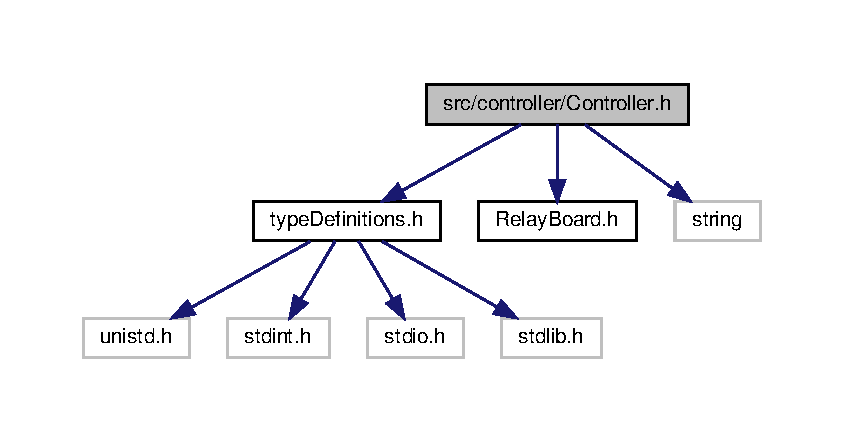
\includegraphics[width=350pt]{Controller_8h__incl}
\end{center}
\end{figure}
This graph shows which files directly or indirectly include this file\+:\nopagebreak
\begin{figure}[H]
\begin{center}
\leavevmode
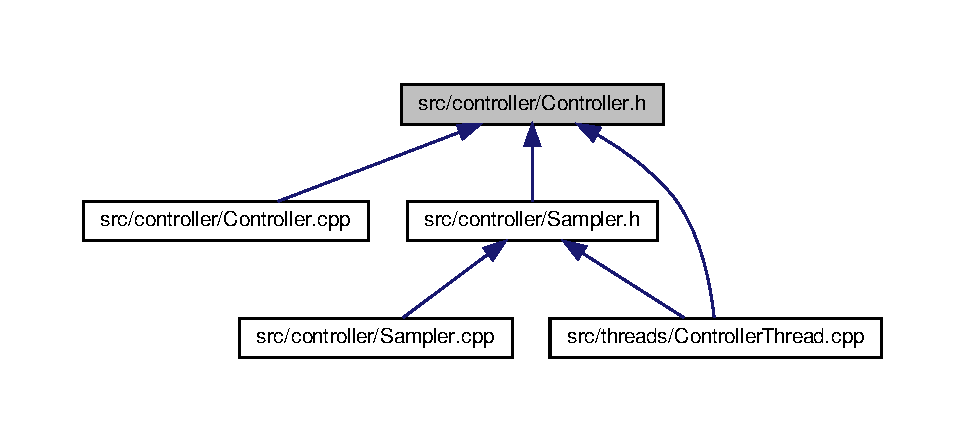
\includegraphics[width=350pt]{Controller_8h__dep__incl}
\end{center}
\end{figure}
\subsection*{Classes}
\begin{DoxyCompactItemize}
\item 
class \hyperlink{classController}{Controller}
\begin{DoxyCompactList}\small\item\em \hyperlink{classController}{Controller} class. \end{DoxyCompactList}\end{DoxyCompactItemize}


\subsection{Detailed Description}
\begin{DoxyAuthor}{Author}
Kamil Rog 
\end{DoxyAuthor}
\begin{DoxyVersion}{Version}
0.\+1
\end{DoxyVersion}
\hypertarget{Controller.h_DESCRIPTION}{}\subsection{D\+E\+S\+C\+R\+I\+P\+T\+I\+ON}\label{Controller.h_DESCRIPTION}

\hypertarget{Camera_8cpp}{}\section{src/controller/peripherials/\+Camera.cpp File Reference}
\label{Camera_8cpp}\index{src/controller/peripherials/\+Camera.\+cpp@{src/controller/peripherials/\+Camera.\+cpp}}
{\ttfamily \#include \char`\"{}Camera.\+h\char`\"{}}\newline
{\ttfamily \#include $<$ctime$>$}\newline
{\ttfamily \#include $<$iostream$>$}\newline
Include dependency graph for Camera.\+cpp\+:\nopagebreak
\begin{figure}[H]
\begin{center}
\leavevmode
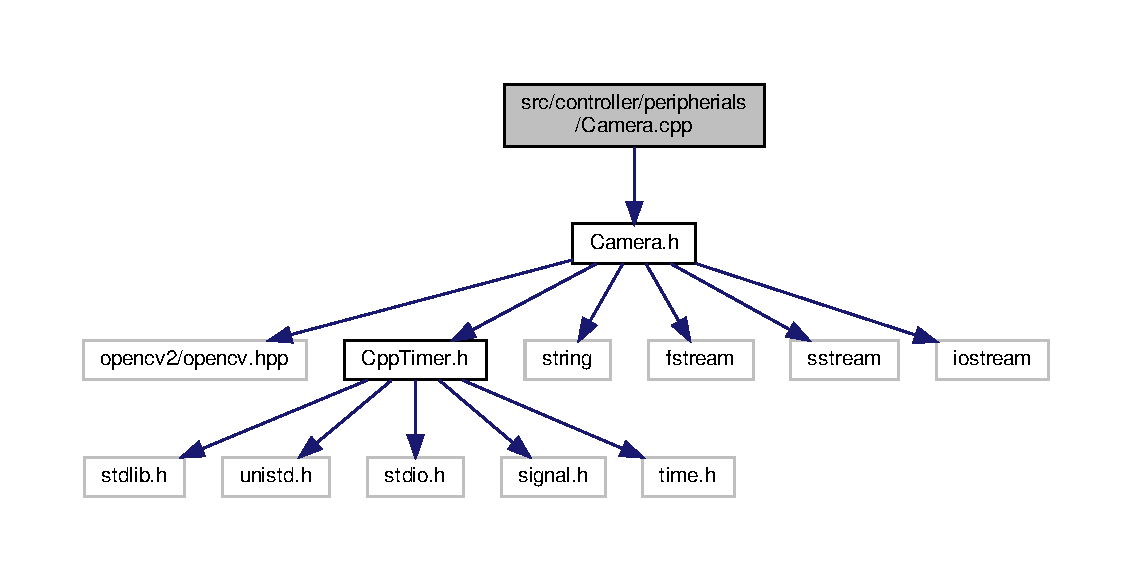
\includegraphics[width=271pt]{Camera_8cpp__incl}
\end{center}
\end{figure}


\subsection{Detailed Description}
\begin{DoxyAuthor}{Author}
Kamil Rog 
\end{DoxyAuthor}
\begin{DoxyVersion}{Version}
0.\+1
\end{DoxyVersion}
This file contains the functions for R\+Pi \hyperlink{classCamera}{Camera} class. 
\hypertarget{Camera_8h}{}\section{src/controller/peripherials/\+Camera.h File Reference}
\label{Camera_8h}\index{src/controller/peripherials/\+Camera.\+h@{src/controller/peripherials/\+Camera.\+h}}
This graph shows which files directly or indirectly include this file\+:\nopagebreak
\begin{figure}[H]
\begin{center}
\leavevmode
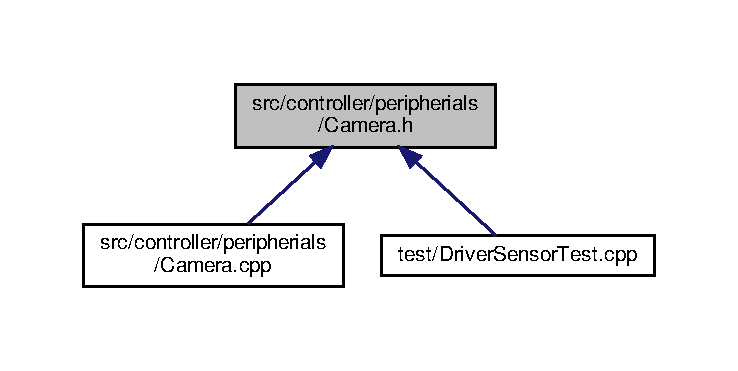
\includegraphics[width=350pt]{Camera_8h__dep__incl}
\end{center}
\end{figure}
\subsection*{Classes}
\begin{DoxyCompactItemize}
\item 
class \hyperlink{classCamera}{Camera}
\begin{DoxyCompactList}\small\item\em \hyperlink{classCamera}{Camera} class. \end{DoxyCompactList}\end{DoxyCompactItemize}


\subsection{Detailed Description}
\begin{DoxyAuthor}{Author}
Kamil Rog 
\end{DoxyAuthor}
\begin{DoxyVersion}{Version}
0.\+1
\end{DoxyVersion}
This header file contains the class for the R\+Pi \hyperlink{classCamera}{Camera}. 
\hypertarget{I2CDriver_8cpp}{}\section{src/controller/peripherials/\+I2\+C\+Driver.cpp File Reference}
\label{I2CDriver_8cpp}\index{src/controller/peripherials/\+I2\+C\+Driver.\+cpp@{src/controller/peripherials/\+I2\+C\+Driver.\+cpp}}
{\ttfamily \#include \char`\"{}I2\+C\+Driver.\+h\char`\"{}}\newline
{\ttfamily \#include $<$stdio.\+h$>$}\newline
{\ttfamily \#include $<$unistd.\+h$>$}\newline
{\ttfamily \#include $<$time.\+h$>$}\newline
{\ttfamily \#include $<$fcntl.\+h$>$}\newline
{\ttfamily \#include $<$sys/ioctl.\+h$>$}\newline
{\ttfamily \#include $<$errno.\+h$>$}\newline
{\ttfamily \#include $<$string.\+h$>$}\newline
{\ttfamily \#include \char`\"{}i2c/smbus.\+h\char`\"{}}\newline
{\ttfamily \#include $<$linux/i2c-\/dev.\+h$>$}\newline
{\ttfamily \#include $<$linux/i2c.\+h$>$}\newline
{\ttfamily \#include \char`\"{}utils.\+h\char`\"{}}\newline
Include dependency graph for I2\+C\+Driver.\+cpp\+:\nopagebreak
\begin{figure}[H]
\begin{center}
\leavevmode
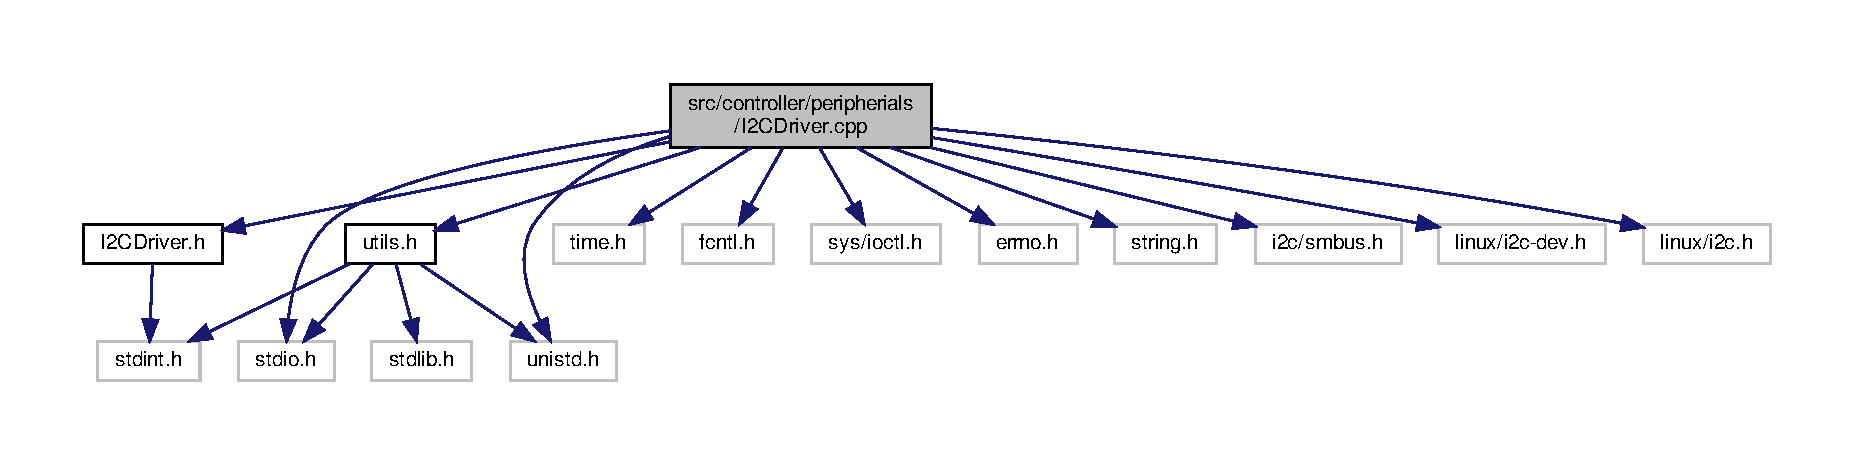
\includegraphics[width=350pt]{I2CDriver_8cpp__incl}
\end{center}
\end{figure}
\subsection*{Macros}
\begin{DoxyCompactItemize}
\item 
\#define \hyperlink{I2CDriver_8cpp_a2694a39dfd1fa087ca6f9f391c91dae7}{C\+L\+O\+C\+K\+ID}~C\+L\+O\+C\+K\+\_\+\+M\+O\+N\+O\+T\+O\+N\+IC
\end{DoxyCompactItemize}


\subsection{Detailed Description}
\begin{DoxyAuthor}{Author}
Andrew Scott-\/\+George 
\end{DoxyAuthor}
\begin{DoxyVersion}{Version}
0.\+1
\end{DoxyVersion}
This file contains the functions for \hyperlink{classCamera}{Camera} class. It acts as a wrapper for Open\+CV functions, contextualising them in a \hyperlink{classCamera}{Camera} class.

\href{https://opencv.org/}{\tt https\+://opencv.\+org/}

\begin{DoxyAuthor}{Author}
Andrew Scott-\/\+George \& Kamil Rog 
\end{DoxyAuthor}
\begin{DoxyVersion}{Version}
0.\+1
\end{DoxyVersion}
This file contains the class for the \hyperlink{classCamera}{Camera} driver

\begin{DoxyAuthor}{Author}
Kamil Rog 
\end{DoxyAuthor}
\begin{DoxyVersion}{Version}
0.\+1
\end{DoxyVersion}
This file contains the functions for I2C Driver Class. Essentially this is a wrapper for the A\+PI provided for I2C Linux Driver. Conatins functions for plain I2C and S\+M\+B\+US

\href{https://www.kernel.org/doc/html/latest/driver-api/i2c}{\tt https\+://www.\+kernel.\+org/doc/html/latest/driver-\/api/i2c}. \href{https://www.i2c-bus.org/smbus/}{\tt https\+://www.\+i2c-\/bus.\+org/smbus/} 

\subsection{Macro Definition Documentation}
\mbox{\Hypertarget{I2CDriver_8cpp_a2694a39dfd1fa087ca6f9f391c91dae7}\label{I2CDriver_8cpp_a2694a39dfd1fa087ca6f9f391c91dae7}} 
\index{I2\+C\+Driver.\+cpp@{I2\+C\+Driver.\+cpp}!C\+L\+O\+C\+K\+ID@{C\+L\+O\+C\+K\+ID}}
\index{C\+L\+O\+C\+K\+ID@{C\+L\+O\+C\+K\+ID}!I2\+C\+Driver.\+cpp@{I2\+C\+Driver.\+cpp}}
\subsubsection{\texorpdfstring{C\+L\+O\+C\+K\+ID}{CLOCKID}}
{\footnotesize\ttfamily \#define C\+L\+O\+C\+K\+ID~C\+L\+O\+C\+K\+\_\+\+M\+O\+N\+O\+T\+O\+N\+IC}


\hypertarget{I2CDriver_8h}{}\section{src/controller/peripherials/\+I2\+C\+Driver.h File Reference}
\label{I2CDriver_8h}\index{src/controller/peripherials/\+I2\+C\+Driver.\+h@{src/controller/peripherials/\+I2\+C\+Driver.\+h}}
{\ttfamily \#include $<$stdint.\+h$>$}\newline
Include dependency graph for I2\+C\+Driver.\+h\+:\nopagebreak
\begin{figure}[H]
\begin{center}
\leavevmode
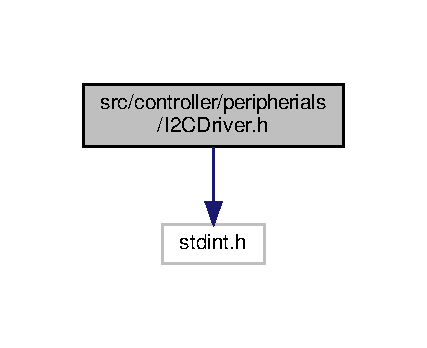
\includegraphics[width=205pt]{I2CDriver_8h__incl}
\end{center}
\end{figure}
This graph shows which files directly or indirectly include this file\+:\nopagebreak
\begin{figure}[H]
\begin{center}
\leavevmode
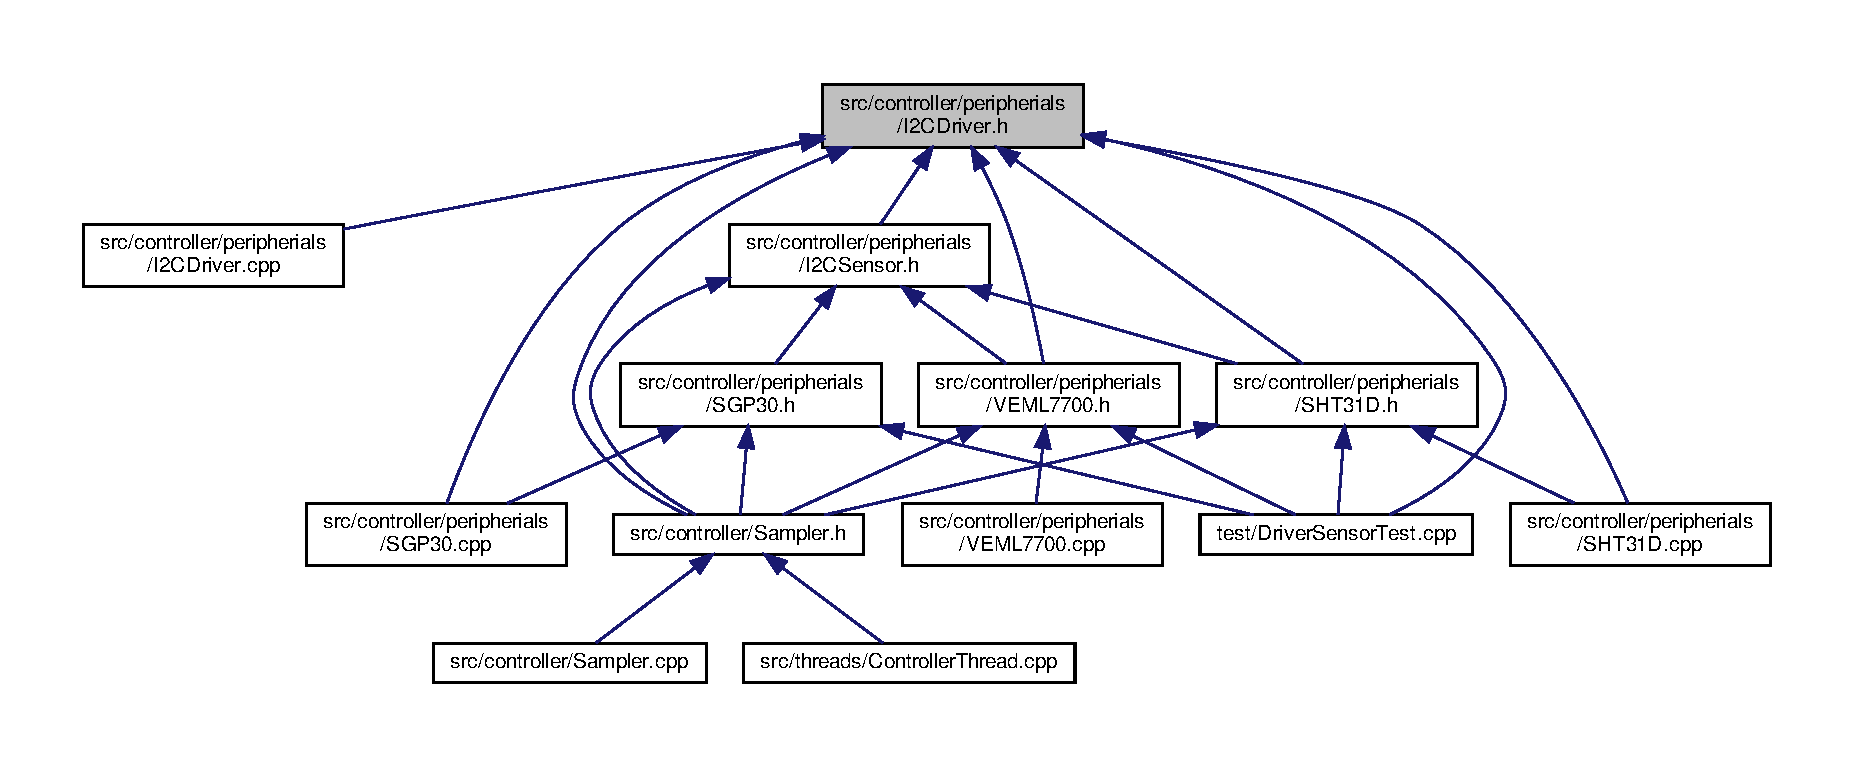
\includegraphics[width=350pt]{I2CDriver_8h__dep__incl}
\end{center}
\end{figure}
\subsection*{Classes}
\begin{DoxyCompactItemize}
\item 
class \hyperlink{classI2CDriver}{I2\+C\+Driver}
\begin{DoxyCompactList}\small\item\em I2C Driver class. \end{DoxyCompactList}\end{DoxyCompactItemize}
\subsection*{Enumerations}
\begin{DoxyCompactItemize}
\item 
enum \hyperlink{I2CDriver_8h_a52c38e7692a76e897b00daa867b29d3f}{I2\+C\+\_\+\+Return} \{ \newline
\hyperlink{I2CDriver_8h_a52c38e7692a76e897b00daa867b29d3faeceba296bdda2b90e8835c431fe7a72a}{I2\+C\+\_\+\+OK} = 0, 
\hyperlink{I2CDriver_8h_a52c38e7692a76e897b00daa867b29d3faa978b8c99ba81b70dcb4a660ec190c8b}{I2\+C\+\_\+\+I\+O\+C\+T\+L\+\_\+\+F\+A\+I\+L\+ED} = -\/1, 
\hyperlink{I2CDriver_8h_a52c38e7692a76e897b00daa867b29d3fa43b4aeb860553fe1c22ab94cb6b4a446}{I2\+C\+\_\+\+W\+R\+I\+T\+E\+\_\+\+F\+A\+I\+L\+ED} = -\/2, 
\hyperlink{I2CDriver_8h_a52c38e7692a76e897b00daa867b29d3fac86dfc8232f86c65e33a1b9491763a21}{I2\+C\+\_\+\+R\+E\+A\+D\+\_\+\+F\+A\+I\+L\+ED} = -\/3, 
\newline
\hyperlink{I2CDriver_8h_a52c38e7692a76e897b00daa867b29d3fa63b31d0c504bdae545fb5da13d59c986}{I2\+C\+\_\+\+C\+R\+C\+\_\+\+F\+A\+I\+L\+ED} = -\/4, 
\hyperlink{I2CDriver_8h_a52c38e7692a76e897b00daa867b29d3fa2fa4d728abcc354ab37d4ff073289900}{I2\+C\+\_\+\+F\+A\+IL} = -\/5
 \}
\end{DoxyCompactItemize}


\subsection{Detailed Description}
\begin{DoxyAuthor}{Author}
Kamil Rog 
\end{DoxyAuthor}
\begin{DoxyVersion}{Version}
0.\+1
\end{DoxyVersion}
This file contains the class for the I2C Driver 

\subsection{Enumeration Type Documentation}
\mbox{\Hypertarget{I2CDriver_8h_a52c38e7692a76e897b00daa867b29d3f}\label{I2CDriver_8h_a52c38e7692a76e897b00daa867b29d3f}} 
\index{I2\+C\+Driver.\+h@{I2\+C\+Driver.\+h}!I2\+C\+\_\+\+Return@{I2\+C\+\_\+\+Return}}
\index{I2\+C\+\_\+\+Return@{I2\+C\+\_\+\+Return}!I2\+C\+Driver.\+h@{I2\+C\+Driver.\+h}}
\subsubsection{\texorpdfstring{I2\+C\+\_\+\+Return}{I2C\_Return}}
{\footnotesize\ttfamily enum \hyperlink{I2CDriver_8h_a52c38e7692a76e897b00daa867b29d3f}{I2\+C\+\_\+\+Return}}

Return Status Enumeration \begin{DoxyEnumFields}{Enumerator}
\raisebox{\heightof{T}}[0pt][0pt]{\index{I2\+C\+\_\+\+OK@{I2\+C\+\_\+\+OK}!I2\+C\+Driver.\+h@{I2\+C\+Driver.\+h}}\index{I2\+C\+Driver.\+h@{I2\+C\+Driver.\+h}!I2\+C\+\_\+\+OK@{I2\+C\+\_\+\+OK}}}\mbox{\Hypertarget{I2CDriver_8h_a52c38e7692a76e897b00daa867b29d3faeceba296bdda2b90e8835c431fe7a72a}\label{I2CDriver_8h_a52c38e7692a76e897b00daa867b29d3faeceba296bdda2b90e8835c431fe7a72a}} 
I2\+C\+\_\+\+OK&\\
\hline

\raisebox{\heightof{T}}[0pt][0pt]{\index{I2\+C\+\_\+\+I\+O\+C\+T\+L\+\_\+\+F\+A\+I\+L\+ED@{I2\+C\+\_\+\+I\+O\+C\+T\+L\+\_\+\+F\+A\+I\+L\+ED}!I2\+C\+Driver.\+h@{I2\+C\+Driver.\+h}}\index{I2\+C\+Driver.\+h@{I2\+C\+Driver.\+h}!I2\+C\+\_\+\+I\+O\+C\+T\+L\+\_\+\+F\+A\+I\+L\+ED@{I2\+C\+\_\+\+I\+O\+C\+T\+L\+\_\+\+F\+A\+I\+L\+ED}}}\mbox{\Hypertarget{I2CDriver_8h_a52c38e7692a76e897b00daa867b29d3faa978b8c99ba81b70dcb4a660ec190c8b}\label{I2CDriver_8h_a52c38e7692a76e897b00daa867b29d3faa978b8c99ba81b70dcb4a660ec190c8b}} 
I2\+C\+\_\+\+I\+O\+C\+T\+L\+\_\+\+F\+A\+I\+L\+ED&\\
\hline

\raisebox{\heightof{T}}[0pt][0pt]{\index{I2\+C\+\_\+\+W\+R\+I\+T\+E\+\_\+\+F\+A\+I\+L\+ED@{I2\+C\+\_\+\+W\+R\+I\+T\+E\+\_\+\+F\+A\+I\+L\+ED}!I2\+C\+Driver.\+h@{I2\+C\+Driver.\+h}}\index{I2\+C\+Driver.\+h@{I2\+C\+Driver.\+h}!I2\+C\+\_\+\+W\+R\+I\+T\+E\+\_\+\+F\+A\+I\+L\+ED@{I2\+C\+\_\+\+W\+R\+I\+T\+E\+\_\+\+F\+A\+I\+L\+ED}}}\mbox{\Hypertarget{I2CDriver_8h_a52c38e7692a76e897b00daa867b29d3fa43b4aeb860553fe1c22ab94cb6b4a446}\label{I2CDriver_8h_a52c38e7692a76e897b00daa867b29d3fa43b4aeb860553fe1c22ab94cb6b4a446}} 
I2\+C\+\_\+\+W\+R\+I\+T\+E\+\_\+\+F\+A\+I\+L\+ED&\\
\hline

\raisebox{\heightof{T}}[0pt][0pt]{\index{I2\+C\+\_\+\+R\+E\+A\+D\+\_\+\+F\+A\+I\+L\+ED@{I2\+C\+\_\+\+R\+E\+A\+D\+\_\+\+F\+A\+I\+L\+ED}!I2\+C\+Driver.\+h@{I2\+C\+Driver.\+h}}\index{I2\+C\+Driver.\+h@{I2\+C\+Driver.\+h}!I2\+C\+\_\+\+R\+E\+A\+D\+\_\+\+F\+A\+I\+L\+ED@{I2\+C\+\_\+\+R\+E\+A\+D\+\_\+\+F\+A\+I\+L\+ED}}}\mbox{\Hypertarget{I2CDriver_8h_a52c38e7692a76e897b00daa867b29d3fac86dfc8232f86c65e33a1b9491763a21}\label{I2CDriver_8h_a52c38e7692a76e897b00daa867b29d3fac86dfc8232f86c65e33a1b9491763a21}} 
I2\+C\+\_\+\+R\+E\+A\+D\+\_\+\+F\+A\+I\+L\+ED&\\
\hline

\raisebox{\heightof{T}}[0pt][0pt]{\index{I2\+C\+\_\+\+C\+R\+C\+\_\+\+F\+A\+I\+L\+ED@{I2\+C\+\_\+\+C\+R\+C\+\_\+\+F\+A\+I\+L\+ED}!I2\+C\+Driver.\+h@{I2\+C\+Driver.\+h}}\index{I2\+C\+Driver.\+h@{I2\+C\+Driver.\+h}!I2\+C\+\_\+\+C\+R\+C\+\_\+\+F\+A\+I\+L\+ED@{I2\+C\+\_\+\+C\+R\+C\+\_\+\+F\+A\+I\+L\+ED}}}\mbox{\Hypertarget{I2CDriver_8h_a52c38e7692a76e897b00daa867b29d3fa63b31d0c504bdae545fb5da13d59c986}\label{I2CDriver_8h_a52c38e7692a76e897b00daa867b29d3fa63b31d0c504bdae545fb5da13d59c986}} 
I2\+C\+\_\+\+C\+R\+C\+\_\+\+F\+A\+I\+L\+ED&\\
\hline

\raisebox{\heightof{T}}[0pt][0pt]{\index{I2\+C\+\_\+\+F\+A\+IL@{I2\+C\+\_\+\+F\+A\+IL}!I2\+C\+Driver.\+h@{I2\+C\+Driver.\+h}}\index{I2\+C\+Driver.\+h@{I2\+C\+Driver.\+h}!I2\+C\+\_\+\+F\+A\+IL@{I2\+C\+\_\+\+F\+A\+IL}}}\mbox{\Hypertarget{I2CDriver_8h_a52c38e7692a76e897b00daa867b29d3fa2fa4d728abcc354ab37d4ff073289900}\label{I2CDriver_8h_a52c38e7692a76e897b00daa867b29d3fa2fa4d728abcc354ab37d4ff073289900}} 
I2\+C\+\_\+\+F\+A\+IL&\\
\hline

\end{DoxyEnumFields}

\hypertarget{I2CSensor_8h}{}\section{src/controller/peripherials/\+I2\+C\+Sensor.h File Reference}
\label{I2CSensor_8h}\index{src/controller/peripherials/\+I2\+C\+Sensor.\+h@{src/controller/peripherials/\+I2\+C\+Sensor.\+h}}
{\ttfamily \#include $<$stdlib.\+h$>$}\newline
{\ttfamily \#include $<$unistd.\+h$>$}\newline
{\ttfamily \#include $<$stdio.\+h$>$}\newline
{\ttfamily \#include \char`\"{}I2\+C\+Driver.\+h\char`\"{}}\newline
Include dependency graph for I2\+C\+Sensor.\+h\+:\nopagebreak
\begin{figure}[H]
\begin{center}
\leavevmode
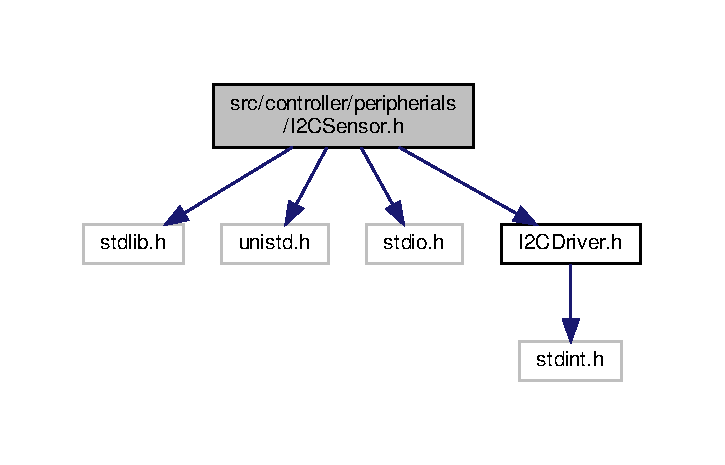
\includegraphics[width=348pt]{I2CSensor_8h__incl}
\end{center}
\end{figure}
This graph shows which files directly or indirectly include this file\+:\nopagebreak
\begin{figure}[H]
\begin{center}
\leavevmode
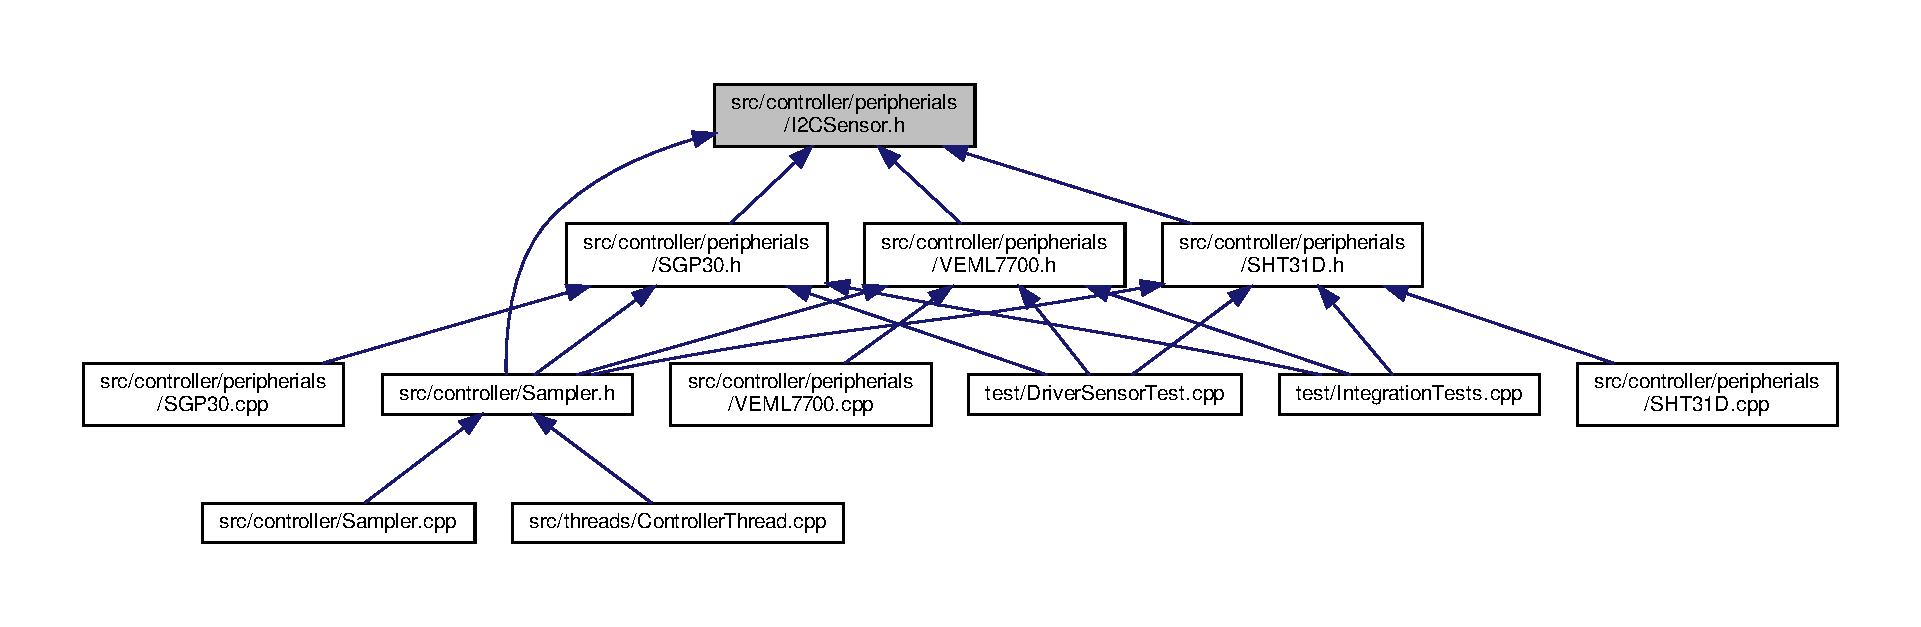
\includegraphics[width=350pt]{I2CSensor_8h__dep__incl}
\end{center}
\end{figure}
\subsection*{Classes}
\begin{DoxyCompactItemize}
\item 
class \hyperlink{classI2CSensor}{I2\+C\+Sensor}
\end{DoxyCompactItemize}

\hypertarget{RelayBoard_8cpp}{}\section{src/controller/peripherials/\+Relay\+Board.cpp File Reference}
\label{RelayBoard_8cpp}\index{src/controller/peripherials/\+Relay\+Board.\+cpp@{src/controller/peripherials/\+Relay\+Board.\+cpp}}
{\ttfamily \#include \char`\"{}Relay\+Board.\+h\char`\"{}}\newline
{\ttfamily \#include $<$errno.\+h$>$}\newline
{\ttfamily \#include $<$fcntl.\+h$>$}\newline
{\ttfamily \#include $<$stdio.\+h$>$}\newline
{\ttfamily \#include $<$stdlib.\+h$>$}\newline
{\ttfamily \#include $<$sys/stat.\+h$>$}\newline
{\ttfamily \#include $<$sys/types.\+h$>$}\newline
{\ttfamily \#include $<$unistd.\+h$>$}\newline
{\ttfamily \#include $<$string$>$}\newline
{\ttfamily \#include $<$iostream$>$}\newline
{\ttfamily \#include $<$sys/mman.\+h$>$}\newline
Include dependency graph for Relay\+Board.\+cpp\+:\nopagebreak
\begin{figure}[H]
\begin{center}
\leavevmode
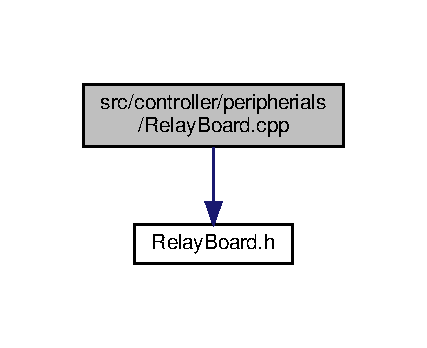
\includegraphics[width=350pt]{RelayBoard_8cpp__incl}
\end{center}
\end{figure}
\subsection*{Macros}
\begin{DoxyCompactItemize}
\item 
\#define \hyperlink{RelayBoard_8cpp_ac2bbd6d630a06a980d9a92ddb9a49928}{IN}~0
\item 
\#define \hyperlink{RelayBoard_8cpp_aec78e7a9e90a406a56f859ee456e8eae}{O\+UT}~1
\item 
\#define \hyperlink{RelayBoard_8cpp_ab811d8c6ff3a505312d3276590444289}{L\+OW}~0
\item 
\#define \hyperlink{RelayBoard_8cpp_a5bb885982ff66a2e0a0a45a8ee9c35e2}{H\+I\+GH}~1
\item 
\#define \hyperlink{RelayBoard_8cpp_a6b20d41d6252e9871430c242cb1a56e7}{B\+U\+F\+F\+E\+R\+\_\+\+S\+I\+ZE}~3
\item 
\#define \hyperlink{RelayBoard_8cpp_aa65936c8accb6e3766be6ee9f063ead4}{D\+I\+R\+E\+C\+T\+I\+O\+N\+\_\+\+M\+AX}~35
\item 
\#define \hyperlink{RelayBoard_8cpp_aacdeb883b8cfc24b1ea6133e987a556d}{V\+A\+L\+U\+E\+\_\+\+M\+AX}~30
\end{DoxyCompactItemize}


\subsection{Detailed Description}
\begin{DoxyAuthor}{Author}
Kamil Rog 
\end{DoxyAuthor}
\begin{DoxyVersion}{Version}
0.\+1
\end{DoxyVersion}
This file contains the functions for the Relay Board class. 

\subsection{Macro Definition Documentation}
\mbox{\Hypertarget{RelayBoard_8cpp_a6b20d41d6252e9871430c242cb1a56e7}\label{RelayBoard_8cpp_a6b20d41d6252e9871430c242cb1a56e7}} 
\index{Relay\+Board.\+cpp@{Relay\+Board.\+cpp}!B\+U\+F\+F\+E\+R\+\_\+\+S\+I\+ZE@{B\+U\+F\+F\+E\+R\+\_\+\+S\+I\+ZE}}
\index{B\+U\+F\+F\+E\+R\+\_\+\+S\+I\+ZE@{B\+U\+F\+F\+E\+R\+\_\+\+S\+I\+ZE}!Relay\+Board.\+cpp@{Relay\+Board.\+cpp}}
\subsubsection{\texorpdfstring{B\+U\+F\+F\+E\+R\+\_\+\+S\+I\+ZE}{BUFFER\_SIZE}}
{\footnotesize\ttfamily \#define B\+U\+F\+F\+E\+R\+\_\+\+S\+I\+ZE~3}

\mbox{\Hypertarget{RelayBoard_8cpp_aa65936c8accb6e3766be6ee9f063ead4}\label{RelayBoard_8cpp_aa65936c8accb6e3766be6ee9f063ead4}} 
\index{Relay\+Board.\+cpp@{Relay\+Board.\+cpp}!D\+I\+R\+E\+C\+T\+I\+O\+N\+\_\+\+M\+AX@{D\+I\+R\+E\+C\+T\+I\+O\+N\+\_\+\+M\+AX}}
\index{D\+I\+R\+E\+C\+T\+I\+O\+N\+\_\+\+M\+AX@{D\+I\+R\+E\+C\+T\+I\+O\+N\+\_\+\+M\+AX}!Relay\+Board.\+cpp@{Relay\+Board.\+cpp}}
\subsubsection{\texorpdfstring{D\+I\+R\+E\+C\+T\+I\+O\+N\+\_\+\+M\+AX}{DIRECTION\_MAX}}
{\footnotesize\ttfamily \#define D\+I\+R\+E\+C\+T\+I\+O\+N\+\_\+\+M\+AX~35}

\mbox{\Hypertarget{RelayBoard_8cpp_a5bb885982ff66a2e0a0a45a8ee9c35e2}\label{RelayBoard_8cpp_a5bb885982ff66a2e0a0a45a8ee9c35e2}} 
\index{Relay\+Board.\+cpp@{Relay\+Board.\+cpp}!H\+I\+GH@{H\+I\+GH}}
\index{H\+I\+GH@{H\+I\+GH}!Relay\+Board.\+cpp@{Relay\+Board.\+cpp}}
\subsubsection{\texorpdfstring{H\+I\+GH}{HIGH}}
{\footnotesize\ttfamily \#define H\+I\+GH~1}

\mbox{\Hypertarget{RelayBoard_8cpp_ac2bbd6d630a06a980d9a92ddb9a49928}\label{RelayBoard_8cpp_ac2bbd6d630a06a980d9a92ddb9a49928}} 
\index{Relay\+Board.\+cpp@{Relay\+Board.\+cpp}!IN@{IN}}
\index{IN@{IN}!Relay\+Board.\+cpp@{Relay\+Board.\+cpp}}
\subsubsection{\texorpdfstring{IN}{IN}}
{\footnotesize\ttfamily \#define IN~0}

\mbox{\Hypertarget{RelayBoard_8cpp_ab811d8c6ff3a505312d3276590444289}\label{RelayBoard_8cpp_ab811d8c6ff3a505312d3276590444289}} 
\index{Relay\+Board.\+cpp@{Relay\+Board.\+cpp}!L\+OW@{L\+OW}}
\index{L\+OW@{L\+OW}!Relay\+Board.\+cpp@{Relay\+Board.\+cpp}}
\subsubsection{\texorpdfstring{L\+OW}{LOW}}
{\footnotesize\ttfamily \#define L\+OW~0}

\mbox{\Hypertarget{RelayBoard_8cpp_aec78e7a9e90a406a56f859ee456e8eae}\label{RelayBoard_8cpp_aec78e7a9e90a406a56f859ee456e8eae}} 
\index{Relay\+Board.\+cpp@{Relay\+Board.\+cpp}!O\+UT@{O\+UT}}
\index{O\+UT@{O\+UT}!Relay\+Board.\+cpp@{Relay\+Board.\+cpp}}
\subsubsection{\texorpdfstring{O\+UT}{OUT}}
{\footnotesize\ttfamily \#define O\+UT~1}

\mbox{\Hypertarget{RelayBoard_8cpp_aacdeb883b8cfc24b1ea6133e987a556d}\label{RelayBoard_8cpp_aacdeb883b8cfc24b1ea6133e987a556d}} 
\index{Relay\+Board.\+cpp@{Relay\+Board.\+cpp}!V\+A\+L\+U\+E\+\_\+\+M\+AX@{V\+A\+L\+U\+E\+\_\+\+M\+AX}}
\index{V\+A\+L\+U\+E\+\_\+\+M\+AX@{V\+A\+L\+U\+E\+\_\+\+M\+AX}!Relay\+Board.\+cpp@{Relay\+Board.\+cpp}}
\subsubsection{\texorpdfstring{V\+A\+L\+U\+E\+\_\+\+M\+AX}{VALUE\_MAX}}
{\footnotesize\ttfamily \#define V\+A\+L\+U\+E\+\_\+\+M\+AX~30}


\hypertarget{RelayBoard_8h}{}\section{src/controller/peripherials/\+Relay\+Board.h File Reference}
\label{RelayBoard_8h}\index{src/controller/peripherials/\+Relay\+Board.\+h@{src/controller/peripherials/\+Relay\+Board.\+h}}
This graph shows which files directly or indirectly include this file\+:\nopagebreak
\begin{figure}[H]
\begin{center}
\leavevmode
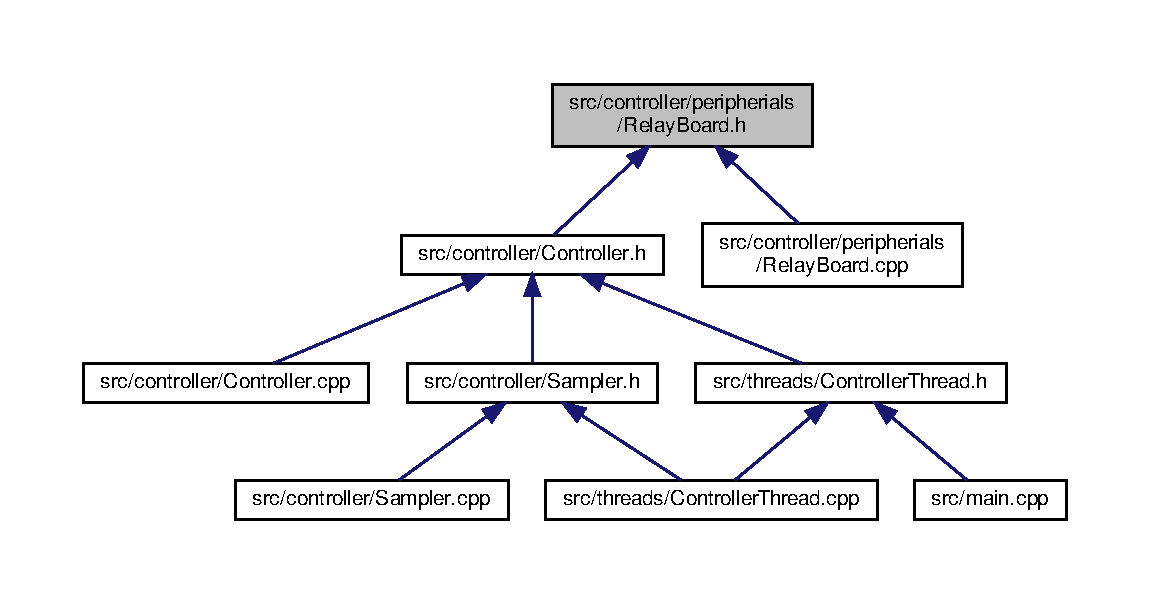
\includegraphics[width=350pt]{RelayBoard_8h__dep__incl}
\end{center}
\end{figure}
\subsection*{Classes}
\begin{DoxyCompactItemize}
\item 
class \hyperlink{classRelayBoard}{Relay\+Board}
\begin{DoxyCompactList}\small\item\em Relay Board class. \end{DoxyCompactList}\end{DoxyCompactItemize}


\subsection{Detailed Description}
\begin{DoxyAuthor}{Author}
Kamil Rog 
\end{DoxyAuthor}
\begin{DoxyVersion}{Version}
0.\+1
\end{DoxyVersion}
This header file contains the Elego relay board class. 
\hypertarget{SGP30_8cpp}{}\section{src/controller/peripherials/\+S\+G\+P30.cpp File Reference}
\label{SGP30_8cpp}\index{src/controller/peripherials/\+S\+G\+P30.\+cpp@{src/controller/peripherials/\+S\+G\+P30.\+cpp}}
{\ttfamily \#include $<$stdio.\+h$>$}\newline
{\ttfamily \#include \char`\"{}I2\+C\+Driver.\+h\char`\"{}}\newline
{\ttfamily \#include \char`\"{}S\+G\+P30.\+h\char`\"{}}\newline
Include dependency graph for S\+G\+P30.\+cpp\+:\nopagebreak
\begin{figure}[H]
\begin{center}
\leavevmode
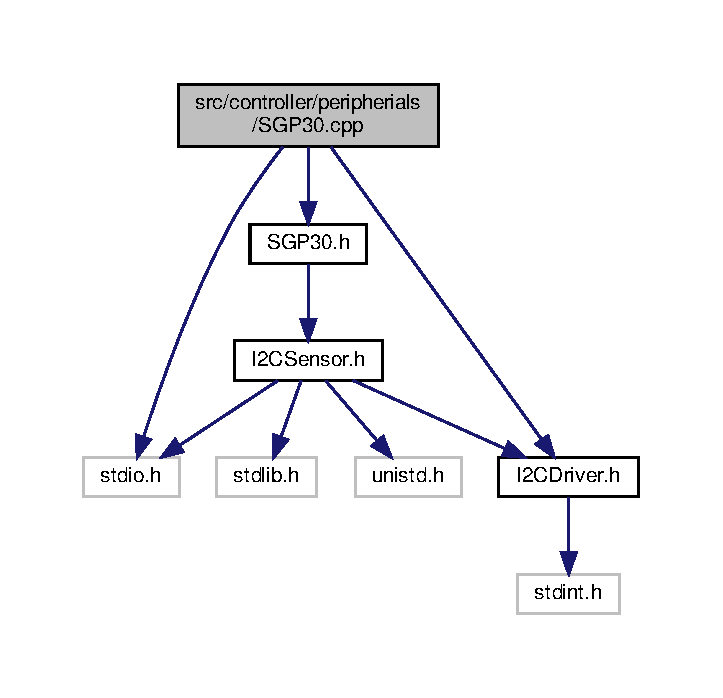
\includegraphics[width=347pt]{SGP30_8cpp__incl}
\end{center}
\end{figure}


\subsection{Detailed Description}
\begin{DoxyAuthor}{Author}
Kamil Rog 
\end{DoxyAuthor}
\begin{DoxyVersion}{Version}
0.\+1
\end{DoxyVersion}
This file contains the functions for \hyperlink{classSGP30}{S\+G\+P30} class. 
\hypertarget{SGP30_8h}{}\section{src/controller/peripherials/\+S\+G\+P30.h File Reference}
\label{SGP30_8h}\index{src/controller/peripherials/\+S\+G\+P30.\+h@{src/controller/peripherials/\+S\+G\+P30.\+h}}
{\ttfamily \#include \char`\"{}I2\+C\+Sensor.\+h\char`\"{}}\newline
Include dependency graph for S\+G\+P30.\+h\+:\nopagebreak
\begin{figure}[H]
\begin{center}
\leavevmode
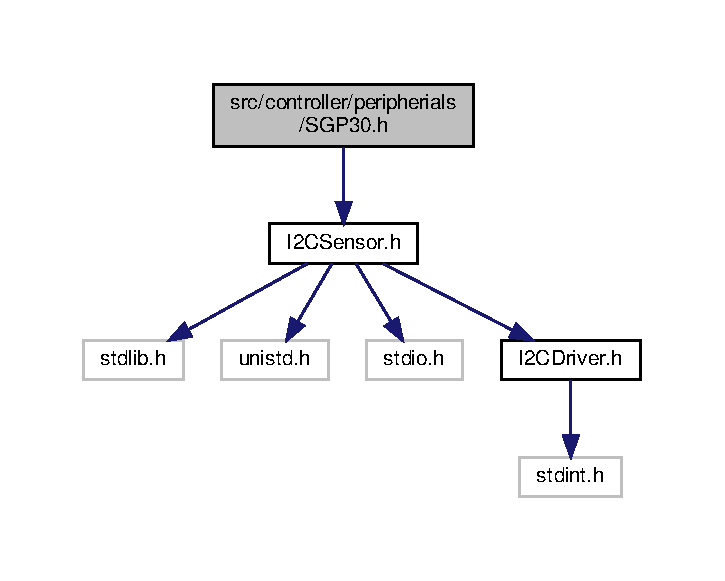
\includegraphics[width=348pt]{SGP30_8h__incl}
\end{center}
\end{figure}
This graph shows which files directly or indirectly include this file\+:\nopagebreak
\begin{figure}[H]
\begin{center}
\leavevmode
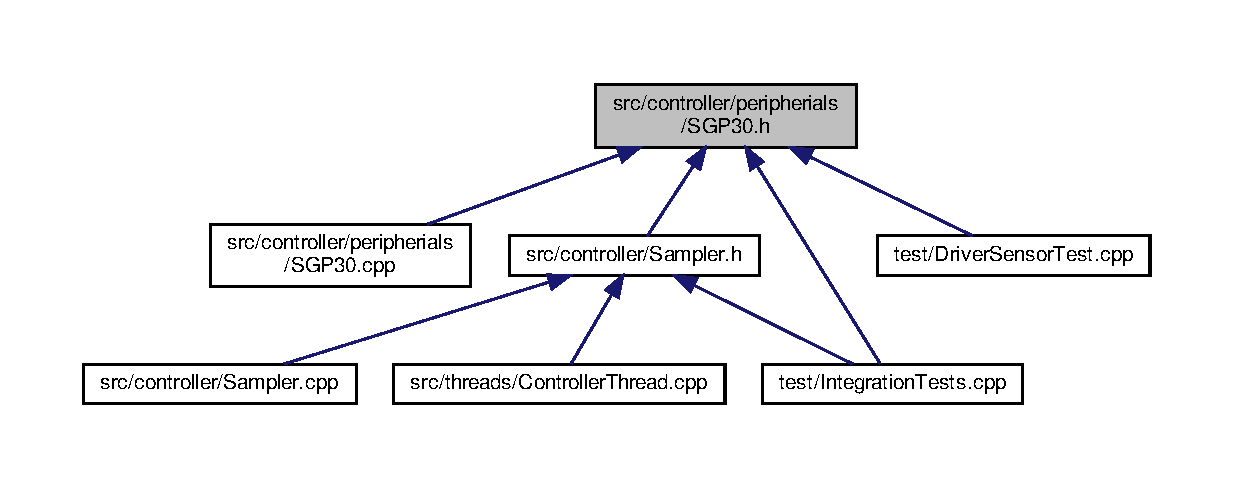
\includegraphics[width=350pt]{SGP30_8h__dep__incl}
\end{center}
\end{figure}
\subsection*{Classes}
\begin{DoxyCompactItemize}
\item 
class \hyperlink{classSGP30}{S\+G\+P30}
\begin{DoxyCompactList}\small\item\em \hyperlink{classSGP30}{S\+G\+P30} class. \end{DoxyCompactList}\end{DoxyCompactItemize}


\subsection{Detailed Description}
\begin{DoxyAuthor}{Author}
Kamil Rog 
\end{DoxyAuthor}
\begin{DoxyVersion}{Version}
0.\+1
\end{DoxyVersion}
This header file contains the class for \hyperlink{classSGP30}{S\+G\+P30} gas sensor. 
\hypertarget{SHT31D_8cpp}{}\section{src/controller/peripherials/\+S\+H\+T31D.cpp File Reference}
\label{SHT31D_8cpp}\index{src/controller/peripherials/\+S\+H\+T31\+D.\+cpp@{src/controller/peripherials/\+S\+H\+T31\+D.\+cpp}}
{\ttfamily \#include $<$stdio.\+h$>$}\newline
{\ttfamily \#include \char`\"{}S\+H\+T31\+D.\+h\char`\"{}}\newline
{\ttfamily \#include \char`\"{}I2\+C\+Driver.\+h\char`\"{}}\newline
Include dependency graph for S\+H\+T31\+D.\+cpp\+:\nopagebreak
\begin{figure}[H]
\begin{center}
\leavevmode
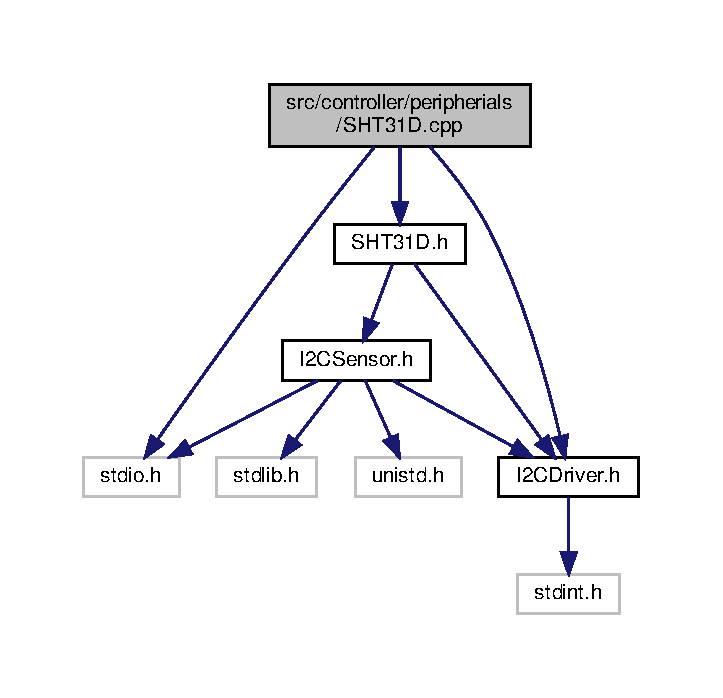
\includegraphics[width=347pt]{SHT31D_8cpp__incl}
\end{center}
\end{figure}


\subsection{Detailed Description}
\begin{DoxyAuthor}{Author}
Kamil Rog 
\end{DoxyAuthor}
\begin{DoxyVersion}{Version}
0.\+1
\end{DoxyVersion}
This file contains the functions for \hyperlink{classSHT31D}{S\+H\+T31D} class. 
\hypertarget{SHT31D_8h}{}\section{src/controller/peripherials/\+S\+H\+T31D.h File Reference}
\label{SHT31D_8h}\index{src/controller/peripherials/\+S\+H\+T31\+D.\+h@{src/controller/peripherials/\+S\+H\+T31\+D.\+h}}
{\ttfamily \#include \char`\"{}I2\+C\+Driver.\+h\char`\"{}}\newline
{\ttfamily \#include \char`\"{}I2\+C\+Sensor.\+h\char`\"{}}\newline
Include dependency graph for S\+H\+T31\+D.\+h\+:\nopagebreak
\begin{figure}[H]
\begin{center}
\leavevmode
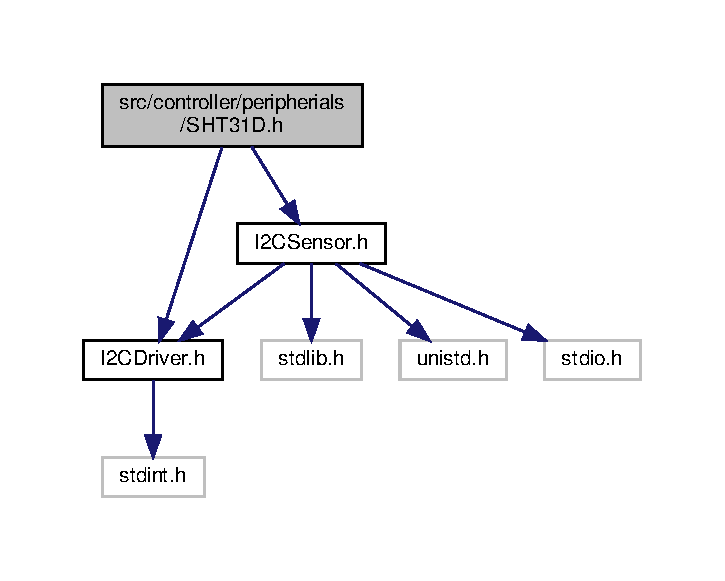
\includegraphics[width=348pt]{SHT31D_8h__incl}
\end{center}
\end{figure}
This graph shows which files directly or indirectly include this file\+:\nopagebreak
\begin{figure}[H]
\begin{center}
\leavevmode
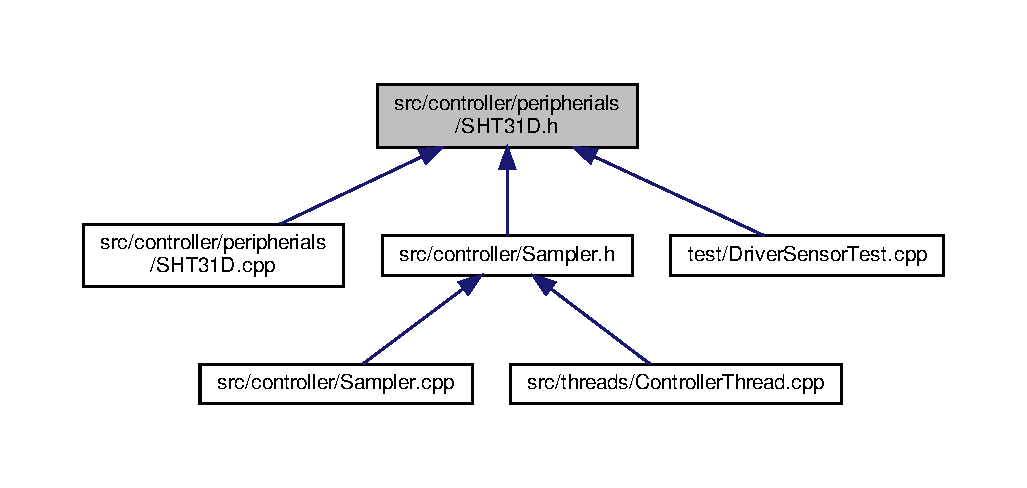
\includegraphics[width=350pt]{SHT31D_8h__dep__incl}
\end{center}
\end{figure}
\subsection*{Classes}
\begin{DoxyCompactItemize}
\item 
class \hyperlink{classSHT31D}{S\+H\+T31D}
\begin{DoxyCompactList}\small\item\em \hyperlink{classSHT31D}{S\+H\+T31D} class. \end{DoxyCompactList}\end{DoxyCompactItemize}
\subsection*{Macros}
\begin{DoxyCompactItemize}
\item 
\#define \hyperlink{SHT31D_8h_a5ed2621e822cb811383321e319ce3ee4}{S\+H\+T31\+D\+\_\+\+H\+A\+CK}~1
\end{DoxyCompactItemize}


\subsection{Detailed Description}
\begin{DoxyAuthor}{Author}
Kamil Rog 
\end{DoxyAuthor}
\begin{DoxyVersion}{Version}
0.\+1
\end{DoxyVersion}
This header file contains the class for the S\+H31D Sensor

This is a Temperature and Humidity sensor Currently The sensors must be written to in order to respond. A Hack has been implemented to write dummy data during initalization to overcome this issue 

\subsection{Macro Definition Documentation}
\mbox{\Hypertarget{SHT31D_8h_a5ed2621e822cb811383321e319ce3ee4}\label{SHT31D_8h_a5ed2621e822cb811383321e319ce3ee4}} 
\index{S\+H\+T31\+D.\+h@{S\+H\+T31\+D.\+h}!S\+H\+T31\+D\+\_\+\+H\+A\+CK@{S\+H\+T31\+D\+\_\+\+H\+A\+CK}}
\index{S\+H\+T31\+D\+\_\+\+H\+A\+CK@{S\+H\+T31\+D\+\_\+\+H\+A\+CK}!S\+H\+T31\+D.\+h@{S\+H\+T31\+D.\+h}}
\subsubsection{\texorpdfstring{S\+H\+T31\+D\+\_\+\+H\+A\+CK}{SHT31D\_HACK}}
{\footnotesize\ttfamily \#define S\+H\+T31\+D\+\_\+\+H\+A\+CK~1}


\hypertarget{VEML7700_8cpp}{}\section{src/controller/peripherials/\+V\+E\+M\+L7700.cpp File Reference}
\label{VEML7700_8cpp}\index{src/controller/peripherials/\+V\+E\+M\+L7700.\+cpp@{src/controller/peripherials/\+V\+E\+M\+L7700.\+cpp}}
{\ttfamily \#include \char`\"{}V\+E\+M\+L7700.\+h\char`\"{}}\newline
{\ttfamily \#include $<$cmath$>$}\newline
Include dependency graph for V\+E\+M\+L7700.\+cpp\+:\nopagebreak
\begin{figure}[H]
\begin{center}
\leavevmode
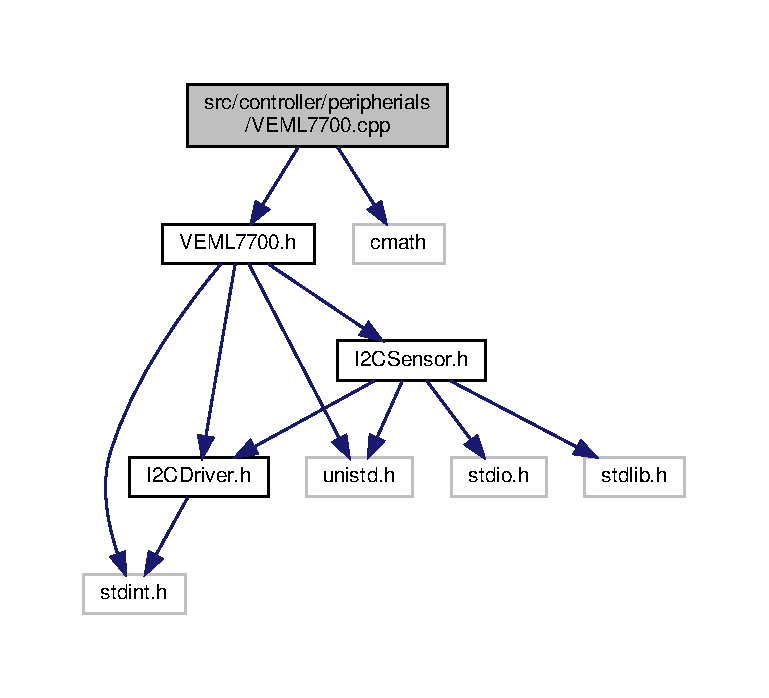
\includegraphics[width=350pt]{VEML7700_8cpp__incl}
\end{center}
\end{figure}


\subsection{Detailed Description}
\begin{DoxyAuthor}{Author}
Kamil Rog 
\end{DoxyAuthor}
\begin{DoxyVersion}{Version}
0.\+1
\end{DoxyVersion}
This file contains the functions for \hyperlink{classVEML7700}{V\+E\+M\+L7700} class. 
\hypertarget{VEML7700_8h}{}\section{src/controller/peripherials/\+V\+E\+M\+L7700.h File Reference}
\label{VEML7700_8h}\index{src/controller/peripherials/\+V\+E\+M\+L7700.\+h@{src/controller/peripherials/\+V\+E\+M\+L7700.\+h}}
{\ttfamily \#include $<$stdint.\+h$>$}\newline
{\ttfamily \#include $<$unistd.\+h$>$}\newline
{\ttfamily \#include \char`\"{}I2\+C\+Driver.\+h\char`\"{}}\newline
{\ttfamily \#include \char`\"{}I2\+C\+Sensor.\+h\char`\"{}}\newline
Include dependency graph for V\+E\+M\+L7700.\+h\+:\nopagebreak
\begin{figure}[H]
\begin{center}
\leavevmode
\includegraphics[width=350pt]{VEML7700_8h__incl}
\end{center}
\end{figure}
This graph shows which files directly or indirectly include this file\+:\nopagebreak
\begin{figure}[H]
\begin{center}
\leavevmode
\includegraphics[width=350pt]{VEML7700_8h__dep__incl}
\end{center}
\end{figure}
\subsection*{Classes}
\begin{DoxyCompactItemize}
\item 
class \hyperlink{classVEML7700}{V\+E\+M\+L7700}
\begin{DoxyCompactList}\small\item\em \hyperlink{classVEML7700}{V\+E\+M\+L7700} class. \end{DoxyCompactList}\end{DoxyCompactItemize}
\subsection*{Enumerations}
\begin{DoxyCompactItemize}
\item 
enum \{ \hyperlink{VEML7700_8h_aae05225933a42f81e7c4a9fb286596f9a7e4a42e3b6dd63708c64cf3db6f69566}{S\+T\+A\+T\+U\+S\+\_\+\+OK} = 0, 
\hyperlink{VEML7700_8h_aae05225933a42f81e7c4a9fb286596f9a5bde228d9506a863d51ffbc868ff67f7}{S\+T\+A\+T\+U\+S\+\_\+\+E\+R\+R\+OR} = -\/1
 \}
\end{DoxyCompactItemize}


\subsection{Detailed Description}
\begin{DoxyAuthor}{Author}
Kamil Rog 
\end{DoxyAuthor}
\begin{DoxyVersion}{Version}
0.\+1
\end{DoxyVersion}
This file contains the class for the \hyperlink{classVEML7700}{V\+E\+M\+L7700} A light sensor 

\subsection{Enumeration Type Documentation}
\mbox{\Hypertarget{VEML7700_8h_aae05225933a42f81e7c4a9fb286596f9}\label{VEML7700_8h_aae05225933a42f81e7c4a9fb286596f9}} 
\subsubsection{\texorpdfstring{anonymous enum}{anonymous enum}}
{\footnotesize\ttfamily anonymous enum}

Status Enumeration \begin{DoxyEnumFields}{Enumerator}
\raisebox{\heightof{T}}[0pt][0pt]{\index{S\+T\+A\+T\+U\+S\+\_\+\+OK@{S\+T\+A\+T\+U\+S\+\_\+\+OK}!V\+E\+M\+L7700.\+h@{V\+E\+M\+L7700.\+h}}\index{V\+E\+M\+L7700.\+h@{V\+E\+M\+L7700.\+h}!S\+T\+A\+T\+U\+S\+\_\+\+OK@{S\+T\+A\+T\+U\+S\+\_\+\+OK}}}\mbox{\Hypertarget{VEML7700_8h_aae05225933a42f81e7c4a9fb286596f9a7e4a42e3b6dd63708c64cf3db6f69566}\label{VEML7700_8h_aae05225933a42f81e7c4a9fb286596f9a7e4a42e3b6dd63708c64cf3db6f69566}} 
S\+T\+A\+T\+U\+S\+\_\+\+OK&\\
\hline

\raisebox{\heightof{T}}[0pt][0pt]{\index{S\+T\+A\+T\+U\+S\+\_\+\+E\+R\+R\+OR@{S\+T\+A\+T\+U\+S\+\_\+\+E\+R\+R\+OR}!V\+E\+M\+L7700.\+h@{V\+E\+M\+L7700.\+h}}\index{V\+E\+M\+L7700.\+h@{V\+E\+M\+L7700.\+h}!S\+T\+A\+T\+U\+S\+\_\+\+E\+R\+R\+OR@{S\+T\+A\+T\+U\+S\+\_\+\+E\+R\+R\+OR}}}\mbox{\Hypertarget{VEML7700_8h_aae05225933a42f81e7c4a9fb286596f9a5bde228d9506a863d51ffbc868ff67f7}\label{VEML7700_8h_aae05225933a42f81e7c4a9fb286596f9a5bde228d9506a863d51ffbc868ff67f7}} 
S\+T\+A\+T\+U\+S\+\_\+\+E\+R\+R\+OR&\\
\hline

\end{DoxyEnumFields}

\hypertarget{Sampler_8cpp}{}\section{src/controller/\+Sampler.cpp File Reference}
\label{Sampler_8cpp}\index{src/controller/\+Sampler.\+cpp@{src/controller/\+Sampler.\+cpp}}
{\ttfamily \#include \char`\"{}Sampler.\+h\char`\"{}}\newline
{\ttfamily \#include $<$stdio.\+h$>$}\newline
{\ttfamily \#include $<$unistd.\+h$>$}\newline
Include dependency graph for Sampler.\+cpp\+:
\nopagebreak
\begin{figure}[H]
\begin{center}
\leavevmode
\includegraphics[width=350pt]{Sampler_8cpp__incl}
\end{center}
\end{figure}


\subsection{Detailed Description}
\begin{DoxyAuthor}{Author}
Kamil Rog 
\end{DoxyAuthor}
\begin{DoxyVersion}{Version}
0.\+1
\end{DoxyVersion}
This file contains the function for controller class. 
\hypertarget{Sampler_8h}{}\section{src/controller/\+Sampler.h File Reference}
\label{Sampler_8h}\index{src/controller/\+Sampler.\+h@{src/controller/\+Sampler.\+h}}
{\ttfamily \#include \char`\"{}Controller.\+h\char`\"{}}\newline
{\ttfamily \#include $<$stdio.\+h$>$}\newline
{\ttfamily \#include \char`\"{}Cpp\+Timer.\+h\char`\"{}}\newline
{\ttfamily \#include \char`\"{}I2\+C\+Driver.\+h\char`\"{}}\newline
{\ttfamily \#include \char`\"{}I2\+C\+Sensor.\+h\char`\"{}}\newline
{\ttfamily \#include \char`\"{}V\+E\+M\+L7700.\+h\char`\"{}}\newline
{\ttfamily \#include \char`\"{}S\+H\+T31\+D.\+h\char`\"{}}\newline
{\ttfamily \#include \char`\"{}S\+G\+P30.\+h\char`\"{}}\newline
Include dependency graph for Sampler.\+h\+:
\nopagebreak
\begin{figure}[H]
\begin{center}
\leavevmode
\includegraphics[width=350pt]{Sampler_8h__incl}
\end{center}
\end{figure}
This graph shows which files directly or indirectly include this file\+:
\nopagebreak
\begin{figure}[H]
\begin{center}
\leavevmode
\includegraphics[width=350pt]{Sampler_8h__dep__incl}
\end{center}
\end{figure}
\subsection*{Classes}
\begin{DoxyCompactItemize}
\item 
class \hyperlink{classSampler}{Sampler}
\begin{DoxyCompactList}\small\item\em \hyperlink{classSampler}{Sampler} Class. \end{DoxyCompactList}\end{DoxyCompactItemize}


\subsection{Detailed Description}
\begin{DoxyAuthor}{Author}
Kamil Rog 
\end{DoxyAuthor}
\begin{DoxyVersion}{Version}
0.\+1
\end{DoxyVersion}
This header file contains the thread for \hyperlink{classController}{Controller} of the Agro\+Pi sensors and actuators 
\hypertarget{ControllerThread_8cpp}{}\section{src/threads/\+Controller\+Thread.cpp File Reference}
\label{ControllerThread_8cpp}\index{src/threads/\+Controller\+Thread.\+cpp@{src/threads/\+Controller\+Thread.\+cpp}}
{\ttfamily \#include \char`\"{}json\+\_\+fastcgi\+\_\+web\+\_\+api.\+h\char`\"{}}\newline
{\ttfamily \#include \char`\"{}Controller\+Thread.\+h\char`\"{}}\newline
{\ttfamily \#include \char`\"{}Sampler.\+h\char`\"{}}\newline
{\ttfamily \#include \char`\"{}Camera.\+h\char`\"{}}\newline
{\ttfamily \#include $<$stdio.\+h$>$}\newline
{\ttfamily \#include $<$chrono$>$}\newline
{\ttfamily \#include $<$mutex$>$}\newline
{\ttfamily \#include $<$sstream$>$}\newline
{\ttfamily \#include $<$thread$>$}\newline
Include dependency graph for Controller\+Thread.\+cpp\+:
\nopagebreak
\begin{figure}[H]
\begin{center}
\leavevmode
\includegraphics[width=350pt]{ControllerThread_8cpp__incl}
\end{center}
\end{figure}
\subsection*{Classes}
\begin{DoxyCompactItemize}
\item 
class \hyperlink{classJSONCGIDataCallback}{J\+S\+O\+N\+C\+G\+I\+Data\+Callback}
\item 
class \hyperlink{classControllerCallback}{Controller\+Callback}
\end{DoxyCompactItemize}
\subsection*{Enumerations}
\begin{DoxyCompactItemize}
\item 
enum \hyperlink{ControllerThread_8cpp_a60176172068ee7057c3fd49521dd0115}{E\+V\+E\+N\+T\+\_\+\+O\+P\+\_\+\+C\+O\+D\+ES} \{ \hyperlink{ControllerThread_8cpp_a60176172068ee7057c3fd49521dd0115ae5c39d7ebc2e5d0ea28b531d983d9731}{S\+A\+M\+P\+L\+E\+\_\+\+R\+A\+T\+E\+\_\+\+C\+H\+A\+N\+GE} = 253, 
\hyperlink{ControllerThread_8cpp_a60176172068ee7057c3fd49521dd0115a97bb101d1d6c18d26fe95f18cef3792d}{E\+N\+A\+B\+L\+E\+\_\+\+S\+A\+M\+P\+L\+I\+NG} = 254, 
\hyperlink{ControllerThread_8cpp_a60176172068ee7057c3fd49521dd0115a945280aa3e9db0f24215a8d9b6ddbd8e}{E\+X\+I\+T\+\_\+\+A\+P\+P\+L\+I\+C\+A\+T\+I\+ON} = 255
 \}
\end{DoxyCompactItemize}
\subsection*{Functions}
\begin{DoxyCompactItemize}
\item 
void \hyperlink{ControllerThread_8cpp_a844160e16f1a3e514df9ce65683e17bd}{sig\+Handler} (int sig)
\item 
void \hyperlink{ControllerThread_8cpp_a20a45737018ec41ab19cb4f5164b26ac}{set\+H\+U\+P\+Handler} ()
\end{DoxyCompactItemize}
\subsection*{Variables}
\begin{DoxyCompactItemize}
\item 
int \hyperlink{ControllerThread_8cpp_a94a2e79f236e50a73fb8c842bcff7738}{main\+Running} = 1
\end{DoxyCompactItemize}


\subsection{Detailed Description}
\begin{DoxyAuthor}{Author}
Kamil Rog 
\end{DoxyAuthor}
\begin{DoxyVersion}{Version}
0.\+1
\end{DoxyVersion}
This file contains the functions for Server Thread class. 

\subsection{Enumeration Type Documentation}
\mbox{\Hypertarget{ControllerThread_8cpp_a60176172068ee7057c3fd49521dd0115}\label{ControllerThread_8cpp_a60176172068ee7057c3fd49521dd0115}} 
\index{Controller\+Thread.\+cpp@{Controller\+Thread.\+cpp}!E\+V\+E\+N\+T\+\_\+\+O\+P\+\_\+\+C\+O\+D\+ES@{E\+V\+E\+N\+T\+\_\+\+O\+P\+\_\+\+C\+O\+D\+ES}}
\index{E\+V\+E\+N\+T\+\_\+\+O\+P\+\_\+\+C\+O\+D\+ES@{E\+V\+E\+N\+T\+\_\+\+O\+P\+\_\+\+C\+O\+D\+ES}!Controller\+Thread.\+cpp@{Controller\+Thread.\+cpp}}
\subsubsection{\texorpdfstring{E\+V\+E\+N\+T\+\_\+\+O\+P\+\_\+\+C\+O\+D\+ES}{EVENT\_OP\_CODES}}
{\footnotesize\ttfamily enum \hyperlink{ControllerThread_8cpp_a60176172068ee7057c3fd49521dd0115}{E\+V\+E\+N\+T\+\_\+\+O\+P\+\_\+\+C\+O\+D\+ES}}

\begin{DoxyEnumFields}{Enumerator}
\raisebox{\heightof{T}}[0pt][0pt]{\index{S\+A\+M\+P\+L\+E\+\_\+\+R\+A\+T\+E\+\_\+\+C\+H\+A\+N\+GE@{S\+A\+M\+P\+L\+E\+\_\+\+R\+A\+T\+E\+\_\+\+C\+H\+A\+N\+GE}!Controller\+Thread.\+cpp@{Controller\+Thread.\+cpp}}\index{Controller\+Thread.\+cpp@{Controller\+Thread.\+cpp}!S\+A\+M\+P\+L\+E\+\_\+\+R\+A\+T\+E\+\_\+\+C\+H\+A\+N\+GE@{S\+A\+M\+P\+L\+E\+\_\+\+R\+A\+T\+E\+\_\+\+C\+H\+A\+N\+GE}}}\mbox{\Hypertarget{ControllerThread_8cpp_a60176172068ee7057c3fd49521dd0115ae5c39d7ebc2e5d0ea28b531d983d9731}\label{ControllerThread_8cpp_a60176172068ee7057c3fd49521dd0115ae5c39d7ebc2e5d0ea28b531d983d9731}} 
S\+A\+M\+P\+L\+E\+\_\+\+R\+A\+T\+E\+\_\+\+C\+H\+A\+N\+GE&\\
\hline

\raisebox{\heightof{T}}[0pt][0pt]{\index{E\+N\+A\+B\+L\+E\+\_\+\+S\+A\+M\+P\+L\+I\+NG@{E\+N\+A\+B\+L\+E\+\_\+\+S\+A\+M\+P\+L\+I\+NG}!Controller\+Thread.\+cpp@{Controller\+Thread.\+cpp}}\index{Controller\+Thread.\+cpp@{Controller\+Thread.\+cpp}!E\+N\+A\+B\+L\+E\+\_\+\+S\+A\+M\+P\+L\+I\+NG@{E\+N\+A\+B\+L\+E\+\_\+\+S\+A\+M\+P\+L\+I\+NG}}}\mbox{\Hypertarget{ControllerThread_8cpp_a60176172068ee7057c3fd49521dd0115a97bb101d1d6c18d26fe95f18cef3792d}\label{ControllerThread_8cpp_a60176172068ee7057c3fd49521dd0115a97bb101d1d6c18d26fe95f18cef3792d}} 
E\+N\+A\+B\+L\+E\+\_\+\+S\+A\+M\+P\+L\+I\+NG&\\
\hline

\raisebox{\heightof{T}}[0pt][0pt]{\index{E\+X\+I\+T\+\_\+\+A\+P\+P\+L\+I\+C\+A\+T\+I\+ON@{E\+X\+I\+T\+\_\+\+A\+P\+P\+L\+I\+C\+A\+T\+I\+ON}!Controller\+Thread.\+cpp@{Controller\+Thread.\+cpp}}\index{Controller\+Thread.\+cpp@{Controller\+Thread.\+cpp}!E\+X\+I\+T\+\_\+\+A\+P\+P\+L\+I\+C\+A\+T\+I\+ON@{E\+X\+I\+T\+\_\+\+A\+P\+P\+L\+I\+C\+A\+T\+I\+ON}}}\mbox{\Hypertarget{ControllerThread_8cpp_a60176172068ee7057c3fd49521dd0115a945280aa3e9db0f24215a8d9b6ddbd8e}\label{ControllerThread_8cpp_a60176172068ee7057c3fd49521dd0115a945280aa3e9db0f24215a8d9b6ddbd8e}} 
E\+X\+I\+T\+\_\+\+A\+P\+P\+L\+I\+C\+A\+T\+I\+ON&\\
\hline

\end{DoxyEnumFields}


\subsection{Function Documentation}
\mbox{\Hypertarget{ControllerThread_8cpp_a20a45737018ec41ab19cb4f5164b26ac}\label{ControllerThread_8cpp_a20a45737018ec41ab19cb4f5164b26ac}} 
\index{Controller\+Thread.\+cpp@{Controller\+Thread.\+cpp}!set\+H\+U\+P\+Handler@{set\+H\+U\+P\+Handler}}
\index{set\+H\+U\+P\+Handler@{set\+H\+U\+P\+Handler}!Controller\+Thread.\+cpp@{Controller\+Thread.\+cpp}}
\subsubsection{\texorpdfstring{set\+H\+U\+P\+Handler()}{setHUPHandler()}}
{\footnotesize\ttfamily void set\+H\+U\+P\+Handler (\begin{DoxyParamCaption}{ }\end{DoxyParamCaption})}

Sets a signal handler so that you can kill the background process gracefully with\+: kill -\/\+H\+UP $<$\+P\+I\+D$>$ \mbox{\Hypertarget{ControllerThread_8cpp_a844160e16f1a3e514df9ce65683e17bd}\label{ControllerThread_8cpp_a844160e16f1a3e514df9ce65683e17bd}} 
\index{Controller\+Thread.\+cpp@{Controller\+Thread.\+cpp}!sig\+Handler@{sig\+Handler}}
\index{sig\+Handler@{sig\+Handler}!Controller\+Thread.\+cpp@{Controller\+Thread.\+cpp}}
\subsubsection{\texorpdfstring{sig\+Handler()}{sigHandler()}}
{\footnotesize\ttfamily void sig\+Handler (\begin{DoxyParamCaption}\item[{int}]{sig }\end{DoxyParamCaption})}

Handler when the user has pressed ctrl-\/C send H\+UP via the kill command. 

\subsection{Variable Documentation}
\mbox{\Hypertarget{ControllerThread_8cpp_a94a2e79f236e50a73fb8c842bcff7738}\label{ControllerThread_8cpp_a94a2e79f236e50a73fb8c842bcff7738}} 
\index{Controller\+Thread.\+cpp@{Controller\+Thread.\+cpp}!main\+Running@{main\+Running}}
\index{main\+Running@{main\+Running}!Controller\+Thread.\+cpp@{Controller\+Thread.\+cpp}}
\subsubsection{\texorpdfstring{main\+Running}{mainRunning}}
{\footnotesize\ttfamily int main\+Running = 1}

Flag to indicate program is running. Needed later to quit the idle loop. 
\hypertarget{ControllerThread_8h}{}\section{src/threads/\+Controller\+Thread.h File Reference}
\label{ControllerThread_8h}\index{src/threads/\+Controller\+Thread.\+h@{src/threads/\+Controller\+Thread.\+h}}
{\ttfamily \#include \char`\"{}Cpp\+Thread.\+h\char`\"{}}\newline
{\ttfamily \#include \char`\"{}Controller.\+h\char`\"{}}\newline
Include dependency graph for Controller\+Thread.\+h\+:\nopagebreak
\begin{figure}[H]
\begin{center}
\leavevmode
\includegraphics[width=350pt]{ControllerThread_8h__incl}
\end{center}
\end{figure}
This graph shows which files directly or indirectly include this file\+:\nopagebreak
\begin{figure}[H]
\begin{center}
\leavevmode
\includegraphics[width=330pt]{ControllerThread_8h__dep__incl}
\end{center}
\end{figure}
\subsection*{Classes}
\begin{DoxyCompactItemize}
\item 
class \hyperlink{classControllerThread}{Controller\+Thread}
\begin{DoxyCompactList}\small\item\em Server Thread class. \end{DoxyCompactList}\end{DoxyCompactItemize}


\subsection{Detailed Description}
\begin{DoxyAuthor}{Author}
Kamil Rog 
\end{DoxyAuthor}
\begin{DoxyVersion}{Version}
0.\+1
\end{DoxyVersion}
This header file contains the definition for server thread for 
\hypertarget{CppThread_8h}{}\section{src/threads/\+Cpp\+Thread.h File Reference}
\label{CppThread_8h}\index{src/threads/\+Cpp\+Thread.\+h@{src/threads/\+Cpp\+Thread.\+h}}
{\ttfamily \#include $<$thread$>$}\newline
Include dependency graph for Cpp\+Thread.\+h\+:\nopagebreak
\begin{figure}[H]
\begin{center}
\leavevmode
\includegraphics[width=205pt]{CppThread_8h__incl}
\end{center}
\end{figure}
This graph shows which files directly or indirectly include this file\+:\nopagebreak
\begin{figure}[H]
\begin{center}
\leavevmode
\includegraphics[width=330pt]{CppThread_8h__dep__incl}
\end{center}
\end{figure}
\subsection*{Classes}
\begin{DoxyCompactItemize}
\item 
class \hyperlink{classCppThread}{Cpp\+Thread}
\end{DoxyCompactItemize}

\hypertarget{CppTimer_8cpp}{}\section{src/utils/\+Cpp\+Timer.cpp File Reference}
\label{CppTimer_8cpp}\index{src/utils/\+Cpp\+Timer.\+cpp@{src/utils/\+Cpp\+Timer.\+cpp}}
{\ttfamily \#include \char`\"{}Cpp\+Timer.\+h\char`\"{}}\newline
Include dependency graph for Cpp\+Timer.\+cpp\+:\nopagebreak
\begin{figure}[H]
\begin{center}
\leavevmode
\includegraphics[width=350pt]{CppTimer_8cpp__incl}
\end{center}
\end{figure}

\hypertarget{CppTimer_8h}{}\section{src/utils/\+Cpp\+Timer.h File Reference}
\label{CppTimer_8h}\index{src/utils/\+Cpp\+Timer.\+h@{src/utils/\+Cpp\+Timer.\+h}}
{\ttfamily \#include $<$stdlib.\+h$>$}\newline
{\ttfamily \#include $<$unistd.\+h$>$}\newline
{\ttfamily \#include $<$stdio.\+h$>$}\newline
{\ttfamily \#include $<$signal.\+h$>$}\newline
{\ttfamily \#include $<$time.\+h$>$}\newline
Include dependency graph for Cpp\+Timer.\+h\+:\nopagebreak
\begin{figure}[H]
\begin{center}
\leavevmode
\includegraphics[width=350pt]{CppTimer_8h__incl}
\end{center}
\end{figure}
This graph shows which files directly or indirectly include this file\+:\nopagebreak
\begin{figure}[H]
\begin{center}
\leavevmode
\includegraphics[width=350pt]{CppTimer_8h__dep__incl}
\end{center}
\end{figure}
\subsection*{Classes}
\begin{DoxyCompactItemize}
\item 
class \hyperlink{classCppTimer}{Cpp\+Timer}
\end{DoxyCompactItemize}
\subsection*{Macros}
\begin{DoxyCompactItemize}
\item 
\#define \hyperlink{CppTimer_8h_a2694a39dfd1fa087ca6f9f391c91dae7}{C\+L\+O\+C\+K\+ID}~C\+L\+O\+C\+K\+\_\+\+M\+O\+N\+O\+T\+O\+N\+IC
\item 
\#define \hyperlink{CppTimer_8h_ad6f1d374549d22100d676d5fcac0a7e5}{S\+IG}~S\+I\+G\+R\+T\+M\+IN
\end{DoxyCompactItemize}
\subsection*{Typedefs}
\begin{DoxyCompactItemize}
\item 
typedef enum \hyperlink{CppTimer_8h_a110d07ab6a96d7815149d3d95435790a}{cpp\+Timer\+Type\+\_\+t} \hyperlink{CppTimer_8h_a108f54b7f3f493de3e2e76a813447769}{cpp\+Timer\+Type\+\_\+t}
\end{DoxyCompactItemize}
\subsection*{Enumerations}
\begin{DoxyCompactItemize}
\item 
enum \hyperlink{CppTimer_8h_a110d07ab6a96d7815149d3d95435790a}{cpp\+Timer\+Type\+\_\+t} \{ \hyperlink{CppTimer_8h_a110d07ab6a96d7815149d3d95435790aae4379d044711537d9ce3b3b58c575c58}{P\+E\+R\+I\+O\+D\+IC}, 
\hyperlink{CppTimer_8h_a110d07ab6a96d7815149d3d95435790aa2724fa87f252403cd2c93f7437f34fd5}{O\+N\+E\+S\+H\+OT}
 \}
\end{DoxyCompactItemize}


\subsection{Macro Definition Documentation}
\mbox{\Hypertarget{CppTimer_8h_a2694a39dfd1fa087ca6f9f391c91dae7}\label{CppTimer_8h_a2694a39dfd1fa087ca6f9f391c91dae7}} 
\index{Cpp\+Timer.\+h@{Cpp\+Timer.\+h}!C\+L\+O\+C\+K\+ID@{C\+L\+O\+C\+K\+ID}}
\index{C\+L\+O\+C\+K\+ID@{C\+L\+O\+C\+K\+ID}!Cpp\+Timer.\+h@{Cpp\+Timer.\+h}}
\subsubsection{\texorpdfstring{C\+L\+O\+C\+K\+ID}{CLOCKID}}
{\footnotesize\ttfamily \#define C\+L\+O\+C\+K\+ID~C\+L\+O\+C\+K\+\_\+\+M\+O\+N\+O\+T\+O\+N\+IC}

G\+NU G\+E\+N\+E\+R\+AL P\+U\+B\+L\+IC L\+I\+C\+E\+N\+SE Version 3, 29 June 2007

(C) 2020, Bernd Porr \href{mailto:mail@bernporr.me.uk}{\tt mail@bernporr.\+me.\+uk}

This is inspired by the timer\+\_\+create man page. \mbox{\Hypertarget{CppTimer_8h_ad6f1d374549d22100d676d5fcac0a7e5}\label{CppTimer_8h_ad6f1d374549d22100d676d5fcac0a7e5}} 
\index{Cpp\+Timer.\+h@{Cpp\+Timer.\+h}!S\+IG@{S\+IG}}
\index{S\+IG@{S\+IG}!Cpp\+Timer.\+h@{Cpp\+Timer.\+h}}
\subsubsection{\texorpdfstring{S\+IG}{SIG}}
{\footnotesize\ttfamily \#define S\+IG~S\+I\+G\+R\+T\+M\+IN}



\subsection{Typedef Documentation}
\mbox{\Hypertarget{CppTimer_8h_a108f54b7f3f493de3e2e76a813447769}\label{CppTimer_8h_a108f54b7f3f493de3e2e76a813447769}} 
\index{Cpp\+Timer.\+h@{Cpp\+Timer.\+h}!cpp\+Timer\+Type\+\_\+t@{cpp\+Timer\+Type\+\_\+t}}
\index{cpp\+Timer\+Type\+\_\+t@{cpp\+Timer\+Type\+\_\+t}!Cpp\+Timer.\+h@{Cpp\+Timer.\+h}}
\subsubsection{\texorpdfstring{cpp\+Timer\+Type\+\_\+t}{cppTimerType\_t}}
{\footnotesize\ttfamily typedef enum \hyperlink{CppTimer_8h_a110d07ab6a96d7815149d3d95435790a}{cpp\+Timer\+Type\+\_\+t} \hyperlink{CppTimer_8h_a110d07ab6a96d7815149d3d95435790a}{cpp\+Timer\+Type\+\_\+t}}

Enumeration of \hyperlink{classCppTimer}{Cpp\+Timer} types 

\subsection{Enumeration Type Documentation}
\mbox{\Hypertarget{CppTimer_8h_a110d07ab6a96d7815149d3d95435790a}\label{CppTimer_8h_a110d07ab6a96d7815149d3d95435790a}} 
\index{Cpp\+Timer.\+h@{Cpp\+Timer.\+h}!cpp\+Timer\+Type\+\_\+t@{cpp\+Timer\+Type\+\_\+t}}
\index{cpp\+Timer\+Type\+\_\+t@{cpp\+Timer\+Type\+\_\+t}!Cpp\+Timer.\+h@{Cpp\+Timer.\+h}}
\subsubsection{\texorpdfstring{cpp\+Timer\+Type\+\_\+t}{cppTimerType\_t}}
{\footnotesize\ttfamily enum \hyperlink{CppTimer_8h_a110d07ab6a96d7815149d3d95435790a}{cpp\+Timer\+Type\+\_\+t}}

Enumeration of \hyperlink{classCppTimer}{Cpp\+Timer} types \begin{DoxyEnumFields}{Enumerator}
\raisebox{\heightof{T}}[0pt][0pt]{\index{P\+E\+R\+I\+O\+D\+IC@{P\+E\+R\+I\+O\+D\+IC}!Cpp\+Timer.\+h@{Cpp\+Timer.\+h}}\index{Cpp\+Timer.\+h@{Cpp\+Timer.\+h}!P\+E\+R\+I\+O\+D\+IC@{P\+E\+R\+I\+O\+D\+IC}}}\mbox{\Hypertarget{CppTimer_8h_a110d07ab6a96d7815149d3d95435790aae4379d044711537d9ce3b3b58c575c58}\label{CppTimer_8h_a110d07ab6a96d7815149d3d95435790aae4379d044711537d9ce3b3b58c575c58}} 
P\+E\+R\+I\+O\+D\+IC&\\
\hline

\raisebox{\heightof{T}}[0pt][0pt]{\index{O\+N\+E\+S\+H\+OT@{O\+N\+E\+S\+H\+OT}!Cpp\+Timer.\+h@{Cpp\+Timer.\+h}}\index{Cpp\+Timer.\+h@{Cpp\+Timer.\+h}!O\+N\+E\+S\+H\+OT@{O\+N\+E\+S\+H\+OT}}}\mbox{\Hypertarget{CppTimer_8h_a110d07ab6a96d7815149d3d95435790aa2724fa87f252403cd2c93f7437f34fd5}\label{CppTimer_8h_a110d07ab6a96d7815149d3d95435790aa2724fa87f252403cd2c93f7437f34fd5}} 
O\+N\+E\+S\+H\+OT&\\
\hline

\end{DoxyEnumFields}

\hypertarget{CppTimerCallback_8h}{}\section{src/utils/\+Cpp\+Timer\+Callback.h File Reference}
\label{CppTimerCallback_8h}\index{src/utils/\+Cpp\+Timer\+Callback.\+h@{src/utils/\+Cpp\+Timer\+Callback.\+h}}
{\ttfamily \#include $<$stdio.\+h$>$}\newline
{\ttfamily \#include \char`\"{}Cpp\+Timer.\+h\char`\"{}}\newline
{\ttfamily \#include $<$unistd.\+h$>$}\newline
Include dependency graph for Cpp\+Timer\+Callback.\+h\+:\nopagebreak
\begin{figure}[H]
\begin{center}
\leavevmode
\includegraphics[width=350pt]{CppTimerCallback_8h__incl}
\end{center}
\end{figure}
\subsection*{Classes}
\begin{DoxyCompactItemize}
\item 
class \hyperlink{classCppTimerCallback}{Cpp\+Timer\+Callback}
\item 
class \hyperlink{classCppTimerCallback_1_1Runnable}{Cpp\+Timer\+Callback\+::\+Runnable}
\end{DoxyCompactItemize}

\hypertarget{typeDefinitions_8h}{}\section{src/utils/type\+Definitions.h File Reference}
\label{typeDefinitions_8h}\index{src/utils/type\+Definitions.\+h@{src/utils/type\+Definitions.\+h}}
{\ttfamily \#include $<$unistd.\+h$>$}\newline
{\ttfamily \#include $<$stdint.\+h$>$}\newline
{\ttfamily \#include $<$stdio.\+h$>$}\newline
{\ttfamily \#include $<$stdlib.\+h$>$}\newline
Include dependency graph for type\+Definitions.\+h\+:\nopagebreak
\begin{figure}[H]
\begin{center}
\leavevmode
\includegraphics[width=329pt]{typeDefinitions_8h__incl}
\end{center}
\end{figure}
This graph shows which files directly or indirectly include this file\+:\nopagebreak
\begin{figure}[H]
\begin{center}
\leavevmode
\includegraphics[width=350pt]{typeDefinitions_8h__dep__incl}
\end{center}
\end{figure}
\subsection*{Classes}
\begin{DoxyCompactItemize}
\item 
struct \hyperlink{structEnvironmentData}{Environment\+Data}
\item 
struct \hyperlink{structTargetEnvironmentData}{Target\+Environment\+Data}
\item 
struct \hyperlink{structActuationForceFlags}{Actuation\+Force\+Flags}
\item 
struct \hyperlink{structActuationHeuristicsFlags}{Actuation\+Heuristics\+Flags}
\end{DoxyCompactItemize}

\hypertarget{utils_8cpp}{}\section{src/utils/utils.cpp File Reference}
\label{utils_8cpp}\index{src/utils/utils.\+cpp@{src/utils/utils.\+cpp}}
{\ttfamily \#include $<$unistd.\+h$>$}\newline
{\ttfamily \#include $<$stdint.\+h$>$}\newline
{\ttfamily \#include $<$stdio.\+h$>$}\newline
{\ttfamily \#include $<$stdlib.\+h$>$}\newline
Include dependency graph for utils.\+cpp\+:\nopagebreak
\begin{figure}[H]
\begin{center}
\leavevmode
\includegraphics[width=329pt]{utils_8cpp__incl}
\end{center}
\end{figure}
\subsection*{Functions}
\begin{DoxyCompactItemize}
\item 
uint8\+\_\+t \hyperlink{utils_8cpp_a382a50931a510e3f93461c289586dfd6}{C\+R\+C8} (uint8\+\_\+t $\ast$data, uint8\+\_\+t datalen)
\end{DoxyCompactItemize}


\subsection{Detailed Description}
\begin{DoxyAuthor}{Author}
Kamil Rog 
\end{DoxyAuthor}
\begin{DoxyVersion}{Version}
0.\+1
\end{DoxyVersion}
This file contains the utilities functions used in the project. 

\subsection{Function Documentation}
\mbox{\Hypertarget{utils_8cpp_a382a50931a510e3f93461c289586dfd6}\label{utils_8cpp_a382a50931a510e3f93461c289586dfd6}} 
\index{utils.\+cpp@{utils.\+cpp}!C\+R\+C8@{C\+R\+C8}}
\index{C\+R\+C8@{C\+R\+C8}!utils.\+cpp@{utils.\+cpp}}
\subsubsection{\texorpdfstring{C\+R\+C8()}{CRC8()}}
{\footnotesize\ttfamily uint8\+\_\+t C\+R\+C8 (\begin{DoxyParamCaption}\item[{uint8\+\_\+t $\ast$}]{data,  }\item[{uint8\+\_\+t}]{datalen }\end{DoxyParamCaption})}

Cyclic redundancy check, Calculates 8-\/\+Bit checksum with following parameters Specified on page 14 of \hyperlink{classSHT31D}{S\+H\+T31D} Application Note \& Also applies to \hyperlink{classSGP30}{S\+G\+P30} Initial value\+: 0x\+FF Polynomial\+: 0x31 (x$^\wedge$8 + x$^\wedge$5 + x$^\wedge$4 + 1) X\+OR Result by\+: 0x00


\begin{DoxyParams}{Parameters}
{\em data} & Data to perform C\+R\+C8 on \\
\hline
{\em datalen} & length of the data in bytes\\
\hline
\end{DoxyParams}
\begin{DoxyReturn}{Returns}
Byte C\+RC Checksum
\end{DoxyReturn}
\begin{DoxyRefDesc}{Todo}
\item[\hyperlink{todo__todo000003}{Todo}]\+: Modify to pass in polynomial, initial value and X\+OR factor \end{DoxyRefDesc}

\hypertarget{utils_8h}{}\section{src/utils/utils.h File Reference}
\label{utils_8h}\index{src/utils/utils.\+h@{src/utils/utils.\+h}}
{\ttfamily \#include $<$unistd.\+h$>$}\newline
{\ttfamily \#include $<$stdint.\+h$>$}\newline
{\ttfamily \#include $<$stdio.\+h$>$}\newline
{\ttfamily \#include $<$stdlib.\+h$>$}\newline
Include dependency graph for utils.\+h\+:\nopagebreak
\begin{figure}[H]
\begin{center}
\leavevmode
\includegraphics[width=329pt]{utils_8h__incl}
\end{center}
\end{figure}
This graph shows which files directly or indirectly include this file\+:\nopagebreak
\begin{figure}[H]
\begin{center}
\leavevmode
\includegraphics[width=205pt]{utils_8h__dep__incl}
\end{center}
\end{figure}
\subsection*{Functions}
\begin{DoxyCompactItemize}
\item 
uint8\+\_\+t \hyperlink{utils_8h_a382a50931a510e3f93461c289586dfd6}{C\+R\+C8} (uint8\+\_\+t $\ast$data, uint8\+\_\+t datalen)
\end{DoxyCompactItemize}


\subsection{Detailed Description}
\begin{DoxyAuthor}{Author}
Kamil Rog 
\end{DoxyAuthor}
\begin{DoxyVersion}{Version}
0.\+1
\end{DoxyVersion}
This is a header file for utility functions This file only contains the function prototypes 

\subsection{Function Documentation}
\mbox{\Hypertarget{utils_8h_a382a50931a510e3f93461c289586dfd6}\label{utils_8h_a382a50931a510e3f93461c289586dfd6}} 
\index{utils.\+h@{utils.\+h}!C\+R\+C8@{C\+R\+C8}}
\index{C\+R\+C8@{C\+R\+C8}!utils.\+h@{utils.\+h}}
\subsubsection{\texorpdfstring{C\+R\+C8()}{CRC8()}}
{\footnotesize\ttfamily uint8\+\_\+t C\+R\+C8 (\begin{DoxyParamCaption}\item[{uint8\+\_\+t $\ast$}]{data,  }\item[{uint8\+\_\+t}]{datalen }\end{DoxyParamCaption})}

Cyclic redundancy check, Calculates 8-\/\+Bit checksum with following parameters Specified on page 14 of \hyperlink{classSHT31D}{S\+H\+T31D} Application Note \& Also applies to \hyperlink{classSGP30}{S\+G\+P30} Initial value\+: 0x\+FF Polynomial\+: 0x31 (x$^\wedge$8 + x$^\wedge$5 + x$^\wedge$4 + 1) X\+OR Result by\+: 0x00


\begin{DoxyParams}{Parameters}
{\em data} & Data to perform C\+R\+C8 on \\
\hline
{\em datalen} & length of the data in bytes\\
\hline
\end{DoxyParams}
\begin{DoxyReturn}{Returns}
Byte C\+RC Checksum
\end{DoxyReturn}
\begin{DoxyRefDesc}{Todo}
\item[\hyperlink{todo__todo000009}{Todo}]\+: Modify to pass in polynomial, initial value and X\+OR factor \end{DoxyRefDesc}

\hypertarget{DriverSensorTest_8cpp}{}\section{test/\+Driver\+Sensor\+Test.cpp File Reference}
\label{DriverSensorTest_8cpp}\index{test/\+Driver\+Sensor\+Test.\+cpp@{test/\+Driver\+Sensor\+Test.\+cpp}}
{\ttfamily \#include $<$boost/test/unit\+\_\+test.\+hpp$>$}\newline
{\ttfamily \#include \char`\"{}I2\+C\+Driver.\+h\char`\"{}}\newline
{\ttfamily \#include \char`\"{}V\+E\+M\+L7700.\+h\char`\"{}}\newline
{\ttfamily \#include \char`\"{}S\+H\+T31\+D.\+h\char`\"{}}\newline
{\ttfamily \#include \char`\"{}S\+G\+P30.\+h\char`\"{}}\newline
{\ttfamily \#include \char`\"{}Camera.\+h\char`\"{}}\newline
Include dependency graph for Driver\+Sensor\+Test.\+cpp\+:\nopagebreak
\begin{figure}[H]
\begin{center}
\leavevmode
\includegraphics[width=350pt]{DriverSensorTest_8cpp__incl}
\end{center}
\end{figure}
\subsection*{Macros}
\begin{DoxyCompactItemize}
\item 
\#define \hyperlink{DriverSensorTest_8cpp_a6b2a3852db8bb19ab6909bac01859985}{B\+O\+O\+S\+T\+\_\+\+T\+E\+S\+T\+\_\+\+M\+O\+D\+U\+LE}~Agro\+Pi\+Test
\end{DoxyCompactItemize}
\subsection*{Functions}
\begin{DoxyCompactItemize}
\item 
\hyperlink{DriverSensorTest_8cpp_a0d54f5e177d12a6c804fa4396c287cae}{B\+O\+O\+S\+T\+\_\+\+A\+U\+T\+O\+\_\+\+T\+E\+S\+T\+\_\+\+C\+A\+SE} (I2\+C\+\_\+\+P\+L\+A\+I\+N\+\_\+\+W\+R\+I\+T\+E\+\_\+\+R\+E\+AD)
\item 
\hyperlink{DriverSensorTest_8cpp_a9425f9271719a44706f22e65ffdf8035}{B\+O\+O\+S\+T\+\_\+\+A\+U\+T\+O\+\_\+\+T\+E\+S\+T\+\_\+\+C\+A\+SE} (V\+E\+M\+L770\+\_\+\+L\+U\+X\+\_\+\+R\+E\+AD)
\item 
\hyperlink{DriverSensorTest_8cpp_a6e0bc08daa4c7be925374adf6192892b}{B\+O\+O\+S\+T\+\_\+\+A\+U\+T\+O\+\_\+\+T\+E\+S\+T\+\_\+\+C\+A\+SE} (S\+H\+T31\+D\+\_\+\+R\+E\+AD)
\item 
\hyperlink{DriverSensorTest_8cpp_a836e8b6307e7618e7b0af9763b756327}{B\+O\+O\+S\+T\+\_\+\+A\+U\+T\+O\+\_\+\+T\+E\+S\+T\+\_\+\+C\+A\+SE} (S\+G\+P30\+\_\+\+R\+E\+AD)
\end{DoxyCompactItemize}


\subsection{Macro Definition Documentation}
\mbox{\Hypertarget{DriverSensorTest_8cpp_a6b2a3852db8bb19ab6909bac01859985}\label{DriverSensorTest_8cpp_a6b2a3852db8bb19ab6909bac01859985}} 
\index{Driver\+Sensor\+Test.\+cpp@{Driver\+Sensor\+Test.\+cpp}!B\+O\+O\+S\+T\+\_\+\+T\+E\+S\+T\+\_\+\+M\+O\+D\+U\+LE@{B\+O\+O\+S\+T\+\_\+\+T\+E\+S\+T\+\_\+\+M\+O\+D\+U\+LE}}
\index{B\+O\+O\+S\+T\+\_\+\+T\+E\+S\+T\+\_\+\+M\+O\+D\+U\+LE@{B\+O\+O\+S\+T\+\_\+\+T\+E\+S\+T\+\_\+\+M\+O\+D\+U\+LE}!Driver\+Sensor\+Test.\+cpp@{Driver\+Sensor\+Test.\+cpp}}
\subsubsection{\texorpdfstring{B\+O\+O\+S\+T\+\_\+\+T\+E\+S\+T\+\_\+\+M\+O\+D\+U\+LE}{BOOST\_TEST\_MODULE}}
{\footnotesize\ttfamily \#define B\+O\+O\+S\+T\+\_\+\+T\+E\+S\+T\+\_\+\+M\+O\+D\+U\+LE~Agro\+Pi\+Test}



\subsection{Function Documentation}
\mbox{\Hypertarget{DriverSensorTest_8cpp_a0d54f5e177d12a6c804fa4396c287cae}\label{DriverSensorTest_8cpp_a0d54f5e177d12a6c804fa4396c287cae}} 
\index{Driver\+Sensor\+Test.\+cpp@{Driver\+Sensor\+Test.\+cpp}!B\+O\+O\+S\+T\+\_\+\+A\+U\+T\+O\+\_\+\+T\+E\+S\+T\+\_\+\+C\+A\+SE@{B\+O\+O\+S\+T\+\_\+\+A\+U\+T\+O\+\_\+\+T\+E\+S\+T\+\_\+\+C\+A\+SE}}
\index{B\+O\+O\+S\+T\+\_\+\+A\+U\+T\+O\+\_\+\+T\+E\+S\+T\+\_\+\+C\+A\+SE@{B\+O\+O\+S\+T\+\_\+\+A\+U\+T\+O\+\_\+\+T\+E\+S\+T\+\_\+\+C\+A\+SE}!Driver\+Sensor\+Test.\+cpp@{Driver\+Sensor\+Test.\+cpp}}
\subsubsection{\texorpdfstring{B\+O\+O\+S\+T\+\_\+\+A\+U\+T\+O\+\_\+\+T\+E\+S\+T\+\_\+\+C\+A\+S\+E()}{BOOST\_AUTO\_TEST\_CASE()}\hspace{0.1cm}{\footnotesize\ttfamily [1/4]}}
{\footnotesize\ttfamily B\+O\+O\+S\+T\+\_\+\+A\+U\+T\+O\+\_\+\+T\+E\+S\+T\+\_\+\+C\+A\+SE (\begin{DoxyParamCaption}\item[{I2\+C\+\_\+\+P\+L\+A\+I\+N\+\_\+\+W\+R\+I\+T\+E\+\_\+\+R\+E\+AD}]{ }\end{DoxyParamCaption})}

Test I2C Driver

Open File Descriptor and check if it is non-\/zero \begin{DoxyRefDesc}{Todo}
\item[\hyperlink{todo__todo000004}{Todo}]\+: Do a read or write and see check the reply is zero\end{DoxyRefDesc}
\mbox{\Hypertarget{DriverSensorTest_8cpp_a9425f9271719a44706f22e65ffdf8035}\label{DriverSensorTest_8cpp_a9425f9271719a44706f22e65ffdf8035}} 
\index{Driver\+Sensor\+Test.\+cpp@{Driver\+Sensor\+Test.\+cpp}!B\+O\+O\+S\+T\+\_\+\+A\+U\+T\+O\+\_\+\+T\+E\+S\+T\+\_\+\+C\+A\+SE@{B\+O\+O\+S\+T\+\_\+\+A\+U\+T\+O\+\_\+\+T\+E\+S\+T\+\_\+\+C\+A\+SE}}
\index{B\+O\+O\+S\+T\+\_\+\+A\+U\+T\+O\+\_\+\+T\+E\+S\+T\+\_\+\+C\+A\+SE@{B\+O\+O\+S\+T\+\_\+\+A\+U\+T\+O\+\_\+\+T\+E\+S\+T\+\_\+\+C\+A\+SE}!Driver\+Sensor\+Test.\+cpp@{Driver\+Sensor\+Test.\+cpp}}
\subsubsection{\texorpdfstring{B\+O\+O\+S\+T\+\_\+\+A\+U\+T\+O\+\_\+\+T\+E\+S\+T\+\_\+\+C\+A\+S\+E()}{BOOST\_AUTO\_TEST\_CASE()}\hspace{0.1cm}{\footnotesize\ttfamily [2/4]}}
{\footnotesize\ttfamily B\+O\+O\+S\+T\+\_\+\+A\+U\+T\+O\+\_\+\+T\+E\+S\+T\+\_\+\+C\+A\+SE (\begin{DoxyParamCaption}\item[{V\+E\+M\+L770\+\_\+\+L\+U\+X\+\_\+\+R\+E\+AD}]{ }\end{DoxyParamCaption})}

Test I2C Driver

Open File Descriptor and check if it is non-\/zero \mbox{\Hypertarget{DriverSensorTest_8cpp_a6e0bc08daa4c7be925374adf6192892b}\label{DriverSensorTest_8cpp_a6e0bc08daa4c7be925374adf6192892b}} 
\index{Driver\+Sensor\+Test.\+cpp@{Driver\+Sensor\+Test.\+cpp}!B\+O\+O\+S\+T\+\_\+\+A\+U\+T\+O\+\_\+\+T\+E\+S\+T\+\_\+\+C\+A\+SE@{B\+O\+O\+S\+T\+\_\+\+A\+U\+T\+O\+\_\+\+T\+E\+S\+T\+\_\+\+C\+A\+SE}}
\index{B\+O\+O\+S\+T\+\_\+\+A\+U\+T\+O\+\_\+\+T\+E\+S\+T\+\_\+\+C\+A\+SE@{B\+O\+O\+S\+T\+\_\+\+A\+U\+T\+O\+\_\+\+T\+E\+S\+T\+\_\+\+C\+A\+SE}!Driver\+Sensor\+Test.\+cpp@{Driver\+Sensor\+Test.\+cpp}}
\subsubsection{\texorpdfstring{B\+O\+O\+S\+T\+\_\+\+A\+U\+T\+O\+\_\+\+T\+E\+S\+T\+\_\+\+C\+A\+S\+E()}{BOOST\_AUTO\_TEST\_CASE()}\hspace{0.1cm}{\footnotesize\ttfamily [3/4]}}
{\footnotesize\ttfamily B\+O\+O\+S\+T\+\_\+\+A\+U\+T\+O\+\_\+\+T\+E\+S\+T\+\_\+\+C\+A\+SE (\begin{DoxyParamCaption}\item[{S\+H\+T31\+D\+\_\+\+R\+E\+AD}]{ }\end{DoxyParamCaption})}

\mbox{\Hypertarget{DriverSensorTest_8cpp_a836e8b6307e7618e7b0af9763b756327}\label{DriverSensorTest_8cpp_a836e8b6307e7618e7b0af9763b756327}} 
\index{Driver\+Sensor\+Test.\+cpp@{Driver\+Sensor\+Test.\+cpp}!B\+O\+O\+S\+T\+\_\+\+A\+U\+T\+O\+\_\+\+T\+E\+S\+T\+\_\+\+C\+A\+SE@{B\+O\+O\+S\+T\+\_\+\+A\+U\+T\+O\+\_\+\+T\+E\+S\+T\+\_\+\+C\+A\+SE}}
\index{B\+O\+O\+S\+T\+\_\+\+A\+U\+T\+O\+\_\+\+T\+E\+S\+T\+\_\+\+C\+A\+SE@{B\+O\+O\+S\+T\+\_\+\+A\+U\+T\+O\+\_\+\+T\+E\+S\+T\+\_\+\+C\+A\+SE}!Driver\+Sensor\+Test.\+cpp@{Driver\+Sensor\+Test.\+cpp}}
\subsubsection{\texorpdfstring{B\+O\+O\+S\+T\+\_\+\+A\+U\+T\+O\+\_\+\+T\+E\+S\+T\+\_\+\+C\+A\+S\+E()}{BOOST\_AUTO\_TEST\_CASE()}\hspace{0.1cm}{\footnotesize\ttfamily [4/4]}}
{\footnotesize\ttfamily B\+O\+O\+S\+T\+\_\+\+A\+U\+T\+O\+\_\+\+T\+E\+S\+T\+\_\+\+C\+A\+SE (\begin{DoxyParamCaption}\item[{S\+G\+P30\+\_\+\+R\+E\+AD}]{ }\end{DoxyParamCaption})}


\hypertarget{IntegrationTests_8cpp}{}\section{test/\+Integration\+Tests.cpp File Reference}
\label{IntegrationTests_8cpp}\index{test/\+Integration\+Tests.\+cpp@{test/\+Integration\+Tests.\+cpp}}
{\ttfamily \#include $<$boost/test/unit\+\_\+test.\+hpp$>$}\newline
{\ttfamily \#include \char`\"{}I2\+C\+Driver.\+h\char`\"{}}\newline
{\ttfamily \#include \char`\"{}V\+E\+M\+L7700.\+h\char`\"{}}\newline
{\ttfamily \#include \char`\"{}S\+H\+T31\+D.\+h\char`\"{}}\newline
{\ttfamily \#include \char`\"{}S\+G\+P30.\+h\char`\"{}}\newline
{\ttfamily \#include \char`\"{}Camera.\+h\char`\"{}}\newline
Include dependency graph for Integration\+Tests.\+cpp\+:\nopagebreak
\begin{figure}[H]
\begin{center}
\leavevmode
\includegraphics[width=350pt]{IntegrationTests_8cpp__incl}
\end{center}
\end{figure}
\subsection*{Macros}
\begin{DoxyCompactItemize}
\item 
\#define \hyperlink{IntegrationTests_8cpp_a6b2a3852db8bb19ab6909bac01859985}{B\+O\+O\+S\+T\+\_\+\+T\+E\+S\+T\+\_\+\+M\+O\+D\+U\+LE}~Agro\+Pi\+Integration\+Test
\end{DoxyCompactItemize}
\subsection*{Functions}
\begin{DoxyCompactItemize}
\item 
\hyperlink{IntegrationTests_8cpp_adc1d3c8e593faa9c35d22df377ba1a08}{B\+O\+O\+S\+T\+\_\+\+A\+U\+T\+O\+\_\+\+T\+E\+S\+T\+\_\+\+C\+A\+SE} (I2\+C\+\_\+\+S\+A\+M\+P\+L\+E\+R\+\_\+\+R\+E\+AD)
\item 
\hyperlink{IntegrationTests_8cpp_ad22d36c43a840b4967715d65fd1da45f}{B\+O\+O\+S\+T\+\_\+\+A\+U\+T\+O\+\_\+\+T\+E\+S\+T\+\_\+\+C\+A\+SE} (C\+O\+N\+T\+R\+O\+L\+L\+E\+R\+\_\+\+E\+V\+E\+N\+T\+\_\+\+H\+A\+N\+D\+L\+ER)
\end{DoxyCompactItemize}


\subsection{Macro Definition Documentation}
\mbox{\Hypertarget{IntegrationTests_8cpp_a6b2a3852db8bb19ab6909bac01859985}\label{IntegrationTests_8cpp_a6b2a3852db8bb19ab6909bac01859985}} 
\index{Integration\+Tests.\+cpp@{Integration\+Tests.\+cpp}!B\+O\+O\+S\+T\+\_\+\+T\+E\+S\+T\+\_\+\+M\+O\+D\+U\+LE@{B\+O\+O\+S\+T\+\_\+\+T\+E\+S\+T\+\_\+\+M\+O\+D\+U\+LE}}
\index{B\+O\+O\+S\+T\+\_\+\+T\+E\+S\+T\+\_\+\+M\+O\+D\+U\+LE@{B\+O\+O\+S\+T\+\_\+\+T\+E\+S\+T\+\_\+\+M\+O\+D\+U\+LE}!Integration\+Tests.\+cpp@{Integration\+Tests.\+cpp}}
\subsubsection{\texorpdfstring{B\+O\+O\+S\+T\+\_\+\+T\+E\+S\+T\+\_\+\+M\+O\+D\+U\+LE}{BOOST\_TEST\_MODULE}}
{\footnotesize\ttfamily \#define B\+O\+O\+S\+T\+\_\+\+T\+E\+S\+T\+\_\+\+M\+O\+D\+U\+LE~Agro\+Pi\+Integration\+Test}



\subsection{Function Documentation}
\mbox{\Hypertarget{IntegrationTests_8cpp_adc1d3c8e593faa9c35d22df377ba1a08}\label{IntegrationTests_8cpp_adc1d3c8e593faa9c35d22df377ba1a08}} 
\index{Integration\+Tests.\+cpp@{Integration\+Tests.\+cpp}!B\+O\+O\+S\+T\+\_\+\+A\+U\+T\+O\+\_\+\+T\+E\+S\+T\+\_\+\+C\+A\+SE@{B\+O\+O\+S\+T\+\_\+\+A\+U\+T\+O\+\_\+\+T\+E\+S\+T\+\_\+\+C\+A\+SE}}
\index{B\+O\+O\+S\+T\+\_\+\+A\+U\+T\+O\+\_\+\+T\+E\+S\+T\+\_\+\+C\+A\+SE@{B\+O\+O\+S\+T\+\_\+\+A\+U\+T\+O\+\_\+\+T\+E\+S\+T\+\_\+\+C\+A\+SE}!Integration\+Tests.\+cpp@{Integration\+Tests.\+cpp}}
\subsubsection{\texorpdfstring{B\+O\+O\+S\+T\+\_\+\+A\+U\+T\+O\+\_\+\+T\+E\+S\+T\+\_\+\+C\+A\+S\+E()}{BOOST\_AUTO\_TEST\_CASE()}\hspace{0.1cm}{\footnotesize\ttfamily [1/2]}}
{\footnotesize\ttfamily B\+O\+O\+S\+T\+\_\+\+A\+U\+T\+O\+\_\+\+T\+E\+S\+T\+\_\+\+C\+A\+SE (\begin{DoxyParamCaption}\item[{I2\+C\+\_\+\+S\+A\+M\+P\+L\+E\+R\+\_\+\+R\+E\+AD}]{ }\end{DoxyParamCaption})}

Test I2C \hyperlink{classSampler}{Sampler}

This Test reads 40 samples (10 Seconds worth) of each enviroment On each new Sample set \hyperlink{classSampler}{Sampler} uses callback which checks whether the conditions are in reasonable range.

\begin{DoxyRefDesc}{Todo}
\item[\hyperlink{todo__todo000005}{Todo}]\+: Change the callback type in sampler to just contain a function, in the main program the functionality will remain unchanged but here it will allow for some testing\end{DoxyRefDesc}
\mbox{\Hypertarget{IntegrationTests_8cpp_ad22d36c43a840b4967715d65fd1da45f}\label{IntegrationTests_8cpp_ad22d36c43a840b4967715d65fd1da45f}} 
\index{Integration\+Tests.\+cpp@{Integration\+Tests.\+cpp}!B\+O\+O\+S\+T\+\_\+\+A\+U\+T\+O\+\_\+\+T\+E\+S\+T\+\_\+\+C\+A\+SE@{B\+O\+O\+S\+T\+\_\+\+A\+U\+T\+O\+\_\+\+T\+E\+S\+T\+\_\+\+C\+A\+SE}}
\index{B\+O\+O\+S\+T\+\_\+\+A\+U\+T\+O\+\_\+\+T\+E\+S\+T\+\_\+\+C\+A\+SE@{B\+O\+O\+S\+T\+\_\+\+A\+U\+T\+O\+\_\+\+T\+E\+S\+T\+\_\+\+C\+A\+SE}!Integration\+Tests.\+cpp@{Integration\+Tests.\+cpp}}
\subsubsection{\texorpdfstring{B\+O\+O\+S\+T\+\_\+\+A\+U\+T\+O\+\_\+\+T\+E\+S\+T\+\_\+\+C\+A\+S\+E()}{BOOST\_AUTO\_TEST\_CASE()}\hspace{0.1cm}{\footnotesize\ttfamily [2/2]}}
{\footnotesize\ttfamily B\+O\+O\+S\+T\+\_\+\+A\+U\+T\+O\+\_\+\+T\+E\+S\+T\+\_\+\+C\+A\+SE (\begin{DoxyParamCaption}\item[{C\+O\+N\+T\+R\+O\+L\+L\+E\+R\+\_\+\+E\+V\+E\+N\+T\+\_\+\+H\+A\+N\+D\+L\+ER}]{ }\end{DoxyParamCaption})}

Test I2C \hyperlink{classSampler}{Sampler}

\begin{DoxyRefDesc}{Todo}
\item[\hyperlink{todo__todo000006}{Todo}]\+: Change the callback type in sampler to just contain a function, in the main program the functionality will remain unchanged but here it will allow for some testing\end{DoxyRefDesc}

%--- End generated contents ---

% Index
\backmatter
\newpage
\phantomsection
\clearemptydoublepage
\addcontentsline{toc}{chapter}{Index}
\printindex

\end{document}
